%% For double-blind review submission, w/o CCS and ACM Reference (max submission space)

% \documentclass[acmsmall,review,anonymous]{acmart}\settopmatter{printfolios=true,printccs=false,printacmref=false}
\documentclass[acmsmall,anonymous]{acmart}\settopmatter{printfolios=true,printccs=false,printacmref=false}

%% For double-blind review submission, w/ CCS and ACM Reference
%\documentclass[acmsmall,review,anonymous]{acmart}\settopmatter{printfolios=true}
%% For single-blind review submission, w/o CCS and ACM Reference (max submission space)
%\documentclass[acmsmall,review]{acmart}\settopmatter{printfolios=true,printccs=false,printacmref=false}
%% For single-blind review submission, w/ CCS and ACM Reference
%\documentclass[acmsmall,review]{acmart}\settopmatter{printfolios=true}
%% For final camera-ready submission, w/ required CCS and ACM Reference
%\documentclass[acmsmall]{acmart}\settopmatter{}


%% Journal information
%% Supplied to authors by publisher for camera-ready submission;
%% use defaults for review submission.
\acmJournal{PACMPL}
\acmVolume{1}
\acmNumber{CONF} % CONF = POPL or ICFP or OOPSLA
\acmArticle{1}
\acmYear{2018}
\acmMonth{1}
\acmDOI{} % \acmDOI{10.1145/nnnnnnn.nnnnnnn}
\startPage{1}

%% Copyright information
%% Supplied to authors (based on authors' rights management selection;
%% see authors.acm.org) by publisher for camera-ready submission;
%% use 'none' for review submission.
\setcopyright{none}
%\setcopyright{acmcopyright}
%\setcopyright{acmlicensed}
%\setcopyright{rightsretained}
%\copyrightyear{2018}           %% If different from \acmYear

%% Bibliography style
\bibliographystyle{ACM-Reference-Format}
%% Citation style
%% Note: author/year citations are required for papers published as an
%% issue of PACMPL.
\citestyle{acmauthoryear}   %% For author/year citations


%%%%%%%%%%%%%%%%%%%%%%%%%%%%%%%%%%%%%%%%%%%%%%%%%%%%%%%%%%%%%%%%%%%%%%
%% Note: Authors migrating a paper from PACMPL format to traditional
%% SIGPLAN proceedings format must update the '\documentclass' and
%% topmatter commands above; see 'acmart-sigplanproc-template.tex'.
%%%%%%%%%%%%%%%%%%%%%%%%%%%%%%%%%%%%%%%%%%%%%%%%%%%%%%%%%%%%%%%%%%%%%%


%% Some recommended packages.
\usepackage{booktabs}   %% For formal tables:
                        %% http://ctan.org/pkg/booktabs
\usepackage{subcaption} %% For complex figures with subfigures/subcaptions
                        %% http://ctan.org/pkg/subcaption



% \documentclass{llncs}
% \usepackage[english]{babel}

\usepackage{hyperref}

\usepackage{epsfig}
% \usepackage{amsmath}
\usepackage{color}
\usepackage{amsfonts,amssymb}
% \usepackage{mathabx}
\usepackage{verbatim}
\usepackage{times}
\usepackage[linesnumbered,ruled,procnumbered,noend]{algorithm2e}
\usepackage{stmaryrd}

%added by Wang Chao%
%\usepackage{mathrsfs}
%\usepackage{extarrows}
\usepackage{thmtools,mathtools}
\usepackage{thm-restate}

%add for TIkz
\usepackage[version=0.96]{pgf}
\usepackage{tikz}
\usetikzlibrary{arrows,shapes,snakes,automata,backgrounds,petri}
\usepackage{xcolor}
\usepackage{paralist}
\usepackage{xifthen}
\usepackage{mathpartir}

\usepackage{wrapfig}

\usepackage{listings}

\lstset{
  frame=tb,
  language=Python,
  % aboveskip=3mm,
  % belowskip=3mm,
  showstringspaces=false,
  columns=flexible,
  basicstyle=\ttfamily\small,
  % basicstyle={\small\ttfamily},
  numbers=left,
  numberstyle=\tiny\color{gray},
  keywordstyle=\color{blue},
  commentstyle=\color{dkgreen},
  breaklines=true,
  breakatwhitespace=true,
  tabsize=3,
  morekeywords={[1]in,upto,skip,return,let},
  morekeywords={[2]payload, initial, downStream, atSource},
  morekeywords={[3]precondition},
  escapeinside={@|}{|@},
  keywordstyle=[2]\color{red},
  keywordstyle=[3]\color{green!30!black!90},
  deletekeywords={[2]max,list},
  % belowcaptionskip=-15pt,
  numbers=none,
}

\usepackage[margin,draft]{fixme}
\fxsetup{theme=color,mode=multiuser}
\FXRegisterAuthor{gp}{agp}{GP}
\FXRegisterAuthor{cw}{acw}{CW}
\FXRegisterAuthor{ce}{ace}{CE}

\newcommand{\gpn}[2][]{\gpnote*{#1}{#2}}
\newcommand{\gp}[1]{\gpnote{#1}}


\DeclareSymbolFont{largesymbolsA}{U}{txexa}{m}{n}
\SetSymbolFont{largesymbolsA}{bold}{U}{txexa}{bx}{n}
\DeclareFontSubstitution{U}{txexa}{m}{n}
% \DeclareMathSymbol{\bigsqcupplus}{\mathop}{largesymbolsA}{"02}

\newcommand{\textblue}[1]{\color{blue}#1\color{black}}
\newcommand{\textred}[1]{\color{red}#1\color{black}}
\newcommand{\ce}[1]{\textred{CE: #1 }}

% GP: Why do we have all these macros?

\newcommand\eqdef{\stackrel{\text{def}}{=}}

%\newcommand{\nondsum}{\bigbox}
\newcommand{\nondsum}{\bigsqcupplus}
\newcommand{\probplus}[1]{\oplus_{#1}}
%\newcommand{\nondplus}{\square}
\newcommand{\bang}{!\,}
\newcommand{\nondplus}{{\textstyle\bigsqcupplus}}
\newcommand{\partmap}{\rightharpoonup}
\newcommand{\map}{\rightarrow}
%\newcommand{\exc}{\phi}
\newcommand{\exc}{\alpha}
\newcommand{\exec}{\mathit{exec}}
\newcommand{\execp}{\mathit{execp}}
\newcommand{\Act}{\mathit{Act}}
\newcommand{\Sec}{\mathit{Sec}}
\newcommand{\Obs}{\mathit{Obs}}
\newcommand{\etree}{\mathit{etree}}
\newcommand{\lstate}{\mathit{lst}}
\newcommand{\fstate}{\mathit{fst}}
%\newcommand{\STATE}{\mathcal{P}r}  $ original marked
%\newcommand{\STATE}{\mathcal{P}}   $ marked by me
%\newcommand{\st}{P}
\newcommand{\trans}{\mathcal{T}}
\newcommand{\Aut}{\mathcal{M}}
\newcommand{\init}{\mathit{init}}
\newcommand{\perr}{\mathcal{P}}

\newcommand{\calo}{\mathcal{O}}
\newcommand{\cals}{\mathcal{S}}
\newcommand{\sseq}{\vec s}
\newcommand{\oseq}{\vec o}
\newcommand{\ccsp}{CCS$_p$}

\newcommand{\bigfrac}[2]{\frac{\raisebox{1ex}{$#1$}}{\raisebox{-1.5ex}{$#2$}}}
\newcommand{\nondarr}[1]{\overset{#1}{\longrightarrow}}
\newcommand{\Nondarr}[1]{\overset{#1}{\Longrightarrow}}
\newcommand{\vectorArrow}[1]{\stackrel{\longrightarrow}{\mbox{#1}}}
\newcommand{\probarr}[1]{\overset{#1}{\dashrightarrow}}
\newcommand{\paral}{\,|\,}
\newcommand{\outp}[1]{\overline{#1}}
\renewcommand{\Pr}{{\rm Pr}}

%Commands by Chao Wang

%memory models%
\newcommand{\TSO}{\textrm{TSO}}
\newcommand{\PSO}{\textrm{PSO}}

%correctness conditions%
\newcommand{\lin}{\textrm{linearizability}}
\newcommand{\slin}{\textrm{static linearizability}}
\newcommand{\qlin}{\textrm{quasi linearizability}}
\newcommand{\TTlin}{\textrm{TSO-to-TSO linearizability}}

\newcommand{\pair}[2]{\langle #1 , #2 \rangle}% pairs
\newcommand{\setof}[2]{\{ \, #1 \mid #2 \, \}}% Sets
\newcommand{\set}[1]{\{ {#1}  \}  }
%\newcommand{\map}[3]{{#1} \colon {#2} \longmapsto {#3}} %functions
\newcommand{\den}[1]{[\![#1]\!]}% Denotation of
\newcommand{\mean}[1]{|\!|#1|\!|}
\newcommand{\forget}[1]{}

%%%%%%%%%%%%%GENERAL%%%%%%%%%%%%%%%%%%%%%%%%%%%

\newcommand{\itbox}[1]{{\it #1\/}}
\newcommand{\un}[1]{\uline{#1}}%\underline{#1}}
\newcommand{\ov}[1]{\overline{#1}}
\newcommand{\smallspace}{\vspace{10mm}}
\newcommand{\is}{\mbox{$\Longleftarrow\ $}}
\newcommand{\pright}[1]{\hfill{#1}}
\newcommand{\bnfor}{\;\;\mid\;\;}

\newcommand{\ar}[1]{\stackrel{\scriptstyle #1}{\longrightarrow}}

%%%%%%%%%italics in math mode
%%%%%%%%%%%%%%%%%%%%%%%%%%%%%%%%%%%%%%%%%

%\newcommand{\true}{{\it true}}
%\newcommand{\false}{{\it false}}
\newcommand{\calB}{{\cal B}}
\newcommand{\calF}{{\cal F}}
\newcommand{\calP}{{\cal P}}
\newcommand{\order}{{\cal O}}
\newcommand{\size}[1]{|#1|}

%other notations%
\newcommand{\LTS}{\textit{LTS}}
\newcommand{\bedt}[1]{{\color{blue}#1}}
\newcommand{\redt}[1]{{\color{red}#1}}

\newcommand{\todo}[1]{{\bf \color{red}{#1}}}

%%%%%%%%%%%%% CRDTs %%%%%%%%%%%%%%%%%%%%%%%%%%%
\newcommand{\crdtlin}{RA-linearizability}
\newcommand{\crdtlinearization}{RA-linearization}
\newcommand{\crdtlinearizable}{RA-linearizable}
\newcommand{\CRDTLin}{Replication-Aware Linearizability}
\newcommand{\CRDTLinshort}{RA\text{-}Linearizability}

\newcommand{\hwlin}{{\color{magenta} hw-linearizability}}
\newcommand{\hwlinear}{{\color{magenta} hw-linear}}
\newcommand{\hwlinearization}{{\color{magenta} hw-linearization}}
\newcommand{\hwlinearizable}{{\color{magenta} hw-linearizable}}
\newcommand{\HWLin}{{\color{magenta} HW-Linearizability}}



%%%%%%%%%%%%% CRDTs %%%%%%%%%%%%%%%%%%%%%%%%%%%

\newcommand{\aobj}{\ensuremath{\mathtt{o}}}
\newcommand{\ahist}{\ensuremath{{h}}}
\newcommand{\objs}{\ensuremath{\mathbb{O}}}
\newcommand{\acts}{\ensuremath{\mathbb{A}}}
\newcommand{\aact}{\ensuremath{a}}
\newcommand{\arep}{\ensuremath{\mathtt{r}}}
\newcommand{\reps}{\ensuremath{\mathbb{R}}}
\newcommand{\amethod}{\ensuremath{\mathsf{m}}}
\newcommand{\ainput}{\ensuremath{\mathsf{a}}}
\newcommand{\areturn}{\ensuremath{\mathsf{r}}}
\newcommand{\tsof}{\ensuremath{\mathsf{ts}}}
\newcommand{\atimestamp}{\ensuremath{\mathsf{t}}}
\newcommand{\methods}{\ensuremath{\mathbb{M}}}
\newcommand{\histories}{\ensuremath{\mathbb{H}\mathsf{ist}}}
\newcommand{\traces}{\ensuremath{\mathbb{T}\mathsf{r}}}
\newcommand{\datadomain}{\ensuremath{\mathbb{D}}}
\newcommand{\timestampdomain}{\ensuremath{\mathbb{T}}}
\newcommand{\acrdttyp}{\ensuremath{\mathsf{t}}}
\newcommand{\amethodset}{\ensuremath{\mathsf{M}}}
\newcommand{\adomain}{\ensuremath{\mathsf{D}}}
\newcommand{\atsdomain}{\ensuremath{\mathsf{T}}}
\newcommand{\powerset}[1]{\ensuremath{\mathcal{P}(#1)}}
\newcommand{\astate}{\ensuremath{\sigma}}
\newcommand{\abstate}{\ensuremath{\phi}}
\newcommand{\abstates}{\ensuremath{\Phi}}
\newcommand{\states}{\ensuremath{\Sigma}}
\newcommand{\amesg}{\ensuremath{\mathsf{m}}}
\newcommand{\messages}{\ensuremath{\mathcal{M}\mathsf{sg}}}
\newcommand{\amesgset}{\ensuremath{\mathsf{M}}}
\newcommand{\aop}{\ensuremath{\mathsf{op}}}
\newcommand{\ops}{\ensuremath{\mathbb{O}\mathsf{ps}}}
\newcommand{\aopid}{\ensuremath{\aop_{\mathsf{id}}}}
\newcommand{\opids}{\ensuremath{\mathbb{O}\textsf{p}\mathsf{ID}}}
\newcommand{\argv}{\ensuremath{a}}
\newcommand{\retv}{\ensuremath{b}}
\newcommand{\alabellong}[3][\amethod]{\ensuremath{#1(#2) \Rightarrow #3}}
\newcommand{\alabelshort}[2][\amethod]{\ensuremath{#1(#2)}}
\newcommand{\alabellongind}[4][\amethod]{\ensuremath{#1(#2) \overset{#4}{\Rightarrow}
    #3}}
\newcommand{\alabelobjind}[4][{\aobj.\amethod}]{\ensuremath{{#1}(#2) \overset{#4}{\Rightarrow}
    #3}}
\newcommand{\src}[2]{\ensuremath{\mathsf{gen}_{#1}(#2)}}
\newcommand{\dwn}[2]{\ensuremath{\mathsf{eff}_{#1}(#2)}}
\newcommand{\atsm}[1]{\mathsf{tsm}_{#1}}

\newcommand{\alabel}{\ensuremath{\ell}}
\newcommand{\refmap}{\ensuremath{\mathsf{abs}}}
\newcommand{\firstrep}{\ensuremath{\mathsf{qry}}}
\newcommand{\secondrep}{\ensuremath{\mathsf{upd}}}
\newcommand{\specOrSet}{\ensuremath{\Spec(\text{OR\text{-}Set})}}
\newcommand{\specMVReg}{\ensuremath{\Spec(\text{MV\text{-}Reg})}}
\newcommand{\specCounter}{\ensuremath{\Spec(\text{Counter})}}
\newcommand{\specRGA}{\ensuremath{\Spec(\text{RGA})}}
\newcommand{\specWooki}{\ensuremath{\Spec(\text{List-Between})}}
\newcommand{\labels}{\ensuremath{\mathbb{L}}}
\newcommand{\labelsspec}[1]{\ensuremath{\mathbb{L}\mathsf{ab}({#1})}}
\newcommand{\labelsspecrd}[1]{\ensuremath{\mathbb{L}\mathsf{ab}_{\mathsf{rd}}({#1})}}
\newcommand{\labelsspecmod}[1]{\ensuremath{\mathbb{L}\mathsf{ab}_{\mathsf{mod}}({#1})}}
\newcommand{\alabelset}{\ensuremath{\mathsf{L}}}
\newcommand{\arepord}{\ensuremath{\mathsf{ro}}}
\newcommand{\avisord}{\ensuremath{\mathsf{vis}}}
\newcommand{\atsord}[1]{\ensuremath{\prec_{#1}}}
\newcommand{\aseqord}{\ensuremath{\mathsf{seq}}}
\newcommand{\alinord}{\ensuremath{\mathsf{lin}}}
\newcommand{\absopsemplain}{\ensuremath{\Rightarrow}}
\newcommand{\absopsem}[2][\alabel]{\ensuremath{\delta_{#1}(#2)}}
\newcommand{\apre}{\ensuremath{\mathsf{pre}}}
\newcommand{\comp}{\ensuremath{\otimes}}


\newcommand{\atrace}{\ensuremath{\mathit{tr}}}
\newcommand{\hist}[1]{\ensuremath{\mathit{h}({#1)}}}
\newcommand{\Spec}{\ensuremath{\mathsf{Spec}}}
\newcommand{\updates}{\ensuremath{\mathsf{Updates}}}
\newcommand{\queries}{\ensuremath{\mathsf{Queries}}}
\newcommand{\Updates}{\ensuremath{\mathsf{Updates}}}
\newcommand{\Queries}{\ensuremath{\mathsf{Queries}}}
\newcommand{\queryupdates}{\ensuremath{\mathsf{Query\text{-}Updates}}}

\newcommand{\effector}{\ensuremath{\delta}}
\newcommand{\semop}[2][\aop]{\ensuremath{\llbracket #1
    \rrbracket}\ifthenelse{\isempty{#2}}{}{(#2)}}
\newcommand{\localstates}{\ensuremath{\mathsf{LC}}}
\newcommand{\globalstates}{\ensuremath{\mathsf{GC}}}
\newcommand{\gstates}{\ensuremath{\mathsf{G}}}
\newcommand{\dom}[1]{\ensuremath{\mathsf{dom}(#1)}}
\newcommand{\labeldom}[1]{\ensuremath{\mathsf{labels}(#1)}}
\newcommand{\downstreams}{\ensuremath{\mathsf{DS}}}

\newcommand{\specarrow}[1]{\xhookrightarrow{#1}}



\newcommand{\alabellongNoret}[2][\amethod]{\ensuremath{#1(#2)}} % m(a)

\newcommand{\alabellongNoArg}[2][\amethod]{\ensuremath{#1 \Rightarrow
    #2}} % m() \Rightarrow b

\newcommand{\ats}{\ensuremath{ts}} % a timestamp
\newcommand{\tss}{\ensuremath{\mathbb{T}\mathsf{s}}} % set of timestamps
\newcommand{\atsource}{\ensuremath{\theta}} % atsource
\newcommand{\aglobalstate}{\ensuremath{\mathtt{gc}}} % a global state
\newcommand{\aexec}{\ensuremath{\mathtt{e}}} % an execution
\newcommand{\ahis}{\ensuremath{\mathtt{h}}} % a history
\newcommand{\tzerolin}{t0-linearizability} % t0-linearizability
\newcommand{\tzerolinearization}{t0-linearization} % t0-linearization
\newcommand{\tzerolinearizable}{t0-linearizable} % t0-linearizable
\newcommand{\tonelin}{t1-linearizability} % t1-linearizability
\newcommand{\tonelinearization}{t1-linearization} % t1-linearization
\newcommand{\tonelinearizable}{t1-linearizable} % t1-linearizable

\newcommand{\tzerospec}{t0-specification} % t0-specification
\newcommand{\tonespec}{t1-specification} % t0-specification

\newcommand{\crdtimp}{crdt-implementation} % crdt-implementation
\newcommand{\gts}{global-timestamp} % a global-timestamp
\newcommand{\gtss}{\ensuremath{\mathbb{G}\mathsf{ts}}} % global-timestamps
\newcommand{\updategts}{\ensuremath{updGTs}} % update global-timestamp
\newcommand{\rupdategts}{\ensuremath{rupdGTs}} % update global-timestamp with a random value
\newcommand{\funobjtostates}{\ensuremath{\sigma}\ensuremath{s}} % a function from object to lobal states
\newcommand{\severalobj}{\ensuremath{\mathtt{os}}} % a set of objects
\newcommand{\mobj}[1]{\ensuremath{\mathsf{modify}(#1)}} % modify a object where use random update timestamp
%%%%%%%%%%%%%%%%%%%%%%%%%%%%%%%%%%%%%%%%%%%%%%
\newcommand{\gconfres}{\ensuremath{\mathsf{gcr}}} % a function for global conflict resolution. This is used for non-determnistic sequential specification
\newcommand{\igconfres}{\ensuremath{\mathsf{igcr}}} % a function for global conflict resolution in implementation. This is used for non-determnistic sequential specification

%%% Local Variables:
%%% mode: latex
%%% TeX-master: t
%%% End:


\begin{document}

%% Title information
\title[]{\CRDTLin{}}
% \subtitle{Subtitle} %% \subtitle is optional



%% Author information
%% Contents and number of authors suppressed with 'anonymous'.
%% Each author should be introduced by \author, followed by
%% \authornote (optional), \orcid (optional), \affiliation, and
%% \email.
%% An author may have multiple affiliations and/or emails; repeat the
%% appropriate command.
%% Many elements are not rendered, but should be provided for metadata
%% extraction tools.

%% Author with single affiliation.
\author{Constantin Enea}
\affiliation{
  % \position{Position1}
  % \department{Department1}              %% \department is recommended
  \institution{Université Paris Diderot}            %% \institution is required
  % \streetaddress{Street1 Address1}
  % \city{City1}
  % \state{State1}
  % \postcode{Post-Code1}
  \country{France}                    %% \country is recommended
}
\email{cenea@irif.fr}          %% \email is recommended

\author{Gustavo Petri}
\affiliation{
  % \position{Position2a}
  % \department{Department2a}             %% \department is recommended
  \institution{Université Paris Diderot}           %% \institution is required
  % \streetaddress{Street2a Address2a}
  % \city{City2a}
  % \state{State2a}
  % \postcode{Post-Code2a}
  \country{France}                   %% \country is recommended
}
\email{gpetri@irif.fr}         %% \email is recommended

\author{Chao Wang}
\affiliation{
  % \position{Position2a}
  % \department{Department2a}             %% \department is recommended
  \institution{Université Paris Diderot}           %% \institution is required
  % \streetaddress{Street2a Address2a}
  % \city{City2a}
  % \state{State2a}
  % \postcode{Post-Code2a}
  \country{France}                   %% \country is recommended
}
\email{wangch@irif.fr}         %% \email is recommended

%!TEX root = draft.tex
\begin{abstract}
  %We address the problem of specifying and verifying distributed 
  
  Geo-distributed systems often replicate data at multiple locations to achieve availability and performance, despite network partitions. 
%  
  These systems must accept updates at any replica, and propagate these updates asynchronously to the other replicas.
%  
  Convergent Replicated Data Types (CRDTs) provide a principled approach to the problem of ensuring that replicas are eventually consistent despite the asynchronous delivery of updates.

  We address the problem of specifying and verifying CRDTs, introducing a new correctness criterion called Replication-Aware Linearizability. This criterion is inspired by linearizability, the de-facto correctness criterion for (shared-memory) concurrent data structures.
%
%  In this paper we consider the problem of the specification and
%  verification of Commutative Replicated Data Types (CRDTs).
%  %
%  We provide a new specification and correctness criterion for CRDTs
%  akin to Linearizability as defined by~\citet{HerlihyW90}.
  %
  We argue that this criterion is both simple to understand, and it
  fits most known implementations of CRDTs.
  %
  We provide a proof methodology for showing that a CRDT satisfies replication-aware linearizability
  which we apply on a wide range of implementations.
%  Then we show how to prove that CRDT implementations can be
%  formally proved to be correct w.r.t. their specification.
%  %
%  In particular, we do so for many well known implementations taken
%  from~\citet{ShapiroPBZ11}.
  %
  Finally, we show that our criterion can be leveraged
  to reason modularly about the composition of CRDTs.
\end{abstract}

%%% Local Variables:
%%% mode: latex
%%% TeX-master: "draft"
%%% End:


\maketitle

\fxwarning*{}{
  Some things that are missing:
  \begin{itemize}
  \item Position w.r.t. HW linearizability early on.
  \item Talk about deterministic/non-deterministic specs?
  \item Explain that for single-replica systems, both the spec and the
    implementation of a CRDT meets the sequential spec a la HW.
  \item Explain that the spec of RGA with \lstinline|addAt| does not
    work.
  \item Explain the difference with~\cite{PerrinMJ14}.
  \item Explain the difference with~\cite{JagadeesanR18}.
  \item Perhaps talk about multiple objects earlier.
  \end{itemize}
}

%!TEX root = draft.tex
\section{Introduction}
\label{sec:introduction}

Convergent Replicated Data Types (CRDTs)~\cite{ShapiroPBZ11} have
recently been proposed to address the problem of availability of a
distributed application under the presence of network partitions.
%
CRDTs represent a methodological approach to the problem of retaining
some form of data-Consistency and Availability under network Partitions (CAP),
famously known to be an impossible combination of requirements by the
CAP theorem of~\citet{GilbertL02}.
%
CRDTs are data types designed to favor availability over consistency
by replicating the type instances across multiple nodes of a
network, and allowing different nodes to temporarily have different
views of the same instance.
%
However, CRDTs guarantee that the different states of the multiple
nodes will \emph{eventually} converge to a unique state common to all
nodes~\cite{ShapiroPBZ11,Burckhardt14}.
%
Importantly, this \emph{convergence property} is intrinsic to the data
type design and in general no synchronization is needed among nodes,
hence achieving availability.

\smallskip
\noindent
{\bf Availability vs. Consistency.}
To illustrate the problem we will consider the implementation of a
List-like CRDT object (usually used for text-editing applications).
%
We will base our discussion on the Replicated Growing Array (RGA) due
to~\cite{RohJKL11}.\footnote{We use a variation of code extracted
  from~\cite{AttiyaBGMYZ16}.}
%  to be consistent with the rest of the paper.}
%
RGA supports three simple operations:
\begin{inparaenum}
\item \lstinline|addAfter(a,b)| which adds the character
  \lstinline|b| -- the concrete type is inconsequential here --
  immediately after the occurrence of the character \lstinline|a|
  assumed to already be present in the list,\footnote{To simplify the
    exposition we assume elements are unique, which is easily implemented
    with timestamps.}
\item \lstinline|remove(a)| which removes the character \lstinline|a|
  assumed to be present in the list, and
\item \lstinline|read()| which returns the current contents of the
  list.
\end{inparaenum}

To make the system available under partitions RGA allows each of
multiple nodes to have a copy of the list instance.
%
We will call each of the nodes holding a copy of the list a \emph{replica}.
%
Then the question is, how can we maintain the consistency of the
different copies of the list given that the data could be at any point
in time be modified or read by any of the replicas?
%
The naive approach would require the synchronization of all the
replicas for each operation, thus maintaining coherence.
%
Alas, this naive approach would render the system unavailable if any
one replica goes off-line.
%

Instead of this naive approach, RGA takes the liberty of allowing any
of the replicas to modify the \emph{local} copy of the list immediately --
and hence return control to the client -- and lazily propagate the
updates to the other replicas at a later point in time.
%
For instance, assuming that we have an initial list containing the
sequence $\mathtt{a \cdot b \cdot e \cdot f}$~\footnote{We will use
  $s_0 \cdot s_1$ to denote the composition of sequences $s_0$ and
  $s_1$ throughout the paper.}
and two replicas, $\arep_1$ and $\arep_2$, if $\arep_1$ inserts the
letter \lstinline|c| after \lstinline|b| (by calling
\lstinline|addAfter(b,c)|), while $\arep_2$ concurrently inserts the
letter \lstinline|d| after \lstinline|b| (\lstinline|addAfter(b,d)|)
the replicas will have the states $\mathtt{a \cdot b \cdot c \cdot e
  \cdot f}$ and $\mathtt{a \cdot b \cdot d \cdot e \cdot f}$
respectively.
%
We have solved the availability problem but we have introduced
inconsistent states across the system.
%
This problem is only exacerbated if we consider that any replica could
serve any operation at any point in time.

\smallskip
\noindent
{\bf Convergence.}
To return to a consistent state across the system in the presence of
concurrent updates, CRDTs guarantee that under conflicting operations --
that is, operations that could lead to different states as shown above
--, there is a systematic way to \emph{detect conflicts}, and moreover, there
is a strategy to \emph{deterministically solve conflicts} which will be followed
by all replicas.

% {\color {red}CW: Here ``detect conflict'' may confuse the readers. When we do the downstream, we do not distinguish whether this downstream comes from a concurrent operation or from a visible operation.}
% \gpnote[nomargin, inline]{I don't think it's confusing or inaccurate.
%   The downstream + algorithm already embeds the conflict resolution
%   mechanism (timestamps, vector clocks, etc.). So the conflict
%   detection + resolution is there.}

% \ce{To simplify, the RGA uses now timestamps that are simply integers. The following text assumes that timestamps are pairs of replica ids and local clocks.}

% \ce{I would say that for RGA, two \lstinline|addAfter| operations conflict only if they try to add something after exactly the same element (like in the example given above). And this conflict is solved looking at the timestamps. The next paragraph uses a more general notion of conflict.}

In the specific case of RGA, the implementation adds metadata to each
item added to the list identifying the originating replica as well as
timestamp of the operation in that replica.\footnote{We will ignore in
  this section conflicts due to \lstinline|remove| operations.}
%
This metadata is enough to detect when conflicts have occurred.
%
Generally there are a number of assumptions that are necessary for the
metadata to detect conflicts (for instance that timestamps increase
monotonically with time, that replica identifiers are unique, etc.)
which we shall discuss in the next sections.
%
Then, for the case of the RGA data type, whose implementation will be
presented in the next section, it is enough to know whether
two \lstinline|addAfter| operations have conflicted by simply
comparing the replica identifiers and their timestamps.
%
In fact, this is a sound over-approximation of conflict since two
concurrent \lstinline|addAfter| operations have a real conflict only
if their first arguments are the same (eg. the element \lstinline|b|
in the example aforementioned).
%
In such case, the strategy to resolve the conflict will always choose
to order first in the resulting list the character added with the
highest timestamp, and in the particular case where the timestamps
should be the same, an arbitrary order among replicas will be used.
%
Going back to the example above, and assuming that the character
\lstinline|c| was added with timestamp $t_1$ and the character
\lstinline|d| was added with timestamp $t_2$, if we assume that
$t_2 < t_1$ for some order $\leq$ between timestamps, then the list will
converge to $\mathtt{a \cdot b \cdot c \cdot d \cdot e}$.
%
We obtain the same result if $t_1 = t_2$ and, assuming that we have a replica
order $<_r$, we have $\arep_2 <_r \arep_1$.
%
In any other case we obtain $\mathtt{a \cdot b \cdot d \cdot c \cdot e}$.
%
The idea of using an arbitrary order among replica identifiers is
often used in CRDT implementations to break ties among elements with
equal timestamps.
%
For this reason in the rest of the paper we will assume that metadata
provides a strict ordering relation to abstract this detail away.

If the effects of all operations are
delivered to all replicas eventually, the replicas will converge to
the same state -- assuming a quiescent period of time where no new
operations are performed.
%
We have somehow regained consistency of the data type without
giving away availability.

\smallskip
\noindent
{\bf Specifications.}
The simplicity of the list data type with the API that we have
described above allows for a somewhat simple conflict resolution
strategy.
%
Essentially, any strategy ordering conflicting concurrent insertions
to the list in a deterministic way will work.
%
However, this is not true for many other CRDT implementations.
%
It is therefore critical to provide the programmer with a clear, and
hopefully formal, specification of the allowed behaviors of the data
type under conflicts.
%
Unfortunately this is not an easy task.
%
Many times the programmer has no option but to read the implementation
of the data type to understand how the metadata is used to 
resolve conflicts, for instance by reading the algorithms
by~\citet{ShapiroPBZ11} (an exceptional case where the algorithms are
particularly well documented).
%
Recently Burckhardt et al.~\cite{BurckhardtGYZ14, Burckhardt14} have
developed a formal framework where CRDTs and other weakly
consistent systems can be specified.
%
However, we consider that reading these specifications is far from
trivial for the average programmer, let alone writing new
specifications.
%
Evidently, having a formal specification is a necessary step towards
the verification of the implementations of CRDTs.
%
These are the problems we address in this paper.

%\smallskip
\noindent
{\bf Paper Contributions.}
Inspired by linearizability~\cite{HerlihyW90} and the literature of
shared-memory concurrency we propose a \emph{new consistency criterion
  for CRDTs}, which we call \emph{\CRDTLin{}} (\CRDTLinshort{}).
%
\CRDTLinshort{} both simplifies CRDT specifications, and allows us to
give correctness proof strategies for these specifications.
%
To satisfy the \CRDTLinshort{} criterion a data type must be so that
any execution of a client interacting with an instance of the data
type
\begin{inparaenum}
\item should result in a state that can be obtained as a sequence (or
  linearization) of its updates -- where we assume that all updates
  are executed sequentially--, and
\item any operation reading the state of the data type instance should
  be justified by executing a \emph{sub-sequence} of the above
  mentioned sequence of updates.
\end{inparaenum}
For instance, for the RGA example, the state of the final
list (when all updates are delivered) should be reachable by considering a sequence where all
\lstinline|addAfter|  operations are executed sequentially.\footnote{We
  will come back to RGA to add \lstinline|remove|
  in \sectionautorefname~\ref{sec:overview}.}
%
This definition shares some similarities with~\citet{PerrinMJ14}. 
%
We address the main differences in \sectionautorefname~\ref{sec:rel-work}.

Equipped with this criterion we show that multiple existing CRDTs are
\crdtlinearizable{}.
%
We provide both, their \CRDTLinshort{} specification, and proofs
showing that implementations respect the specification.
%
Encouragingly, this is true for most of the CRDTs
by~\citet{ShapiroPBZ11}.

Given that our criterion is inspired by
linearizability, it is natural to ask whether it
preserves the same compositionality properties, i.e.
whether the composition of a set of RA-linearizable objects is also RA-linearizable.
%
We show that this is not true in general, but we identify classes of
CRDT implementations, based on the conflict-resolution strategy that
they implement, for which compositionality can be achieved. Interestingly, the characterization of these 
classes of objects stems naturally from the proof methodology we use to show that they are RA-linearizable.

% \gpwarning[nomargin, inline]{Don't know if we should say more here.}

% The paper is structured as follows:
% \sectionautorefname~\ref{sec:overview} gives an overview of our notion
% of RA-linearizability, \sectionautorefname~\ref{sec:distributed-lin}
% provides the formalization of the CRDT semantics and
% RA-linearizability, \sectionautorefname~\ref{sec:proofs} describes a
% proof methodology for establishing RA-linearizability, and
% \sectionautorefname~\ref{sec:compositionality} discusses
% compositionality properties.
% We discuss the related work in \sectionautorefname~\ref{sec:rel-work}
% and conclude in \sectionautorefname~\ref{sec:conclusion}.


%%% Local Variables:
%%% mode: latex
%%% TeX-master: "draft"
%%% End:


%!TEX root = draft.tex
\section{Overview}
\label{sec:overview}

In this section we will firstly describe the system and program model
we assume, and we will then illustrate our main contribution in two
interesting CRDT implementations extracted from~\cite{ShapiroPBZ11}.

\begin{figure}[t]
  % \centering
\begin{lstlisting}[caption={Pseudo-code of the Replicated Growing Array (RGA) CRDT (adapted from~\cite{ShapiroPBZ11})},captionpos=b,label={lst:rga}]
  payload Ti-Tree N, Set Tomb
  initial N = @|$\emptyset$|@, Tomb = @|$\emptyset$|@
  //@ initial lin = @|$\epsilon$|@

  addAfter(a,b) :
    atSource :
      precondition : a = @|$\circ$|@ or (a != @|$\circ$|@ and (a,_,_) @|$\in$|@ N and a @|$\not\in$|@ Tomb)
      let ts@|$_{\mathtt{b}}$|@ = getTimestamp()
      //@ let lin' = insert(lin, addAfter(a,b), ts@|$_{\mathtt{b}}$|@)
    downStream(a, ts@|$_{\mathtt{b}}$|@, b) :
      N = N @|$\cup$|@ {(a, ts@|$_{\mathtt{b}}$|@, b)}
      //@ N' = N @|$\cup$|@ {(a, ts@|$_{\mathtt{b}}$|@, b)}

  remove(a) :
    atSource :
      precondition : (a,_,_) @|$\in$|@ N and a @|$\notin$|@ Tomb
      //@ let lin' = insert(lin, remove(a), max(@|$\{\tsof(\alabel)\ |\ \alabel\in \alabelset\}$|@))
    downStream(a) :
      Tomb = Tomb @|$\cup$|@ {a}
      //@ Tomb' = Tomb @|$\cup$|@ {a}

  read() :
    let ret-list = traverse(N, Tomb)
    //@ let lin' = insert(lin, read()@|$\Rightarrow$|@ret-list, max(@|$\{\tsof(\alabel)\ |\ \alabel\in \alabelset\}$|@))
    return ret-list
\end{lstlisting}
\end{figure}
%       precondition: a = @|$\circ$|@ or (a != @|$\circ$|@ and (a, ts@|$_{\mathtt{a}}$|@,_) @|$\in$|@ N)
%       precondition : (a,_,_) @|$\in$|@ N

% \gpnote*[nomargin]{}{
%   Section sketch:
%   \begin{itemize}
%   \item Informal explanation of the system model. Multiple replicas,
%     clients connect to any replica. Operations are propagated lazily.
%   \item Explanation of the program model. We explain the code of RGA
%     (\lstinline|atSource|, \lstinline|downStream|). Conflict
%     resolution. Commutativity.
%   \item We give a first intuition about the \CRDTLin{} of RGA. We
%     might explain why standard Linearizability is not good enough.
%   \item We present OR-Set. We explain that the linearization of OR-Set
%     is more complicated without getting too tangled into de details.
%     OR-Set is important because we need to explain that some
%     operations will see a sub-sequence of the global linearization
%     (in contrast to RGA above).
%   \item If needed we can talk about the compositionality problem.
%   \end{itemize}
% }

\subsection{System Model}
\label{sec:sys-model}


\begin{wrapfigure}{r}{0.55\textwidth}
% \begin{figure}[t]
  \centering
  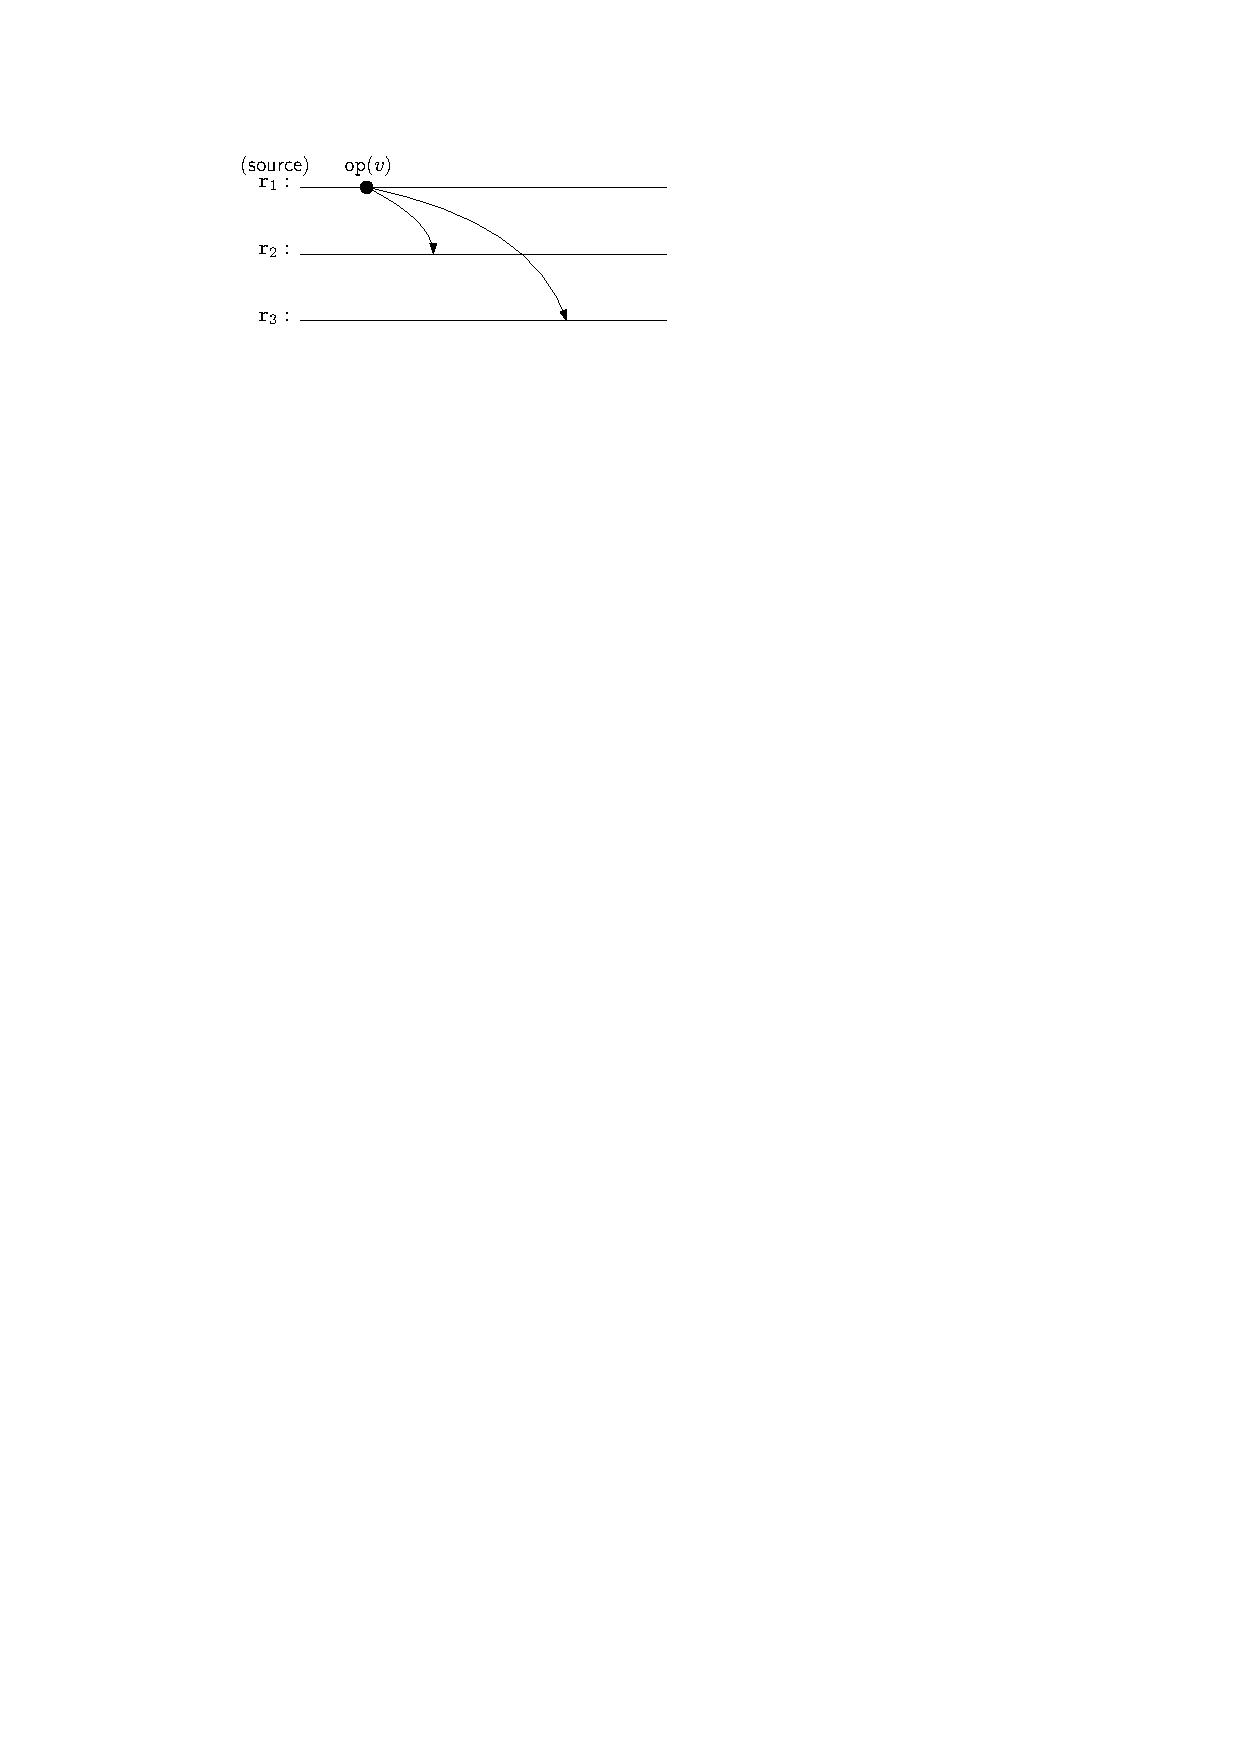
\includegraphics[scale=1]{figures/sys-mod}
  \caption{CRDT System Model}
  \label{fig:sys-mod}
% \end{figure}
\end{wrapfigure}
We assume that the system is comprised of multiple nodes in a network.
In this work we will be concerned with the implementation of CRDTs,
and we will usually concentrate our discussion to the behaviors
allowed for \emph{an instance} of the data type.
We will generically call such an instance an \emph{object}.
As mentioned in~\autoref{sec:introduction} we assume that objects are
replicated among the participating nodes of the system -- which we
shall call replicas.

\gpwarning{Redraw pictures.}
The execution model for an operation \lstinline|op(v)| on a replicated
object is depicted in~\autoref{fig:sys-mod} and it proceeds as follows:
\begin{itemize}
\item A client, which is a program issuing calls to the object, connects
  to any one replica (a node of the system holding a copy of the object)
  and performs the operation in that replica, we shall call such a
  replica the origin or \emph{source}. The source of \lstinline|op(v)|
  in~\autoref{fig:sys-mod} is the replica on the top.
\item Then, executing an operation is done in two phases.
  Assuming that the operation requires reading and updating the state
  of the object, the state of the object in the source replica is read
  first.
  We shall sometimes refer to this part of the operation as the
  generator following~\cite{ShapiroPBZ11}.
  Then, if the state needs to be changed as part of the operation --
  e.g. an \lstinline|addRight| operation of RGA -- an update is
  generated which shall be executed in all the replicas holding copies of the
  object.
  We shall refer to the update as the effector.
  We assume throughout this paper that effectors are executed
  immediate in the source replica.
  This is represented by the dot at the source replica
  in~\autoref{fig:sys-mod}.
\item Finally, as the system progresses, the effector of the operation
  will be delivered to each of the replicas holding a copy of the
  object.
  This is represented by the target of the arrows
  in~\autoref{fig:sys-mod}.
\end{itemize}
% This model is depicted in~\autoref{fig:system-model}.
% \fxwarning[nomargin, inline]{We need the picture}.

\paragraph{CRDT implementations}

Following the description above, \citet{ShapiroPBZ11} presents the code
for a number of CRDT implementations.
%
Here we consider the code of the RGA algorithm presented
in~\autoref{lst:rga}.
%
Let us first consider the structure of the data type implementation:
\begin{itemize}
\item The keyword \lstinline|payload| introduces the state that is
  used to represent the object. This is akin to the fields of a class
  file in an object oriented language such as Java. In the specific
  case of RGA we have a variable \lstinline|N| of type
  \lstinline|Ti-Tree| (to be discussed later), and a variable
  \lstinline|Tomb| of type \lstinline|Set|.
\item After that we find the definitions of the three operations we
  discussed in the introduction: \lstinline|addAfter|,
  \lstinline|remove| and \lstinline|read|.
\item The effectful operations \lstinline|addAfter| and
  \lstinline|remove| have two labels marked in red:
  \lstinline|atSource| and \lstinline|downStream|.
  These represent the code to be executed as the generator and
  effector respectively. Hence, the code under the label
  \lstinline|atSource| is executed only at the source replica and it
  generates the arguments that the code under \lstinline|downStream|
  will execute in each of the replicas.
\item We can also notice that under the labels there are
  \lstinline|precondition| annotations indicating facts that are
  assumed about the state of the object upon execution of either of
  the generator or effector of the operation.
\end{itemize}
Reconsidering~\autoref{fig:sys-mod} we can then say that the
source of the arrows in each replica represent the execution of an
\lstinline|atSource| jointly with the \lstinline|downStream| of the
operation at the source replica.
%
The sink of the arrows represents the delivery and execution of the
generator of the operation in a replica other than the source.


In the rest of this section we consider two examples of CRDT
implementations and their linearization arguments.

\subsection{RGA CRDT Implementation}
\label{sec:rga-crdt-impl}

% \paragraph{RGA CRDT implementation}
As it is common to many CRDT implementations, in RGA replicas will use
a timestamp mechanism to keep track of the causality between updates
to the list, effectively capturing when two updates are concurrent,
and moreover, they will keep the information relating the causal order
in which elements are added to the list.
%
Provided with this causality -- or lack thereof-- information, the
timestamps will be used to resolve conflicts in a deterministic way.
%
More concretely, each replica will keep what we shall name a
\emph{Timestamp Tree} (\lstinline|Ti-Tree|) containing in every tree
node a pair with: the element added to the list (for instance the
character \lstinline|b|), and a timestamp associated to it
(\lstinline|t|$_{\mathtt{b}}$) which will be used to resolve
conflicts.
%
We will encode the tree as a set containing triples (corresponding to
nodes) of the form (\lstinline|a|, \lstinline|ts|$_{\mathtt{b}}$, \lstinline|b|)
representing the fact that there is an element \lstinline|b| in the
tree with timestamp \lstinline|ts|$_{\mathtt{b}}$ and whose parent is the item
\lstinline|a| also present in the tree.
%
The tree-ness property will be ensured by construction.


\begin{wrapfigure}{l}{.3\textwidth}
  \centering
  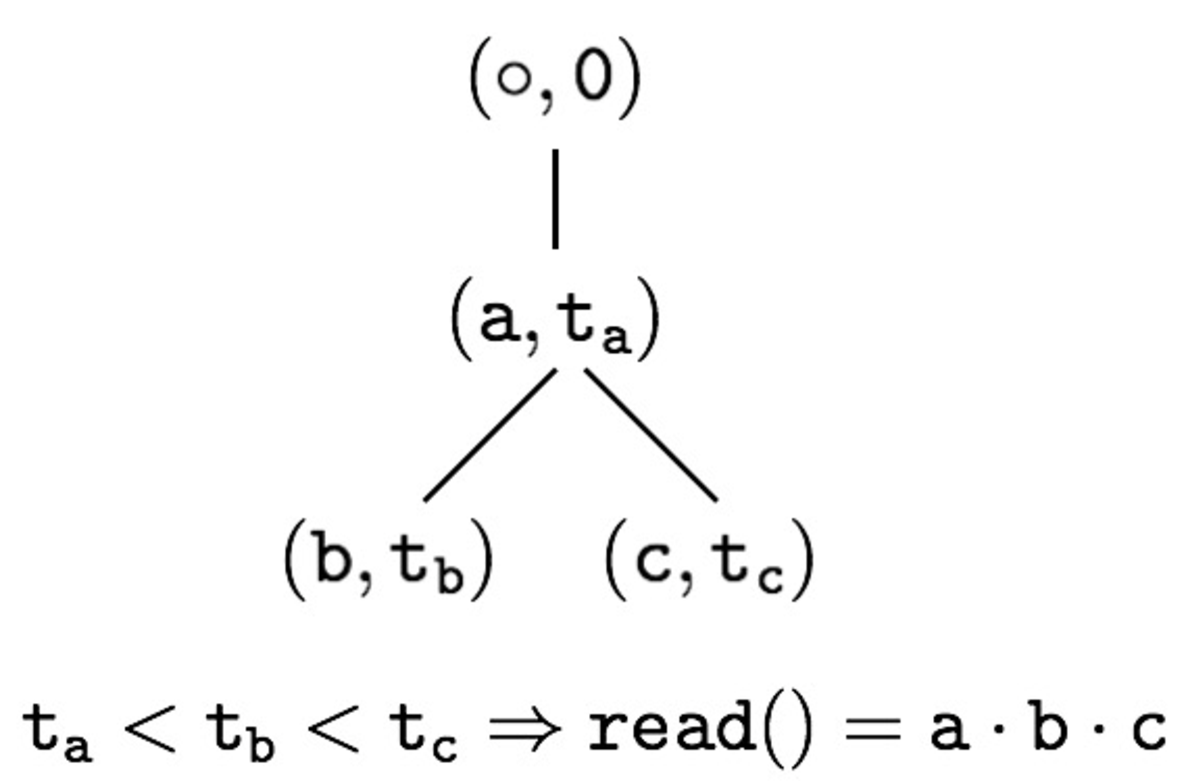
\includegraphics[scale=.9]{figures/simple-ti-tree}
  \caption{RGA Ti-tree example.}
  \label{fig:rga-tree}
\end{wrapfigure} 
If we look at the \lstinline|atSource| portion of the
\lstinline|addAfter(a,b)| method we can see that precondition requires
the \lstinline|a| to exist in the tree before the insertion of
\lstinline|b| after it.
%
We remark at this point that the data structure is initialized with a
preexisting initial element denoted by $\circ$.
%
The generator then samples a timestamp \lstinline|t|$_{\mathtt{b}}$
for \lstinline|b| which is assumed to be larger than any
timestamp presently occurring in the \lstinline|Ti-Tree|
\lstinline|N|.
\gpnote{Add note about uniqueness of TSs (rid).}
%
Looking at the \lstinline|downStream| portion of
\lstinline|addAfter(a,b)| we see that the effect of the operation is
to add the triple \lstinline|(a, ts|$_{\mathtt{b}}$\lstinline|, b)|
in the replicas own copy of \lstinline|N|.
%
Then, the tree structure is consistent with the causality of
insertions in the data structure.
%
Notice that a client of the object will only ever attempt to add an
element after another element which has already seen (mandated by the
\lstinline|addAfter| API).
%
Hence, the parent node of any node was inserted before it, and is
causally related to it.
%
Similarly, nodes that are not related to each other on any path of
the tree (eg. siblings) are not related necessarily causally related.
% \footnote{The converse
%   is not true. There can be nodes that are linked by ancestry in the
%   tree resulting from concurrent operations, but this does not affect
%   the correctness of the algorithm.}
%
An example of such a tree is shown in~\autoref{fig:rga-tree}.

 Considering a \lstinline|Ti-tree| constructed in this way, we can
obtain a list by traversing the tree in pre-order fashion, with the
proviso that siblings are ordered according to their timestamps with
the highest timestamp traversed first.
%
\autoref{fig:rga-tree} shows the tree that results from the given
tree.


\begin{figure}[t]
  \centering
  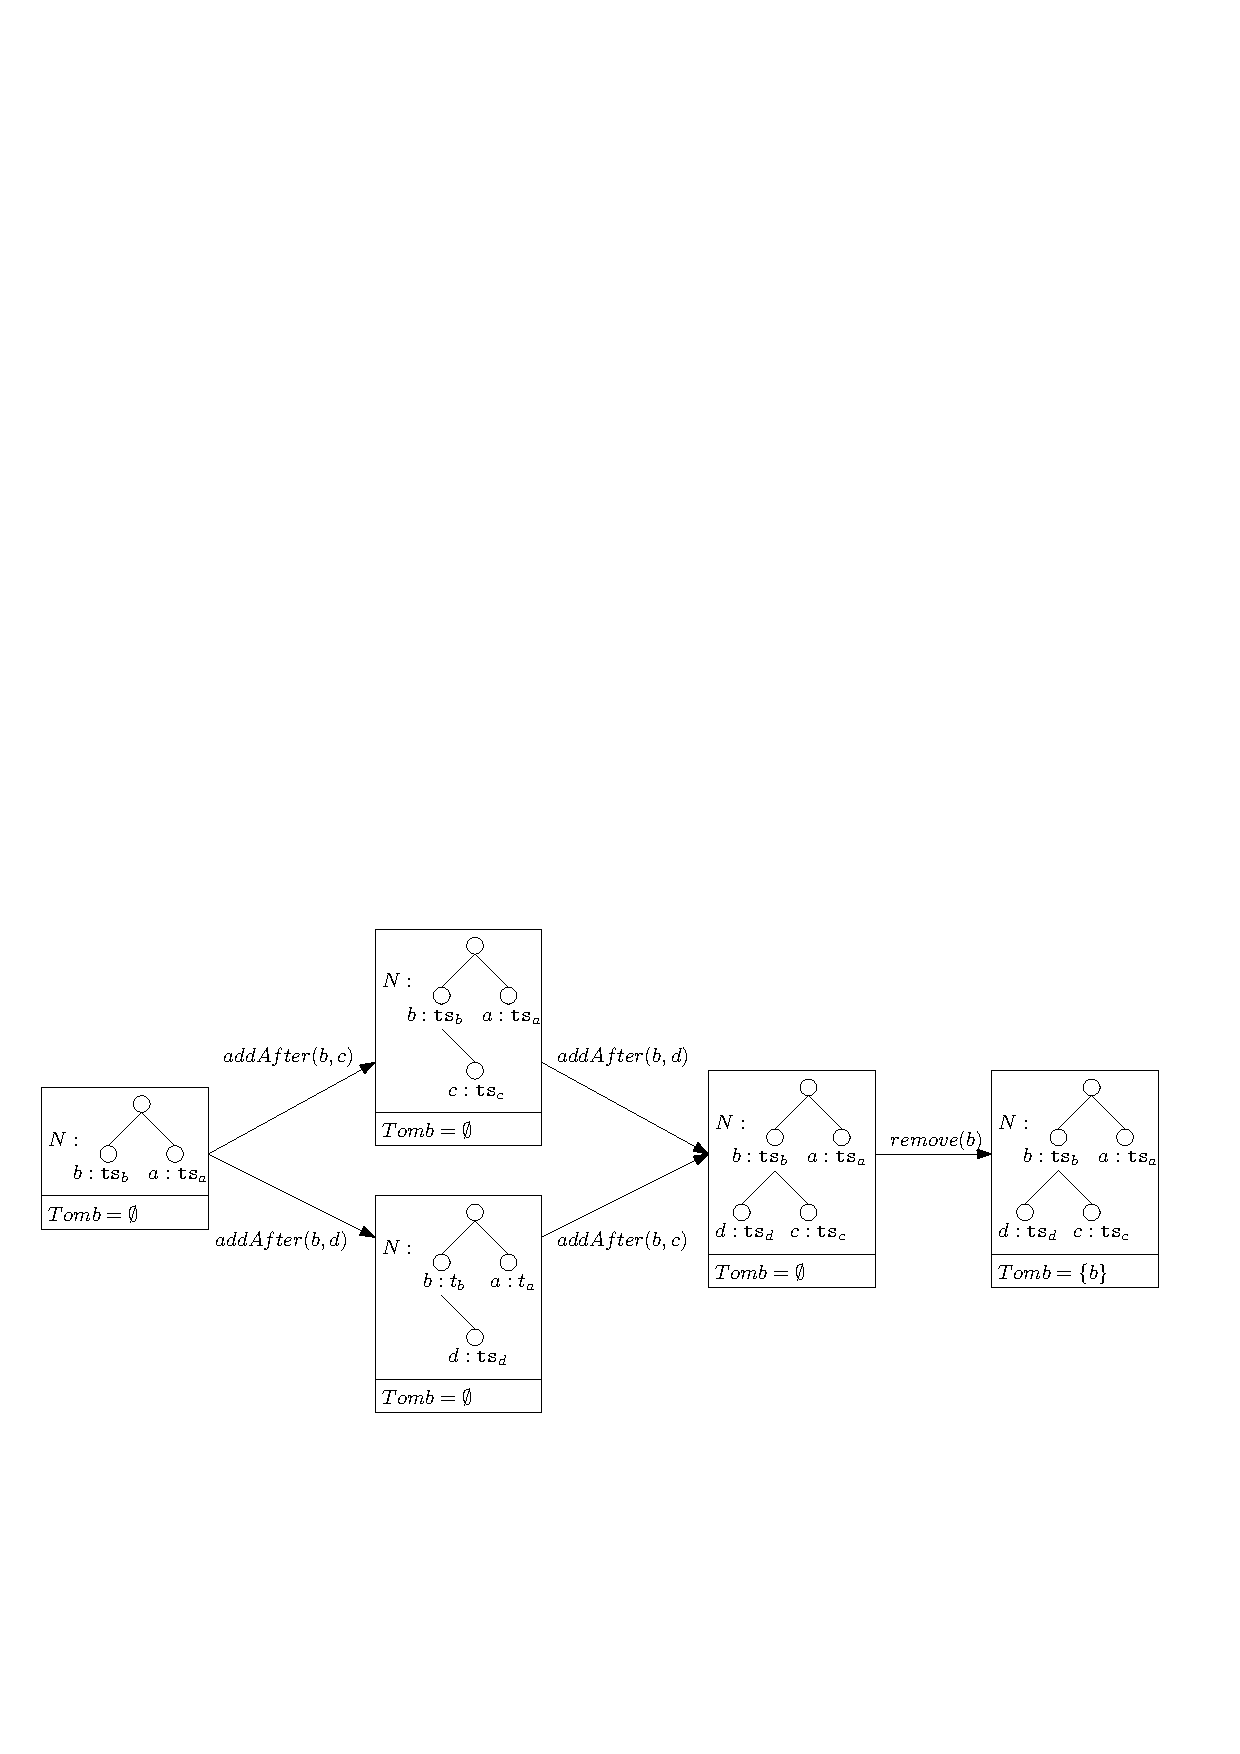
\includegraphics[width=0.85 \textwidth]{figures/HowRGAWork.pdf}
% \vspace{-10pt}
  \caption{An example of conflict resolution of RGA, and how we do remove.}
  \label{fig:how RGA works}
\end{figure}


\gpnote*{By Chao. Should be elsewhere}{
\figurename~\ref{fig:how RGA works} gives a example of how RGA do conflict resolution for concurrent $addAfter$ operations, and how it do $remove$: if from one local state we do concurrent $\alabelshort[addAfter]{b,c}$ and $\alabelshort[addAfter]{b,d}$, then it converges. If we then do $\alabelshort[remove]{b}$, we just add $b$ into tombstone. Here we assume $\ats_a$, $\ats_b$, $\ats_c$ and $\ats_d$ is the timestamp of $a$, $b$, $c$ and $d$, respectively, and the timestamp order be $\ats_a < \ats_b < \ats_c < \ats_d$.
}

We have so far ignored the \lstinline|remove| operation.
%
Consider the case where a client issues an \lstinline|addAfter(a, b)|
on a replica whereas another client issues a \lstinline|remove(a)|
operation in another replica.
%
If the effector of \lstinline|remove(a)| reaches every replica after
the effector of \lstinline|addAfter(a, b)| there is no problem since
the semantics is obvious (the element \lstinline|a| is removed after
the element \lstinline|b| has been added).
%
However, if the operations reach some replica in the opposite order
(recall that these are concurrent operations) we have a problem, since
the precondition of the effector of \lstinline|addAfter(a, b)|
requires that the element \lstinline|a| be present in the
\lstinline|Ti-tree| of the replica.

To avoid this kind of conflict, thus rendering these operations
commutative (c.f. CRDT), RGA does not really erase elements from the
\lstinline|Ti-tree|.
%
Instead, an additional data structure called a tombstone is used to
keep track of elements that have been conceptually erased and should
not be considered when reading the data structure with the
\lstinline|read| operation.
%
In our case the tombstone is simply a set \lstinline|Tomb| of
elements.
%
With this explanation the code of the \lstinline|remove| operation
in~\autoref{lst:rga} should be self-explanatory.

Finally, the implementation of \lstinline|read| performs the pre-order
traversal as explained before, where all the elements in the tombstone
\lstinline|Tomb| are ignored from the output list.

\fxwarning[nomargin, inline]{It's not clear what we are linearizing. I think we should say that standard linearizability considers the partial order given by real-time while here we consider the visibility relation}

\fxwarning[nomargin, inline]{We should already explain the issue of queries, the fact that RGA is not linearizable in the classical sense.}


\paragraph{Intuition of RGA \CRDTLinshort{}}
Let us consider the problem of showing that an execution of an series
of operations on an RGA object is linearizable.
%
That is, that there exists a total order of the operations such that
the result of each operation corresponds to the execution of all the
operations prior to it in the order (c.f.
linearizability~\cite{HerlihyW90}).
%
To simplify the argument which will be made precise in the following
section we focus here on the linearization of two concurrent
operations adding an element after a common element. 
%
Let us say concurrent \lstinline|addAfter(a,b)| and
\lstinline|addAfter(a,c)| operations. 
% 
Can we show that these operations can always be order one way or
another such that the result of all subsequent reads will correspond
to this ordering?
%
In fact, from the explanation given above we know that the order
between \lstinline|b| and \lstinline|c| in the resulting list will be
determined by their corresponding timestamps
(\lstinline|t|$_{\mathtt{b}}$ and \lstinline|t|$_{\mathtt{c}}$). 
%
Assuming that the ordering is the one given in~\autoref{fig:rga-tree}
we know that we can order the operations as \lstinline|addAfter(a, c)|
followed by \lstinline|addAfter(a, b)| which obviously results in
$\mathtt{a \cdot b \cdot c}$ as shown in the picture. 
%
While this is only one case, in~\autoref{sec:proofs} we will show that
all operations can be order in such a way that they correspond to a
sequential execution thereof. 


% In RGA algorithm, a replica store the list as a timestamp insertion
% tree (TI-tree) $N$, and stores the deleted items in tombstone
% $\mathit{Tomb}$. A TI-tree $N$ is a set of tuples $(a,t,p)$, where
% $a$ is a item, $t$ is its unique time-stamp, and $p$ is the
% time-stamp of its ``parent'' node. Each time-stamp is a tuple
% $(c,r)$ with $c \in \mathbb{N}$ and $r \in \mathbb{R}$. A total
% order $<_{\mathit{ts}}$ between time-stamps is defined, such that
% $(c_1,r_1) <_{\mathit{ts}} (c_2,r_2)$, if $c_1 < c_2 \vee (c_1 = c_2
% \wedge r_1 <_r r_2)$, where $<_r$ is a total-order over
% $\mathbb{R}$. There is a pre-existed item $\circ$ of TI-tree with
% time stamp $(0,r_0)$, which are considered as the root of the tree.
% Each element of $N$ should have unique item and time stamp, and the
% elements of $N$ are required to form a tree by following the parent
% field. The tombstone $\mathit{Tomb}$ is a set of items and records
% items been removed from the list.

% \ce{Make the distinction between an operation being
% \emph{originated} at some replica, and whose downstream is
% \emph{executed} at some replica}

% \gpwarning[nomargin, inline]{I think it would be useful to show a
%   graphical example of linearizations here. Something like the
%   examples in the HW paper would do.}

\subsection{OR-Set CRDT Implementation}
\label{sec:or-set-crdt}

\begin{figure}[!t]
  \centering
\begin{lstlisting}[caption={Pseudo-code of the OR-Set CRDT},
captionpos=b,label={lst:or-set}]
  payload Set S
  initial S = @|$\emptyset$|@
  //@ initial lin = @|$\epsilon$|@

  add(a) :
    atSource :
      let k = getUniqueIdentifier()
      //@ let lin@|$'$|@ = lin@|$\,\cdot\,$|@add(a,k)
    downStream(a, k) :
      S = S @|$\cup$|@ {(a, k)}
      //@ S@|$'$|@ = S @|$\cup$|@ {(a, k)}

  remove(a) :
    atSource :
      let R = {(a,k) | (a,k) @|$\in$|@ S}
      //@ let lin = lin@|$\,\cdot\,$|@readIds(a)@|$\Rightarrow$|@R@|$\,\cdot\,$|@remove(a,R)
    downStream(R) :
      S = S @|$\setminus$|@ R
      //@ R == {(a,k) | @|$\exists\ \alabel$|@ = add(a,k)@|$\Rightarrow$|@, (@|$\alabel$|@, remove(a,R))@|$\in \avisord\ \land$|@
                             @|$ \forall\ \alabel'$|@ = remove(a,*)@|$\Rightarrow$|@, {(@|$\alabel,\alabel'$|@),(@|$\alabel'$|@, remove(a,R))}@|$\not\subseteq\,\avisord$|@}
      //@ S@|$'$|@ = S @|$\setminus$|@ R@|$'$|@

  read() :
    let A = {a : @|$\exists$|@ k. (a,k) @|$\in$|@ S}
    //@ let lin@|$'$|@ = lin@|$\,\cdot\,$|@read@|$\Rightarrow$|@A
    return A
\end{lstlisting}
\end{figure}
      % //@ R' = @|$\{ (a,k): \exists\ \alabel = \alabellongind[{\tt add}]{a,k}{\bot}{*}.\ (\alabel, \alabelshort[{\tt remove}]{a,R}) \in \avisord$|@
      %                  @|$\land\,\forall\ \alabel' = \alabellongind[{\tt remove}]{a,*}{\bot}{*}.\ \{(\alabel,\alabel'),(\alabel',\alabelshort[{\tt remove}]{a,R})\}\not\subseteq \avisord\}$|@
      % //@ S@|$'$|@ = S @|$\setminus$|@ R

The Observed-Remove Set (OR-Set) is another CRDT~\cite{ShapiroPBZ11},
this time implementing a Set interface with methods: \lstinline|add(a)|,
\lstinline|remove(a)| and \lstinline|read()|.\footnote{Alternatively
  we could provide an interface with the method \lstinline|lookup(a)|
  returning a boolean with the same consequences as the
  \lstinline|read()| method we provide.}
%
The meaning of these methods is self-evident from their names.
%
However, what is not evident is what are the results of conflicting
concurrent operations.
%
Consider for example the case where two replicas add a certain element
\lstinline|a| and then one of them removes that element.
%
% \gpnote[nomargin, inline]{Add picture.}
If we consider an interleaving based execution of these operations
there are two options depending on the interleaving:
\begin{inparaenum}[i)]
\item if the \lstinline|remove(a)| operation is the last operation
  then the expected set is empty, since the two consecutive
  \lstinline|add(a)| operations are idempotent, and the
  \lstinline|remove| would remove the only occurrence of
  \lstinline|a|. This interleaving is the one depicted with solid
  arrows at the top of~\autoref{fig:or-set-not-lin}.
\item On the other hand, if the operation \lstinline|add(a)| of the
  non-removing process comes last, the final set could contain the
  element \lstinline|a| as depicted with the dashed arrows
  in~\autoref{fig:or-set-not-lin}.
\end{inparaenum}
As we have explained before, in our system model the operations can
arrive in one order to one replica and in a different order to another
replica.
%
To guarantee convergence, OR-Set must ensure that regardless of the
ordering, the resulting set will be the same.
%
To that end, OR-Set \lstinline|add| operations will tag each added
element with a unique identifier.
%
Then, a remove operation will only remove the elements which has
already seen.
%
For instance, in the example above, the remove of \lstinline|a| will
only remove the element that has been previously added by in the same
replica, since this item as been observed by the \lstinline|remove|
operation -- and thus its identifier is known to it --. However, the
concurrent \lstinline|add(a)| operation will have an identifier that
has not been observed by the \lstinline|remove| (since they are
concurrent).
%
Therefore the item will not be removed, even in the case where the
effectors of the two adds are performed in a replica before the effector
of the remove.
%
The code of OR-Set is shown in~\autoref{lst:or-set} where for the time
being we ignore the lines marked with a comment (\lstinline|//@|).

\fxwarning[nomargin, inline]{If queries are discussed already for RGA, here we should focus more on the rewriting of labels}

\paragraph{Intuition of OR-Set Linearizability}
\gpnote{Add reads at the end of the pictures.}


It is easy to find examples where the implementation of OR-Set can
produce executions which cannot be justified by standard definition of
linearizability (they are not even sequentializable)
of~\citet{HerlihyW90} assuming a standard set specification.
%
\gpwarning{Redraw this picture properly.}
\autoref{fig:or-set-not-lin} shows one such example.
%
For simplicity we assume here that we have two clients, each executing
in one of two replicas as their source, issuing the sequences of
operations \lstinline|add(b);add(a);remove(b)| and
\lstinline|add(a);add(b);remove(a)| respectively.
%
Clearly any linearization a la~\citet{HerlihyW90} should end with a
\lstinline|remove| operation, and therefore the final set should have
at most one element, contrary to that, in the final set we obtain:
\{\lstinline|a, b|\}.
%
In other words, if in any of the replicas a \lstinline|read()|
operation were to be issued, the result would be the set
\{\lstinline|a, b|\} .

\begin{figure}[t]
  \centering
  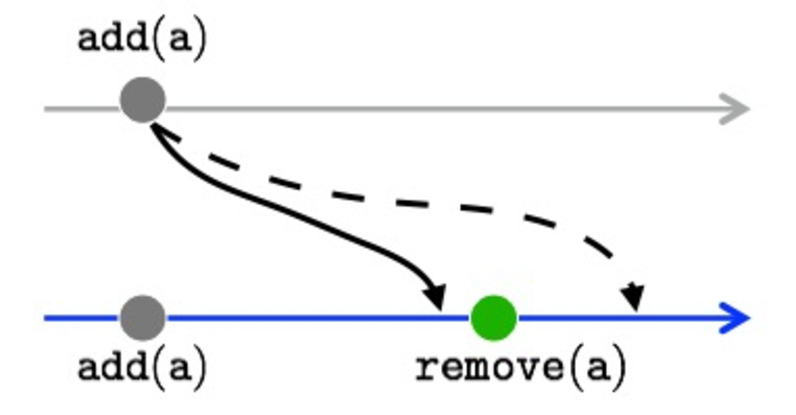
\includegraphics[width=0.40 \textwidth]{./figures/OR-Set-simple}
  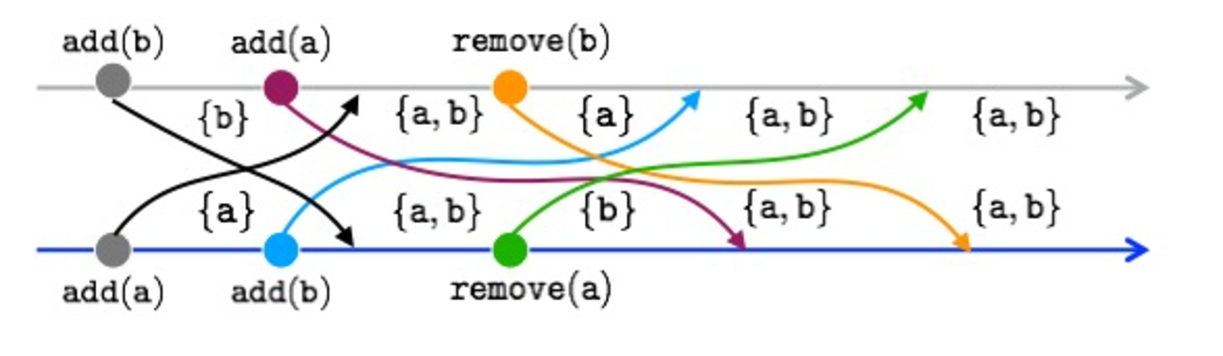
\includegraphics[width=0.70 \textwidth]{./figures/OR-Set-weird}
  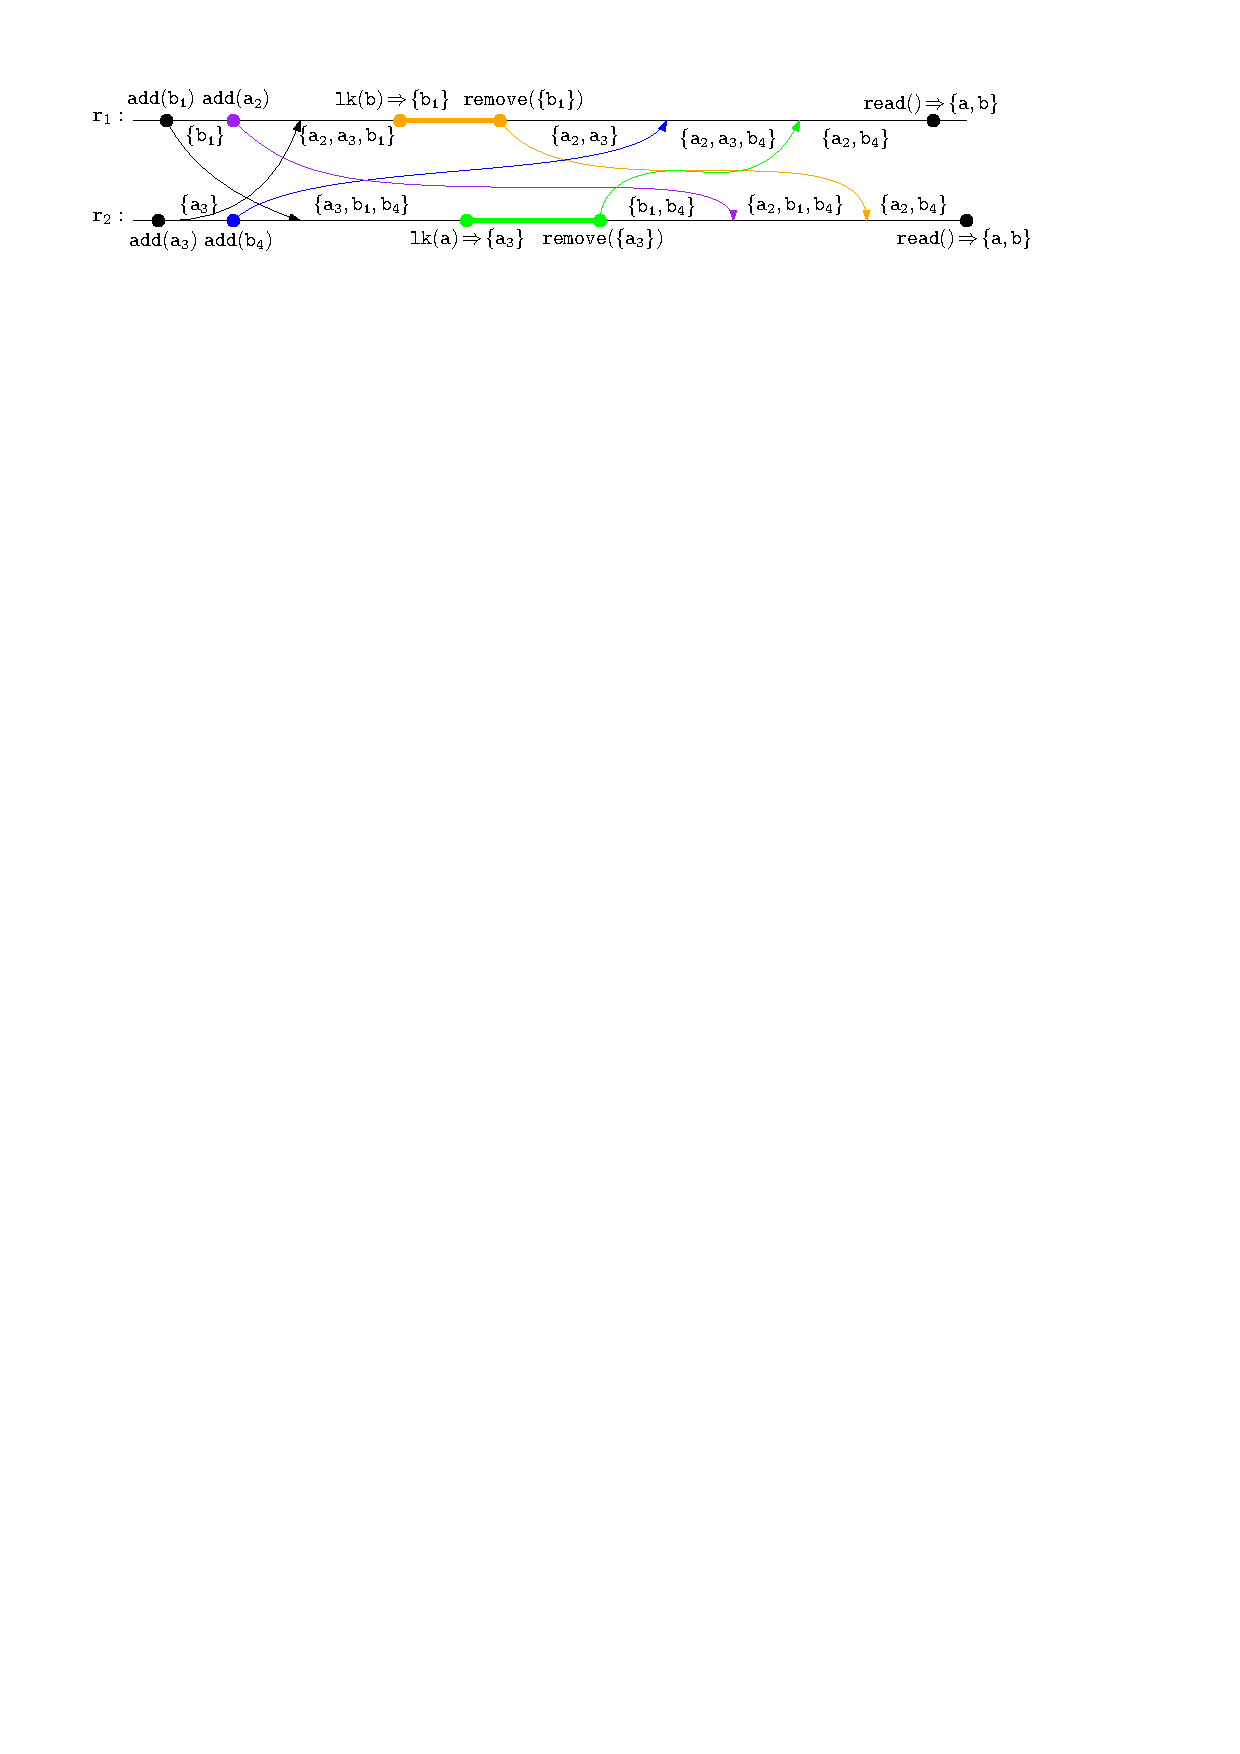
\includegraphics[width=0.90 \textwidth]{./figures/OR-Set-lk-rem}
  \caption{OR-Set non-linearizable execution.}
  \label{fig:or-set-not-lin}
\end{figure}

For our definition of \CRDTLinshort{} we will distinguish between
\emph{update} and \emph{query} operations.
%
We will impose two constraints, one on updates and the other on
queries:
\begin{itemize}
\item For updates we require that there exists a total order of all
  the updates in the execution -- essentially a linearization -- such
  that the resulting state of the object -- or any intermediate state --
  can be explained by executing the \emph{specification} of these
  updates in order.
%
  Essentially, reachable states of the implementation are related to
  specification states that can be reached by a certain linearization of
  the updates.
%
  \gpnote{Example?}
\item Unfortunately, this simple requirement does not suffice for
  query operations, since the system model allows for updates to arrive
  to different replicas in different order.
%
  Hence, for \CRDTLinshort{} we will require that the result of any
  query can be explained by consider a \emph{sub-sequence} of the above
  mentioned global linearization up updates.
\end{itemize}
This definition will be made precise in~\autoref{sec:distributed-lin}.

\gpnote{Maybe add a read example first?}
Coming back to our OR-Set example in~\autoref{fig:or-set-not-lin}, we
have that the \lstinline|remove| operation behaves as both a query
(observing a certain number of updates on the element to be removed)
and an update (by removing said updates).
%
To cope with such cases, we will consider in our definition that
query-update operations can be split into a query part, which only
reads the state -- and hence can see only a sub-sequence of the
linearization of updates --, and an update part which will use the
results of the prior query.
%
For instance, \lstinline|remove| will be split into a query part where
only the elements that are visible at the time of the remove are
selected, and an update part where only those elements selected are
erased.
%
Evidently, this requires some mechanism for ``marking'' the adds that
are concerned.
%
We will consider that each add has a unique identifier.
%
Then, the query part of a remove returns a set of unique identifiers
to be removed.
%
Any identifier not in this set will remain in the set after the update
part of the remove.
%
The second part of~\autoref{fig:or-set-not-lin} shows this rewriting
where we denote by \lstinline|lk| (for lookup) the query part of
remove, which returns a set of elements to be removed, and a
\lstinline|remove| operation taking a set of elements to be removed.
%
In this case, our definition of linearizability is just as before.
%
To linearize this execution, when contemplating only the updates, we
can chose any order consistent with the order in which operations are
performed in each replica and the result is consistent with the
specification of a set.
%
We discuss the details of this constructions in the next section.


% Method $\mathit{add}(a,b)$ intends to add item $a$ into the list at a
% position immediately after that of a existing item $b$. Method
% $\mathit{rem}(a)$ removes $a$ from the list. Method $\mathit{read}$
% returns the current list content. When the current replica does
% $\mathit{add}(a,b)$, it generate a tuple $(a,ts_a,ts_b)$ and put it
% into $N$. Here $ts_b$ is the time-stamp of $b$, and $ts_a$ is a new
% time-stamp that is larger than any time stamp in $N$. When the current
% replica does $\mathit{rem}(a)$, it put $a$ into tombstone. When the
% current replica does $\mathit{read}$, it uses function
% $\mathit{trans}(N,\mathit{Tomb})$ to return the list seen by the
% current replica, which is a sequences obtained by traversing $N$ in
% prefix order (children are visited in decreasing time-stamp order) and
% keeping only items that are not in $\mathit{Tomb}$.

%      precondition : %@|$\exists$|@ k. (a,k) @|$\in$|@ S
%let @|$\alabel = \alabellongind[remove]{a,R}{\bot}{i}$|@
%      //@ @|$\alpha(S) \xrightarrow{\alabelshort[add]{a,k}} \alpha(S')$|@
%       //@ @|$\alpha(S) \xrightarrow{\alabellongind[readIds]{a}{R}{}} \alpha(S)$|@
%       //@ @|$\alpha(S) \xrightarrow{\alabelshort[remove]{a,R}} \alpha(S')$|@
%     //@ @|$\alpha(S) \xrightarrow{\alabellongind[read]{}{A}{}} \alpha(S)$|@

% In the downstream of a $\alabellongNoret[\mathit{add}]{\argv}$
% operation, an tuple $(\argv,\ats)$ will be added to the local state;
% while in the downstream of a $\alabellongNoret[\mathit{add}]{\argv}$
% operation, a set $S_1$ will be removed from the local state. We call
% such tuple $(\argv,\ats)$ or set $S_1$ the content of the downstream.
% The following is the condition $C_2$ for or-set implementati.

%%% Local Variables:
%%% mode: latex
%%% TeX-master: "draft"
%%% End:


%%!TEX root = draft.tex

\section{CRDT Implementations}
\label{sec:CRDT implementations}



%Let $\mathbb{MSG}$ be the set of message contents, such as $(a,ts_a,ts_b)$ of RGA. Then, CRDT implementations are defined as follows, where operations and receiving messages are defined as functions.
%
%\begin{definition}[CRDT implementations]
%\label{definition:operation-based CRDT implementations}
%A CRDT implementation for a type $t = (M,D)$ is a tuple $I(r) = (\Sigma, \Sigma_0, \mathit{Msg}, \mathit{do},\mathit{receive})$. Here $r \in \mathbb{R}$, $\Sigma_0 \subseteq \Sigma$, $\mathit{Msg} \subseteq \mathbb{MSG}$, $\mathit{do}:\Sigma \times M \times D \rightarrow \Sigma \times D \times (\mathit{Msg} \cup \{ \emptyset \} )$, and $\mathit{receive}: \Sigma \times \mathit{Msg} \rightarrow \Sigma$.
%\end{definition}
%
%Here $\Sigma$ is the set of local states and $\Sigma_0$ is the set of initial state. $r$ is the replica identifier of current replica, and some CRDT implementation requires current replica identifier to generate time-stamp. When the current local state is $\sigma$ and the client intends to perform a operation of method $m$ with argument $a$, a $\mathit{do}$ action is launched, which update the local states, returns a value, and generate message if $m$ is a update method. When this replica receives a message of other replica, a $\mathit{receive}$ action will be launched, which updates the current local states according to the message. If a operation has no arguments or return value, or does not generate message, then we can safely omit the corresponding tuples in $\mathit{do}$ action.
%% The formal definition of RGA can be easily obtained from its algorithms. For example, when $(a,\_,\_) \in N$, we have $\mathit{do}((N,\mathit{Tomb}),\mathit{rem},a) = ((N,\mathit{Tomb} \cup \{ a \}),a)$. Here we use $\_$ in indicate a element whose value is irrelevant.
%The formal definition of RGA, as well as more CRDT implementations, can be found in  Appendix \ref{sec:appendix definitions of section CRDT implementations}.

















\forget{
\section{CRDT Implementations}
\label{sec:CRDT implementations}

A distributed system contains multiple objects, and each objects is replicated on each replica. Each object has a type, which contains its method and data type. A client of a replica interact with the objects by calling the method and then obtaining the return value. Here we do not bound the number of replica identifiers and objects.

Let $\mathbb{OBJ}$ be the set of objects and $\mathbb{R}$ be the set of replica identifiers. We consider a finite set $\mathbb{M}$ of method names; and a possibly infinite set $\mathbb{D}$ of arguments and return values, the data domain. Each data type $t = (M,D)$ has a set $M \subseteq \mathbb{M}$ of methods and a data domain $D \subseteq \mathbb{D}$. Finally we have a infinite set $\mathbb{OID}$ of operation identifiers, corresponding to each individual operation performed on the CRDT throughout an execution.

Without loss of generality we will consider that the methods in $\mathbb{M}$ can be separated in two disjoint sets of methods: $\mathbb{Q}$ query methods that has no influence on the ``abstract state'' and normally returns an observation of the ``abstract state'' , and $\mathbb{U}$ update methods that has influence on the ``abstract state''. Note that some update operation also need to read the ``abstract state''. For example, a $add(a,b)$ operation is an operation of distributed list which intends to put item $a$ immediately after item $b$. This operation implicitly requires that item $b$ is already in list.

$\mathit{Optimistic \ replication \ algorithms}$ is a type of distributed algorithms where each client contains a copy of data structure; a client operations takes effect instantly at its replica without any synchronization, and then broadcast to other replicas and got applied. Convergent or Commutative Replicated Data Types (CRDTs) is a typical kinds of optimistic replication algorithms. In this section, we will introduce CRDT algorithms and their formation.

In practice, there are two kinds of CRDT implementations: state-based CRDT and operation-based CRDT. In state-based CRDT, a update operation take effects locally; in nondeterministic time, a replica may decide to send the (modified) local state into other replicas. The state-based PN-counter is an example of state-based CRDT algorithms and is shown below. Keyword $\mathit{payload}$ indicate the local state, and keyword $\mathit{initial}$ specifies the initial value of local state. Function $\mathit{myID}()$ returns the current replica identifier, and $\mathit{reps}()$ returns the number of replicas of the distributed system. Vector $P$ (resp., $N$) is a vector such that $P[i]$ (resp., $N[i]$) is the number of increase that is generated by replica $i$ and is observed by current replica. This algorithm assumes that the set of replica is already known and is fixed and finite.

Method $\mathit{inc}$ increase the counter by $1$, method $\mathit{dec}$ decrease the counter by $1$, and method $\mathit{read}$ returns the current counter value. Assume the replica identifier of current replica is $r$. When the current replica does $\mathit{inc}$, it modify $P[r]$ into $P[r]+1$. When the current replica does $\mathit{dec}$, it modify $N[r]$ into $N[r]+1$. When the current replica does $\mathit{read}$, it returns $\Sigma_{i}^{n} P[i] - \Sigma_{i}^{n} N[i]$. When the current replica receive a message of modified payload $Z$, it uses function $\mathit{merge}()$ to update the current local state. $\mathit{merge}$ takes the maximum of each replica in the vector.

\renewcommand{\algorithmcfname}{CRDT Implementation}
\noindent
%\begin{minipage}{.5\textwidth}
\noindent\begin{algorithm}[H]
$\mathit{payload}$ integer[$\mathit{reps}$()] P, integer[$\mathit{reps}$()] N; \\
$\mathit{initial}$ [0,\ldots,0],[0,\ldots,0]; \\

$\mathit{inc}()$ \\
%\ \ \ \ let \ g = myID();\\
\ \ \ \ P[$\mathit{myID}$()] = P[$\mathit{myID}$()] + 1; \\

$\mathit{dec}()$ \\
%\ \ \ \ let \ g = myID();\\
\ \ \ \ N[$\mathit{myID}$()] = N[$\mathit{myID}$()] + 1; \\

$\mathit{read}()$ \\
\ \ \ \ \KwRet $\Sigma_{i}^{n} P[i] - \Sigma_{i}^{n} N[i]$; \\

$\mathit{merge}(Z)$ \\
\ \ \ \ $\forall i$, $P[i] = \mathit{max}(P[i],Z.P[i])$; \\
\ \ \ \ $\forall i$, $N[i] = \mathit{max}(N[i],Z.N[i])$; \\
\caption{State-based PN-counter}
\label{Method1}
\end{algorithm}

In operation-based CRDT, an update operation not only updates its local state, but also sends a description of this operation into other replica. Here we take a more complex algorithm, replicated growable array (RGA), as an example of operation-based CRDT and it is shown below.

\renewcommand{\algorithmcfname}{CRDT Implementation}
\noindent
%\begin{minipage}{.5\textwidth}
\noindent\begin{algorithm}[H]
$\mathit{payload}$ TI-tree N, set $\mathit{Tomb}$; \\
$\mathit{initial}$ $\emptyset$,$\emptyset$; \\

$add(a,b)$ \\
\ \ $\mathit{atSource}$: \\
\ \ \ \ $\mathit{pre}$: \ $b = \circ \vee ( b \neq \circ \wedge (b,\_,\_) \in N \wedge b \notin \mathit{Tomb})$ \\

%\ \ \ \ \If {$N = \emptyset$}
%    { \ \ \ \ let \ $ts_a$ = (myID(),1); \\ }
%\ \ \ \ \Else
%    {\ \ \ \ let \ $ts_a$ = (myID(),$\mathit{max}\{ c' \vert (\_,(\_,c'),\_) \in N \} +1$); \\ }

%\ \ \ \ \If {$b = \circ$}
%    { \ \ \ \ let \ $ts_b$ = (0,0); \\ }
%\ \ \ \ \Else
%    { \ \ \ \ let \ $ts_b$ be time-stamp of $b$ in $N$; \\ }

\ \ \ \ let \ $ts_a$ = ($N = \emptyset$) ? (1,$\mathit{myID}$()) ! ($\mathit{max}\{ c' \vert (\_,(\_,c'),\_) \in N \} +1$,$\mathit{myID}$()); \\
\ \ \ \ let \ $ts_b$ = ($b = \circ$) ? (0,$r_0$) ! (the time-stamp of $b$ in $N$); \\

\ \ $\mathit{downstream}(a,ts_a,ts_b)$: \\
\ \ \ \ $\mathit{pre}$: \ $b = \circ \vee ( b \neq \circ \wedge (b,ts_b,\_) \in N)$ \\

\ \ \ \ $N = N \cup \{ (a,ts_a,ts_b) \}$.


$rem(a)$ \\
\ \ $\mathit{atSource}$: \\
\ \ \ \ $\mathit{pre}$: \ $a \neq \circ \wedge (a,\_,\_) \in N \wedge a \notin \mathit{Tomb}$ \\

\ \ $\mathit{downstream}(a)$: $\mathit{pre}$ \ $a \neq \circ \wedge (a,\_,\_) \in N)$

\ \ \ \ $\mathit{Tomb} = \mathit{Tomb} \cup \{ a \}$.

$read()$ \\
\ \ \ \ \KwRet $\mathit{trans}(N,\mathit{Tomb})$; \\

\caption{RGA}
\label{Method1}
\end{algorithm}

Each update operation of operation-based CRDT ie executed with two phases: Its first phase, marked $\mathit{atSource}$, is local to the current replica. It is enabled if its (optional) pre-condition, marked $\mathit{pre}$, is true currently in local state. It generates the information to be delivered, which is the argument of $\mathit{downstream}$. Note that this phase does not modify the local state. Its second phase, marked $\mathit{downstream}$, executed immediate after the current replica, and asynchronously at other replica when they receive the message of this operation. It is enabled if its (optional) pre-condition is true.

In RGA algorithm, a replica store the list as a timestamp insertion tree (TI-tree) $N$, and stores the deleted items in tombstone $\mathit{Tomb}$. A TI-tree $N$ is a set of tuples $(a,t,p)$, where $a$ is a item, $t$ is its unique time-stamp, and $p$ is the time-stamp of its ``parent'' node. Each time-stamp is a tuple $(c,r)$ with $c \in \mathbb{N}$ and $r \in \mathbb{R}$. A order $<_{\mathit{ts}}$ between time-stamps is defined, such that $(c_1,r_1) <_{\mathit{ts}} (c_2,r_2)$, if $c_1 < c_2 \vee (c_1 = c_2 \wedge r_1 <_r r_2)$, where $<_r$ is a total-order over $\mathbb{R}$. There is a pre-existed item $\circ$ of TI-tree with time stamp $(0,r_0)$, which are considered as the root of the tree. Each element of $N$ should have unique item and time stamp, and the elements of $N$ are required to form a tree by following the parent field. The tombstone $\mathit{Tomb}$ is a set of items and records items been removed from the list.

Method $\mathit{add}(a,b)$ intends to add item $a$ into the list immediately after a existing item $b$. Method $\mathit{rem}(a)$ removes $a$ from the list. Method $\mathit{read}$ returns the current list content. When the current replica does $\mathit{add}(a,b)$, it generate a tuple $(a,ts_a,ts_b)$ and put it into $N$. Here $ts_b$ is the time-stamp of $b$, and $ts_a$ is a new time-stamp that is larger than any time stamp in $N$. When the current replica does $\mathit{rem}(a)$, it put $a$ into tombstone. When the current replica does $\mathit{read}$, it uses function $\mathit{trans}(N,\mathit{Tomb})$ to return the list seen by the current replica, which is a sequences obtained by traversing $N$ in prefix order (children are visited in decreasing time-stamp order) and keeping only items that are not in $\mathit{Tomb}$.


Multi-value register is also a common-used data structures and its sequential specification is nondeterministic and thus different from that of the previous two examples, which are deterministic (seen in the next section). A state-based multi-value register algorithm is shown below.


\renewcommand{\algorithmcfname}{CRDT Implementation}
\noindent
%\begin{minipage}{.5\textwidth}
\noindent\begin{algorithm}[H]
$\mathit{payload}$ $S \subseteq D \times \mathbb{N}^{\mathit{reps}()}$; \\
$\mathit{initial}$ $\emptyset$; \\

$\mathit{write}(a)$ \\
\ \ \ \ let \ g = $\mathit{myID}$(); \\
\ \ \ \ let $\mathcal{V} = \{ V \vert \exists x, (x,V) \in S \}$; \\
\ \ \ \ let $V' = [ \mathit{max}_{V \in \mathcal{V}} V[j] ]_{j \neq g}$; \\
\ \ \ \ let $V'[g] = (\mathit{max}_{V \in \mathcal{V}} V[g]) + 1$; \\
\ \ \ \ $S = (a,V')$; \\

$\mathit{read}()$ \\
\ \ \ \ \KwRet $S' = \{ a \vert (a,\_) \in S \}$; \\

$\mathit{merge}(Z)$ \\
\ \ \ \ let $A' = \{ (x,V) \in S \vert \forall (x',V') \in Z.S, \exists i, V[i] \geq V'[i] \}$; \\
\ \ \ \ let $B' = \{ (x,V) \in Z.S \vert \forall (x',V') \in S, \exists i, V[i] \geq V'[i] \}$; \\
\ \ \ \ $S = A' \cup B'$; \\
\caption{state-based multi-value register}
\label{Method1}
\end{algorithm}

Each replica stores a set $S$ of items such that each item can not dominate other items. To do conflict resolution, we associate each item $a$ in $S$ with a version vector $V$. We say version vector $V$ dominates version vector $V'$, if $\forall i$, $V[i] > V'[i]$.

Method $\mathit{write}(a)$ intends to write $a$ into register. Method $\mathit{read}$ returns the current register content. When the current replica does $\mathit{write}(a)$, it generates a new version vector that dominates all previous ones in $S$. When the current replica does $\mathit{read}$, it returns the set of items in $S$. When the current replica receive a message of modified payload $Z$, we takes the union of every items in $S$ and $Z.S$ whose version vector is not dominated by that of an item in the other set. This algorithm assumes that the set of replica is already known and is fixed and finite.


To enable formally verification of CRDT algorithms, it is necessary to give formal definition of CRDT-algorithms. Let $\mathbb{MSG}$ be the set of message contents, such as $(P,N)$ of state-based PN-counter, or $(a,ts_a,ts_b)$ of RGA. Then, CRDT implementations are defined as follows, where operations and receiving messages are defined as functions.

\begin{definition}[operation-based CRDT implementations]
\label{definition:operation-based CRDT implementations}
A operation-based CRDT implementation for a type $t = (M,D)$ is a tuple $I_t(r) = (\Sigma, \Sigma_0, \mathit{Msg}, \mathit{do},\mathit{receive})$. Here $r \in \mathbb{R}$, $\Sigma_0 \subseteq \Sigma$, $\mathit{Msg} \subseteq \mathbb{MSG}$, $\mathit{do}:\Sigma \times M \times D \rightarrow \Sigma \times D \times (\mathit{Msg} \cup \{ \emptyset \} )$, and $\mathit{receive}: \Sigma \times \mathit{Msg} \rightarrow \Sigma$.
\end{definition}

Here $\Sigma$ is the set of local states and $\Sigma_0$ is the set of initial state. For example, in state-based PN-counter, since there are many possibility of total number of replicas, $\Sigma_0$ is a set of more than one elements. $r$ is the replica identifier of current replica. The reason of containing $r$ in the definition of CRDT implementations is that, some algorithms need the current replica identifier to generate time-stamp. When the current local state is $\sigma$ and the client intends to perform a operation of method $m$ with argument $a$, a $\mathit{do}$ action is launched, which update the local states, returns a value, and possibly generate messages. A $\mathit{do}$ action of update method will generate messages, while a $\mathit{do}$ action of query method will not generate message. When this replica receives a message of other replica, a $\mathit{receive}$ action will be launched, which updates the current local states according to the message. If a operation has no arguments or return value, or does not generate message, then we can safely omit the corresponding tuples in $\mathit{do}$ actions.

\begin{definition}[state-based CRDT implementations]
\label{definition:state-based CRDT implementations}
A state-based CRDT implementation for a type $t = (M,D)$ is a tuple $I_t(r) = (\Sigma, \Sigma_0, \mathit{Msg}, \mathit{do},\mathit{receive})$. Here $r \in \mathbb{R}$, $\Sigma_0 \subseteq \Sigma$, $\mathit{Msg} \subseteq \Sigma$, $\mathit{do}:\Sigma \times M \times D \rightarrow \Sigma \times D$, and $\mathit{receive}: \Sigma \times \Sigma \rightarrow \Sigma$.
\end{definition}

The state-based CRDT implementation is similarly defined. The difference is that, each operation does not send message, and the message content is fixed to be a local state. The following is an example of formal definition of state-based PN-counter. The formal definition of more CRDT implementations are given in Appendix \ref{sec:appendix definitions of section CRDT implementations}. Here we denote by $f[i:j]$ the function that has the same value as $f$ everywhere, except for $i$, where it has the value $j$. %Since each operation is executed without synchronization, it is not hard to obtain formal definition from informal algorithms.

\begin{example}[formal definition of state-based PN-counter]
\label{definition:formal definition of state-based PN-counter}
$I_t(r) = (\Sigma, \sigma_0, \mathit{Msg}, \mathit{do},\mathit{receive})$, where

\begin{itemize}
\setlength{\itemsep}{0.5pt}
\item[-] $\Sigma = \{ (P,N) \vert$, $P$ and $N$ are vector of integers with same length $\}$. $\Sigma_0 = \{ (P_0,N_0) \vert (P_0,N_0) \in \Sigma$, $P_0$ and $N_0$ maps each index into $0 \}$.

\item[-] $\mathit{Msg} \subseteq \Sigma$.

\item[-] $\mathit{do}((P,N),\mathit{inc}) = (P[r:P[r]+1],N)$,

\item[-] $\mathit{do}((P,N),\mathit{dec}) = (P,N[r:N[r]+1])$,

\item[-] $\mathit{receive}((P,N),(P',N')) = (\lambda s. \mathit{max}\{  P[s], N'[s] \}, \mathit{max}\{  N[s], N'[s] \},)$,
\end{itemize}
\end{example}
}































%%% Local Variables:
%%% mode: latex
%%% TeX-master: "draft"
%%% End:

%
%%!TEX root = draft.tex
%\newcommand{\seqPQ}{\mathsf{SeqPQ}}


\section{Definition of Linearizability}
\label{sec:definition of linearizability} 

Let us start our formation of executions, specifications and linearizations of CRDT.  

We consider a finite set $\mathbb{M}$ of method names; and a possibly infinite set $\mathbb{D}$ of arguments and return values, the data domain. Without loss of generality we will consider that the methods in $\mathbb{M}$ can be separated in two disjoint sets of $\mathbb{Q}$ query methods, and $\mathbb{U}$ update methods. We consider replicated data types which are distributed across a set of replicas; the set of replica identifiers is denoted by $\mathbb{R}$. We assume that each replica contains a copy of the data type state. Finally we have a infinite set $\mathbb{O}$ of operation identifiers, corresponding to each individual operation performed on the CRDT throughout an execution.

Operation labels \mbox{$m(a)\Rightarrow b$} with $m \in \mathbb{M}$ and $a,b \in \mathbb{D}$, indicate that the operation is a call to method $m$ with argument $a$ and the result of the operation is the value $b$. When $m$ does not use the argument (resp., return value), we write $m()\Rightarrow b$ (resp., $m(a)$) instead. We define an operation $o$ to be a tuple $(\ell,i)$, where $\ell$ is an operation label and $i \in \mathbb{O}$ is a unique operation identifier. 

\noindent {\bf Sequential Specification:} A sequential specification is used to state the sequential intuition of operations. Let specification alphabet $\mathbb{A}$ be a set of a tuples $(o,s)$, where $o$ is an operation and $s$ is a set of operation identifiers. The reason of introducing such set of operation identifiers is that, in sequential specifications some operations should only influence a subset of previous operations. Such operation identifier set is just the operations influenced by this operation. With specification alphabet, a sequential specification of CRDT is given as a set of sequences over specification alphabets as follows. From now on, we implicitly assume that in a sequence of specification alphabets, each item has a unique operation identifier. 

\begin{definition}[Sequential Specification]
\label{definition:sequential specification} 
A sequential specification $\mathit{spec}_s \subseteq \mathbb{A}^*$ is a set of strings over specification alphabet $\mathbb{A}$. 
\end{definition} 

\noindent {\bf Distributed Specification:} Each element of distributed specification is a tuple $(s,v)$, where $s \subseteq \mathbb{A}^*$ is a sequence of specification alphabet, and $v$ is a function that maps each item $a$ of $s$ into a subset of items before $a$ in $s$. Here $s$ essentially is the linearization of an execution, while $v$ is used to ensure each specification alphabet is correct in this sequence. %Given a sequence $s \subseteq \mathbb{A}^*$ of specification alphabets and a specification alphabets $a$, let $\mathit{itm}(s)$ be the set of specification alphabets of $s$, and $\mathit{itmBef}(s,a)$ be the set of specification alphabets of $s$ that appears before $a$, or $\emptyset$ otherwise. 
Given a sequence $s$ and a set of operations $S$, let $s \uparrow_{S}$ be the projection of $s$ over $S$. Given a sequence $s$ and an item $a$ of $s$, let $\mathit{bef}(s,a)$ contains the set of items of $s$ that appear before $a$ in $s$, as well as all the subsets of this set. 

\begin{definition}[Distributed Specification]
\label{definition:distributed specification}
A distributed specification $\mathit{spec}_d$ w.r.t a sequential specification $\mathit{spec}_d$ is a set of tuples $(s,v)$, where $s \subseteq \mathbb{A}^*$, and %$v: \mathit{itm}(s) \rightarrow 2^{\mathit{items}(s)}$ is a function that maps each item $a$ into $\mathit{itmBef}(s,a)$.
%$v$ is a function that maps each specification alphabet $a$ of $s$ into a subset of specification alphabet of $s$ that appears before $a$ in $s$. 
$v$ is a function that maps each specification alphabet $a$ of $s$ into either $\{ a \} \cup x$ with $ x \in \mathit{bef}(s,a)$ or $\emptyset$. Moreover, the following condition need to be satisfied:

\begin{enumerate}[(i)]
\item For each specification alphabet $a$ of $s$, $s \uparrow_{v(a)} \in \mathit{spec}_s$. 
\end{enumerate} 
\end{definition} 

The examples of sequential specifications of typical CRDT are given below. To give sequential specification, we use the style of pre-condition and post-condition for each specification alphabet.


\begin{example}[Counter]
\label{definition:sequential specification of counter}
The sequential specification $\mathit{Counter}_s$ of counter are given as follows: Let $state$ be a natural number. 

\begin{itemize}
\setlength{\itemsep}{0.5pt}
\item[-] $\{ state = i \}$ $inc$ $\{ state = i+1 \}$.
\item[-] $\{ state = i \}$ $read() \Rightarrow i$ $\{ state = i+1 \}$.
\end{itemize} 
\end{example} 


\begin{example}[Set]
\label{definition:sequential specification of set}
The sequential specification $\mathit{Set}_s$ of set are given as follows: Here we assume that each item is put into the set only once. Let $state$ be a set and each its element $(a,flag)$ is a tuple of a data $a$ and a flag $flag \in \{ \mathit{true},\mathit{false} \}$. 

\begin{itemize}
\setlength{\itemsep}{0.5pt}
\item[-] $\{ state = S \wedge a \notin S \}$ $add(a)$ $\{ state = S \cup \{ (a,\mathit{true}) \} \}$.
\item[-] $\{ state = S \wedge S' = \{a \vert (a,\mathit{true}) \in S \} \}$ $read() \Rightarrow S'$ $\{ state = S \}$.
\item[-] $\{ state = S \wedge (a,\_) \in S \}$ $rem(a)$ $\{ state = S \setminus \{ (a,\_) \} \cup \{ (a,\mathit{false}) \} \}$.
\end{itemize} 
\end{example} 



\begin{example}[OR-Set]
\label{definition:sequential specification of or-set}
The sequential specification $\mathit{OR-Set}_s$ of OR-set are given as follows: Let $state$ be a set and each its element $(a,id,flag)$ is a tuple of a data $a$, a operation identifier $id$, and a flag $flag \in \{ \mathit{true},\mathit{false} \}$.
\begin{itemize}
\setlength{\itemsep}{0.5pt}
\item[-] $\{ state = S  \}$ $((add(a),\mathit{id}),\emptyset)$ $\{ state = S \cup \{ (a,\mathit{id},\mathit{true}) \} \}$.
\item[-] $\{ state = S \wedge S' = \{ a \vert (a,\_,\mathit{true}) \in S \} \}$ $read() \Rightarrow S'$ $\{ state = S \}$. 
\item[-] $\{ state = S  \wedge S_1 \subseteq \{a \vert (a,\_,\_) \in S\} \}$ $((rem(a),\_),S_1)$ $\{ state = S_2  \}$. Here $S_2$ is obtained from $S$ by marking each $S$ item with $\mathit{false}$ flag. 
\end{itemize}
\end{example} 


\begin{example}[Register]
\label{definition:sequential specification of register}
The sequential specification $\mathit{Reg}_s$ of register are given as follows: Let $state \in \mathbb{D}$ be a value.
\begin{itemize}
\setlength{\itemsep}{0.5pt}
\item[-] $\{ state = a  \}$ $write(b)$ $\{ state = b \}$.
\item[-] $\{ state = a \}$ $read() \Rightarrow a$ $\{ state = a \}$. 
\end{itemize}
\end{example}


\begin{example}[Multi-value Register]
\label{definition:sequential specification of multi-value register}
The sequential specification $\mathit{MVReg}_s$ of multi-value register are given as follows: Let $state$ be a set and each its element $(a,id,flag)$ is a tuple of a data $a$, a operation identifier $id$, and a flag $flag \in \{ \mathit{true},\mathit{false} \}$.
\begin{itemize}
\setlength{\itemsep}{0.5pt}
\item[-] $\{ state = S \wedge \forall x \in S_1, (b,x,\mathit{true}) \in S_1 \vee (b,x,\mathit{false}) \in S_1 \}$ $((write(b),id),S_1)$ $\{ state = S_2 \}$. Here $S_2$ is obtained from $S$ by mark each $(b,x)$ with $\mathit{false}$, and then insert $(b,id,\mathit{true})$. 
\item[-] $\{ state = S \wedge S' = \{ a \vert (a,\_,\mathit{true}) \in S \} \}$ $read() \Rightarrow S'$ $\{ state = S \}$. 
\end{itemize}
\end{example} 


\begin{example}[List with add-after interface]
\label{definition:sequential specification of list with add-after interface} 
The sequential specification $\mathit{List}_s$ of list are given as follows: Let $state$ be a sequence, where each item is a tuple $(a,flag)$ with data $a$ and flag $flag \in \{ \mathit{true},\mathit{false} \}$. 
\begin{itemize}
\setlength{\itemsep}{0.5pt}
\item[-] $\{ state = (a_1,\_) \cdot \ldots \cdot (a_n,\_) \wedge l \leq n \wedge a_k \notin \{ a_1, \ldots, a_n \} \}$ $add(a_k,a_l)$ $\{ state = (a_1,\_) \cdot \ldots \cdot (a_l,\_) \cdot (a_k,\mathit{true}) \cdot (a_{l+1},\_) \cdot \ldots \cdot (a_n,\_) \}$.
\item[-] $\{ state = (a_1,\_) \cdot \ldots \cdot (a_n,\_) \wedge S = \{ a \vert (a,\mathit{true}) \in state \} \wedge l = a_1 \cdot \ldots \cdot a_n \uparrow_{S} \}$ $read() \Rightarrow l$ $\{ state = (a_1,\_) \cdot \ldots \cdot (a_n,\_) \}$. 
\end{itemize}
\end{example} 



As customary, to capture the notion of client-observable effects of an execution over a CRDT, we will define the notion of \emph{history}. A history contains a set of operations, and the order in which they were effected in each replica. Formally, a history $h$ is a tuple of the form $h = (O,\mathit{lab},\mathit{ro})$ where $O$ is a set of operation identifiers, $\mathit{lab}$ is a function that maps each operation identifiers of $O$ into a operation label, and $\mathit{ro}$ is a union of transitive, irreflexive and total orders of $O$.

A history is distributed linearizable w.r.t a distributed specification, if we can find a visibility relation $\mathit{vis}$ of the history and a total sequence $s$ in distributed specification, such that $\mathit{vis}$ is consistent with $s$. Formally,

\begin{definition}[Distributed Linearizability] 
\label{definition:distributed linearizability} 
A history $h = (O,\mathit{ro})$ is distributed linearizable w.r.t distributed specification $\mathit{spec}_d$, if $\exists (s,v) \in \mathit{spec}_d$, $\exists \mathit{vis} \subseteq O \times O$ be a acyclic visibility relation, such that

\begin{enumerate}[(i)]
\item $\mathit{ro} \subseteq \mathit{vis}$, 
\item $\mathit{vis} \subseteq s$, 
\item For each operation identifiers $i$ of $h$, if $v(i) \neq \emptyset$, then $v(i) = \{ i \} \cup \{ a \vert (a,i) \in \mathit{vis} \}$.  
\end{enumerate}

A set $H$ of histories is is distributed linearizable w.r.t distributed specification $\mathit{spec}_d$, if each of its history is. 
\end{definition}




%!TEX root = draft.tex
\section{\CRDTLin{}}
\label{sec:distributed-lin}

% \textblue{
% Here we define:
% \begin{itemize}
% \item the notations required for labels: $\aobj.\alabellongind{\argv}{\retv}{i,\ats}$ (partition queries/updates)
% \item the notion of history: $(\alabelset, \avisord)$
% \item the notion of sequential specification: a set of sequences $(\alabelset, \aseqord)$. Talk about per-object specification (and a representation of these specs based on pre/post conditions) and a specification for a set of objects (defined by interleavings)
% \item the notion of \CRDTLin{}: label rewriting + linearization of the visibilities (make it in one shot for both - the intuition should be clear from the overview). Also, in one shot for multiple objects, given that we already defined specifications for multiple objects.
% \item should we talk here about non-determinism and convergence ? (maybe left for later in a discussion section)
% \end{itemize}}

\fxnote[nomargin, inline]{Should we talk here about non-determinism and convergence ? (maybe left for later in a discussion section).}

\fxwarning[nomargin, inline]{MAKE A SUMMARY OF THIS SECTION.}

\subsection{The Semantics of CRDT objects}\label{ssec:semantics}

\fxwarning[nomargin, inline]{MAKE THE CONNECTION WITH THE OVERVIEW. IN PARTICULAR, SAY THAT WE ASSUME CAUSAL DELIVERY, BUT THIS IS ONLY TO SIMPLIFY THE EXPOSITION (AND ANYWAY, IT IS ASSUMED IN MOST IMPLEMENTATIONS)}

\gp{Rewrite?}
The CRDT implementations we consider assume the following two
properties of the propagation of downstreams:
\begin{itemize}
\setlength{\itemsep}{0.5pt}
\item[-] The downstream of each operation is applied exactly once at
  each replica, and
\item[-] If the downstream of operation $\aop_1$ is applied at the
  source replica of $\aop_2$ before $\aop_2$ happens, then for every
  replica $\arep$, the downstream of $\aop_2$ will be applied only
  after the downstream of $\aop_1$ has already been applied.
\end{itemize}
These constraints are commonly guaranteed by network systems
implementing \emph{causal delivery}~\cite{}.

\begin{figure}
\[
  \inferrule[\text{\sc Operation}]
  {\gstates(\arep) = (\alabelset, \astate) \\ \atsource(\sigma,\amethod,\argv) = (\retv,\effector,\ats) \\  \effector(\astate) = \astate' \\ \alabel = \alabelobjind{\argv}{\retv}{(i,\ats)} \\ \mathit{unique}(i) \\
  \ats\neq\bot\implies (\,\forall \alabel\in\alabelset.\ \tsof(\alabel)\neq\bot \implies \tsof(\alabel) < \ats\,) }
  {(\gstates, \avisord, \downstreams) \xrightarrow{\src{\arep}{\alabel}} (\gstates[\arep \leftarrow (\alabelset \cup \{\alabel\}, \astate')], %\alabel
    \avisord \cup (\alabelset \times \{\alabel\}), \downstreams[\alabel \leftarrow \effector])}
\]


\[
  \inferrule[\text{\sc DownStream}]
  {\gstates(\arep) = (\alabelset, \astate) \\ \alabel \in \mathsf{min}_{\avisord}(\labeldom{\avisord} \setminus \alabelset) \\
    \downstreams(\alabel)= \delta \\ \delta(\astate) = \astate'}
  {(\gstates, \avisord, \downstreams) \xrightarrow{\dwn{\arep}{\alabel}} (\gstates[\arep \leftarrow (\alabelset \cup \{\alabel\}, \astate')], \avisord, \downstreams)}
\]

\caption{
  Operational Semantics of CRDTs.
  We use $[A\rightarrow B]$ to denote the set of total functions from
  $A$ to $B$; $C[a \leftarrow b]$ to denote the in-place update of
  element $a$ of the domain of $C$ with value $b$;
  $\mathit{unique}(i)$ to ensure that $i$ is a unique identifier;
  and $\labeldom{\avisord}=\{\alabel: \exists \alabel'.\
  (\alabel,\alabel')\in \avisord \lor (\alabel',\alabel)\in \avisord\}$.
}
\label{fig:crdt-opsem}
\end{figure}


To formalize the semantics of CRDT objects and our correctness
criterion we will introduce the following semantic domains summarized
in~\autoref{fig:sem-dom}.
%
We let $\aobj \in \objs$ be a CRDT object in the set of objects
$\objs$.
Similarly, $\arep \in \reps$ is a replica in the set of replicas
$\reps$.
We assume that both objects and replicas are uniquely identified, and
therefore we will equate an object with its identifier, with the same
convention applying to replicas.

\begin{wrapfigure}{r}{0.5\linewidth}
  \centering
  \(
  \begin{array}[t]{rcll}
    \aobj & \in  & \objs & \text{Objects} \\
    \arep & \in & \reps & \text{Replicas} \\
    \amethod & \in & \methods & \text{Methods}\\
    \argv, \retv & \in & \datadomain & \text{Data Domain} \\
    \ats & \in & \timestampdomain & \text{Timestamp Domain} \\
    % \acrdttyp & \in & \powerset{\methods} \times \powerset{\adomain} & \text{CRDT definition} \\
    % \astate & \in & \states & \text{States} \\
    % \amesg & \in & \messages & \text{Messages} \\
    % \amesgset & \subseteq & \messages & \text{Message Set} \\
    % \aop & \in & \ops \equiv \opids & \text{Operations}\ (ID) \\
    \alabel \equiv \alabelobjind{\argv}{\retv}{i,\ats} & \in & \labels & \text{Operation Label} \\
    \alabelset & \subseteq & \labels & \text{Label Set}\\
    % \arepord & \subseteq & \ops \times \ops & \text{Replica Order} \\
    % \avisord & \subseteq & \ops \times \ops & \text{Visibility Order}
  \end{array}
  \)
  \caption{Semantic Domains.}
  \label{fig:sem-dom}
\end{wrapfigure}


We consider a set of method names $\amethod \in \methods$, and that
each method has a number of arguments sampled from a data domain
$\datadomain$, and a return value also from the data domain.
%
We assume the existence of a special value $\bot \in \datadomain$
which we shall use to represent the absence of a value (for instance
the return type of procedures).
%
We will generally omit writing this value since this value is of no
importance.
%
Furthermore, we ignore here the issues of typing which should be
addressed by an underlying programming language.
Also, some methods, e.g., the method {\tt addAfter} of the RGA object, generate timestamps from a
totally-ordered domain $\timestampdomain$. The order relation on $\timestampdomain$ is denoted by $<$.
%Hence, a data type $\acrdttyp = (\amethodset, \adomain)$ is given by a
%set of method names $\amethodset \subseteq \methods$ and a data domain
%$\adomain \subseteq \datadomain$.

%The timestamp of such an operation label $\alabel$
% We may omit the object $\aobj$ when it is understood from the context.
We will use operation labels of the form
$\alabelobjind{\argv}{\retv}{i,\ats}$ to represent the call of a
method $\amethod \in \methods$ of object $\aobj\in \objs$, with
argument $\argv \in \datadomain$, resulting in the value $\retv \in
\datadomain$, and generating the timestamp $\ats$.
Abusing our notations, we assume that the set $\timestampdomain$
contains a distinguished element $\bot$ which we shall use for
operations that do not generate a timestamp as the method {\tt remove}
of the RGA.
In that case the meta-variable $\ats$ adopts the value $\bot$. We extend the order
relation $<$ on timestamps to include $\bot$ as a minimal element.
The timestamp $\ats$ of an operation label $\alabel=\alabelobjind{\argv}{\retv}{i,\ats}$
is denoted by $\tsof(\alabel)$.
We may omit the object $\aobj$, the timestamp $\ats$, or the return
value when these are not important.
%We assume that in a history all labels are unique.
Since there might be multiple calls to the same method with the same
arguments and result, labels are tagged with a unique identifier $i$.
%as in $\alabellongind{\argv}{\retv}{i}$.
However, since we assume that each label of an operation in an
execution is tagged with a unique identifier, we will ignore
identifiers when unambiguous.
The set of all operation labels is denoted by $\labels$.
%\labels
% the transitions are labeled by operation labels in $\labels$,
%\times \labels

% \gpnote[inline, nomargin]{I would probably state it as a function
%   directly.}
Given a CRDT object $\aobj$, its semantics is defined as a labeled transition
system (LTS) $\llbracket \aobj \rrbracket =
(\globalstates,\acts,\aglobalstate_0,\rightarrow)$ as shown in
\figurename~\ref{fig:crdt-opsem}, where $\globalstates$ is a set of
global configurations, $\acts$ is the set of transition labels called \emph{actions},
$\aglobalstate_0$ is the initial configuration, and
$\rightarrow\subseteq \globalstates \times \acts\times \globalstates$ is the
transition relation. For readability, we use $\aglobalstate \xrightarrow{\aact} \aglobalstate'$
to denote a transition $(\aglobalstate,\aact,\aglobalstate')\in\,\rightarrow$.

A global configuration $(\gstates, \avisord, \downstreams)$ is a
``snapshot'' of the system that records all the operations that have
been executed.
$\gstates \in [\reps \rightarrow \localstates]$ stores the local
configuration of each replica.
A local configuration $(\alabelset, \astate)$ contains the state
$\astate$ of a replica and the set $\alabelset$ of labels of
operations that have been originated at this replica, or whose
downstreams have been executed (or applied) at this replica.
When $\alabel\in \alabelset$, we say that $\alabel$ is \emph{visible}
to the replica or that the replica \emph{sees} $\alabel$.
The relation $\avisord\subseteq \powerset{\labels \times \labels}$ is
the \emph{visibility} relation between operations, i.e.,
$(\alabel_1,\alabel_2)\in \avisord$, where $\alabel_2$ is an operation
originated at a replica $\arep$, if the downstream of $\alabel_1$ was
executed at $\arep$ before $\alabel_2$ was executed.
When $(\alabel_1,\alabel_2)\in \avisord$, we say that $\alabel_1$ is
\emph{visible} to $\alabel_2$, or that $\alabel_2$ \emph{sees}
$\alabel_1$.
As it will be clear from the definition of the transition relation,
$\avisord$ is a \emph{strict partial order} (i.e.
irreflexive and transitive).
Finally, $\downstreams\in [\labels \rightarrow \Delta]$ associates to
each operation label $\alabel \in \alabelset$ a downstream
$\effector\in [\states \rightarrow \states]$, which is the replica
state transformer generated when the operation was executed at the
source replica.

For some fixed initial replica state $\astate_0$, the initial global configuration is defined by $\aglobalstate_0 = (\gstates_0, \emptyset, \emptyset) \in \globalstates$, where $\gstates_0$ maps each replica $\arep$ into $(\emptyset, \astate_0)$.

%\fxwarning[nomargin, inline]{ADD CONSTRAINT ON TIMESTAMPS: THAT THEY INCREASE ACCORDING TO THE VISIBILITY. NEED TO INTRODUCE SOMEWHERE THE ORDER RELATION ON TIMESTAMPS.}

The transition relation between global configurations is defined in
\figurename~\ref{fig:crdt-opsem}.
The first rule describes a replica $\arep$ in state $\astate$
executing an invocation of method $\amethod$ with argument $\argv$.
This transition first applies the {\tt atSource} function $\atsource$
in the state of the source replica, and as a result it outputs a
return value $\retv$, a downstream state transformer $\effector$
to be applied on all replicas, and possibly, a timestamp $\ats$.
As mentioned above, $\ats=\bot$ for methods that don't generate
timestamps. This transition is labeled by an action $\src{\arep}{\alabel}$ where
$\alabel$ is the label of this invocation. We may ignore the index $\arep$ when it is not important.
We assume that timestamps are consistent with the visibility relation
$\avisord$, i.e., the timestamp $\ats$ generated by $\atsource$ is strictly bigger than
all the timestamps of operations visible to $\arep$. Formally, if $\ats\neq\bot$ then $\ats' < \ats$ for all timestamps
$\ats'\neq\bot$ of operations in $\alabelset$.
The association between the label $\alabel$ corresponding to this
invocation and the downstream $\effector$ is recorded in the
$\downstreams$ component of the new global configuration.
We say that the effector $\effector$ is \emph{produced} by the operation $\alabel$.
The local configuration $(\alabelset,\sigma)$ of $\arep$ is changed by
applying the downstream $\effector$ on the state $\sigma$, resulting
in a new state $\sigma'$, and adding $\alabel$ to the set of labels
$\alabelset$.
Finally, the visibility relation $\avisord$ is changed to record the
fact that the downstreams of all operations in $\alabelset$ have been
applied before $\alabel$.
%
\autoref{fig:rga-sem} shows how some components of the semantics
progress according to the rules of~\autoref{fig:crdt-opsem} for the
RGA data type.
%
In particular we shown: the local labels of replica $\arep_1$
($\gstates(\arep_1).\alabelset$); its state, where we remove the
$\astate$ for succinctness (then $\gstates(\arep_1).\astate.\mathsf{N}$
becomes $\gstates(\arep_1).\mathsf{N}$); and the global visibility
relation $\gstates.\mathtt{vis}$.
%
The transition from~\autoref{fig:rga-sem-2} to~\autoref{fig:rga-sem-3}
shows an {\sc Operation} transition where the operation
$\mathtt{remove}(b)$ is executed by replica $\arep_1$.
%
Notice in particular how the global visibility relation is extended.

% \fxwarning[nomargin, inline]{EXAMPLE BASED ON RGA} {\color {red} CW: See the process from \figurename~\ref{fig:an example run of semantics} (b) to \figurename~\ref{fig:an example run of semantics} (c).}

The second rule describes a replica $\arep$ in state $\astate$
executing the downstream $\effector$ that corresponds to an operation
$\alabel$ originated in a different replica.\footnote{We could
  simplify the first rule by not performing the downstream immediately,
  but in general we assume no interleavings of operations within a
  single replica.}
The rule requires that $\effector$ is a downstream of a label that has
not yet been applied at $\arep$ (i.e., its corresponding label is not
in the $\alabelset$ component of $\arep$'s configuration) and
moreover, that it is a minimal one with respect to the order
$\avisord$ among such downstreams, i.e., there exists no
$\alabel'\not\in \alabelset$ such that $(\alabel',\alabel)\in
\avisord$.
This transition, labeled by the action $\dwn{\arep}{\alabel}$ (we may
ignore the index $\arep$ when it is not important), results in
modifying the state of $\arep$ to $\effector(\sigma)$ and adding
$\alabel$ to the set of operations whose downstreams have been
executed by $\arep$.
Remark that these transition rules preserve the fact that $\avisord$
is a strict partial order.
%
In~\autoref{fig:rga-sem}, the transition from~\autoref{fig:rga-sem-1}
to~\autoref{fig:rga-sem-2} corresponds to a {\sc DownStream}
transition which extends the visibility of the operation
$\mathtt{addAfter}(b, d)$ to $\arep_1$.
%
Notice that this is reflected in the $\gstates(\arep_1).\alabelset$
component.
%
The relation $\gstates.\mathtt{vis}$ does not change since this
relation only changes when a new operation is executed at the source
replica.


% \fxwarning[nomargin, inline]{EXAMPLE BASED ON RGA} {\color {red} CW: See the process from \figurename~\ref{fig:an example run of semantics} (a) to \figurename~\ref{fig:an example run of semantics} (b).}

\begin{figure}[t]
  % \centering
  \begin{subfigure}[!ht]{.3\linewidth}
    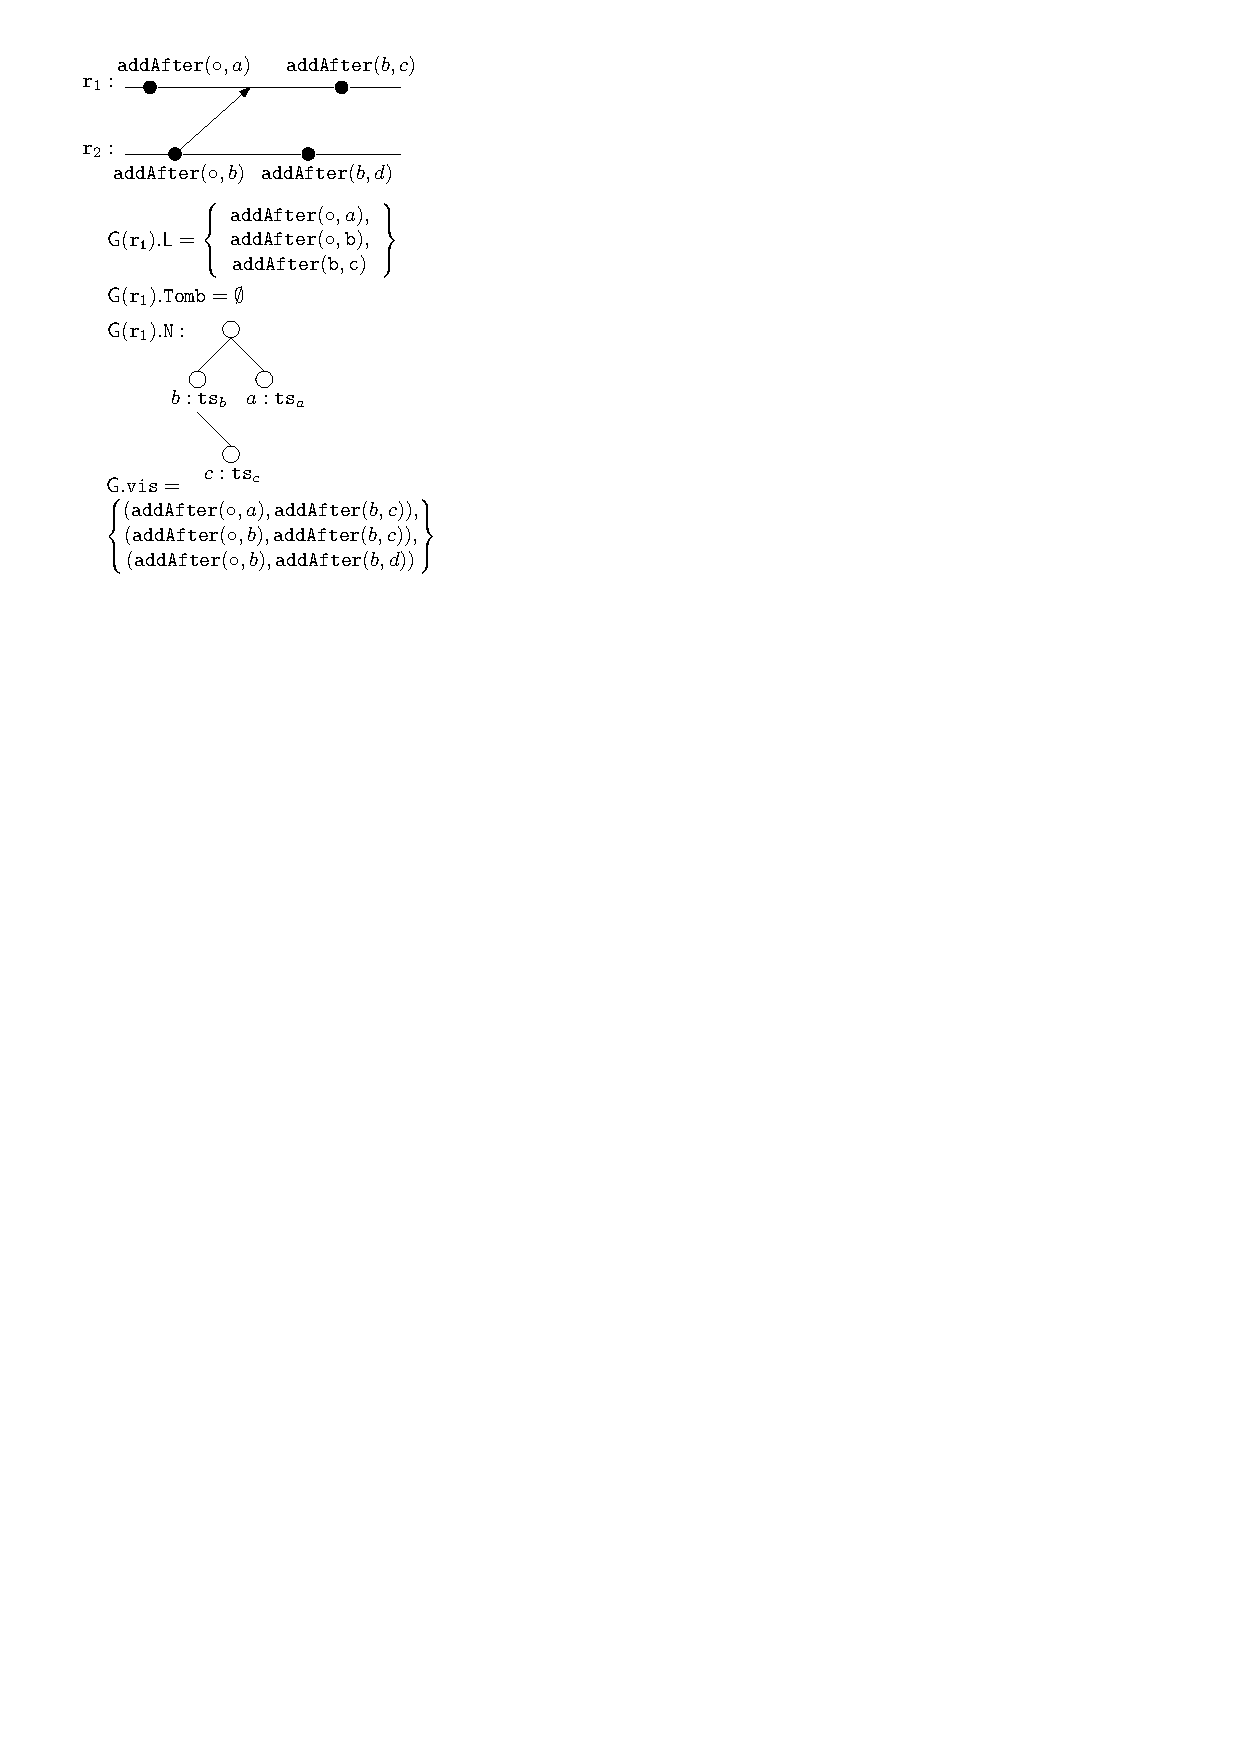
\includegraphics[scale=.7]{figures/LinRGA-1}
      \vspace{1.3cm}
    \caption{}
    \label{fig:rga-sem-1}
  \end{subfigure}
  \begin{subfigure}[!ht]{.3\linewidth}
      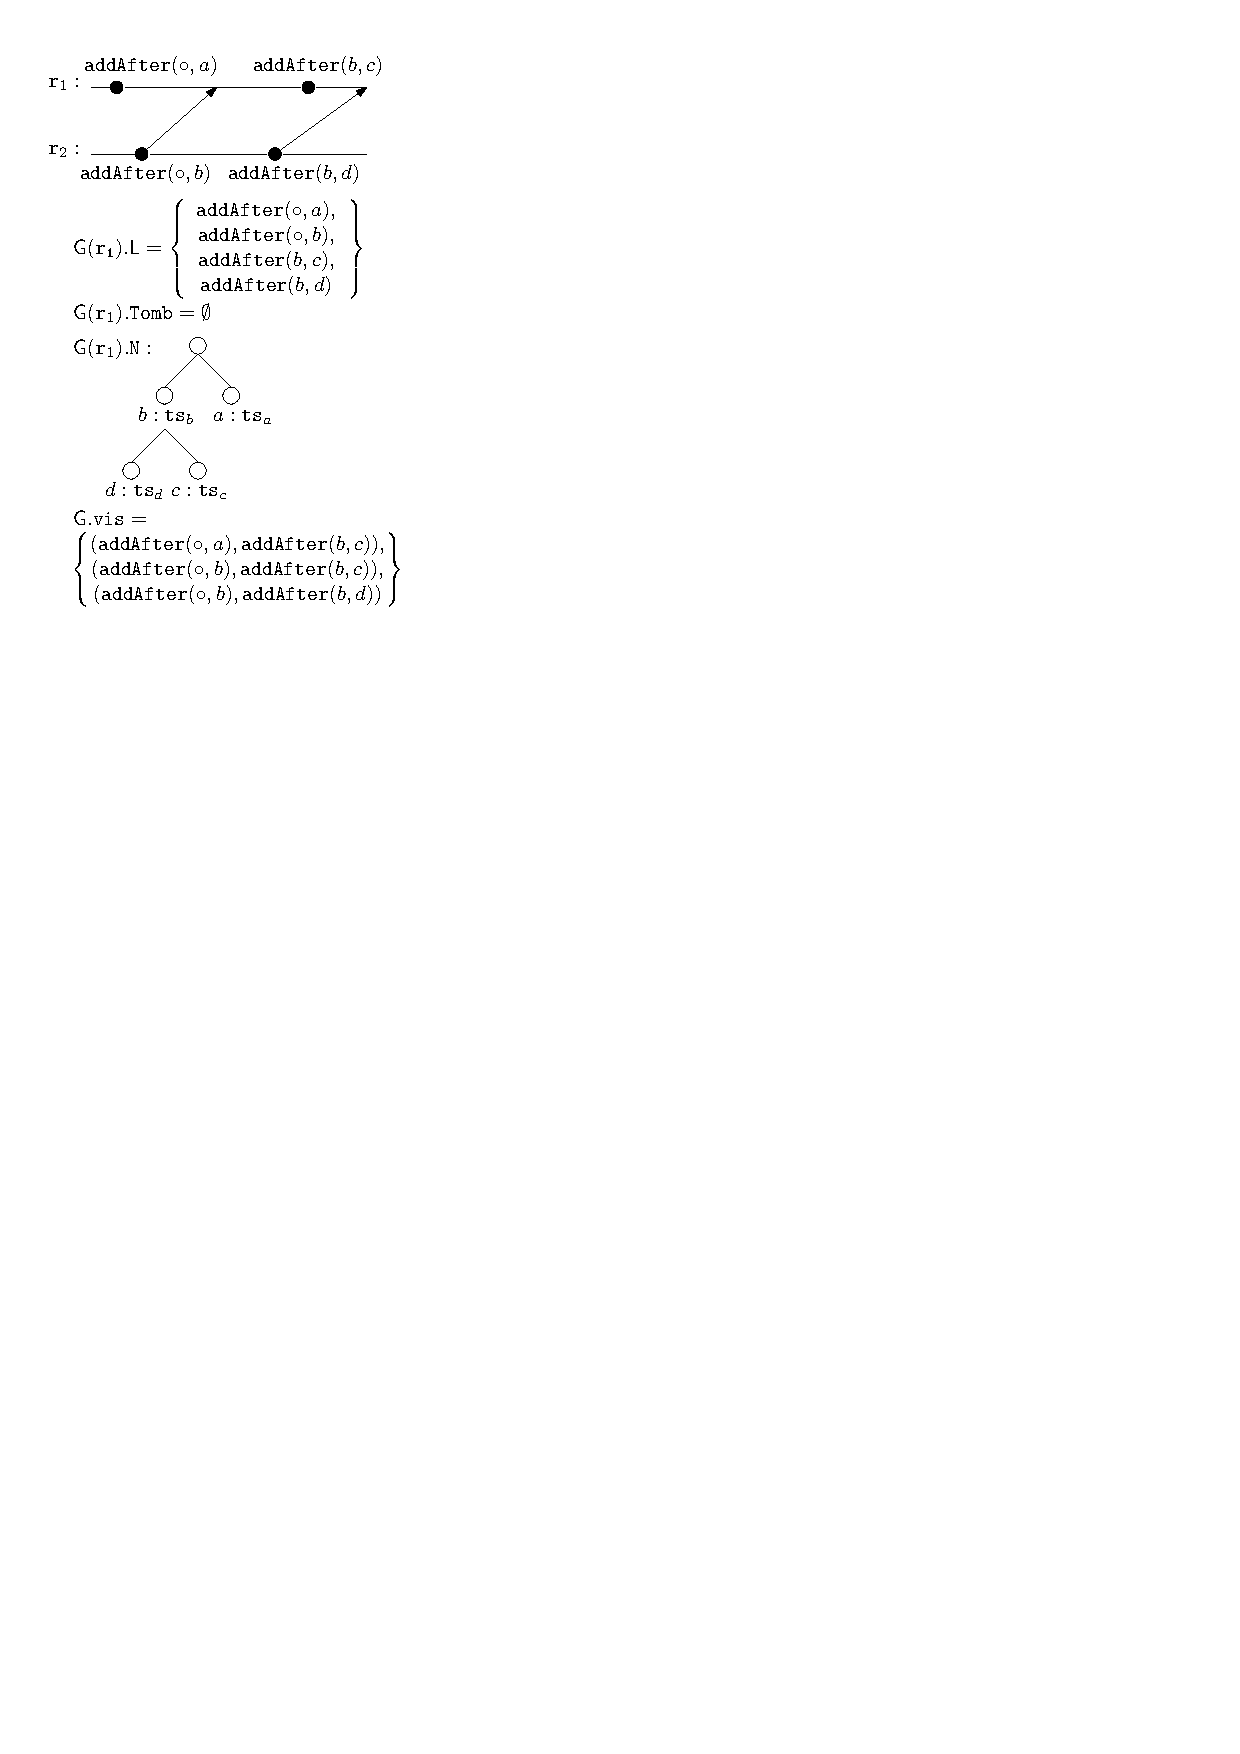
\includegraphics[scale=.7]{figures/LinRGA-2}
      \vspace{1cm}
    \caption{}
    \label{fig:rga-sem-2}
  \end{subfigure}
  \begin{subfigure}[!ht]{.3\linewidth}
    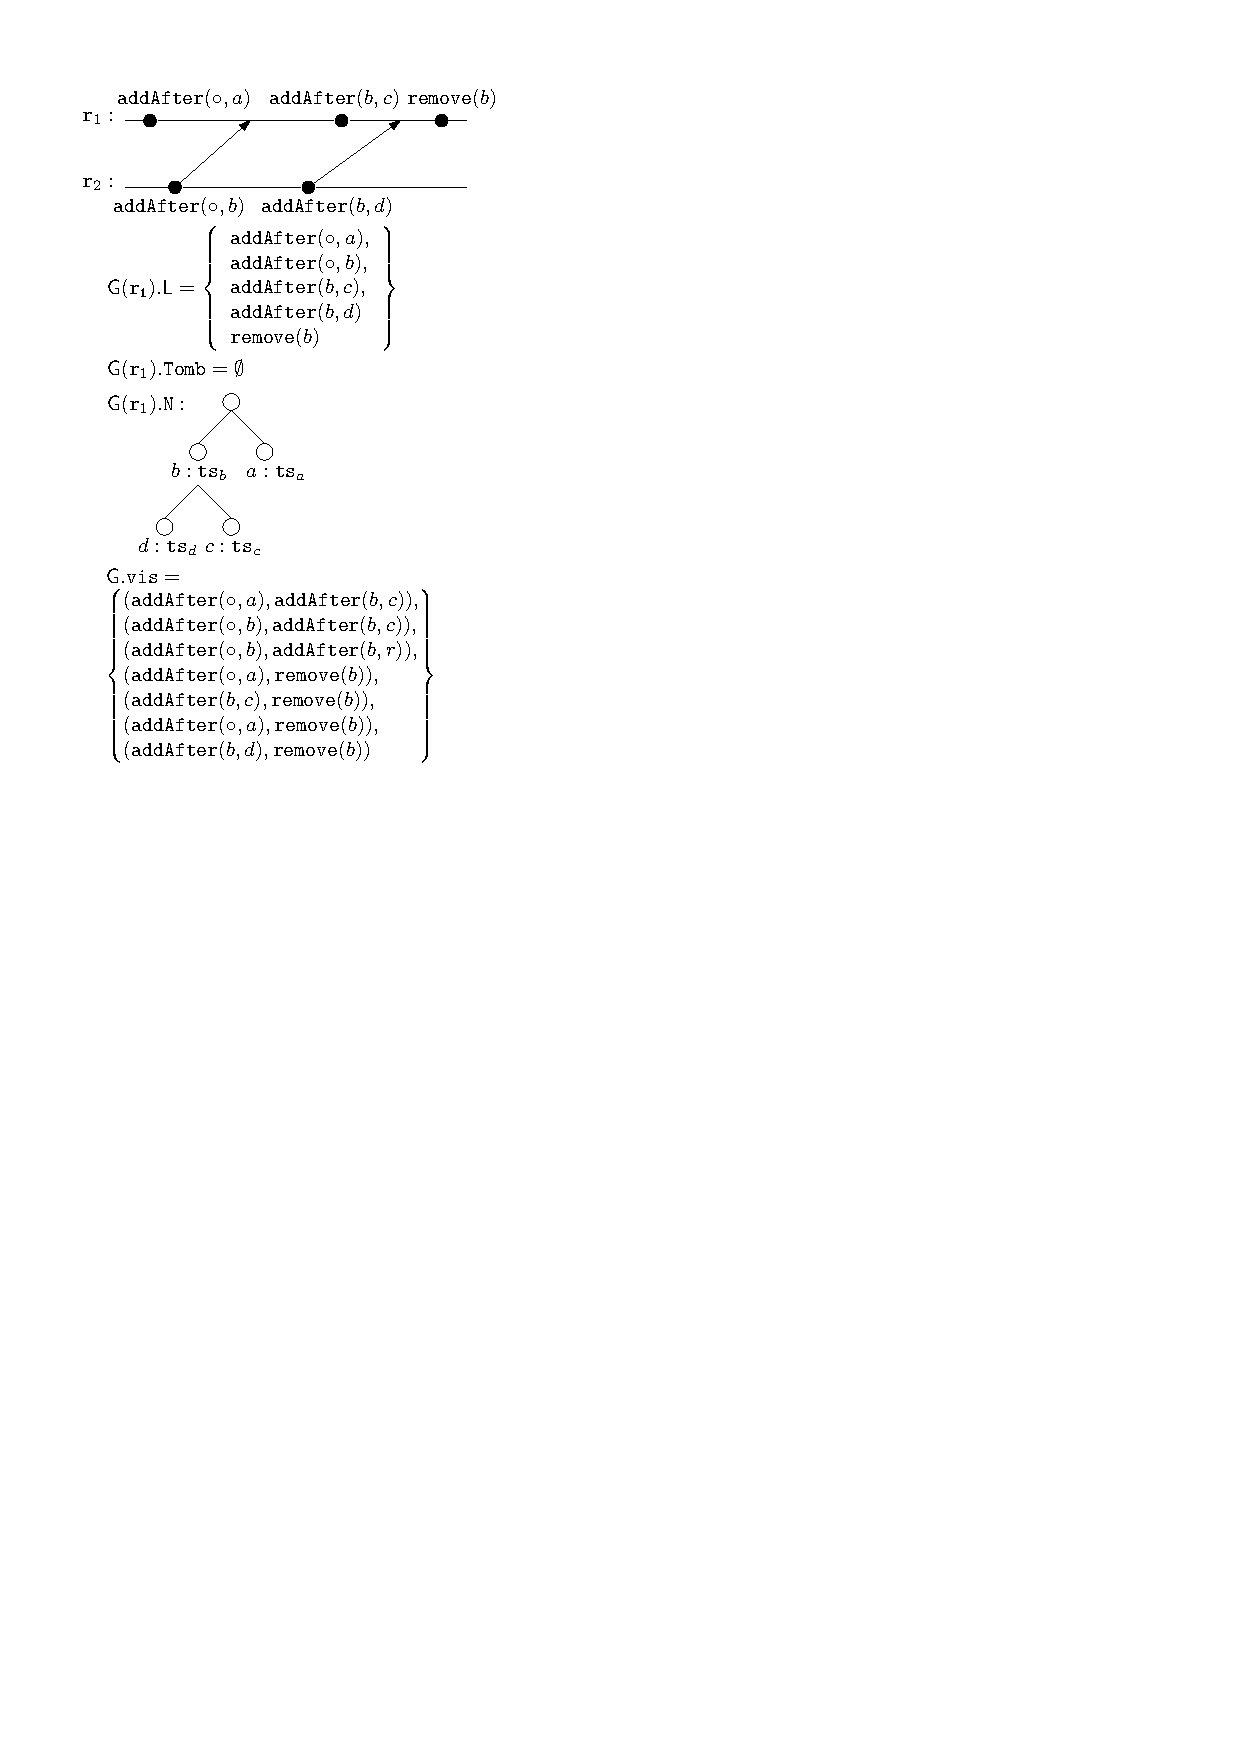
\includegraphics[scale=.7]{figures/LinRGA-3}
    \caption{}
    \label{fig:rga-sem-3}
  \end{subfigure}
  \caption{Example of the semantics of RGA }
  \label{fig:rga-sem}
\end{figure}

In the sequel it will be useful to distinguish query (or pure) methods
which do not modify the state from state-modifying methods, which we
shall call updates (or effectful).
%
We say that a method $\amethod\in\methods$ of object $\aobj\in \objs$
is a \emph{query} if it always results (by applying the {\tt atSource}
function $\atsource$) in an identity downstream $\effector$ (i.e.
$\delta(\sigma)=\sigma$ for all replica states
$\sigma$).\footnote{While we could have defined a semantics in which a
  read-only operation doesn't generate any downstream, we have preferred
  the current version for uniformity.}
We shall call an \emph{update} to any method $\amethod$ which is not a
query -- that is, whose effectors are not the identity function -- and
whose resulting downstream and return value do not depend on the
initial state $\astate$ of the origin replica.
That is, it's behavior is fully determined by its arguments.
More formally, assuming a functional equivalence relation $\equiv$
between downstreams that relates any two downstreams that have the same
effect (modulo the values of timestamps or unique identifiers)
$\amethod$ is called an update when
$\atsource(\sigma,\amethod,\argv)|_2 \equiv
\atsource(\sigma',\amethod,\argv)|_2$, for every $\argv\in\datadomain$
and two states $\sigma,\sigma'\in\Sigma$ (for a tuple $x$, $x|_k$
denotes the projection of $x$ on the $k$-th component).
A method $\amethod$ which is not a query nor an update is called a
\emph{query-update} (it generates a downstream which is not the
identity function, and whose effect depends on the local state of the
replica at which the invocation of $\amethod$ originated).
We denote by $\queries$, $\updates$, and $\queryupdates$, the sets of
operation labels $\alabelobjind{\argv}{\retv}{i,\ats}$ where $\amethod$
is a query, an update, or query-update respectively.
We shall call them query, update, and query-update labels,
respectively.
\fxwarning[nomargin, inline]{EXAMPLES OF QUERIES, UPDATES,
  QUERY-UPDATES.
  PROBABLY DISCUSSED ALREADY ALSO IN THE OVERVIEW.}

%Executions of an object $\aobj$ are defined as usual (as sequences of transitions in $\rightarrow$).
An execution of the object $\aobj$ is a sequence of transitions $\aglobalstate_0\xrightarrow{\aact_0}\aglobalstate_1\xrightarrow{\aact_1}\ldots$.
A \emph{trace} $\atrace$ is the sequence of actions $\aact_0\aact_1\ldots$ labeling the transitions of an execution.
The set of traces of an object $\aobj$ is denoted by $\traces(\aobj)$.
A \emph{history} is a pair $(\alabelset,\avisord)$ where
$\avisord\subseteq \alabelset\times\alabelset$ is an acyclic relation over the set of labels $\alabelset$.
% strict partial
%order over the set of labels $\alabelset$.
Given an execution $e$ ending in a global configuration $(\gstates,
\avisord, \downstreams)$, the \emph{history} of $e$, denoted by $\hist{e}$, is the pair
$(\labeldom{\avisord}, \avisord)$. Note that the relation $\avisord$ is a strict partial order in this case.
We will later allow a more general notion of history in order to deal
with object compositions (see Section~\ref{sec:compositionality}).
Also, the history of a trace $\atrace$, denoted by $\hist{\atrace}$,
is the history of the execution that corresponds to $\atrace$.
The set of histories $\histories(\aobj)$ of an object $\aobj$ is the
set of histories $h$ of an execution $e$ of $\aobj$.

\fxwarning[nomargin, inline]{EXAMPLE OF HISTORY OF AN EXECUTION.} {\color {red} CW: \figurename~\ref{fig:an example run of semantics} shows two steps of a history of RGA, and we can see how history grow in this example. Do I need to draw another figure start from initial global configuration?}

%\ce{Need to talk about read/updates}
%
%Without loss of generality we will consider that the methods in $\mathbb{M}$ can be separated in two disjoint sets of methods: $\mathbb{Q}$ query methods that has no influence on the ``abstract state'' and normally returns an observation of the ``abstract state'' , and $\mathbb{U}$ update methods that has influence on the ``abstract state''.

%
%A sequence $\aexec$ of operation labels is an execution of $\llbracket \aobj \rrbracket$, if there exists a global configuration $\aglobalstate = (\gstates, \avisord, \downstreams)$, such that $\aglobalstate_0 {\xrightarrow{ l }} \aglobalstate$. The history of $\aexec$ is a tuple $(\alabelset, \avisord)$, where $\alabelset$ is the set of labels of $l$. Let $\mathit{history}(\llbracket \aobj \rrbracket)$ be the set of histories of all executions of $\llbracket \aobj \rrbracket$. Then, $\aobj$ is \crdtlinearizable{}, if each of its history is, as stated by the following:
%
%
%
%\begin{definition}[Correctness of a CRDT Object]
%\label{definition:correctness of a CRDT object}
%A CRDT object $\aobj$ is \crdtlinearizable{} w.r.t a sequential specification \Spec{}, if each history of $\mathit{history}(\llbracket \aobj \rrbracket)$ is \crdtlinearizable{} w.r.t \Spec{}.
%\end{definition}
%

%\subsection{Histories}
%
%
%Firstly we will introduce the notion of \emph{histories} to represent
%abstractly the execution of a concrete client operating on an
%implementation of the data structure.
%
%Histories are composed of operation labels.
%We can now define execution \emph{histories}.
%
%\gpnote[nomargin, inline]{Maybe we have an overlap of IDs}
%% We assume a set $\aopid \in \opids$ to represent unique \emph{operation identifiers}.
%
%
%\begin{definition}[histories]
%  \label{definition:histories} An execution history is a tuple of the form
%  $(\alabelset, \avisord)$, where
%  \begin{enumerate}
%  \item $\alabelset$ is the set of labels representing the operations of
%    the execution,
%  % \item $\arepord \in (\alabelset \times \alabelset)$ is the
%  %   \emph{replica order}, a binary relation between the labels of the
%  %   execution, such that when restricted to labels of operations generated
%  %   by each single replica it is a total order, and it does not relate labels of
%  %   operations from different replicas, and
%  \item $\avisord \in (\alabelset \times \alabelset)$ is the
%    \emph{visibility order}, an \emph{acyclic partial order}
%    relation between the labels of the execution, such that if $(\alabel,
%    \alabel') \in \avisord$ then the operation corresponding to the label
%    $\alabel'$ witnessed in its execution the effects of the operation
%    with label $\alabel$.
%  \end{enumerate}
%\end{definition}

\subsection{Sequential Specifications}
\label{subsec:sequential specification}

\fxwarning[nomargin, inline]{INTRODUCE THIS SUBSECTION}

%\gp{We should add the specifications (even non-deterministic here.)}
\begin{definition}[Sequential Specification]
  \label{definition:sequential specification} A \emph{sequential
  specification} (specification, for short) $\Spec$ is a set of tuples $(\alabelset, \aseqord)$, where
  $\alabelset$ is a set of labels and
  $\aseqord$ is a sequence including all the labels in $\alabelset$.
\end{definition}

\gp{I'm changing the arrow because we use it in many places.}
To describe sequential specifications in a succinct way we will
provide an operational description.
To that end, we will associate to specifications a notion of abstract
state, which we shall generally denote by $\abstate$ and its domain
shall be denoted by $\abstates$.
Then, to each valid label $\alabel$ we will associate a transition
relation \;$\xrightharpoonup{\alabel}$\; which, given a state and provided
that the label can be applied into that state, produces a new abstract
state.
Hence, we denote by $\abstate \xrightharpoonup{\alabel}  \abstate'$
%$\absopsem{\abstate} = \abstate'$
the fact that the resulting state for label $\alabel$ with initial
abstract state $\abstate$ is $\abstate'$.
%
%To simplify our descriptions, we will use a shortcut notation for
%$\absopsem{\abstate} = \abstate'$ and will write it as:
%\[ \abstate \xrightharpoonup{\alabel}  \abstate' \]
In the specific case where the label $\alabel$ assumes a certain
precondition $\apre$ over the initial abstract state $\abstate$ we
will use Hoare-style preconditions and write
\[ \big(\abstate\ |\ \apre(\abstate)\big) \xrightharpoonup{\alabel}  \abstate' \]

A sequential specification then is the set of labels that are accepted
by the successive application of the transition relation starting from
some given initial state $\abstate_{0}$.

%A label is called \emph{read-only} if it doesn't change the abstract state, and a \emph{modifier} otherwise.
%The set of labels of a specification $\Spec$ is denoted by $\labelsspec\Spec$. The set of read-only, resp., modifier,
%labels of a specification $\Spec$ is denoted by $\labelsspecrd\Spec$, resp., $\labelsspecmod\Spec$.

% \fxwarning[nomargin, inline]{REWORK THESE EXAMPLES. DON'T WE NEED JUST
%   TWO EXAMPLES, RGA AND OR-SET ?}
% \gpnote[nomargin, inline]{Yes, I think so. Though it might be nice to
%   show more specs, since it kinda proves that they are easy to
%   read/write/understand.}

\gpwarning{Lots of rewriting to do here.}

Let us consider the specification of a very counter object, and then
the specifications of the RGA and OR-Set objects described above.

\begin{example}[Sequential Specification of a Counter]
\label{definition:sequential specification of counter}
The sequential specification $\mathit{counter}_s$ of counter is so
that $\abstates = \mathbb{Z}$, that is the state will be an integer,
and the transitions are given as follows:
\[
  \begin{array}[rcl]{rcl}
    k & \xrightharpoonup{\alabellong[\mathsf{inc}]{}{}} & k+1\\
    k & \xrightharpoonup{\alabellong[\mathsf{dec}]{}{}} & k-1\\
    k & \xrightharpoonup{\alabellong[\mathsf{read}]{}{k}} & k
  \end{array}
\]
% \begin{itemize}
% \setlength{\itemsep}{0.5pt}
% \item[-] $k \xrightharpoonup{\alabellong[\mathsf{inc}]{}{}} k+1$
% \item[-] $k \xrightharpoonup{\alabellong[\mathsf{dec}]{}{}} k-1$
% \item[-] $k \xrightharpoonup{\alabellong[\mathsf{read}]{}{k}} k$
% \end{itemize}
\end{example}


\begin{example}[Sequential Specification of RGA-like List
  (with $\mathtt{addAfter}$ method)]
  \label{definition:sequential specification of or-set}
  Each abstract state $\abstate = (l,T)$ contains a sequence $l$ of
  elements of a given type and a set $T$ of elements appearing in the
  list.
  The element $l$ is the list of all input values, whether already
  removed or not; while $T$ stores the removed values and is used as
  \emph{tombstone}.
  The sequential specification \gpnote*{Is this name used
    anywhere?}{$\mathit{listAft}_s$} of list with add-after interface is
  given with the transitions as follows:
  \[
    \begin{array}{rcl}
      \big(\ (l_1 \cdot a_k \cdot l_2,T\big)\ |\ a\text{ is fresh}\ \big)
      & \xrightharpoonup{\alabelshort[\mathtt{addAfter}]{a_k,a}}
      & (l_1 \cdot a_k \cdot a \cdot l_2,T)\\
      \big(\ (l,T)\ |\ a_k\ \text{occurs in}\ l\ \big)
      & \xrightharpoonup{\alabelshort[\mathtt{remove}]{a_k}}
      & (l,T \cup \{a_k\})\\
      (l,T)
      & \xrightharpoonup{\alabellong[\mathtt{read}]{}{s}{}}
      & (l,T)\
        \left[\begin{array}{c}
                 \text{with $s$ is obtained from $l$}\\
                 \text{by removing the values in $T$}
        \end{array}\right]
 \end{array}
  \]

  Method $\alabelshort[\mathtt{addAfter}]{a_k,a}$ puts $a$ immediately
  after $a_k$ in $l$, assuming that each value is put into list at
  most once.
  Method $\alabelshort[\mathtt{remove}]{a_k}$ adds $a_k$ into $T$,
  hence removing $a_k$ from the list for subsequent calls to the
  $\mathtt{read}$ method.
  Thus, $\alabellong[\mathtt{read}]{}{s}{}$ returns the list content
  excluding any element appearing in $T$.
  Assume that the initial value of list is $(\circ,\emptyset)$, and
  $\circ$ is never removed.
  When the context is clear, in $\ensuremath{\tt read}$ operation, we
  will omit $\circ$ in return value.
\end{example}

% {\color {red} CW: The sequential specification of OR-set and list with add-after interface}
\begin{example}[Sequential Specification of OR-Set]
\label{definition:sequential specification of or-set}
The query-update rewriting of OR-set is as follows: $\gamma( \alabelshort[{\tt remove}]{a} ) = ( \alabellong[{\tt readIds}]{a}{S}{}, \alabelshort[{\tt remove}]{a,S})$.


% \gpwarning{I still don't like the pairs for OR-Set}
Each abstract state $\abstate$ is a set of tuples $(a,id)$, where $a$
is a data and $id$ is a identifier. The sequential specification
$\mathit{OR-Set}_s$ of OR-Set is given by the transitions:
\[
  \begin{array}{rcl}
    \abstate
    & \xrightharpoonup{\alabellong[\mathtt{readIds}]{a}{S}{}}
    & \abstate\
      \begin{array}{c}
        [\text{with}\ S = \{ (a,id)\ \vert\ (a,id) \in \abstate\}]
      \end{array}\\
    \abstate &
               \xrightharpoonup{\alabelshort[\mathtt{remove}]{a,S}}
    & \abstate \setminus S \\
    \big(\ \abstate\ |\ \mathtt{id}\ \text{does not occur in } \abstate\ \big)
             & \xrightharpoonup{ \alabelshort[{\tt add}]{a,id} }
    & \abstate \cup \{ (a,\mathtt{id}) \}\\
    \abstate
    & \xrightharpoonup{\alabellong[\mathtt{read}]{a}{ S }{}}
    & \abstate\
      \begin{array}{c}
        [\text{with}\ S = \{ a\ \vert\ \exists\ \mathtt{id}, (a,\mathtt{id}) \in \abstate \}]
      \end{array}
  \end{array}
\]

Here $\alabellong[{\tt readIds}]{a}{S}{}$ returns the set of pairs with data $a$, $\alabelshort[{\tt remove}]{a,S}$ removes $S$ from the abstract state, $\alabelshort[{\tt add}]{a,id}$ puts $\{ (a,id) \}$ into the abstract state, and $\alabellong[{\tt read}]{}{S'}{}$ returns the value of the or-set.
\end{example}

\fxwarning[nomargin, inline]{TALK ABOUT SPECIFICATIONS OF A SET OF OBJECTS, OBTAINED AS A PRODUCT OF PER-OBJECT SPECIFICATIONS.}

\subsection{Definition of \CRDTLin{}}
\label{subsec:definition of distributed linearizability}

We now provide the definition of \crdtlin{} which characterizes histories of CRDT objects.
To simplify the presentation, we consider first the case where all the labels in the history are
either queries or updates (the case of query-updates is considered later in this section).
%
%To simplify the argument we will assume for the time being that all
%labels in a specification can be classified into update labels
%$\alabel_{up} \in \Updates$ and into $\alabel_{qr} \in \Queries$.
%Later we will extend the framework to consider query/update
%operations.
%
%We will generally assume that methods are predefined as either update
%or query, and labels are defined according to the method.
%In general however, given a specification in the operational style
%described above, we can identify a label as an update if in its
%specification the state before and after are different.
%Formally, if $\abstate \xrightarrow{\alabel} \abstate'$ belongs to $\Spec$
%and $\abstate \neq \abstate'$ we say that $\alabel$ is an update, and
%$\alabel \in \Updates$.\footnote{We assume that labels are
%  consistently update or query, should there be labels acting sometimes
%  as update and sometimes as only query, a simple renaming would suffice
%  to distinguish them.}
%A label is said to be a query if it is not an update.
%We will later add an additional case for query/update labels.
%
The intuition of our notion of \crdtlin{} is that there is a \emph{global} sequence
(or linearization) of the update operations in an execution which can
produce the state of \emph{each} replica when \emph{all} the updates are visible to them.
In intermediate steps, any replica state should be the result of applying a subsequence of updates
of this global sequence. This is because our semantical model allows replicas to see a subset of the updates
performed up to some moment.
%``explains'' the states of each replica,
%i.e., any state observed by any replica should be the result of applying a subsequence of updates
%in this sequence, and eventually, when all the updates are delivered at a replica~\footnote{Their corresponding downstreams are executed on that replica.}, its state is the result of applying this sequence of updates.
%%for update
%%operations there is a global linear sequence (or history) which can
%%produce the final state obtained by the execution.
%%In other words, any state observed by any replica should be the result
%%of a prefix of this sequential history.
%This notion is akin to Linearizability~\cite{HerlihyW90} when
%constrained to update-only operations.
%Evidently, this notion does not extend to query operations, since in
%our semantical model replicas can see a subset of the global updates
%performed at any moment, then we must allow for queries to read a
%sub-sequence of the updates in the global sequence mentioned above.
Therefore, each query should be justified by considering the
sub-sequence of the global sequence restricted to the updates that are
visible to that query.
To be precise:
%\gpnote*{We consider single-object only in this section} {A history is
%  single-object, if it contains operations of a single object.
%  A history is multi-object, if it contains operations of multiple
%  objects.}
%In the following we propose distributed linearizability for histories.
%\gpwarning*{}{We have to say that we distinguish query and update
%  labels, perhaps define formally (for queries the visibility is
%  important, updates change the state, but the visibility might not be
%  important.)}
%
%Before defining $\crdtlin{}$ it will be useful to present a definition
%of linearizability as given by Herlihy and Wing~\cite{HerlihyW90} but
%specialized for our notion of histories.
%We shall call this notion \HWLin{}.
%
%\begin{definition}[\HWLin{}]
%  A history $h = (\alabelset,\avisord)$ is related by \HWLin{}
%  w.r.t.
%  a sequential specification \Spec{}, if there exists a specification
%  history $(\alabelset, \aseqord) \in \Spec$,
%  called the \hwlinearization{} of $h$, where we require that $\aseqord$ be
%  consistent with $\avisord$ (i.e.
%  $(\aseqord \cup \avisord)^+$ is acyclic).
%  % Notice that this means that the visibility of operations in the
%  % \hwlinear{} history is exactly the prefix in $\aseqord$ up to that
%  % operation.
%\end{definition}
%
%This notion is too strong in general as we have shown in the examples
%of~\autoref{sec:CRDT implementations}.
%We shall relax this definition to accept histories where
%not all operations are seen by every query.
%
\begin{definition}
  \label{definition:ralinearizability1} A history $h =
  (\alabelset,\avisord)$ with $\alabelset\subseteq \queries\uplus\updates$ is \crdtlinearizable{} w.r.t. a
   sequential specification
%\gpnote*{First mention?}{deterministic}
  \Spec{}, if there exists a specification sequence
  $(\alabelset, \aseqord) \in \Spec{}$, called the
  \emph{\crdtlinearization{}} of $h$ -- where we remark that the set of labels
  are identical -- such that %
  % \gpwarning*{}{This definition has to be worked out again}
  \begin{enumerate}[(i)]
  \item \aseqord{} is consistent with  \avisord{}, that is: $(\avisord
    \cup \aseqord)^{+}$ is acyclic,
  \item the projection of $\aseqord$ to \emph{updates} is
    admitted by $\Spec$, i.e.
    $\aseqord\!\downarrow_{\updates} \in \Spec$, where we denote by
    $\aseqord\downarrow_{S}$ the restriction of the order $\aseqord$ to
    the set $S$, and
  \item for each query $\alabel_{\mathsf{qr}}\in \alabelset$, the subsequence of updates visible to $\alabel_{\mathsf{qr}}$ together with $\alabel_{\mathsf{qr}}$ is itself admitted by $\Spec$, i.e., $\aseqord\!\downarrow_{\avisord^{-1}(\alabel_{\mathsf{qr}})\cap \updates}\!\cdot\
    \alabel_{\mathsf{qr}} \in \Spec$.
\end{enumerate}
In this case we say that $(\alabelset, \aseqord)$ is an \emph{\crdtlinearization{}} of $h$ w.r.t. $\Spec{}$.
\end{definition}

In a nutshell, this definition requires that for a given
history, there exists a specification sequence such
that
\begin{inparaenum}[(i)]
\item the set of labels are the same and the order in the sequence is
  consistent with the visibility order of the history, that
\item when restricted to update operations -- that is all the updates --, the sequence belongs to
  the specification, and that
\item every query operations can be justified by the specification based only
  on the updates that precede it in the sequence and that are visible
  to it.
\end{inparaenum}

\fxwarning[nomargin, inline]{REFER TO AN EXAMPLE FROM THE OVERVIEW} {\color {red}CW: \figurename~\ref{fig:a history of RGA and its RA-linearization} gives a history of RGA and its linearization step by step.}

We now consider the case where histories include query-updates.
In such a case, we apply~\autoref{definition:ralinearizability1} on a
rewriting of the original history where each query-update is
decomposed into a label representing the query part and another label
representing the update part.
\gpnote*{Clarify this sentence. Not clear where the new labels come from}
{This rewriting may introduce new labels, which do not correspond to
original operations of the data type, but which have been extended to
be taken into account by the specification.
Also, other (update) operations of the object may be rewritten as
well.}
\fxwarning[nomargin, inline]{EXPLAIN THE OR-SET CASE.} {\color {red}CW: \figurename~\ref{fig:a history of OR-set, its update-query rewriting, and its RA-linearization} gives a history of OR-set, its query-update rewriting, and its \crdtlinearization{}.}

TODO MODIFY $\gamma$ BECAUSE IT MAY REWRITE UPDATES AS WELL. DO WE NEED TO REWRITE QUERIES ?

A mapping $\gamma:\labels\rightarrow \labels^{\leq 2}$, where $\labels^{\leq 2}$ is the set of labels and pairs of labels in $\labels$, is called a \emph{query-update rewriting}.
%Labels mapped by $\gamma$ to singletons preserve their query or update status
We assume that every query or update label is mapped by $\gamma$ to a singleton and that the $\gamma$ image of such a label preserves its status, i.e., $\gamma(\alabel)$ is a query, resp., update, whenever $\alabel$ is a query, resp., update. Also, query-updates labels $\alabel$ are mapped to pairs $\gamma(\alabel)=(\alabel_1,\alabel_2)$ where $\alabel_1$ is a query and $\alabel_2$ is an update. These assumptions are important when applying~\autoref{definition:ralinearizability1} on the rewriting of a history, since this definition relies on a partitioning of the labels into queries and updates.
%We say that $\gamma$ is \emph{consistent} with $\Spec$ when $\mathsf{image}(\gamma)\subseteq \labelsspec\Spec^{\leq 2}$ and for every label $\alabel$, if $\gamma(\alabel)=(\alabel_1,\alabel_2)$ then $\alabel_1$ is read-only and $\alabel_2$ is a modifier (of $\Spec$).
%For $\alabel\in \queryupdates$ and $\gamma(\alabel)=(\alabel_1,\alabel_2)$, the label $\alabel_1$ is considered a query and $\alabel_2$ an update.
For a history $h=(\alabelset,\avisord)$, its $\gamma$-rewriting is a
history $\gamma(h)=(\alabelset',\avisord')$ where
\begin{itemize}
\item $\alabelset'$ is obtained by replacing each label $\alabel$ in
  $\alabelset$ with $\gamma(\alabel)$ (a label may be replaced by two
  labels),
\item whenever a (query-update) label $\alabel$ is mapped by $\gamma$
  to a pair $(\alabel_1,\alabel_2)$ (i.e.
  $\gamma(\alabel)=(\alabel_1,\alabel_2)$), we have that the query is
  ordered before the update, formally $(\alabel_1,\alabel_2)\in \avisord'$,
\item $\avisord'$ preserves the order between labels which are
  mapped to singletons, and
  % whenever two labels are ordered by $\avisord$ and they are mapped
  % by $\gamma$ to singletons, then their $\gamma$-images remain
  % ordered in $\avisord'$. Similarly,
  for any query-update label $\alabel$ mapped to a pair
 $(\alabel_1,\alabel_2)$, the query $\alabel_1$ sees exactly the same
 set of operations as $\alabel$ and any operation which saw $\alabel$
 must see $\alabel_2$.
 Formally, whenever $(\alabel,\alabel')\in\avisord$ we have that
 $(\secondrep(\gamma(\alabel)),
 \firstrep(\gamma(\alabel')))\in\avisord'$, where for a label $\alabel$,
 $\firstrep(\gamma(\alabel))$ (resp., $\secondrep(\gamma(\alabel))$), is
 $\gamma(\alabel)$ when $\gamma(\alabel)$ is a singleton, or its first (resp.,
 second) projection when $\gamma(\alabel)$ is a pair.
\end{itemize}
The following definition
extends~\autoref{definition:ralinearizability1} to arbitrary histories
using the rewriting defined above.
% \gpnote[nomargin, inline]{I'd probably use $\Pi^*_i$ for the i-th
%   projection of a tuple, or the singleton.}

\begin{definition}[\CRDTLin{}]
  \label{definition:distributed linearizability} A history $h =
  (\alabelset,\avisord)$ is \crdtlinearizable{} w.r.t. a
   sequential specification
%\gpnote*{First mention?}{deterministic}
  \Spec{}, if there exists a query-update rewriting $\gamma$ such that $\gamma(h)$ is \crdtlinearizable{} w.r.t. \Spec{}.
\end{definition}


A set $H$ of histories is called \crdtlinearizable{} w.r.t a
sequential specification $\Spec$ when each history $h\in H$ is
\crdtlinearizable{} w.r.t.
$\Spec$.
A data type implementation is \crdtlinearizable{} w.r.t.
$\Spec$ if for any object $\aobj$ of the data type, the set
$\histories(\aobj)$ is linearizable w.r.t. $\Spec$.


\fxwarning[nomargin, inline]{MOVE THE FOLLOWING WHEN WE NEED IT (WHEN WE TALK ABOUT SOME NONDETERMINISTIC SPECIFICATION, E.G., WOOT)}

An important property of CRDT algorithms is \emph{convergence}.
Convergence means that all replicas will arrive to the same final
state when the same set of operations are applied to them.
For the moment we concentrate on specifications that are
\emph{deterministic}.
That is to say that for every label, the transition from a given
initial state can produce at most one final state.
We will later remove this restriction.
It is useful to remark that if the specification of a CRDT is
deterministic, then our definition of \crdtlin{} implies the
convergence of the data type, as formalized in the following lemma.

\begin{lemma}
\label{lemma:distributed linarizability implies convergence}
If a history $h$ is \crdtlinearizable{} w.r.t. a deterministic
sequential specification \Spec, then $h$ is convergent.
\end{lemma}









\forget{
\fxfatal[nomargin, inline]{Complete the others!}
\begin{example}[sequential specification of multi-value register]
\label{def:spec-MVR}
The sequential specification $\mathit{MVReg}_s$ of multi-value
register is given as follows: Let $\mathit{state}$ be a set and each
its element $(a,\mathit{id},f)$ is a tuple of a data $a$, an
identifier $\mathit{id} \in \mathbb{O}$, and a flag $f \in \{
\mathit{true},\mathit{false} \}$.
\begin{itemize}
\setlength{\itemsep}{0.5pt}
\item[-] $\{ \mathit{state} = S \}$ $(write(a),\mathit{id},S_1)$ $\{
  \mathit{state} = S[(b,\mathit{id}_1) \in S_2 : \mathit{false}] \cup
  \{ (a,id,\mathit{true}) \} \}$. Here $S_2 = \{ (b,\mathit{id}_1)
  \vert (b,\mathit{id}_1,\mathit{true}) \in S \wedge id \in S_1 \}$.
\item[-] $\{ \mathit{state} = S \wedge S_1 = \{ a \vert
  (a,\_,\mathit{true}) \in S \} \}$ $read() \Rightarrow S_1$ $\{
  \mathit{state} = S \}$.
\end{itemize}
\end{example}

\begin{example}[set and its sequential specification]
\label{definition:sequential specification of set}
A set has three methods: $\mathit{add}(a)$ inserts item $a$ into set;
$\mathit{rem}(a)$ removes $a$ from set; and $\mathit{read}$ returns
the set content.
% It implicitly assumes that each item being put into the set only
% once.
% Here we assume that when a item is removed, it will never be added
% again.
Here we assume that $\mathit{rem}$ will also be checked for
visibility.
The sequential specification $\mathit{set}_s$ of set is given as
follows:  Let $\mathit{state}$ be a set and each its element $(a,f)$
is a tuple of a data $a$ and a flag $f \in \{ \mathit{true},\mathit{false} \}$.
\begin{itemize}
\setlength{\itemsep}{0.5pt}
\item[-] $\{ \mathit{state} = S \wedge (a,\_) \notin S \}$
  $(\mathit{add}(a),\mathit{id})$ $\{ \mathit{state} = S \cup \{
  (a,\mathit{true}) \} \}$.
\item[-] $\{ \mathit{state} = S \wedge (a,\_) \in S \}$
  $(\mathit{add}(a),\mathit{id})$ $\{ \mathit{state} = S \}$.
\item[-] $\{ \mathit{state} = S \wedge (a,\_) \in S \}$
  $(\mathit{rem}(a))$ $\{ \mathit{state} = S[a: \mathit{false} \}$.
\item[-] $\{ \mathit{state} = S \wedge S_1 = \{a \vert
  (a,\mathit{true}) \in S \} \}$ $(\mathit{read}() \Rightarrow S_1)$
  $\{ \mathit{state} = S \}$.
\end{itemize}
\end{example}

%TODO TO MAKE IT MORE INTERESTING I ASSUME THAT REMOVE HAS A PRECONDITION: THE PAIRS REMOVED BY A REMOVE HAVE BEEN ADDED BEFORE

\begin{example}[OR-set and its sequential specification]
\label{def:specification-ORS}
OR-set is essential a multi-set: $\mathit{add}(a)$ inserts an item $a$
into multi-set; $\mathit{rem}(a)$ cancels only items $a$ that are
inserted by $\mathit{add}(a)$ operations visible to this remove
operation; $\mathit{read}$ returns the set of items in multi-set. A
value can be inserted multiple times.

The sequential specification $\mathit{OR}$-$\mathit{set}_s$ of OR-set
is given as follows: Let $\mathit{state}$ be a set and each its
element $(a,\mathit{id},f)$ is a tuple of a data $a$, an identifier
$\mathit{id}$, and a flag $f \in \{ \mathit{true},\mathit{false} \}$.
% In $((rem(a),\mathit{id}'),S_1)$, $S_1$ represents the operations
% visible to this remove operation.
\begin{itemize}
\setlength{\itemsep}{0.5pt}
\item[-] $\{ \mathit{state} = S  \wedge (\_,\mathit{id},\_) \notin S
  \}$ $(\mathit{add}(a),\mathit{id})$ $\{ \mathit{state} = S \cup \{
  (a,\mathit{id},\mathit{true}) \} \}$.
\item[-] $\{ \mathit{state} = S \wedge S_1 = \{ a \vert
  (a,\_,\mathit{true}) \in S \} \}$ $(\mathit{read}() \Rightarrow
  S_1)$ $\{ \mathit{state} = S \}$.
\item[-] $\{ \mathit{state} = S \wedge (a,\_,\_) \in S\}$
  $(rem(a),S_1)$ $\{ \mathit{state} = S[(a,\mathit{id}_1) \in S_2 :
  \mathit{false}] \}$. Here $S_2 = \{ (a,\mathit{id}_1) \vert
  (a,\mathit{id}_1,\mathit{true}) \in S \wedge id \in S_1 \}$.
\end{itemize}
\end{example}


\begin{example}[register and its sequential specification]
\label{def:spec-register}
A register has two methods: $\mathit{write}(a)$ writes $a$ into
register; $\mathit{read}$ returns the value of register. The
sequential specification $\mathit{reg}_s$ of register is given as
follows: Let $\mathit{state} \in \mathbb{D}$ be a value.
\begin{itemize}
\setlength{\itemsep}{0.5pt}
\item[-] $\{ \mathit{state} = a  \}$ $\mathit{write}(b)$ $\{
  \mathit{state} = b \}$.
\item[-] $\{ \mathit{state} = a \}$ $(\mathit{read}() \Rightarrow a)$
  $\{ \mathit{state} = a \}$.
\end{itemize}
\end{example}


\begin{example}[List with add-after interface]
\label{definition:spec-list-add-after}
Assume each item of the list is unique. A list has three methods:
$\mathit{add}(b,a)$ inserts item $b$ into the list at the position
immediately after that of item $a$; $\mathit{rem}(a)$ removes item $a$
from the list; and $\mathit{read}$ returns the list content. We assume
that the initial value of list is $(\circ,\mathit{true})$ and this
node can not be removed. We use the word ``add-after'' to emphasize
the method $\mathit{add}(b,a)$, which is different from the other list
interface that uses method $\mathit{add}(b,a,c)$.

The sequential specification $\mathit{list}_s^{\mathit{af}}$ of list
is given as follows: Let $\mathit{state}$ be a sequence, where each
item is a tuple $(a,\mathit{id},f)$ with data $a$, identifier
$\mathit{id}$ and flag $f \in \{ \mathit{true},\mathit{false} \}$.
Here $\mathit{af}$ represents add-after, and we use $l \uparrow_{S}$
to represent the projection of sequence $l$ into set $S$.
\begin{itemize}
\setlength{\itemsep}{0.5pt}
\item[-] $\{ \mathit{state} = (a_1,\mathit{id}_1,f_1) \cdot \ldots
  \cdot (a_n,\mathit{id}_n,f_n) \wedge k \leq n \wedge b \notin \{
  a_1, \ldots, a_n \} \wedge \mathit{id}_k \in S_1 \}$
  $(add(b,a_k),\mathit{id},S_1)$ $\{ \mathit{state} =
  (a_1,\mathit{id}_1,f_1) \cdot \ldots \cdot (a_k,\mathit{id}_k,f_k)
  \cdot (b,\mathit{id},\mathit{true}) \cdot
  (a_{k+1},\mathit{id}_{k+1},f_{k+1}) \cdot \ldots \cdot
  (a_n,\mathit{id}_n,f_n) \}$.
\item[-] $\{ \mathit{state} = (a_1,\mathit{id}_1,f_1) \cdot \ldots
  \cdot (a_n,\mathit{id}_n,f_n) \wedge k \leq n \wedge \mathit{id}_k
  \in S_1 \}$ $(rem(a_k),S_1)$ $\{ \mathit{state} =
  (a_1,\mathit{id}_1,f_1) \cdot \ldots \cdot
  (a_k,\mathit{id}_k,\mathit{false}) \cdot \ldots \cdot
  (a_n,\mathit{id}_n,f_n) \}$.
\item[-] $\{ \mathit{state} = (a_1,\mathit{id}_1,f_1) \cdot \ldots
  \cdot (a_n,\mathit{id}_n,f_n) \wedge S = \{ a \vert
  (a,\_,\mathit{true}) \in \mathit{state} \} \wedge l = a_1 \cdot
  \ldots \cdot a_n \uparrow_{S} \}$ $(read() \Rightarrow l)$ $\{
  \mathit{state} = (a_1,\mathit{id}_1,f_1) \cdot \ldots \cdot
  (a_n,\mathit{id}_n,f_n) \}$.
\end{itemize}
When the context is clear, in $\mathit{read}$ operation, we will omit
$\circ$.
\end{example}
}
%%% Local Variables:
%%% mode: latex
%%% TeX-master: "draft"
%%% End:


%%!TEX root = draft.tex
%\newcommand{\seqPQ}{\mathsf{SeqPQ}}

\section{CRDT Implementation Correctness}
\label{sec:CRDT implementation semantics and correctness}

In this section, we propose the semantics of CRDT implementations. Based on our definition, we can extract histories from an execution. Then we define the correctness of an CRDT implementation. 



%\subsection{Semantics of Single Object}
%\label{subsec:semantics of single object}

CRDT implementations assume the following two guarantees of downstream:

\begin{itemize}
\setlength{\itemsep}{0.5pt}
\item[-] The downstream of each operation is applied at most once for each replica. 
\item[-] Assume the downstream of operation $\aop_1$ is applied in replica of $\aop_2$ before $\aop_2$ happens. Then, for each replica $\arep$, the downstream of $\aop_2$ can be applied only if the downstream of $\aop_1$ has already been applied. 
\end{itemize}

Given a CRDT object $\aobj$, its semantics is defined as a transition system $\llbracket \aobj \rrbracket_{\mathit{op}} = (\mathit{Config},\mathit{config}_0,\Sigma',\rightarrow)$ as in \figurename~\ref{fig:crdt-opsem}.
 


%\gpfatal[nomargin, inline]{remove if we decide to keep the other semantics}

\begin{figure}[t]
  \centering

\begin{itemize}
\item $ \Delta : \states \rightarrow \states \ni \effector$ \hspace{\fill} Effector or Downstream
%\item $\semop[]{} : \labels \times \states \rightarrow (\states \rightarrow \states)$ \hspace{\fill} Operational Semantics of a Single Operation (Label)
\item $\localstates : \powerset{\labels} \times \states \ni (\alabelset, \astate)$ \hspace{\fill} Local States
\item $\globalstates : (\reps \rightarrow \localstates) \times \powerset{\labels \times \labels} \times (\labels \rightarrow \Delta) \ni (\gstates, \avisord, \downstreams )$ \hspace{\fill} Global States
\end{itemize}


\[
  \inferrule[\text{\sc Operation}]
  {\gstates(r) = (\alabelset, \astate) \\ \mathit{do}(\sigma,\amethod,\argv,\arep) = (\retv,\effector) \\  \effector(\astate) = \astate' \\ \alabel = \alabellongind{\argv}{\retv}{i} \\ \mathit{unique}(i) }
  {(\gstates, \avisord, \downstreams) \xrightarrow{\alabel} (\gstates[\arep \leftarrow (\alabelset \cup \{\alabel\}, \astate')],
    \avisord \cup (\alabelset \times \{\alabel\}), \downstreams[\alabel \rightarrow \effector])}
\]


\[
  \inferrule[\text{\sc DownStream}]
  {\gstates(r) = (\alabelset, \astate) \\ \alabel \in \mathsf{min}_{\avisord}(\dom{\avisord} / \alabelset) \\
    \downstreams(\alabel)(\astate) = \astate'}
  {(\gstates, \avisord, \downstreams) \xrightarrow{} (\gstates[\arep \leftarrow (\alabelset \cup \{\alabel\}, \astate')], \avisord, \downstreams)}
\]

  \caption{Operational Semantics of CRDTs}
  \label{fig:crdt-opsem}
\end{figure} 

A configuration $(\gstates, \avisord, \downstreams)$ is a snapshot of distributed system. $\gstates \in \reps \rightarrow \localstates$ stores the local configuration of each replica. A local configuration $(\alabelset, \astate)$ contains a local state $\astate$ of $\aobj$ and a set $\alabelset$ of labels: $\alabel \in \alabelset$, if the downstream of $\alabel$ has already been applied in this replica. $\avisord \in \powerset{\labels \times \labels}$ stores the visibility among operations, and $\downstreams$ stores the downstream of operations. 

$\rightarrow \in \globalstates \times \labels \times \globalstates$ is the transition relation. The first rule in \figurename~\ref{fig:crdt-opsem} describes replica $\arep$ performing an operation and (possibly) generate a new downstream. $\mathit{unique}(i)$ ensures that $i$ is a unique identifier, and then $\alabel$ is a unique operation label. A new downstream $\effector$ is generated and applied to replica $\arep$. The set $\alabelset$ and $\avisord$ is updated according to $\alabel$. The second rule describes the downstream of $\alabel$ being applied to replica $\arep$. With $\alabel \in \mathsf{min}_{\avisord}(\dom{\avisord} / \alabelset)$, we always choose a operation $\alabel$ that is minimal among operations whose downstream not applied to replica $\arep$ yet. This satisfies the guarantees of downstream. 


A sequence $l$ of operation labels is an execution of $\llbracket \aobj \rrbracket_{\mathit{op}}$, if there exists configuration $(\gstates, \avisord, \downstreams)$, such that $\mathit{config}_0 {\xrightarrow{ l }} (\gstates, \avisord, \downstreams)$. The history of $l$ is a tuple $(\alabelset, \avisord')$, where $\alabelset$ is the set of labels of $l$ and $\avisord' = \avisord$ is the visibility relation recorded in the configuration along transitions.


%\subsection{Correctness of a Single Object}
%\label{subsec:correctness of a single object}

%Given an execution $l = \alpha_1 \cdot \ldots \cdot \alpha_k$ of $\llbracket \mathit{obj} \rrbracket_{\mathit{op}}$ of CRDT object $\mathit{obj}$, we can associate unique operation identifiers with each action of $l$, and then obtain a corresponding history $\mathit{history}(l) = (\mathit{Op},\mathit{ro},\mathit{vis})$, such that

%\begin{itemize}
%\setlength{\itemsep}{0.5pt}
%\item[-] Each operation in $\mathit{Op}$ is a tuple $(m(a) \Rightarrow b,i,\mathit{obj})$, such that $i$ is the operation identifier of a $\mathit{do}(m,a,b,r)$ action of $l$.

%\item[-] $(o_1,o_2) \in \mathit{ro}$, if they are of same replica, and the index of $o_1$ in $h$ is before that of $o_2$.

%\item[-] $(o_1,o_2) \in \mathit{vis}$, if the action of $o_1$ is $\mathit{send}(\mathit{mid},\_)$, and either the action of $o_2$ is $\mathit{receive}(\mathit{mid},\_)$, or there exists $o_3$, such that the action of $o_3$ is $\mathit{receive}(\mathit{mid},\_)$, and $(o_3,o_2) \in \mathit{ro}$.
%\end{itemize}

Let $\mathit{history}(\llbracket \aobj \rrbracket_{\mathit{op}})$ be the set of histories of all executions of $\llbracket \aobj \rrbracket_{\mathit{op}}$. Then, $\aobj$ is \crdtlinearizable{}, if each of its history is, as stated by the following:

\begin{definition}[Correctness of a CRDT Object]
\label{definition:correctness of a CRDT object}
A CRDT object $\aobj$ is \crdtlinearizable{} w.r.t a sequential specification $\mathit{spec}$, if each history of $\mathit{history}(\llbracket \mathit{obj} \rrbracket_{\mathit{op}})$ is \crdtlinearizable{} w.r.t $\mathit{spec}$.
\end{definition}

















\forget{
In this section, we propose the semantics of %a state-based CRDT or a operation-based CRDT.
CRDT implementations. Then we shows how to extract histories from execution, and the correctness of CRDT implementations.



\subsection{Semantics of a Single Object}
\label{subsec:semantics of a single object}

CRDT implementations assume the following two guarantees of message delivery:

\begin{itemize}
\setlength{\itemsep}{0.5pt}
\item[-] No duplicated delivery: Each message is delivered to a replica at most once.
\item[-] Causal delivery: Given two update operations $o_1$ and $o_2$, and assume $o_1$ is visible to $o_2$. Or we can say, $o_1$ is related to $o_2$ by several times of replica order and message delivery. Then, for each replica, once it receives $o_2$, it must be the case that $o_1$ has been previously received.
\end{itemize}

Given a CRDT object $\mathit{obj}$ with $\Sigma$ be the set of local states, its semantics is defined as $\llbracket \mathit{obj} \rrbracket_{\mathit{op}} = (\mathit{Config},\mathit{config}_0,\Sigma',\rightarrow)$ as in \figurename~\ref{fig:the semantics of a operation-based CRDT object}.


\gpfatal[nomargin, inline]{remove if we decide to keep the other semantics}

\begin{figure}[t]
  \centering

\begin{itemize}
\item $ \Delta : \states \rightarrow \states \ni \effector$ \hspace{\fill} Effector or Downstream
\item $\semop[]{} : \labels \times \states \rightarrow (\states \rightarrow \states)$ \hspace{\fill} Operational Semantics of a Single Operation (Label)
\item $\localstates : \powerset{\labels} \times \states \ni (\alabelset, \astate)$ \hspace{\fill} Local States
\item $\globalstates : (\reps \rightarrow \localstates) \times \powerset{\labels \times \labels} \times (\labels \rightarrow \Delta) \ni (\gstates, \avisord, \downstreams )$ \hspace{\fill} Global States
\end{itemize}


\[
  \inferrule[\text{\sc Operation}]
  {\gstates(r) = (\alabelset, \astate) \\ \semop[\alabel]{\astate} = \effector \\ \effector(\astate) = \astate'}
  {(\gstates, \avisord, \downstreams) \xrightarrow{\alabel} (\gstates[\arep \leftarrow (\alabelset \cup \{\alabel\}, \astate', \downstreams)],
    \avisord \cup (\alabelset \times \{\alabel\}), \downstreams[\alabel \rightarrow \effector])}
\]

\[
  \inferrule[\text{\sc DownStream}]
  {\gstates(r) = (\alabelset, \astate) \\ \alabel \in \mathsf{min}_{\avisord}(\dom{\avisord} / \alabelset) \\
    \downstreams(\alabel)(\astate) = \astate'}
  {(\gstates, \avisord, \downstreams) \xrightarrow{} (\gstates[\arep \leftarrow (\alabelset \cup \{\alabel\}, \astate')], \avisord, \downstreams)}
\]

  \caption{Operational Semantics of CRDTs}
  \label{fig:crdt-opsem}
\end{figure}


\begin{figure}[ht]
$\mathit{RState} = \mathbb{R} \rightarrow \Sigma$

$\mathit{TState} = \mathbb{MID} \times \mathbb{MSG} \times \mathbb{R}$

$\mathit{MsgHB} \subseteq \mathbb{MID} \times \mathbb{MID}$

$\mathit{MsgDel} \subseteq \mathbb{MID} \times \mathbb{R}$

$\mathit{Config} = \mathit{RState} \times \mathit{TState} \times \mathit{MsgHB} \times \mathit{MsgDel}$, $\mathit{config}_0 \in \mathit{Config}$.

$\Sigma' = \mathit{do}(\mathbb{M} \times \mathbb{D} \times \mathbb{D} \times \mathbb{R} \times \mathbb{MID}) \cup \mathit{do}(\mathbb{M} \times \mathbb{D} \times \mathbb{D} \times \mathbb{R}) \cup \mathit{receive}(\mathbb{MID} \times \mathbb{R})$

\begin{itemize}
\setlength{\itemsep}{0.5pt}
\item[] $\begin{array}{l c}
   \bigfrac{
   \begin{array}{c}
     R(r) = \sigma, r.\mathit{do}(\sigma,m,a) = (\sigma',b,\mathit{msg}), \mathit{msg} \neq \emptyset, \mathit{unique}(\mathit{mid}), \\
     S_1 = \{ (\mathit{mid}',\mathit{mid}) \vert (\mathit{mid'},r) \in \mathit{MsgDel} \}, S_2 = \{ (\mathit{mid}',\mathit{mid}) \vert \mathit{mid}' \in T, \mathit{mid}' \ is \ of \ replica \ r \}
   \end{array}}
     {(R,T,\mathit{msgHB},\mathit{MsgDel}) {\xrightarrow{\mathit{do}(m,a,b,r,\mathit{mid})}} (R[r:\sigma'], T \cup \{ (\mathit{mid},\mathit{msg},r) \}, (\mathit{MsgHB} \cup S_1 \cup S_2)^*,\mathit{MsgDel})}
\end{array}$

\item[] $\begin{array}{l c}
   \bigfrac{
   \begin{array}{c}
     R(r) = \sigma, r.\mathit{do}(\sigma,m,a) = (\sigma',b,\emptyset)
   \end{array}}
     {(R,T,\mathit{msgHB},\mathit{MsgDel}) {\xrightarrow{\mathit{do}(m,a,b,r)}} (R[r:\sigma'], T \cup \{ (\mathit{mid},\mathit{msg},r) \}, \mathit{MsgHB},\mathit{MsgDel})}
\end{array}$

\item[-] $\begin{array}{l c}
   \bigfrac{
   \begin{array}{c}
      R(r) = \sigma, r.\mathit{receive}(\sigma,\mathit{msg}) = \sigma', (\mathit{mid},\mathit{msg},r') \in T, r \neq r', \\
      (\mathit{mid},r) \notin \mathit{MsgDel}, \mathit{mid} \ is \ minimal \ w.r.t \ \mathit{MsgHB} \ among \ \{ \mathit{mid}' \vert (\mathit{mid}',r) \notin \mathit{MsgDel} \}
   \end{array}}
     {(R,T,\mathit{msgHB},\mathit{MsgDel}) {\xrightarrow{\mathit{receive}(\mathit{mid},r)}} (R,T,\mathit{MsgHB},\mathit{MsgDel} \cup \{ (\mathit{mid},r) \} )}
\end{array}$
\end{itemize}
\caption{The definition of semantics of $\llbracket \mathit{obj} \rrbracket_{\mathit{op}}$}
\label{fig:the semantics of a operation-based CRDT object}
\end{figure}

A configuration $(R,T,\mathit{MsgHB},\mathit{MsgDel})$ is a snapshot of distributed system. $R$ gives the local state of each replica, and $T$ gives the set of messages that has been generated. Let $\mathbb{MID}$ be the set of message identifiers of message content. A message is a tuple $(\mathit{mid},\mathit{msg},r)$, where $\mathit{mid} \in \mathbb{MID}$ is the identifier, $\mathit{msg} \in \mathbb{MSG}$ is the message content, and $r$ is the original replica of message. $\mathit{MsgHB}$ is used to record the happen-before relation between messages: two messages $(\mathit{mid}_1,\mathit{mid}_2) \in \mathit{MsgHB}$ represents that the operation of $\mathit{mid}_1$ happens before the operation of $\mathit{mid}_2$. $\mathit{MsgDel}$ is used to record the message delivery relation between messages: $(\mathit{mid},r) \in \mathit{MsgDel}$ represents that message $\mathit{mid}_1$ has already been delivered to replica $r$. $\mathit{MsgHB}$ and $\mathit{MsgDel}$ are used to ensure message delivery requirements. $\mathit{config}_0$ is the initial configuration, which maps each replica into the initial local state, has no message, and with a empty happen-before relation and a empty message delivery relation.


Each element of $\Sigma'$ is called an action. $\rightarrow \in \mathit{Config} \times \Sigma' \times \mathit{Config}$ is the transition relation and describes a single step of distributed systems. The first rule in \figurename~\ref{fig:the semantics of a operation-based CRDT object} describes replica $r$ performs a update operation $m(a) \Rightarrow b$ and generates a message with message content $\mathit{msg}$. Here $\mathit{unique}$ is a function that ensures $\mathit{mid}$ be a fresh message identifier. We insert message identifier $\mathit{mid}$ into the happen-before relation and keeps the happen-before relation be transitive. The second rule describes replica $r$ performs a query operation $m(a) \Rightarrow b$ and thus does not generate message. Since no message is generated, the $\mathit{MsgHB}$ and $\mathit{MsgDel}$ tuples remain the same. The third rule describes delivery of a message to a replica $r$ other than its origin replica $r'$. By $(\mathit{mid},r) \notin \mathit{MsgDel}$, we ensure that $\mathit{mid}$ has not been previously delivered to replica $r$, and thus, each message be delivered to each replica at most once. By $\mathit{mid}$ being minimal w.r.t $\mathit{MsgHB}$ among $\{ \mathit{mid}' \vert (\mathit{mid}',r) \notin \mathit{MsgDel} \}$, we always choose a minimal element w.r.t $\mathit{MsgHB}$ among operations not been delivered to a replica, and thus, ensures causal-delivery.



A sequence $l$ of actions is an execution of $\llbracket \mathit{obj} \rrbracket_{\mathit{op}} = (\mathit{Config},\mathit{config}_0,\Sigma',\rightarrow)$, if there exists $(R,T,\mathit{MsgHB},\mathit{MsgDel}) \in \mathit{Config}$, such that $\mathit{config}_0 {\xrightarrow{ l }} (R,T,\mathit{MsgHB},\mathit{MsgDel})$. The semantics of $\mathit{obj}$ is defined as the set of executions of $\llbracket \mathit{obj} \rrbracket_{\mathit{op}}$.




\subsection{Correctness of a Single Object}
\label{subsec:correctness of a single object}

Given an execution $l = \alpha_1 \cdot \ldots \cdot \alpha_k$ of $\llbracket \mathit{obj} \rrbracket_{\mathit{op}}$ of CRDT object $\mathit{obj}$, we can associate unique operation identifiers with each action of $l$, and then obtain a corresponding history $\mathit{history}(l) = (\mathit{Op},\mathit{ro},\mathit{vis})$, such that

\begin{itemize}
\setlength{\itemsep}{0.5pt}
\item[-] Each operation in $\mathit{Op}$ is a tuple $(m(a) \Rightarrow b,i,\mathit{obj})$, such that $i$ is the operation identifier of a $\mathit{do}(m,a,b,r)$ action of $l$.

\item[-] $(o_1,o_2) \in \mathit{ro}$, if they are of same replica, and the index of $o_1$ in $h$ is before that of $o_2$.

\item[-] $(o_1,o_2) \in \mathit{vis}$, if the action of $o_1$ is $\mathit{send}(\mathit{mid},\_)$, and either the action of $o_2$ is $\mathit{receive}(\mathit{mid},\_)$, or there exists $o_3$, such that the action of $o_3$ is $\mathit{receive}(\mathit{mid},\_)$, and $(o_3,o_2) \in \mathit{ro}$.
\end{itemize}

Let $\mathit{history}(\llbracket \mathit{obj} \rrbracket_{\mathit{op}})$ be the set of histories of all executions of $\llbracket \mathit{obj} \rrbracket_{\mathit{op}}$. Then, a object is distributed linearizable, if each of its history is, as stated by the following:

\begin{definition}[Correctness of a CRDT Object]
\label{definition:correctness of a CRDT object}
A CRDT object $\mathit{obj}$ is distributed linearizable w.r.t a sequential specification $\mathit{spec}$, if each history of $\mathit{history}(\llbracket \mathit{obj} \rrbracket_{\mathit{op}})$ is distributed linearizable w.r.t $\mathit{spec}$.
\end{definition}
}





















\forget
{
\subsection{Semantics}
\label{subsec:semantics}

Given a set $\mathit{Obj}$ of objects, we define its semantics as a set of executions generated from an LTS $\llbracket \mathit{Obj} \rrbracket = (\mathit{Config},\mathit{config}_0,\Sigma',\rightarrow)$ as in \figurename~\ref{fig:the semantics of multiple objects}.

\begin{figure}[ht]
$\mathit{RState} = \cup_{x \in \mathit{Obj}} (\mathbb{R} \rightarrow x.\Sigma)$

$\mathit{TState} = \mathbb{MID} \times \mathbb{MSG} \times \mathit{Obj} \times \mathbb{R}$

$\mathit{Config} = \mathit{RState} \times \mathit{TState}$, $\mathit{config}_0 \in \mathit{Config}$.

$\Sigma' = \mathit{do}(\mathit{Obj} \times \mathbb{M} \times \mathbb{D} \times \mathbb{D} \mathbb{MID}) \cup \mathit{receive}(\mathit{Obj} \times \mathbb{MID} \times \mathbb{R})$

\[
\begin{array}{l c}
\bigfrac{ R(x,r) = \sigma, x(r).\mathit{do}(\sigma,m,a) = (\sigma',b,\mathit{msg}), \mathit{msg} \neq \emptyset, \mathit{unique}(\mathit{mid}) }
{ (R,T) {\xrightarrow{\mathit{do}(x,m,a,b,r,\mathit{mid})}} (R[(x,r):\sigma'],T \cup \{ (\mathit{mid},\mathit{msg},x,r) \}) }
\end{array}
\]

\[
\begin{array}{l c}
\bigfrac{ R(x,r) = \sigma, x(r).\mathit{do}(\sigma,m,a) = (\sigma',b,\mathit{msg}), \mathit{msg} = \emptyset }
{ (R,T) {\xrightarrow{\mathit{do}(x,m,a,b,r)}} (R[(x,r):\sigma'],T ) }
\end{array}
\]

\[
\begin{array}{l c}
\bigfrac{ R(x,r) = \sigma, x(r).\mathit{receive}(\sigma,\mathit{msg}) = \sigma',(\mathit{mid},\mathit{msg},x,r') \in T, r \neq r'}
{ (R,T) {\xrightarrow{\mathit{receive}(x,\mathit{mid},r)}} (R[(x,r):\sigma'],T) }
\end{array}
\]
\caption{The definition of semantics of $\llbracket \mathit{Obj} \rrbracket$}
\label{fig:the semantics of multiple objects}
\end{figure}

A configuration $(R,T)$ is a snapshot of distributed system and contains two parts: $R$ gives the local state of each object at each replica, and $T$ gives the set of messages that has been generated. Let $\mathbb{MID}$ be the set of message identifiers of message content. A message is a tuple $(\mathit{mid},\mathit{msg},x,r)$, where $\mathit{msgId} \in \mathbb{MID}$ is the identifier, $\mathit{msg} \in \mathbb{MSG}$ is the message content, $x$ is the object this message pertains to, and $r$ is the original replica of message. $\mathit{config}_0$ is the initial configuration, which maps each object at each replica into its initial local state, and has no message inside.

Each element of $\Sigma'$ is called an action. $\rightarrow \in \mathit{Config} \times \Sigma' \times \mathit{Config}$ is the transition relation and describe a single step of distributed systems. The first rule in \figurename~\ref{fig:the semantics of multiple objects} describes replica $r$ performs a update operation $m(a) \Rightarrow b$ of object $x$ and generate a message with message content $\mathit{msg}$. Here $\mathit{unique}$ is a function that ensures $\mathit{mid}$ is a fresh message identifier. The first rule  describes replica $r$ performs a query operation $m(a) \Rightarrow b$ of object $x$ and thus does not generate message. The third rule describes delivery of a message of object $x$ to a replica $r$ other than its origin replica $r'$.

A sequence $l$ of actions is an execution of $\llbracket \mathit{Obj} \rrbracket = (\mathit{Config},\mathit{config}_0,\Sigma',\rightarrow)$, if there exists $(R,T) \in \mathit{Config}$, such that $\mathit{config}_0 {\xrightarrow{ l }} (R,T)$. The semantics of $\mathit{Obj}$ is defined as the set of executions of $\llbracket \mathit{Obj} \rrbracket$. Given an execution, when the context is clear, we can associate a unique operation identifier to each action. Or we can say, it is safe to assume each action is either $\mathit{do}(i,x,m,a,b,r,\mathit{mid})$ or $\mathit{receive}(i,x,\mathit{mid},r)$, where $i \mathbb{OID}$ is a unique operation identifier.





\subsection{Correctness of a CRDT Implementation}
\label{subsec:correctness of a CRDT implementation}

To state the correctness of a single CRDT implementation, we consider the semantics of a single CRDT object.



Note that the transition relation of $\llbracket \mathit{Obj} \rrbracket$ does not make any assumption about message delivery: Messages can be delivered in any order; a message can be delivery to a replica multiple times; and a message can be never delivered to a replica. However, although the state-based CRDT do not assume any guarantee about message delivery, the operation-based CRDT assume the following two guarantees about message delivery:

\begin{itemize}
\setlength{\itemsep}{0.5pt}
\item[-] Each message is delivered to a replica at most once.
\item[-] Causal delivery: Given two update operations $o_1$ and $o_2$ of a same object, and assume $o_1$ is visible to $o_2$. Or we can say, $o_1$ is related to $o_2$ by several times of replica order and message delivery (all intermediate action is of the same object of $o_1$ and $o_2$). Then, for each replica, once it receives $o_2$, it must be the case that $o_1$ has been previously received.
\end{itemize}

Given an execution $l = \alpha_1 \cdot \ldots \cdot \alpha_k$ of $\llbracket \mathit{Obj} \rrbracket$,
}

%%% Local Variables:
%%% mode: latex
%%% TeX-master: "draft"
%%% End:

%
%%!TEX root = draft.tex
%\newcommand{\seqPQ}{\mathsf{SeqPQ}}

\section{Proving Distributed Linearizability}
\label{sec:proving distributed linearizability}

In this section, we propose the definition of t0 and t1 specification, and then propose our approach for proving distributed linearizability for t0 and t1 specification, respectively. Our proof is done by simulation.



\subsection{T0-Specification and T1-Specification}
\label{subsec:t0 specification and t1 specification}



\begin{definition}[t0-specification]
\label{definition:t0-specification}
A sequential specification $\mathit{spec}$ is a t0-specification, if for each distributed linearizable history $h=(\mathit{Op},\mathit{ro},\mathit{vis})$, a sequence $\mathit{lin}$ shown below is a linearization of $h$ w.r.t $\mathit{spec}$: 

\begin{itemize}
\setlength{\itemsep}{0.5pt}
\item[-] Each element $(\ell,i,\mathit{vis}^{-1}(i))$ of $\mathit{lin}$ is generated from an operation $(\ell,i,\_,\mathit{ts})$ of $h$.

\item[-] $\mathit{lin}$ is consistent with $\mathit{vis}$. 
\end{itemize}
%A sequential specification $\mathit{spec}$ is a t0-specification w.r.t a set $S$ of operation label pairs, if for each history $h=(\mathit{Op},\mathit{ro},\mathit{vis})$ where $h$ is distributed linearizable w.r.t $\mathit{spec}$, the following conditions hold:

%\begin{itemize}
%\setlength{\itemsep}{0.5pt}
%\item[-] Given operations $o_1,o_2 \in \mathit{Op}$, $(\ell_1,\ell_2) \in S$ implies that $(o_1,o_2) \in \mathit{vis}$. Here $\ell_1$ and $\ell_2$ is the operation labels of $o_1$ and $o_2$, respectively.

%\item[-] Each such sequence $\mathit{lin}$ is a linearization of $h$: Each element $(\ell,i,\mathit{vis}^{-1}(i))$ of $\mathit{lin}$ is generated from an operation $(\ell,i,\_)$ of $h$; $\mathit{lin}$ is consistent with $\mathit{vis}$.
%\end{itemize}
\end{definition}

For t0-specification, any sequences consistent with visibility relation is its linearization. The following lemma shows several t0-specifications. Its proof can be found in Appendix \ref{subsec:proof in subsection subsec t0 specification and t1 specification}

\begin{lemma}
\label{lemma:several t0-specifications}
$\mathit{counter}_s$, $\mathit{set}_s$ and $\mathit{OR}$-$\mathit{set}_s$ are t0-specification. 

%The following are t0-specifications:

%\begin{itemize}
%\setlength{\itemsep}{0.5pt}
%\item[-] $\mathit{counter}_s$ is a t0-specification w.r.t $\emptyset$.

%\item[-] $\mathit{set}_s^u$ is a t0-specification w.r.t $\{ (\mathit{add}(a),\mathit{rem}(a)) \vert a \in D \}$.

%\item[-] $\mathit{OR}$-$\mathit{set}_s$ is a t0-specification w.r.t $\emptyset$.
%\end{itemize}
\end{lemma}

For a history where time-stamp is used for conflict resolution, such as RGA and last-write-win register (LWW-register), we can assume that each operation also gives the information of time-stamp. Or we can say, we can implicitly assume that each operation is of the form $o = (\ell,i,\mathit{obj},\mathit{ts})$, where $\mathit{ts}$ is the ``time-stamp'' of this operation: %A set of method is selected and called special method.

\begin{itemize}
\setlength{\itemsep}{0.5pt}
\item[-] If $o$ generates a new unique time-stamp, then $\mathit{ts}$ is this new time-stamp.

\item[-] If $o$ does not generate new time-stamp, then $\mathit{ts}$ is the maximum of time-stamp among operations visible to $o$.

\item[-] Moreover, we require that given operations $o_1$ and $o_2$, if $(o_1,o_2) \in \mathit{vis}$, then the time-stamp of $o_1$ is less or equal than that of $o_2$.
\end{itemize}


\begin{definition}[t1-specification]
\label{definition:t1-specification}
A sequential specification $\mathit{spec}$ is a t1-specification, if for each distributed linearizable history $h=(\mathit{Op},\mathit{ro},\mathit{vis})$, a sequence $\mathit{lin}$ shown below is a linearization of $h$ w.r.t $\mathit{spec}$:

\begin{itemize}
\setlength{\itemsep}{0.5pt}
\item[-] Each element $(\ell,i,\mathit{vis}^{-1}(i))$ of $\mathit{lin}$ is generated from an operation $(\ell,i,\_,\mathit{ts})$ of $h$.

\item[-] $\mathit{lin}$ is consistent with $\mathit{vis}$.

\item[-] If the time-stamp of $o_1$ is less than that of $o_2$, then $o_1$ is before $o_2$ in $\mathit{lin}$. Or we could say, $\mathit{lin}$ is consistent with time-stamp. 
\end{itemize}
\end{definition}

The following lemma shows several t1-specifications. Its proof can be found in Appendix \ref{subsec:proof in subsection subsec t0 specification and t1 specification}

\begin{lemma}
\label{lemma:several t1-specifications}
$\mathit{reg}_s$ and $\mathit{list}_s^{\mathit{af}}$ are t1-specification. 
\end{lemma}






\subsection{Proof Approach for T0-Specifications}
\label{subsec:proof approach for t0-specifications}

When the context is clear, we do not distinguish an operation and its unique identifier.

For a t0-specification $\mathit{spec}$, we construct a predicate $P(\mathit{config},h,\mathit{lin},\mathit{map})$ where $\mathit{config} = (R,T,\mathit{MsgHB},\mathit{MsgDel})$ is a configuration of $\llbracket \mathit{obj} \rrbracket_{\mathit{op}}$, $h$ is a history, $\mathit{lin} \in \mathbb{A}^*$ is used for linearization, and $\mathit{map} \subseteq \mathbb{MID} \times \mathbb{OID}$ is a function used to associate messages of $\mathit{config}.T$ with operations of $h$. We require $P(\mathit{config},h,\mathit{lin},\mathit{map})$ to be a conjunction of the following statements:

\begin{itemize}
\setlength{\itemsep}{0.5pt}
\item[-] $C_1$ (linearizability): $h$ is distributed linearizable w.r.t $\mathit{spec}$ and $\mathit{lin}$ is a linearization.

\item[-] $C_2$ (correct $\mathit{map}$): $\mathit{map}$ is a bijection between messages of $\mathit{config}.T$ and operations of $h$.

    \begin{itemize}
    \setlength{\itemsep}{0.5pt}
    \item[-] For message visibility of $\mathit{config}$: $(o_1,o_2) \in h.\mathit{vis}$, if and only if $(\mathit{map}(o_1),\mathit{map}(o_2)) \in \mathit{config}.\mathit{MsgHB}$.

    \item[-] For message delivery of $\mathit{config}$: If $(\mathit{mid},r) \notin \mathit{config}.\mathit{MsgDel}$, then for each $\mathit{mid}'$ where the message of $\mathit{mid}'$ is of replica $r$, $(\mathit{map}(\mathit{mid}),\mathit{map}(\mathit{mid}')) \notin h.\mathit{vis}$.
    \end{itemize}

\item[-] $C_3$ (causal delivery): $h.\mathit{vis}$ is transitive. Moreover, if $(o_1,o_2) \in h.\mathit{vis}$ and $(\mathit{map}(o_2),r) \in \mathit{config}.\mathit{MsgDel}$, then $(\mathit{map}(o_1),r) \in \mathit{config}.\mathit{MsgDel}$.

\item[-] $C_4$ (message content): A statement about message content of each message in $\mathit{config}.T$.

\item[-] $C_5$ (sequential explanation): For each replica $r$, we have that $\mathit{config}.R(r) = \mathit{apply}(\mathit{lin},\mathit{vd}(h,\mathit{config},r))$. 
\end{itemize}

Here $\mathit{vd}(h,\mathit{config},r) = \{ o \vert (o,o') \in h.\mathit{vis}, \mathit{map}(o')$ is of replica $r \} \cup \{ o \vert (\mathit{map}(o),r) \in \mathit{config}.\mathit{MsgHB} \}$. $\mathit{vd}(h,\mathit{config},r)$ is the set of operations that are either visible to some operation of replica $r$, or has been delivered into replica $r$. The function $\mathit{apply}(\mathit{lin},S)$ returns a local state by applying messages of operations in $S$ according to total order $\mathit{lin}$.


Then, we need to prove that $P$ is a simulation relation in a way shown below. Note that since $\mathit{spec}$ is a t0-specification, we can freely choose many possible ways to locate linearization point of new operations. Among these possible ways, we choose to always insert a new operation after the tail of the old linearization. 

\begin{itemize}
\setlength{\itemsep}{0.5pt}
\item[-] $P(\mathit{config}_0,\epsilon,\epsilon,\emptyset)$ holds, where $\mathit{config}_0$ is the initial configuration. 

\item[-] If $P(\mathit{config},h,\mathit{lin},\mathit{map})$ holds and $\mathit{config} {\xrightarrow{\mathit{do}(m,a,b,r,\mathit{mid})}} \mathit{config}'$, then $P(\mathit{config}', h' = h \otimes (m(a) \Rightarrow b,i,\mathit{obj}), \mathit{lin} \cdot (m(a) \Rightarrow b,i,h'.\mathit{vis}^{-1}(i)),\mathit{map} \cup \{ (\mathit{mid}, i) \})$ holds. Here $i$ is a unique operation identifier.

\item[-] If $P(\mathit{config},h,\mathit{lin},\mathit{map})$ holds and $\mathit{config} {\xrightarrow{\mathit{do}(m,a,b,r)}} \mathit{config}'$, then $P(\mathit{config}',h' = h \otimes (m(a) \Rightarrow b,i,\mathit{obj}), \mathit{lin} \cdot (m(a) \Rightarrow b,i,h'.\mathit{vis}^{-1}(i)),\mathit{map})$ holds. Here $i$ is a unique operation identifier. 

\item[-] If $P(\mathit{config},h,\mathit{lin},\mathit{map})$ holds and $\mathit{config} {\xrightarrow{\mathit{receive}(\mathit{mid},r)}} \mathit{config}'$, then $P(\mathit{config}',h,\mathit{lin},\mathit{map})$ holds.
\end{itemize}

Given history $h = (\mathit{Op},\mathit{ro},\mathit{vis})$ and operation $o = (m(a) \Rightarrow b,i,\mathit{obj})$, $h \otimes o$ returns a history $(\mathit{Op}',\mathit{ro}',\mathit{vis}')$, where $\mathit{Op}' = \mathit{Op} \cup \{ o \}$, $\mathit{ro}' = \mathit{ro} \cup \{ (o',o) \vert \mathit{map}(o')$ is a message of replica $r \}$, and $\mathit{vis}' = (\mathit{vis} \cup \{ (o',o) \vert (\mathit{map}(o'),r) \in \mathit{config}.\mathit{MsgDel} \} \cup \{ (o',o) \vert \mathit{map}(o')$ is a message of replica $r \})^*$. A predicate $P(\mathit{config},h,\mathit{lin},\mathit{map})$ satisfies conditions $C_1$ to $C_5$, as well as be a simulation relation described above, is called an invariant.

The following lemma states that the existence of such invariant implies distributed linearizability, and each sequence consistent with visibility is a linearization. To prove this lemma, we first prove that by induction on length of executions, we obtain a linearization. Then by definition of t0-specification, we know that each sequence consistent with visibility is a linearization. 

\begin{lemma}
\label{lemma:invariant of operation-based CRDT implies distributed linearizability for t0-specification}
If there exists an invariant $P$ for a CRDT object $\mathit{obj}$ and a t0-specification $\mathit{spec}$, then each history of $\mathit{history}(\llbracket \mathit{obj} \rrbracket_{\mathit{op}})$ is distributed linearizable w.r.t $\mathit{spec}$, and each sequences that consistent with visibility is a linearization of $h$.
\end{lemma}

In definition of invariant, only $C_4$ is specific to CRDT implementation. The following is the $C_4$ for or-set implementation. The detailed of such $C_4$ defining a correct variant can be found in Appendix \ref{subsec:appendix proofs of or-set implementation}.

\begin{example}[$C_4$ for or-set implementation]
\label{example:c4 for or-set implementation}

Given history $h = (\mathit{Op},\mathit{ro},\mathit{vis})$ and a update operation $o$ of $h$, the message of $o$ is given as follows:

\begin{itemize}
\setlength{\itemsep}{0.5pt}
\item[-] If $o$ is a $\mathit{add}(a)$ operation of replica $r$:  then the message of $o$ is $(a,(c+1,r))$, where $c = \mathit{max}\{ c_1 \vert \exists o' = (\_,\_,\_,\mathit{ts}), (o',o) \in \mathit{vis}, \mathit{ts} = (c_1,\_) \}$. 

\item[-] If $o$ is a $\mathit{rem}(a)$ operation: the message of $o$ is $S_1$, where $S_1 = \{ (a,\mathit{ts}') \vert (a,\mathit{ts}') \in S(o) \}$. We also require that $S_1 \neq \emptyset$.
\end{itemize}
Here $S(o) = \{ (b,\mathit{ts}') \vert b \in D, \exists o' = (\mathit{add}(b),\_,\_,\mathit{ts}')$, $(o',o) \in \mathit{vis}$, for each $\mathit{rem}(b)$ operation $o'' \neq o, (o'',o) \in \mathit{vis} \Rightarrow (o',o'') \neq \mathit{vis} \}$.
\end{example}






\subsection{Proof Approach for T1-Specifications}
\label{subsec:proof approach for t1-specifications}

For a t1-specification $\mathit{spec}$, we use a same predicate $P(\mathit{config},h,\mathit{lin},\mathit{map})$ in subsection \ref{subsec:proof approach for t0-specifications}. We still need to prove that $P$ is a simulation relation. The difference is the construction of linearization: a operation with time-stamp $\mathit{ts}$ is put after the last operation with a time-stamp less or equal than $\mathit{ts}$.

\begin{itemize}
\setlength{\itemsep}{0.5pt}
\item[-] $P(\mathit{config}_0,\epsilon,\epsilon,\emptyset)$ holds, where $\mathit{config}_0$ is the initial configuration.

\item[-] If $P(\mathit{config},h,\mathit{lin},\mathit{map})$ holds and $\mathit{config} {\xrightarrow{\mathit{do}(m,a,b,r,\mathit{mid})}} \mathit{config}'$, then $P(\mathit{config}', h' = h \otimes (m(a) \Rightarrow b,i,\mathit{obj}),\mathit{lin}',\mathit{map} \cup \{ (\mathit{mid}, i) \})$ holds. Here $i$ is a unique operation identifier, and $\mathit{lin}'$ is obtained from $\mathit{lin}$ by inserting $(m(a) \Rightarrow b,i,h'.\mathit{vis}^{-1}(i))$ after the last operation with time-stamp less or equal than $\mathit{ts}$.

\item[-] If $P(\mathit{config},h,\mathit{lin},\mathit{map})$ holds and $\mathit{config} {\xrightarrow{\mathit{do}(m,a,b,r)}} \mathit{config}'$, then $P(\mathit{config}',h' = h \otimes (m(a) \Rightarrow b,i,\mathit{obj}),\mathit{lin}',\mathit{map})$ hold. Here $i$ is a unique operation identifier, and $\mathit{lin}'$ is obtained from $\mathit{lin}$ by inserting $(m(a) \Rightarrow b,i,h'.\mathit{vis}^{-1}(i))$ after the last operation with time-stamp less or equal than $\mathit{ts}$.

\item[-] If $P(\mathit{config},h,\mathit{lin},\mathit{map})$ holds and $\mathit{config} {\xrightarrow{\mathit{receive}(\mathit{mid},r)}} \mathit{config}'$, then $P(\mathit{config}',h,\mathit{lin},\mathit{map})$ holds.
\end{itemize}

A predicate $P(\mathit{config},h,\mathit{lin},\mathit{map})$ satisfies conditions $C_1$ to $C_5$, as well as be a simulation relation described above, is called an invariant. 

The following lemma states that the existence of such invariant implies distributed linearizability, and each sequence consistent with visibility and time-stamp is a linearization. To prove this lemma, we first prove that by induction on length of executions, we obtain a linearization. Then by definition of t1-specification, we know that each sequence consistent with visibility and time-stamp is a linearization. 

\begin{lemma}
\label{lemma:invariant of operation-based CRDT implies distributed linearizability for t1-specification}
If there exists an invariant $P$ for a CRDT object $\mathit{obj}$ and a t1-specification $\mathit{spec}$, then each history of $\mathit{history}(\llbracket \mathit{obj} \rrbracket_{\mathit{op}})$ is distributed linearizable w.r.t $\mathit{spec}$, and each sequences that consistent with visibility and time-stamp is a linearization of $h$. 
\end{lemma} 


In definition of invariant, only $C_4$ is specific to CRDT implementation. The following is the $C_4$ for rga. The detailed of such $C_4$ defining a correct variant can be found in Appendix \ref{subsec:appendix proofs of rga}. 

\begin{example}[$C_4$ for RGA]
\label{example:c4 for rga}
Given history $h = (\mathit{Op},\mathit{ro},\mathit{vis})$ and a update operation $o$ of $h$, the message of $o$ is given as follows:

\begin{itemize}
\setlength{\itemsep}{0.5pt}
\item[-] If $o$ is a $\mathit{add}(a,b)$ operation of replica $r$: the message of $o$ is $(a,\mathit{ts}_a,\mathit{ts}_b)$, where $\mathit{ts}_b$ is the time-stamp of operation $\mathit{add}(b,\_)$ in $h$, $\mathit{ts}_a = (c+1, r)$, and $c = \mathit{max}\{ c_1 \vert \exists o' = (\_,\_,\_,\mathit{ts}), (o',o) \in \mathit{vis}, \mathit{ts} = (c_1,\_) \}$. 

\item[-] If $o$ is a $\mathit{rem}(a)$ operation: the message of $o$ is $a$. 
\end{itemize} 
\end{example} 















%%% Local Variables:
%%% mode: latex
%%% TeX-master: "draft"
%%% End:


%!TEX root = draft.tex
\section{Proving \CRDTLin{}}
\label{sec:proofs}

We describe a proof methodology for showing that CRDT objects are
\crdtlinearizable{}.
This methodology consists in proving an inductive invariant that
entails a simulation based on refinement
mappings~\cite{AbadiL91,DBLP:journals/iandc/LynchV95}, showing that
the evolution of replica states can be simulated by the specification.

\subsection{Proof Methodology}\label{ssec:proof-methodology}

In order to show \crdtlin{} (w.r.t. a specification $\Spec{}$) we start by
instrumenting the object semantics with an auxiliary variable
$\alinord$ recording a linearization of the current history (i.e., the history recorded
in the object's global configurations). 
%This follows a rather standard approach for 
%proving classical linearizability, 
%of~\cite{AbadiL91, VafeiadisHHS06, more citations}.

As explained in \sectionautorefname~\ref{sec:overview} there are two actions in the
semantics that can modify the state of replicas:
\begin{inparaenum}
\item the execution of a new client request at the origin replica,
  which is shown under the \lstinline|atSource| label -- immediately
  followed by the \lstinline|downStream| at the origin replica
  --, or
\item the execution of the effector of an operation originating in a
  different replica shown under the \lstinline|downStream| label of
  the implementation.
\end{inparaenum}
%
While the execution of an operation at its origin replica represents
the arrival of a new operation, the execution of 
\lstinline|downStream| in a different replica represents the
propagation of effects of preexisting operations.
%
Since the sequence $\alinord$ is a global order over all the
operations of the object in the system, it needs only be updated when
a \emph{new} operation arrives, therefore only during the execution of the code under the
\lstinline|atSource| label\footnote{For readers familiars with proving classical
  linearizability for concurrent objects, this is akin to assuming that
  \lstinline|atSource| is a ``fixed'' linearization point.
  However, differently from the classical case, the operation may not
  be necessarily placed at the end of the current linearization.},
by adding the current operation at some specific position in the
linearization being constructed.
%
%In this paper we only consider CRDTs whose linearizations are
%consistent with the visibility of operations.
%%
%That is, the order of linearization of an execution respects the
%causality of in the execution.\footnote{In fact, we are not aware of
%  \CRDTLinshort{} CRDTs where this is not true.}
%
To guarantee that the linearization is consistent with the visibility
relation, the operation must be inserted in the linearization after
all the operations which are visible at the replica executing
\lstinline|atSource| (we will give later two different strategies for achieving this requirement).
%%
%\gpnote*{Clarify?}
%{
%This guarantees that the linearization $\alinord$ is consistent with
%the visibility relation.
%}
When the object contains query-update operations, the operations are
first rewritten according to a query-update rewriting $\gamma$ as in
\definitionautorefname~\ref{definition:distributed linearizability} before being placed
in the linearization.
Then, the objective is to prove that $\alinord$ is an
\crdtlinearization{} of the current history (w.r.t. $\Spec{}$), and
this is an invariant for any execution of the object.
%
To prove this invariant, we strengthen it with additional requirements
in order to make it inductive.
%
In the case of the objects we investigated, the inductive invariant is
defined as the conjunction of two properties:
\begin{itemize}
%\setlength{\itemsep}{0.5pt}
\item[-] $\mathsf{ReplicaStates}$: requiring that for each replica
  $\arep$ with local configuration $(\alabelset,\astate)$, the state
  $\sigma$ is obtained by applying the effectors of the operations
  in $\alabelset$ (that have been delivered to $\arep$) \emph{in the order
  defined by $\alinord$} (that is, for any two effectors $\effector_1$ and $\effector_2$ produced by two operations $\alabel_1$ and $\alabel_2$,  
  $\effector_1$ is applied  before $\effector_2$ if $\alabel_1$ is linearized before $\alabel_2$), and
\item[-] $\mathsf{\CRDTLinshort{}}$: requiring that the sequence
  $\alinord$ is an \crdtlinearization{} of the current history (w.r.t.
  $\Spec{}$).
% is \crdtlinearizable{} w.r.t \Spec{} and $\mathit{lin}$ is a
% linearization. Here $\alabelset$ is the set of labels in domain of
% $\downstreams$.
\end{itemize}
To prove that this is an inductive invariant we rely on additional
assertions describing the result of applying each effector (we provide
examples in the following subsections), joint with a proof that:
\begin{itemize}
%\setlength{\itemsep}{0.5pt}
\item[-] $\mathsf{Refinement}$: each effector produced by an operation
  $\alabel$, respectively each query $\alabel$, is simulated by the
  execution of $\alabel$ in the specification $\Spec$. 
\end{itemize}
Essentially, this last requirements establishes a strong
correspondence between the implementation of the algorithm and its
specification. Actually, when using query-updates rewritings $\gamma$, $\mathsf{Refinement}$ requires that 
the effector produced by an operation $\alabel$ be simulated by $\secondrep(\gamma(\alabel))$ 
(the update label in the image of $\alabel$ w.r.t. $\gamma$) in the specification. 

The proof of $\mathsf{Refinement}$ relies on a \emph{refinement
  mapping}~\cite{AbadiL91,DBLP:journals/iandc/LynchV95} between replica states and states of the
specification, denoted by $\refmap$. Intuitively, $\refmap$ being a refinement mapping means that any
effector or query applied on a replica state $\sigma$ can be mimicked by the corresponding operation in the specification
starting from $\refmap(\sigma)$ and leading to a specification state which is related by $\refmap$ to the resulting
replica state.
More precisely, it is required that for 
any two replica states $\sigma$ and $\sigma'$,
\begin{enumerate}
        \item if $\sigma'$ is obtained from $\sigma$ by applying an
          effector $\delta$ produced by an operation $\alabel$, then
          \mbox{$\refmap(\sigma)\specarrow{\alabel}\refmap(\sigma')$},
          where $\specarrow{\alabel}$ is the transition function of
          $\Spec$, or \mbox{$\refmap(\sigma)\specarrow{\secondrep(\gamma(\alabel))}\refmap(\sigma')$} 
          when a query-update rewriting $\gamma$ is used,
          and
        \item if a query $\alabel$ is applied on a state $\sigma$ or
          it is introduced by a rewriting of a query-update that
          executes \lstinline|atSource| on a state $\sigma$, then
          $\refmap(\sigma)\specarrow{\alabel}\refmap(\sigma)$.
\end{enumerate}
% \gpnote*{Explain or remove}{
% Actually, for the CRDT objects presented in \autoref{subsec:time order of execution as linearization}, we consider a stronger version of $\mathsf{Refinement}$ which requires that the state $\sigma$ and the downstream $\delta$ satisfy some particular condition (in the context of the first proof goal).
% }

%\gpnote[nomargin, inline]{Forward reference to exec-order, and
%  ts-order.}

\begin{figure}[t]
%\centering
{\footnotesize
\begin{tabular}{|l|c|r|}
\hline
{\bf CRDT} & {\bf Interface} & {\bf Linearization strategy}\\
\hhline{|===|}
Counter~\cite{ShapiroPBZ11}&$\alabelshort[{\tt inc}]{}$, $\alabelshort[{\tt dec}]{}$ & execution-order \\
\hline
PN-Counter~\cite{ShapiroPBZ11}&$\alabelshort[{\tt inc}]{}$, $\alabelshort[{\tt dec}]{}$ & execution-order \\
\hline
LWW-Register~\cite{DBLP:journals/rfc/rfc677}&$\alabelshort[{\tt write}]{value}$, $\alabellong[{\tt read}]{}{value}{}$ & timestamp-order\\
\hline
Multi-Value Register~\cite{DBLP:conf/sosp/DeCandiaHJKLPSVV07}&$\alabelshort[{\tt write}]{value}$, $\alabellong[{\tt read}]{}{set}{}$ & execution-order\\
\hline
2P-Set~\cite{ShapiroPBZ11}&$\alabelshort[{\tt add}]{value}$, $\alabelshort[{\tt remove}]{value}$, $\alabellong[{\tt read}]{}{set}{}$ & execution-order\\
\hline
LWW-Element Set~\cite{ShapiroPBZ11}&$\alabelshort[{\tt add}]{value}$, $\alabelshort[{\tt remove}]{value}$, $\alabellong[{\tt read}]{}{set}{}$ & timestamp-order\\
\hline
%PN-set~\cite{ShapiroPBZ11}&not \crdtlinearizable{}&$add$, $remove$, $read$\\
%\hline
OR-Set~\cite{ShapiroPBZ11}&$\alabelshort[{\tt add}]{value}$, $\alabelshort[{\tt remove}]{value}$, $\alabellong[{\tt read}]{}{set}{}$ & execution-order\\
\hline
RGA~\cite{RohJKL11}&$\alabelshort[{\tt addAfter}]{value,value}$, & timestamp-order
                \\ & $\alabelshort[{\tt remove}]{value}$, $\alabellong[{\tt read}]{}{list}{}$ & \\
\hline
Wooki~\cite{DBLP:conf/wise/WeissUM07}&$\alabelshort[{\tt addBetween}]{value,value,value}$, & execution-order
                \\ & $\alabelshort[{\tt remove}]{value}$, $\alabellong[{\tt read}]{}{list}{}$ & \\
\hline
TreeDoc~\cite{DBLP:conf/icdcs/PreguicaMSL09}&$\alabelshort[{\tt addBetween}]{value,value,value}$, & execution-order
                \\ & $\alabelshort[{\tt remove}]{value}$, $\alabellong[{\tt read}]{}{list}{}$ & \\
\hline
\end{tabular}
}
\caption{CRDTs proved RA-linearizable and the linearization strategy used in each case.}
\label{fig:crdt-implementaton of this paper, their correctness, and their interface}
\end{figure}

We have applied this methodology to a range of CRDTs listed in \figureautorefname~\ref{fig:crdt-implementaton of this paper, their correctness, and their interface},
including different implementations of counters, registers, sets, and lists. With each CRDT we give its interface which should be self-explanatory
({\tt addBetween} adds a value in between two other values).
We have identified two general classes of
CRDT implementations which differ in the way in which the
linearization $\alinord$ is extended when executing operations at
the origin replica.
For the first class of objects, which includes the OR-Set in
Listing~\ref{lst:or-set}, the linearization $\alinord$ is defined by
the order in which the operations are executed at their origin replica (that is
when \lstinline|atSource| is executed).
In this case a new operation is immediately appended
to the current linearization $\alinord$ (\S~\ref{subsec:time order of execution
  as linearization}).
We say that such objects admit \emph{execution-order linearizations}.
The second class of objects, including the RGA in
Listing~\ref{lst:rga}, supports RA-linearizability proofs in which the
linearization is built based on timestamps, e.g., $\alinord$ is
consistent with the order between the timestamps generated by
operations (\S~\ref{subsec:time-stamp order as linearizabtion}).
We say that such objects admit \emph{timestamp-order linearizations}.
The last column in \figureautorefname~\ref{fig:crdt-implementaton of this paper, their correctness, and their interface}
shows the type of linearizations admitted by each of the CRDTs we considered. 
In order to focus on the RA-linearizability proofs we delay the formal definition 
of an object admitting execution-order or timestamp-order linearizations until \sectionautorefname~\ref{sec:compositionality}.
We will now illustrate these proof strategies using OR-Set and RGA as examples,
%
%We will in each case leave a semi-formal argument for their
%linearizability, 
and explain the commonalities of all other CRDTs in
the same class.
%%
%The formal proofs are relegated to~\sectionautorefname~\ref{sec:appendix proofs of
%  crdt implementations}.

%
%For some CRDT implementations, when proving its correctness, we can use the total-order of executions as linearization. For such CRDT implementations, our proof approach is as follows:
%
%
%Given a object $\aobj$ and a specification \Spec{}, we construct a predicate $P(\mathit{config},\mathit{lin})$ where $\mathit{config} = (\gstates, \avisord, \downstreams)$ is a configuration of $\llbracket \aobj \rrbracket_{\mathit{op}}$, and $\mathit{lin}$ is a sequence used as linearization. We require $P(\mathit{config},\mathit{lin})$ to be a conjunction of the following statements:
%
%\begin{itemize}
%\setlength{\itemsep}{0.5pt}
%\item[-] Condition $C_1$ (linearizability): The history $(\alabelset, \avisord)$ is \crdtlinearizable{} w.r.t \Spec{} and $\mathit{lin}$ is a linearization. Here $\alabelset$ is the set of labels in domain of $\downstreams$.
%
%\item[-] Condition $C_2$ (downstream): A statement about downstream for each operation label in $\mathit{config}$.
%
%\item[-] Condition $C_3$ (sequential explanation): For each replica $\arep$, we have that $\gstates(\arep).\astate = \mathit{apply}(\mathit{lin},\gstates(\arep).\alabelset)$.
%\end{itemize}
%
%Here the function $\mathit{apply}(\mathit{lin},S)$ returns a local state obtained by applying downstream of operations in $S$ according to total order of $\mathit{lin}$.

\subsection{Execution-Order Linearizations}
\label{subsec:time order of execution as linearization}

%Then, we need to prove that $P$ is a simulation relation. Moreover, we prove that we can always obtain a new linearization by putting a new operation after the tail of a old linearization. We call such relation a execution-order simulation relation.
%
%\begin{itemize}
%\setlength{\itemsep}{0.5pt}
%\item[-] $P(\mathit{config}_0,\epsilon)$ holds, where $\mathit{config}_0$ is the initial configuration.
%
%\item[-] If $P(\mathit{config},\mathit{lin})$ holds and $\mathit{config} {\xrightarrow{\alabel}} \mathit{config}'$, then $P(\mathit{config}', \mathit{lin} \cdot \alabel)$ holds.
%
%\item[-] If $P(\mathit{config},\mathit{lin})$ holds and $\mathit{config} {\xrightarrow{}} \mathit{config}'$, then $P(\mathit{config}',\mathit{lin})$ holds.
%\end{itemize}
%
%It is easy to see that, execution-order simulation relation implies a \crdtlinearizable{} relation proof with the execution as linearization.

In this section, we describe a first instantiation of the methodology described above using as example the OR-Set in Listing~\ref{lst:or-set}. The proof that this CRDT satisfies \crdtlin{} w.r.t. the specification defined in Example~\ref{definition:sequential specification of or-set} relies on several annotations which are given on the lines starting with {\tt //@} in Listing~\ref{lst:or-set} and that we describe hereafter.

%a two-vocabulary formula, the primed, resp., unprimed, variables denoting values after, resp., before, the execution of the procedure.

The annotations included under the \lstinline|atSource| labels describe the construction of the linearization,
%We describe updates of the linearization using \lstinline|let| constructs that append a set of labels.
which is extended by appending operations, after possibly rewriting
them through the query-update rewriting $\gamma$ show in the example of~\ref{fig:or-set-lk-rem}. %, when they execute the \lstinline|atSource| procedure.
The annotations under \lstinline|downStream| specify the behavior of the effectors, e.g., characterizing the result of applying them based on the set of operations visible to the replica where they were generated
% at the moment of applying the corresponding generator 
%this operation has originated 
(at the time when the corresponding generator has been executed). These annotations are written as two-vocabulary formulas, the primed, resp. unprimed, variables denoting values of variables after, resp. before, the execution of the effector. Concretely, the characterization of the effectors corresponding to an {\tt add} operation is self-explanatory (just a logical interpretation of the code under the specific \lstinline|downStream| label) while the characterization of {\tt remove} effectors is more involved. The latter is expressing the fact that 
a {\tt remove} effector removes the set of element-id pairs added by {\tt add} operations visible at the replica $\arep$ where the {\tt remove} originated, and which were not ``canceled'' by other {\tt remove}s visible at $\arep$ ({\tt remove}s that saw those {\tt add} operations).\footnote{This characterization of the set of element-id pairs removed by a {\tt remove} effector is written on the first annotation line under \lstinline|downStream(R)|.}

In the following, we show that the $\mathsf{ReplicaStates}$ property described above is an inductive invariant for OR-Set. Since every operation is appended to the linearization when it executes \lstinline|atSource| it clearly follows, in the linearization order, all operations visible to it. Then, by the causal delivery assumption, the order in which effectors are applied at a given replica is also consistent with the visibility order. 
Therefore, showing that $\mathsf{ReplicaStates}$ is an inductive invariant only requires dealing with the situation where two effectors corresponding to two \emph{concurrent} operations $\alabel_1$ and $\alabel_2$ (i.e., $(\alabel_1,\alabel_2)$ and $(\alabel_2,\alabel_1)$ are not included in the visibility) are applied at some replica in an order that doesn't coincide with the linearization order between $\alabel_1$ and $\alabel_2$. 
%have to be linearized in an order which does not coincide with the order in which their downstreams might have been applied in one or more of the replicas. 
It is important to recall at this point that concurrent operations can be applied in different orders in different replicas. 
% The main difficulty in showing that $\mathsf{ReplicaStates}$ is an inductive invariant is when two downstreams correspond to two ``concurrent'' operations (not related by visibility) and their linearization order is different from the order in which they are applied at a given replica.
% \gpnote*{Refine this text.}
Importantly, a fundamental property of CRDTs~\cite{ShapiroPBZ11} is that the effectors of concurrent operations should \emph{commute}. In other words, applying them in any order leads to the same state.
The fact that concurrent effectors commute is an easy consequence of the annotations under \lstinline|downStream|: two {\tt add} or two {\tt remove} effectors commute obviously because they both add or both remove element-id pairs, while an {\tt add} and a {\tt remove} effector commute when they are concurrent because in this case, the element-id pairs removed by the {\tt remove} effector are different from the pair added by the {\tt add} effector (since the {\tt add} is not visible to {\tt remove}).

The proof of $\mathsf{Refinement}$ is quite straightforward. We consider a refinement mapping $\refmap$ defined as the identity function. For instance, the effector produced by $\alabelshort[{\tt add}]{a,k}$~\footnote{As we mentioned in \sectionautorefname~\ref{ssec:proof-methodology}, whenever an operation label $\alabel$ is rewritten to another label $\alabel'$, e.g. $\alabelshort[{\tt add}]{a}$ is rewritten to $\alabelshort[{\tt add}]{a,k}$, then the effector produced by the original operation $\alabel$ must be simulated by the operation $\alabel'$ in the specification. Similarly, for query-updates $\alabel$ rewritten to $(\alabel_1,\alabel_2)$, the effector produced by $\alabel$ must be simulated by the operation $\alabel_2$ in the specification.} and the $\alabelshort[{\tt add}]{a,k}$ operation of the specification $\specOrSet$ has exactly the same effect. The same holds for the effector produced by $\alabelshort[{\tt remove}]{a,R}$. Concerning query operations, there are two cases. First, whenever the query-update $\alabelshort[{\tt remove}]{a}$ executes \lstinline|atSource| on a state $\sigma$, the query $\alabellong[{\tt readIds}]{a}{R}{}$ introduced by the query-update rewriting should be enabled in the specification state $\refmap(\sigma)=\sigma$. This clearly holds because the output ${\tt R}$ of ${\tt readIds(a)}$ in the specification is computed exactly as the variable ${\tt R}$ in \lstinline|atSource|.
% the computation of $R$ in \lstinline|atSource| and as the output of $\alabelshort[{\tt readIds}]{a}$ in the specification state $\sigma$ are exactly the same, and (2) 
Second, applying the query $\alabellongind[{\tt read}]{}{A}{}$ on the replica state $\sigma$ should result in the same return value ${\tt A}$ as applying the same query in the context of the specification on the state $\refmap(\sigma)=\sigma$, which again holds trivially.

Finally, we describe the proof of the fact that $\mathsf{\CRDTLinshort{}}$ is an inductive invariant. As already mentioned, appending operations to the linearization when they execute \lstinline|atSource| clearly implies that $\alinord$ is consistent with visibility. Next, the projection of $\alinord$ on the updates is obviously admitted by the specification (the updates are always enabled from the point of view of the specification).
%The only thing to show is that the element-id pairs removed by a {\tt remove} have been added by {\tt adds} which precede it in the linearization, and not already removed by other {\tt remove}s that precede it. This is a direct consequence of the fact that the linearization order is consistent with the visibility relation, and the invariant $\mathsf{ReplicaStates}$, which implies that every element-id pair in a the state of a replica $\arep$ has been added by an {\tt add} visible to $\arep$ and not removed by other {\tt remove}s visible to $\arep$. Then,
Then, we have to argue that queries can be explained by applying the updates visible to them in linearization order (the item~(\ref{it:query}) in  Definition~\ref{definition:ralinearizability1}).
More precisely, we have to show that for each query $\alabel_{\mathsf{qr}}\in\{\alabellongind[{\tt readIds}]{a}{R}{},\alabellongind[{\tt read}]{}{A}{}\}$, the sequence $\alinord'\cdot \alabel_{\mathsf{qr}}$ where $\alinord'$ is the projection of $\alinord$ on the set of updates
visible to $\alabel_{\mathsf{qr}}$ is admitted by the specification. First, by $\mathsf{ReplicaStates}$, the state $\sigma$ of the replica where $\alabel_{\mathsf{qr}}$ is applied is obtained by applying the effectors of the operations visible to $\alabel_{\mathsf{qr}}$ in the linearization order. Then, by $\mathsf{Refinement}$, every effector is simulated by the corresponding operation in the context of the specification. This implies that $\refmap(\sigma_0)\specarrow{\alinord'}\refmap(\sigma)$, where $\sigma_0$ is the initial replica state. The query $\alabel_{\mathsf{qr}}$ is also simulated by the same operation in the context of the specification, which implies that $\refmap(\sigma)\specarrow{\alabel_{\mathsf{qr}}}\refmap(\sigma)$. These two facts imply that $\refmap(\sigma_0)\specarrow{\alinord'\cdot \alabel_{\mathsf{qr}}}\refmap(\sigma)$ which means that $\alinord'\cdot \alabel_{\mathsf{qr}}$ is admitted by the specification.

We give hereafter a formal definition of an RA-linearizable object admitting execution-order linearizations. Intuitively, an object $\aobj$ admits execution-order linearizations when the history of every trace (execution) can be linearized in the order in which operations are executed at the origin replica.

\begin{definition}\label{def:exec_order}
  Let $\aobj$ be an object which is \crdtlinearizable{} w.r.t. a specification $\Spec$. We say that $\aobj$ admits \emph{execution-order linearizations} if for every trace $\atrace\in\traces(\aobj)$ with $\hist{\atrace}=(\alabelset,\avisord)$, there exists an \crdtlinearization{} $(\alabelset,\alinord)$ of $\hist{\atrace}$ w.r.t. $\Spec$ such that $\alabel_1$ occurs before $\alabel_2$ in $\alinord$ iff $\src{}{\alabel_1}$ occurs before $\src{}{\alabel_2}$ in $\atrace$, for every two labels $\alabel_1,\alabel_2\in\alabelset$.
\end{definition}

The following theorem shows the set of objects we have proved to be
RA-linearizable and admit execution-order linearizations (also
mentioned in \figureautorefname~\ref{fig:crdt-implementaton of this paper, their
  correctness, and their interface}). The specification of the two
variations of counters is given in Example~\ref{definition:sequential
  specification of counter}. The Multi-Value Register deals with
concurrent write operations by taking the union of the values written
by them (therefore, a {\tt read} operation may return a set of
values).
Its specification is in the same vein as the one of the OR-Set (in particular, a write operation is a query-update since it reads and overwrites the values which are present at the origin replica). The specification of the 2P-Set is a standard Set specification (where ${\tt add}$ and ${\tt remove}$ operations act as in a standard sequential set) while the specifications of Wooki and Treedoc are similar to RGA except that elements are added using the operation ${\tt addBetween}$ which inserts an element in between two other elements. The precise definitions of these specifications and the proofs can be found in the supplementary material. We remark that proving $\mathsf{ReplicaStates}$ and $\mathsf{Refinement}$ in the case of Wooki and Treedoc in particular is more involved than in the case of OR-Set. The concrete replica states are more complex, they are lists or trees of values and metadata, which makes the reasoning about concurrent operations and refinement mappings more challenging.
\begin{theorem}\label{th:execution_order_objects}
Counter, PN-Counter, Multi-Value Register, 2P-Set, OR-Set, Wooki, and Treedoc are RA-linearizable and admit execution-order linearizations.
\end{theorem}

We now discuss the issue of the non-deterministic specifications of Wooki and Treedoc, where an ${\tt addBetween(a,b,c)}$ operation inserts the element ${\tt b}$ at a random position between ${\tt a}$ and ${\tt c}$ (when ${\tt a}$ and ${\tt c}$ are not adjacent). The specification of the query ${\tt read}$ is however deterministic returning the whole list stored in the state (excluding tombstone elements). Although the specification of these objects is non-deterministic, the proof of $\mathsf{ReplicaStates}$ and $\mathsf{Refinement}$ imply that the objects are \emph{convergent}, in the sense that any two queries seeing the same set of updates return the same value. Indeed, by $\mathsf{ReplicaStates}$, the replica states where such queries are applied are the same (assuming that effectors are deterministic, which is the case in all the CRDTs we are aware of) and the existence of a refinement mapping implies that the specification states corresponding to these replica states are also the same. The fact that the queries are deterministic concludes the proof of convergence.

\subsection{Timestamp-Order Linearizations}
\label{subsec:time-stamp order as linearizabtion}

\begin{figure}[t]
  \centering
  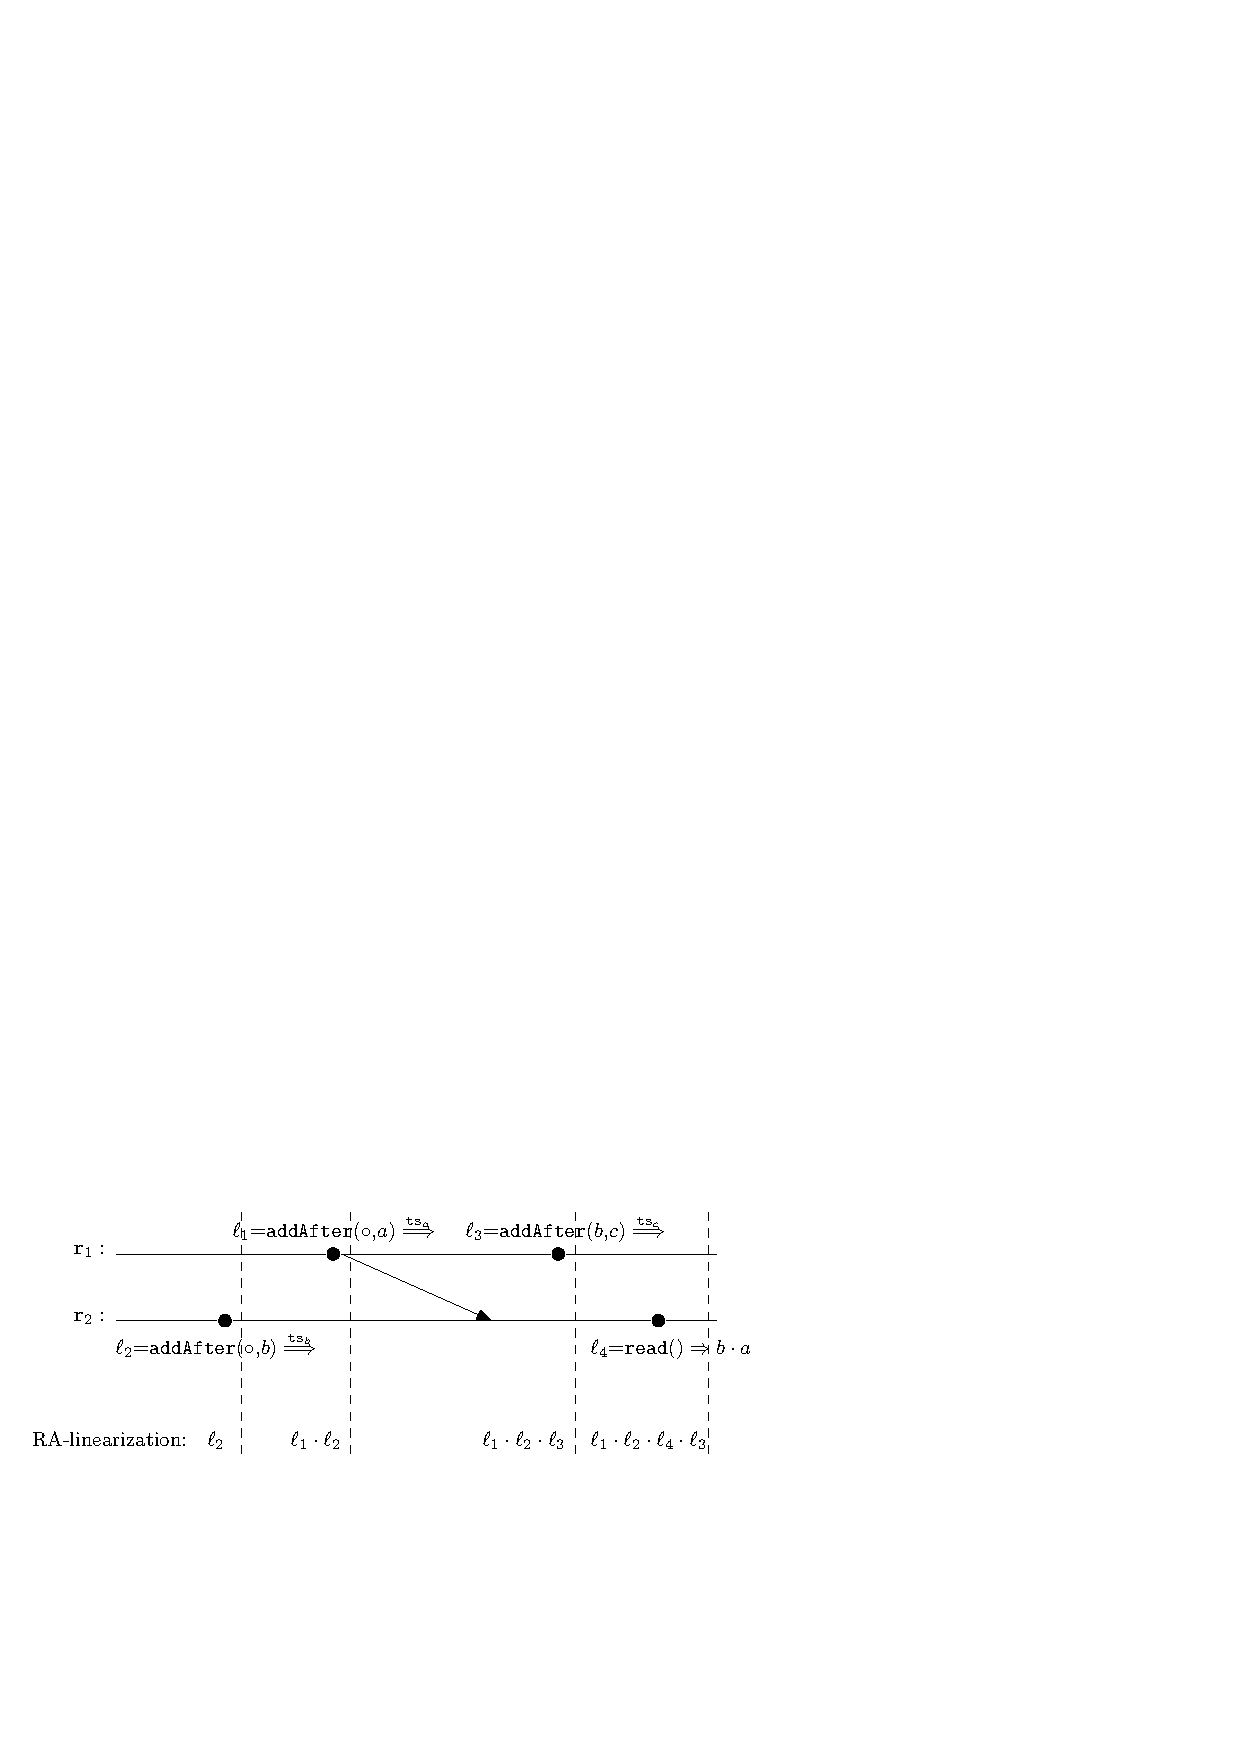
\includegraphics[width=0.7 \textwidth]{figures/RGAHisandLin.pdf}
%\vspace{-10pt}
  \caption{An execution of RGA and the corresponding execution-order and timestamp-order linearizations. We assume that $\ats_a<\ats_b<\ats_c$.}
  \label{fig:a history of RGA and its RA-linearization}
\end{figure}

CRDT objects such as RGA in Listing~\ref{lst:rga}, that use timestamps for conflict resolution, may not admit execution-order linearizations. 
For instance, \figureautorefname~\ref{fig:a history of RGA and its RA-linearization} shows an execution of RGA where two replicas $\arep_1$ and $\arep_2$ execute two ${\tt addAfter}$ invocations, and an ${\tt addAfter}$ invocation followed by a ${\tt read}$ invocation, respectively. An execution-order linearization which by definition, is consistent with the order in which the operations are applied at the origin replica, will order $\alabelshort[{\tt addAfter}]{\circ,b}$ before $\alabelshort[{\tt addAfter}]{\circ,a}$. The result of applying these two operations in this order in the specification $\specRGA$ (defined in Example~\ref{definition:sequential specification of rga}) is the list $a\cdot b$. However, as explained in \sectionautorefname~\ref{sec:rga-crdt-impl}, assuming that the timestamp $\ats_a$ associated to the element $a$ is smaller than the timestamp $\ats_b$ associated to $b$, the query ${\tt read}$ that sees these two operations will return the list $b\cdot a$, which is different than the one obtained by applying the same operations in the context of $\specRGA$ in linearization order. This shows that such a linearization is not a valid RA-linearization (w.r.t. $\specRGA$).
To prove that such objects are \crdtlinearizable{}, we consider another instantiation of the proof methodology described in \sectionautorefname~\ref{ssec:proof-methodology} where the linearization is additionally \emph{consistent with the order of timestamps} generated by the operations.
We describe this instantiation using the RGA as an example (showing that it is RA-linearizable w.r.t. $\specRGA$).

%\gpnote{I think this example is kinda complicated. Maybe add picture?}
The construction of the linearization ensures that the operations that generate a timestamp, i.e., the invocations of ${\tt addAfter}$, are ordered in the linearization according to their timestamps. For instance, if we consider the execution in \figureautorefname~\ref{fig:a history of RGA and its RA-linearization}, $\alabelshort[{\tt addAfter}]{\circ,a}$ will be ordered before $\alabelshort[{\tt addAfter}]{\circ,b}$ because $\ats_a$ is smaller than $\ats_b$ (even though they are executed in a different order at their origin replica). 
%More precisely, for any two operations $\alabelshort[{\tt addAfter}]{a,b}$ and $\alabelshort[{\tt addAfter}]{c,d}$ that generate two timestamps $\ats_{\tt b}$ and $\ats_{\tt d}$, respectively, the linearization should order $\alabelshort[{\tt addAfter}]{a,b}$ before $\alabelshort[{\tt addAfter}]{c,d}$ if $\ats_{\tt b}<\ats_{\tt d}$ and $\alabelshort[{\tt addAfter}]{c,d}$ before $\alabelshort[{\tt addAfter}]{a,b}$ if $\ats_{\tt d}<\ats_{\tt b}$. 
%
Moreover, to extend the notion of timestamp ordering to operations $\alabel$ that don't generate timestamps, i.e., invocations of ${\tt remove}$ and ${\tt read}$, we consider a ``virtual'' timestamp which is defined as the \emph{maximal} timestamp of any operation visible to $\alabel$ (or $\bot$ if no operation is visible to $\alabel$), and then require that the linearization is consistent with the order between both ``real''~\footnote{That is, timestamps generated by the operation itself.} and ''virtual'' timestamps. For instance, the {\tt read} operation in \figureautorefname~\ref{fig:a history of RGA and its RA-linearization} sees $\alabelshort[{\tt addAfter}]{\circ,a}$ and $\alabelshort[{\tt addAfter}]{\circ,b}$, therefore, its ``virtual'' timestamp is $\ats_b$. Then, a valid RA-linearization will order the {\tt read} operation before the other $\alabelshort[{\tt addAfter}]{b,c}$ operation, since the timestamp $\ats_c$ of the latter is bigger than the ``virtual'' timestamp $\ats_b$ of the {\tt read}. The operations that have the same timestamp~\footnote{Among operations that have the same timestamp $\ats$, there is exactly one operation generating $\ats$, the rest of the operations having $\ats$ as a ``virtual'' timestamp (i.e., they don't generate timestamps themselves and the maximal timestamp they see is $\ats$).} are ordered as they execute at the origin replica. For instance, the {\tt read} operation with timestamp $\ats_b$ is ordered after $\alabelshort[{\tt addAfter}]{\circ,b}$ that has the same timestamp $\ats_b$ since it executes later at the origin replica.


The annotations defining the linearization are included under the
\lstinline|atSource| labels of Listing~\ref{lst:rga}. The function {\tt insert}($\alinord$,$\alabel$,$\ats$) inserts the label $\alabel$ in the linearization $\alinord$ just after the last operation $\alabel'$ in $\alinord$ which has a timestamp (real or virtual) smaller than or equal to $\ats$. The annotations characterizing the effectors are quite straightforward in this case, since they are straightforward logical interpretations of the program statements.

The proof of $\mathsf{ReplicaStates}$ is quite similar to the case of OR-Set. Since the order between the timestamps generated by ${\tt addAfter}$ operations is consistent with the visibility relation (see \sectionautorefname~\ref{ssec:semantics}), it easily follows that the linearization order $\alinord$ is also consistent with the visibility relation. Then, as in the case of OR-Set, it remains to prove that any two effectors that correspond to two ``concurrent'' operations (not related by visibility) commute. This easily follows from the fact that the effectors apply set union which is obviously commutative. Also, note that by the causal delivery assumption and the preconditions of ${\tt addAfter}$ and ${\tt remove}$, it cannot happen that an $\alabelshort[{\tt addAfter}]{a,b}$ operation adding ${\tt b}$ after ${\tt a}$ is concurrent with an operation that adds ${\tt a}$ to the list, i.e., $\alabelshort[{\tt addAfter}]{c,a}$, for some ${\tt c}$, or that an $\alabelshort[{\tt addAfter}]{a,b}$ operation adding ${\tt b}$ is concurrent with an operation $\alabelshort[{\tt remove}]{b}$ that removes ${\tt b}$. This ensures that reordering concurrent effectors doesn't lead to ``invalid'' replica states where for instance, the timestamp tree ${\tt N}$ contains nodes which are not reachable from the root (which would happen if $\alabelshort[{\tt addAfter}]{a,b}$ is delivered before the operation $\alabelshort[{\tt addAfter}]{c,a}$ adding ${\tt a}$), or where the tombstone set ${\tt Tomb}$ contains elements which are not in the tree (which would happen if $\alabelshort[{\tt remove}]{b}$ is delivered before $\alabelshort[{\tt addAfter}]{a,b}$).

%{\color {red} CW: Each abstract state is in the form $\abstate = (a_1,flag_1) \cdot \ldots \cdot (a_n,flag_n)$.} 
Concerning the proof of $\mathsf{Refinement}$, we consider a refinement mapping $\refmap$ which relates a replica state ${\tt (N,Tomb)}$ with a specification state $(l,T)$ where the sequence of elements $l$ is given by the function ${\tt traverse}$ used in ${\tt read}$ operations by ignoring tombstones, i.e., $l={\tt traverse(N, \emptyset)}$, and $T={\tt Tomb}$. The fact that effectors of ${\tt remove}$ operations, and ${\tt read}$ queries are simulated by the corresponding operations of the specification is straightforward. Concerning effectors of $\alabellongind[{\tt addAfter}]{a,b}{}{\ats_b}{}$ operations, we show that they are simulated by the corresponding specification operation $\alabelshort[{\tt addAfter}]{a,b}$ only when the timestamp $\ats_{\tt b}$ is strictly greater than all the timestamps stored in the replica state where it applies. This is sufficient because, by $\mathsf{ReplicaStates}$, every replica state is obtained by applying effectors according to the linearization of their corresponding operations, and the linearization order is consistent with the timestamp order. Thus, let $({\tt N},{\tt Tomb})$ be a replica state such that $\ats_{\tt a} < \ats_{\tt b}$ for every $\ats_{\tt a}$ with $({\tt c},\ats_{\tt a},{\tt a})\in {\tt N}$ for some ${\tt c}$. The result of applying the effector $\effector$ corresponding to $\alabellongind[{\tt addAfter}]{a,b}{}{\ats_b}{}$ is to add ${\tt b}$ as a child of ${\tt a}$. Then, applying ${\tt traverse}$ on the new state will result in a sequence where ${\tt b}$ is placed just after ${\tt a}$ because it has the biggest timestamp among the children of ${\tt a}$ (and all the nodes in the tree ${\tt N}$). This corresponds exactly to the sequence obtained by applying the operation $\alabelshort[{\tt addAfter}]{a,b}$ in the context of the specification.

To prove that $\mathsf{\CRDTLinshort{}}$ is an inductive invariant, we use almost the same arguments as in the case of OR-Set. The two notable differences are that in this case, the specification doesn't admit any sequence of updates and also, that effectors of ${\tt addAfter}$ operations are simulated by the corresponding specification operations only under a certain condition related to timestamps. Concerning the first point, the specification requires that any $\alabelshort[{\tt addAfter}]{a,b}$ or $\alabelshort[{\tt remove}]{a}$ operation is preceded by an operation adding ${\tt a}$. However, since $\alinord$ is consistent with the visibility relation, and the preconditions of the RGA $\alabelshort[{\tt addAfter}]{a,b}$ and $\alabelshort[{\tt remove}]{a}$ operations ensure that an operation $\alabelshort[{\tt addAfter}]{c,a}$, for some ${\tt c}$, is visible when applying them at the origin replica, it follows that the projection of $\alinord$ on updates is admitted by the specification. Second, we have to show that the side-condition added to the simulation of ${\tt addAfter}$ effectors still guarantees that any sequence $\mathsf{effSeq}$ of effector applications consistent with the linearization order (considering only such sequences is possible because of the $\mathsf{ReplicaStates}$ invariant) can be simulated by the specification. This follows from the fact that the linearization order is consistent with the timestamps generated by operations, which implies that any ${\tt addAfter}$ effector adding an element ${\tt b}$ with timestamp $\ats_{\tt b}$ is ordered in $\mathsf{effSeq}$ after all ${\tt addAfter}$ effectors adding elements with timestamps smaller than $\ats_{\tt b}$.

Next, we present a formal definition of timestamp-order linearizations. For a history $\ahist=(\alabelset,\avisord)$, we define the timestamp $\tsof_\ahist(\alabel)$ of a label $\alabel$ in the context of the history $h$ to be $\tsof_\ahist(\alabel)=\tsof(\alabel)$ if $\tsof(\alabel)\neq\bot$ and $\tsof_\ahist(\alabel)=\mathsf{max}\, \{\tsof(\alabel'):(\alabel',\alabel)\in \avisord \}$, otherwise.

\begin{definition}
An object $\aobj$ which is \crdtlinearizable{} w.r.t. a specification $\Spec$ admits \emph{timestamp-order linearizations} if for every trace $\atrace\in\traces(\aobj)$ with $\hist{\atrace}=(\alabelset,\avisord)$, there exists an \crdtlinearization{} $(\alabelset,\alinord)$ of $\hist{\atrace}$ w.r.t. $\Spec$ such that $\alabel_1$ occurs before $\alabel_2$ in $\alinord$ iff $\tsof_\ahist(\alabel_1) < \tsof_\ahist(\alabel_2)$ or $\src{}{\alabel_1}$ occurs before $\src{}{\alabel_2}$ in $\atrace$, for every two labels $\alabel_1,\alabel_2\in\alabelset$.
\end{definition}

The following theorem shows the set of objects we have proved to be RA-linearizable and admit timestamp-order linearizations (also mentioned in \figureautorefname~\ref{fig:crdt-implementaton of this paper, their correctness, and their interface}). The specification of the LWW-register (short for Last Writer Wins Register) is standard, i.e., a read operation returns the last written value, while the specification of the LWW-Set is similar, the object storing a set of values instead of a single value like in the context of the LWW-register. The precise definitions of these specifications and the proofs can be found in the supplementary material.

\begin{theorem}\label{th:ts_order_objects}
LWW-Register, LWW-Set, and RGA are RA-linearizable and admit timestamp-order linearizations.
\end{theorem}

\fxwarning[nomargin, inline]{TODO SAY THAT RGA WITH ADDAT IS NOT RA-LINEARIZABLE}

%%% Local Variables:
%%% mode: latex
%%% TeX-master: "draft"
%%% End:


%!TEX root = draft.tex
%\newcommand{\seqPQ}{\mathsf{SeqPQ}}

\section{Compositionality of Distributed Linearizability}
\label{sec:compositionality of distributed linearizability}

\textblue{
This section should give three results of the form: if $o_1$ is linearizable w.r.t. $S_1$ and $o_2$ is linearizable w.r.t. $S_2$, and ???, then $o_1 \otimes o_2$ is linearizable w.r.t. $S_1\times S_2$ (the 2-object spec defined by interleavings). ??? may be an additional condition, while $\otimes$ is an "operator" for composing two CRDT implementations. Every result will have a different $\otimes$ operator.
\begin{itemize}
\item T0 + T0: ??? = $S_1$ and $S_2$ are $T0$-specs, and $\otimes$ is the trivial composition (the "unsynchronized" product)
\item T1 + T1: ??? = $S_1$ and $S_2$ are $T1$-specs, and $\otimes$ is the "shared counter" composition (the "unsynchronized" product with a restriction on the set of generated histories)
\item T0 + T1: ??? = $S_1$ is a $T_0$ spec, and $S_2$ is a $T1$-spec, and $\otimes$ is the "global causal delivery" composition (the "unsynchronized" product with a restriction on the set of generated histories)
\end{itemize}
Also, we should prove that composing two $T0$, resp., $T1$, specs results in a $T0$, resp., $T1$ spec, and composing a $T0$ with $T1$ results in a $T1$. With this, the extension to sets of objects is straightforward:  compose all $T0$ and independently, all $T1$, then compose the two resulting objects.}


\subsection{Definition of Compositionality}
\label{subsec:definition of compositionality}

The following is the definition of distributed linearizability for multi-object histories.

\begin{definition}[Distributed Linearizability for Multi-object Histories]
\label{definition:distributed linearizability for multi-object histories}
A multi-object history $h$ is \crdtlinearizable{}, if there exists a sequence $\mathit{lin}$, called linearization of $h$, such that

\begin{enumerate}[(i)]
\item The elements of $\mathit{lin}$ is generated from the operations of $h$: each operation $o = (m(a) \Rightarrow b,i,\mathit{obj})$ is transformed into $(m(a) \Rightarrow b,i,S)$ with $S$ set of identifiers of operations of visible to $o$ via $h.\mathit{vis}$.
\item $\mathit{lin}$ is consistent with $h. \mathit{vis}$.
\item For each object $\mathit{obj}$, $h \uparrow_{\mathit{obj}}$ is \crdtlinearizable{}, and $\mathit{lin} \uparrow_{ \mathit{obj} }$ is a \crdtlinearization{} of $h \uparrow_{\mathit{obj}}$.
\end{enumerate}

A set $H$ of multi-object histories are \crdtlinearizable{} w.r.t deterministic sequential specifications, if each of its history is.
\end{definition}

The following is the definition of compositional histories.

\begin{definition}[Compositionality]
\label{definition:compositionality}
A multi-object history $h$ is called compositional, if: $h \uparrow_{\mathit{obj}}$ is distributed linearizable for each object $\mathit{obj}$, if and only if, $h$ is distributed linearizable.
\end{definition}

It is easy to see that, a multi-object history $h$ being distributed linearizable implies that the projection of $h$ into each object is distributed linearizable. When proving compositionality, we only need to consider the opposite direction.




\subsection{T0-Linearizability and T1-Linearizability}
\label{subsec:t0-linearizability and t1-linearizability} 

To prove compositional 

T0-linearizability is a sub-class of distributed linearizability. 

\begin{definition}[t0-linearizability]
\label{definition:t0-ilnearizability}
A single-object history $h$ is t0-linearizable w.r.t a sequential specification $\mathit{spec}$, if each sequence $\mathit{lin}$ shown below is a linearization of $h$ w.r.t $\mathit{spec}$:

\begin{itemize}
\setlength{\itemsep}{0.5pt}
\item[-] Each element $(\ell,i,\mathit{vis}^{-1}(i))$ of $\mathit{lin}$ is generated from an operation $(\ell,i,\_,\mathit{ts})$ of $h$.

\item[-] $\mathit{lin}$ is consistent with $\mathit{vis}$.
\end{itemize}
\end{definition}

To prove t0-linearizability, we introduce the notion of t0-specifications. A specification $\mathit{spec}$ is called t0-specification, if given a history $h$ that is distributed linearizable w.r.t $\mathit{spec}$, then any sequence that is consistent with visibility relation is a linearization of $h$.

The following lemma shows some sequential specifications are t0-specifications. Its proof can be found in Appendix \ref{subsec:appendix proofs of Lemma several t0-specifications}. Based on this lemma and our proofs in Section \ref{sec:proving distributed linearizability}, we can see that or-set is t0-linearizable w.r.t $\mathit{OR}$-$\mathit{set}_s$, and counter is t0-linearizable w.r.t $\mathit{counter}_s$.

\begin{restatable}{lemma}{SeveralTZeroSpecifications}
\label{lemma:several t0-specifications}
$\mathit{OR}$-$\mathit{set}_s$, $\mathit{set}_s$ and $\mathit{counter}_s$ are t0-specifications.
\end{restatable}



Given a history $h$, a sequence $\mathit{lin}$ is called a strict time-stamp order candidate of $h$, if for each elements $o_1,o_2$ of $\mathit{lin}$, if the time-stamp of $o_1$ in $h$ is less than that of $o_2$, then, $o_1$ is before $o_2$ in $\mathit{lin}$. T1-linearizability is a sub-class of distributed linearizability.

\begin{definition}[t1-linearizability]
\label{definition:t1-ilnearizability}
A single-object history $h$ is t1-linearizable w.r.t a sequential specification $\mathit{spec}$, if each strict time-stamp order candidiate $\mathit{lin}$ is a linearization of $h$.
\end{definition}

To prove t1-linearizability, we introduce the notion of t1-specifications. A specification $\mathit{spec}$ is called t1-specification, if given a history $h$ that is distributed linearizable w.r.t $\mathit{spec}$, and has a strict time-stamp order candidate as linearization, then any strict time-stamp order candidate is a linearization of $h$.

The following lemma shows some sequential specifications are t1-specifications. Its proof can be found in Appendix \ref{subsec:appendix proofs of Lemma several t1-specifications}. Based on this lemma and our proofs in Section \ref{sec:proving distributed linearizability}, we can see that RGA is t1-linearizable w.r.t $\mathit{list}_s^{\mathit{af}}$, and LWW-register is t1-linearizable w.r.t $\mathit{reg}_s$.

\begin{restatable}{lemma}{SeveralTOneSpecifications}
\label{lemma:several t1-specifications}
$\mathit{list}_s^{\mathit{af}}$ and $\mathit{reg}_s$ are t1-specifications.
\end{restatable}


\begin{table}
  \centering
  \begin{tabular}[t]{l|l}
    T0 & $\mathit{OR}$-$\mathit{set}_s$, $\mathit{set}_s$, $\mathit{counter}_s$,  \\
    T1 & $\mathit{list}_s^{\mathit{af}}$, $\mathit{reg}_s$,
  \end{tabular}
\end{table}




\subsection{Composing Several t0-Specifications}
\label{lemma:several t0-specifications can be composed}

The following lemma states that a history of several objects of t0 specifications is compositional. Its proof can be found in Appendix \ref{subsec:appendix proofs of lemma several t0-specifications can be composed}.

\begin{restatable}{lemma}{composingTZero}
\label{lemma:several t0-specifications can be composed}
Given a multi-object history $h$, if each of its object uses a t0-specification, then, $h$ is compositional.
\end{restatable}




\subsection{Composing Several t0-Specifications with One T1-specification}
\label{lemma:composing several t0-specification with one t1-specification}

Composing several t0-specifications with one t1-specification does not hold in general. \figurename~\ref{fig:a failed example of composing a multi-value register with a last-write-win register} is a history $h$ that is a failed example of composing a multi-value register with a last-write-win register, where the operations of LWW register are boxed. Here we assume that $\mathit{ts}_1<\mathit{ts}_2$. Since multi-value register is t0-specification and LWW register is t1-specification, we can see that the projection of $h$ into operations of multi-value register is distributed linearization and the only possible linearization is $\mathit{write}(a) \cdot \mathit{write}(b)$, and the projection of $h$ into operations of LWW register is distributed linearization and the only possible linearization is $\mathit{write}(c) \cdot \mathit{write}(d)$. However, $h$ is not distributed linearizable, since there is a a cycle.

\begin{figure}[t]
  \centering
  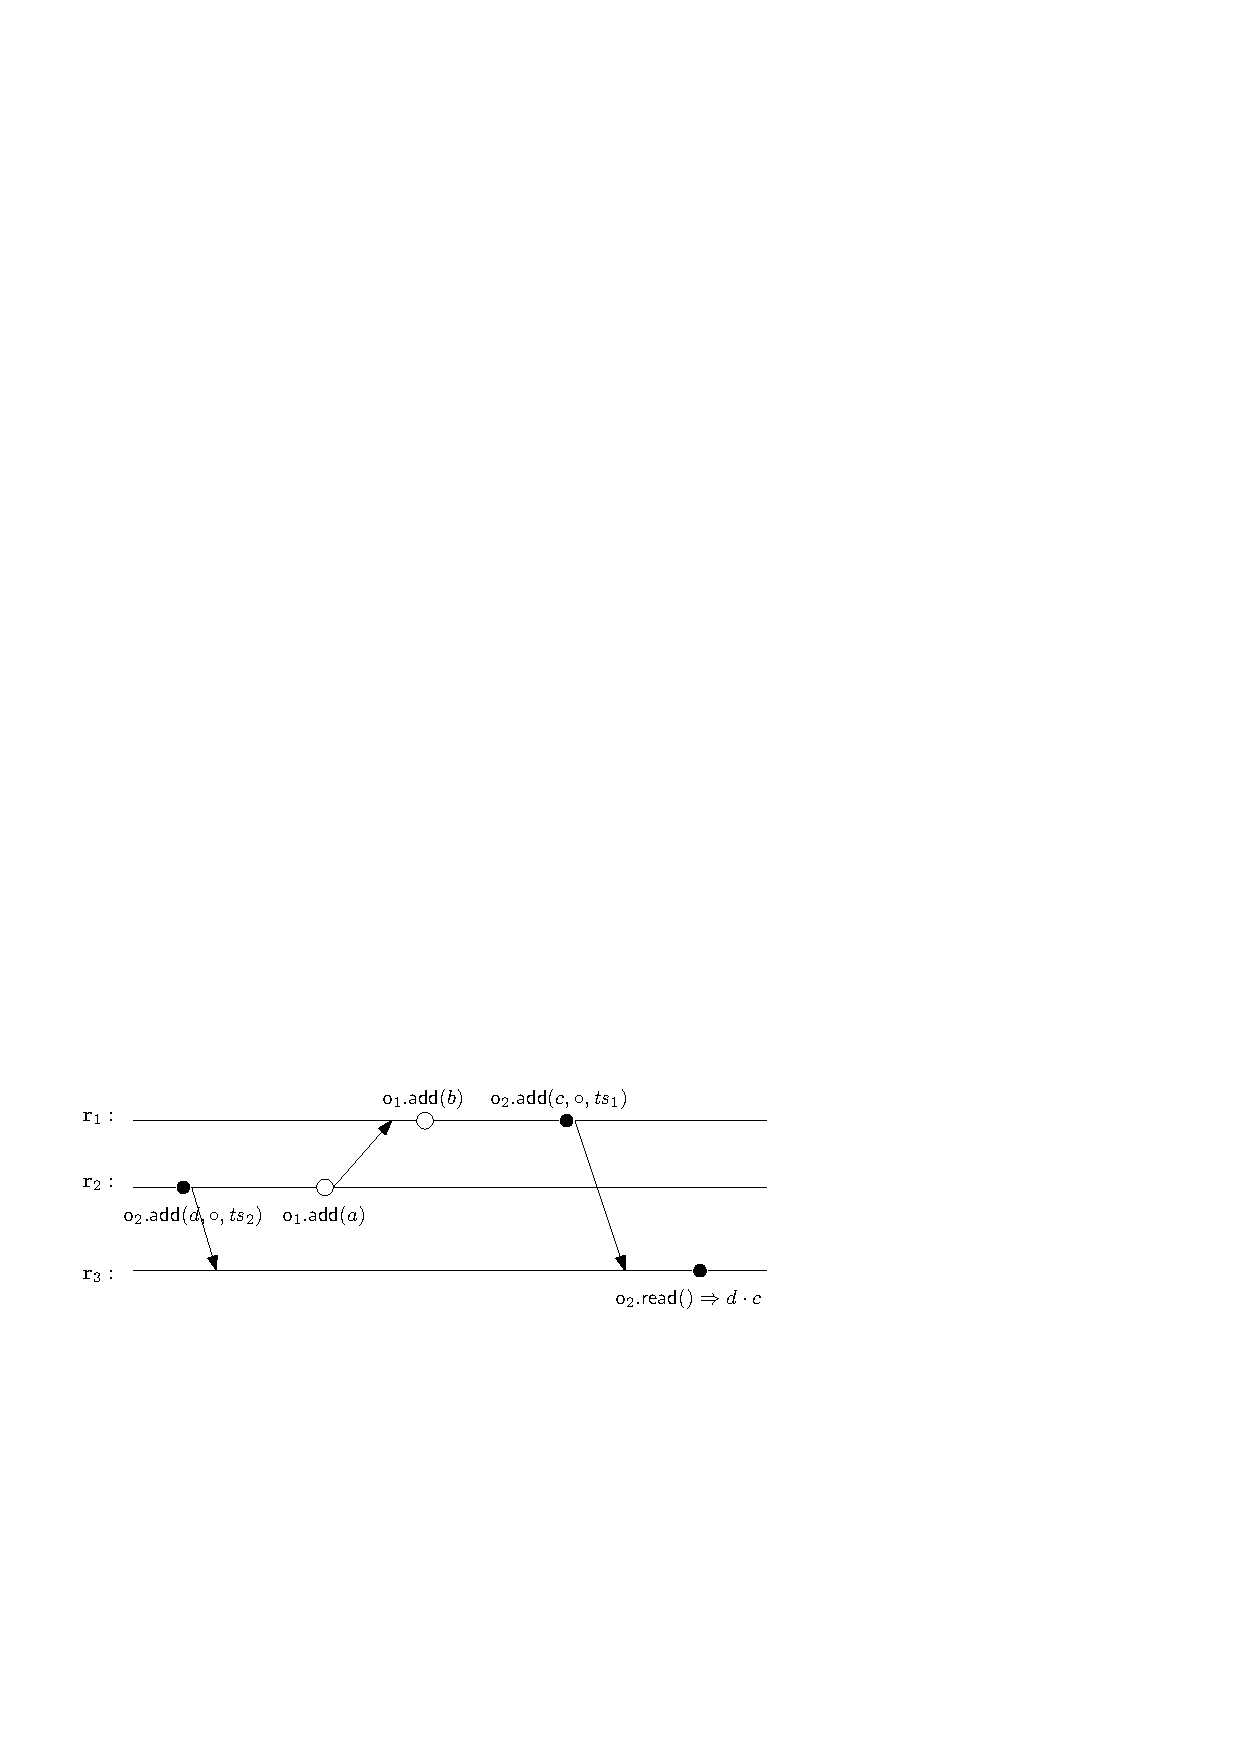
\includegraphics[width=0.6 \textwidth]{figures/MVReg-LWWReg-Nocd.pdf}
\vspace{-10pt}
  \caption{A failed example of composing a multi-value register with a last-write-win register (boxed operations), where $\mathit{ts}_1 < \mathit{ts}_2$.}
  \label{fig:a failed example of composing a multi-value register with a last-write-win register}
\end{figure}

The following lemma states that for a multi-object history, if its object use several t0-specifications and one t1-specification, and its visibility relation is transitive, then, $h$ is compositional. Its proof can be found in Appendix \ref{subsec:appendix proofs of lemma several t0-specifications and one t1-specification can be composed}.

\begin{restatable}{lemma}{composingTZeroAndOneTOne}
\label{lemma:several t0-specifications and one t1-specification can be composed}
Given a multi-object $h$, if its object use several t0-specifications and one t1-specification, and its visibility relation is transitive, then, $h$ is compositional.
\end{restatable}




\subsection{Composing Several t0-Specifications with Several T1-specification}
\label{lemma:composing several t0-specification with several t1-specification}

Composing several t0-specifications with several t1-specification does not hold in general. \figurename~\ref{fig:a failed example of composing two last-write-win registers} is a history $h$ that is a failed example of composing two last-write-win registers, where the operations of one LWW register are boxed, and the operations of the other LWW registers are not boxed. Here we assume that $\mathit{ts}_1 < \mathit{ts}_2 < \mathit{ts}_3$, and $\mathit{ts}'_1 < \mathit{ts}'_2$. Since LWW register is t1-specification, we can see that the projection of $h$ into operations of one LWW register is distributed linearization and the only possible linearization is $\mathit{write}(a,\mathit{ts}'_1) \cdot \mathit{write}(b,\mathit{ts}'_2)$, and the projection of $h$ into operations of the other LWW register is distributed linearization and the only possible linearization is $\mathit{write}(c,\mathit{ts}_1) \cdot \mathit{write}(d,\mathit{ts}_2) \cdot \mathit{write}(e,\mathit{ts}_3)$. However, $h$ is not distributed linearizable, since there is a a cycle.

\begin{figure}[t]
  \centering
  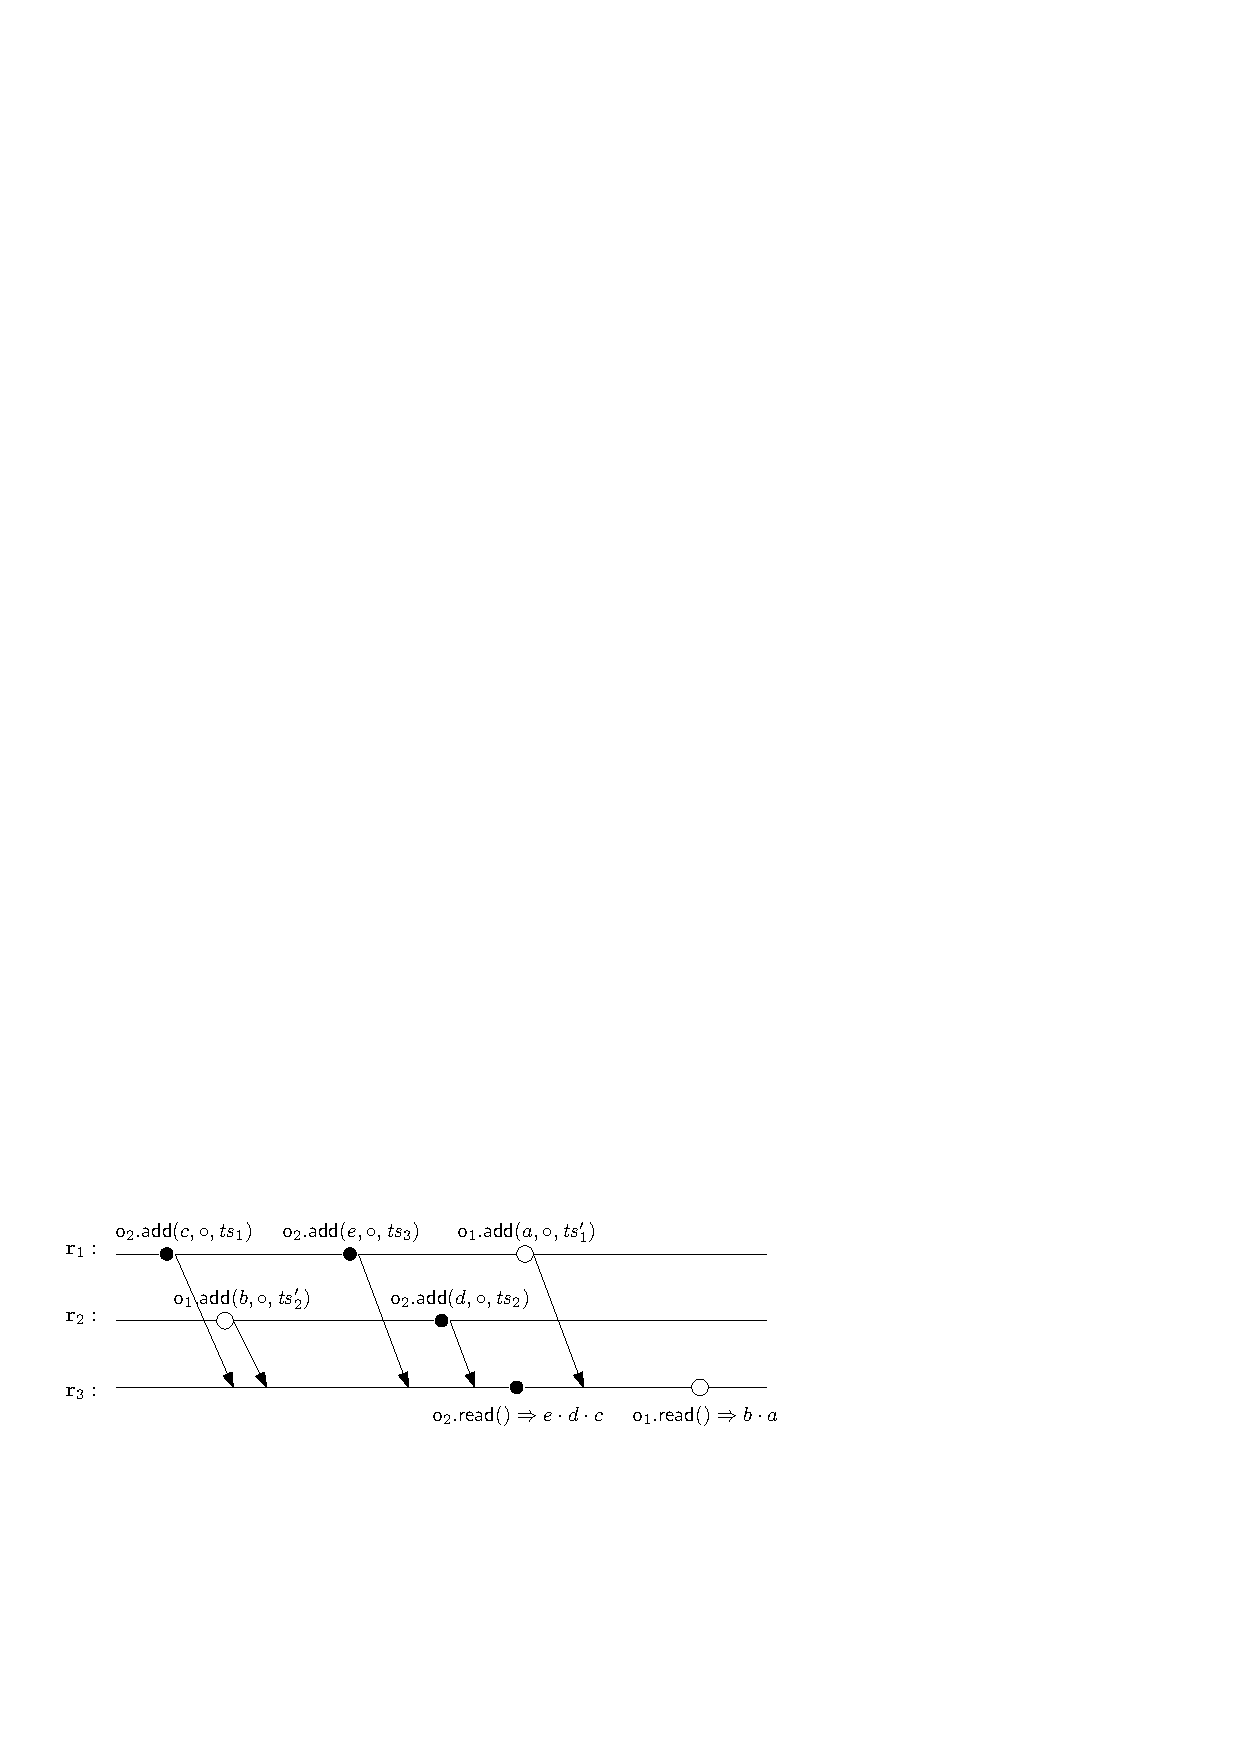
\includegraphics[width=0.7 \textwidth]{figures/LWWReg-LWWReg-NoSTS.pdf}
\vspace{-10pt}
  \caption{A failed example of composing two last-write-win registers (one object is boxed, the other is not), where $\mathit{ts}_1 < \mathit{ts}_2 < \mathit{ts}_3$, and $\mathit{ts}'_1 < \mathit{ts}'_2$.}
  \label{fig:a failed example of composing two last-write-win registers}
\end{figure}


A history $h$ satisfies causal-time-stamp, if: Given operation $o_1,\ldots,o_{\mathit{2k+2}}$ of $h$ that are of objects of t1-specification, if

\begin{itemize}
\setlength{\itemsep}{0.5pt}
\item[-] $(o_2,o_3)$ are of a same object, $\ldots$, $(o_{\mathit{2k}},o_{\mathit{2k+1}})$ are of a same object, $(o_{\mathit{2k+2}},o_1)$ are of a same object,

\item[-] $\mathit{ts}(o_2) < \mathit{ts}(o_2)$, $\ldots$, and $\mathit{ts}(o_{\mathit{2k}}) < \mathit{ts}(o_{\mathit{2k+1}})$,

\item[-] $(o_1,o_2), \ldots, (o_{\mathit{ek+1}},o_{\mathit{2k+2}}) \in \mathit{vis}$.
\end{itemize}

Then, we have $\mathit{ts}(o_1) < \mathit{ts}(o_{\mathit{2k+1}})$.

The following lemma states that for a multi-object history, if its object use several t0-specifications and several t1-specification, and it satisfies causal-time-stamp and its visibility relation is transitive, then, $h$ is compositional. Its proof can be found in Appendix \ref{subsec:appendix proofs of lemma several t0-specifications and several t1-specification can be composed}.

\begin{restatable}{lemma}{composingTZeroAndTOne}
\label{lemma:several t0-specifications and several t1-specification can be composed}
Given a multi-object $h$, if its object use several t0-specifications and several t1-specification, and it satisfies causal-time-stamp and its visibility relation is transitive, then, $h$ is compositional.
\end{restatable}






\subsection{Modified CRDT Implementation}
\label{subsec:modified CRDT implementation}

To ensure composing, we modify t1-algorithms as follows: The system supplies a method called $\mathit{updateGlobalTS}$, which supplies a time-stamp that is updated along the global system. When a method needs to generate new time-stamp, it calls this method to generate new time-stamp, and such process will also update the global time-stamp of this replica. When a method sends a message, the message should contain the current global time-stamp value. When a replica receives a message, it also use the global time-stamp value in message to update its own global time-stamp value. Moreover, the global time-stamp satisfies causal-time-stamp property.

The RGA algorithm after modification is as follows: Here a message contains the current global time-stamp value, and a replica update global time-stamp value is not explicitly written in code. Instead, such processes will be make explicit when constructing the operational semantics.

\begin{lstlisting}[caption={Pseudo-code of the Modified RGA}, captionpos=b,label={lst:modifier rga}]
  payload Ti-Tree N, Set Tomb
  initial N = @|$\emptyset$|@, Tomb = @|$\emptyset$|@

  addAfter(a,b) :
    atSource :
      precondition : b = @|$\circ$|@ or (b != @|$\circ$|@ and (b,_,_) @|$\in$|@ N and b @|$\not\in$|@ Tomb)
      let ts@|$_{\mathtt{a}}$|@ = updateGlobalTS()
      let ts@|$_{\mathtt{b}}$|@ = (b == @|$\circ$|@)?(0,r@|$_{0}$|@):(timestamp of b in N)
    downStream(a, ts@|$_{\mathtt{a}}$|@, ts@|$_{\mathtt{b}}$|@) :
      precondition: b = @|$\circ$|@ or (b != @|$\circ$|@ and (b, ts@|$_{\mathtt{b}}$|@,_) @|$\in$|@ N)
      N = N ts@|$\cup$|@ {(a, ts@|$_{\mathtt{a}}$|@, ts@|$_{\mathtt{b}}$|@)}

  remove(a) :
    atSource :
      precondition : a != @|$\emptyset$|@ and (a,_,_) @|$\in$|@ N and a @|$\notin$|@ Tomb
    downStream(a) :
      precondition : a != @|$\emptyset$|@ and (a,_,_) @|$\in$|@ N
      Tomb = Tomb @|$\cup$|@ {a}

  read() :
    return traverse(N, Tomb)
\end{lstlisting}


The following lemma states that the modified RGA is also t1-linearizable w.r.t $\mathit{list}_s^{\mathit{af}}$, and the modified LWW-register is t1-linearizable w.r.t $\mathit{reg}_s$. Its proof can be found in Appendix \ref{a}.

\begin{restatable}{lemma}{ModifiedRGAandLWWRegStillTOne}
\label{lemma:modified RGA and LWW-register is still t1-linearizable}
$\mathit{list}_s^{\mathit{af}}$ and $\mathit{reg}_s$ are t1-specifications.
\end{restatable}

Lamport's time-stamp is one way to implement global time-stamp, as stated by the following lemma. Its proof can be found in Appendix \ref{a}.

\begin{restatable}{lemma}{LamportTSasGlobalTS}
\label{lemma:lamport time-stamp as global time-stamp}
Lamport's time-stamp satisfies causal-time-stamp.
\end{restatable}








\subsection{Semantics of Multi Objects}
\label{subsec:semantics of multi objects}

When there is multiple objects, we say $(o_1,o_2) \in \mathit{vis}$, if either $(o_1,o_2) \in \mathit{ro}$, or $o_1$ is delivered to the replica of $o_2$ before $o_2$ happens. We consider CTDT implementation of t1-specifications use the time-stamp of Lamport's time-stamp: Each time-stamp is a tuple $(c,r)$ of a counter value $c \in \mathbb{N}$ and a replica identifier $r \in \mathbb{R}$; $(c_1,r_1) < (c_2,r_2)$, if $c_1 < c_2 \vee (c_1 = c_2 \wedge r_1 < r_2)$. To ensure compositionality of multiple objects, the following conditions needs to be satisfied:

\begin{itemize}
\setlength{\itemsep}{0.5pt}
\item[-] Cross-object-causal-delivery (COCD): We extend the notion of causal-delivery into multiple objects. Given two update operations $o_1$ and $o_2$, and assume $o_1$ is visible to $o_2$. Then, for each replica, once it receives $o_2$, it must be the case that $o_1$ has been previously received.

\item[-] Shared-time-stamp (STS): the objects of t1-specifications shares a counter $\mathit{sCtr}$. Each message carries a value of $\mathit{sCtr}$, and when generating new message, the value of $\mathit{sCtr}$ is also considered.
\end{itemize}



Based on shared-time-stamp,



Formally, given a set $\mathit{Objs}$ of objects, its semantics is defined as $\llbracket \mathit{Objs} \rrbracket_{\mathit{op}} = (\mathit{Config},\mathit{config}_0,\Sigma',\rightarrow)$ as in \figurename~\ref{fig:the semantics of multiple operation-based CRDT object}.


\begin{figure}[ht]
$\mathit{RState} = \mathit{Objs} \times \mathbb{R} \rightarrow \Sigma$

$\mathit{TState} = \mathbb{MID} \times \mathbb{MSG} \times \mathbb{R} \times \mathit{Objs}$

$\mathit{MsgHB} \subseteq \mathbb{MID} \times \mathbb{MID}$

$\mathit{MsgDel} \subseteq \mathbb{MID} \times \mathbb{R}$

$\mathit{Config} = \mathit{RState} \times \mathit{TState} \times \mathit{MsgHB} \times \mathit{MsgDel}$, $\mathit{config}_0 \in \mathit{Config}$.

$\Sigma' = \mathit{do}(\mathit{Objs} \times \mathbb{M} \times \mathbb{D} \times \mathbb{D} \times \mathbb{R} \times \mathbb{MID}) \cup \mathit{do}(\mathit{Objs} \times \mathbb{M} \times \mathbb{D} \times \mathbb{D} \times \mathbb{R}) \cup \mathit{receive}(\mathit{Objs} \times \mathbb{MID} \times \mathbb{R})$

\begin{itemize}
\setlength{\itemsep}{0.5pt}
\item[] $\begin{array}{l c}
   \bigfrac{
   \begin{array}{c}
     R(x,r) = \sigma, (x,r).\mathit{do}(\sigma,m,a) = (\sigma',b,\mathit{msg}), \mathit{msg} \neq \emptyset, \mathit{unique}(\mathit{mid}), \\
     S_1 = \{ (\mathit{mid}',\mathit{mid}) \vert (\mathit{mid'},r) \in \mathit{MsgDel} \}, S_2 = \{ (\mathit{mid}',\mathit{mid}) \vert \mathit{mid}' \in T, \mathit{mid}' \ is \ of \ replica \ r \}
   \end{array}}
     {(R,T,\mathit{msgHB},\mathit{MsgDel}) {\xrightarrow{\mathit{do}(x,m,a,b,r,\mathit{mid})}} (R[(x,r):\sigma'], T \cup \{ (\mathit{mid},\mathit{msg},r,x) \}, (\mathit{MsgHB} \cup S_1 \cup S_2)^*,\mathit{MsgDel})}
\end{array}$

\item[] $\begin{array}{l c}
   \bigfrac{
   \begin{array}{c}
     R(x,r) = \sigma, (x,r).\mathit{do}(\sigma,m,a) = (\sigma',b,\emptyset)
   \end{array}}
     {(R,T,\mathit{msgHB},\mathit{MsgDel}) {\xrightarrow{\mathit{do}(x,m,a,b,r)}} (R[(x,r):\sigma'], T \cup \{ (\mathit{mid},\mathit{msg},r) \}, \mathit{MsgHB},\mathit{MsgDel})}
\end{array}$

\item[-] $\begin{array}{l c}
   \bigfrac{
   \begin{array}{c}
      R(x,r) = \sigma, (x,r).\mathit{receive}(\sigma,\mathit{msg}) = \sigma', (\mathit{mid},\mathit{msg},r',x) \in T, r \neq r', \\
      (\mathit{mid},r) \notin \mathit{MsgDel}, \mathit{mid} \ is \ minimal \ w.r.t \ \mathit{MsgHB} \ among \ \{ \mathit{mid}' \vert (\mathit{mid}',r) \notin \mathit{MsgDel} \}
   \end{array}}
     {(R,T,\mathit{msgHB},\mathit{MsgDel}) {\xrightarrow{\mathit{receive}(x,\mathit{mid},r)}} (R,T,\mathit{MsgHB},\mathit{MsgDel} \cup \{ (\mathit{mid},r) \} )}
\end{array}$
\end{itemize}
\caption{The definition of semantics of $\llbracket \mathit{Objs} \rrbracket_{\mathit{op}}$}
\label{fig:the semantics of multiple operation-based CRDT object}
\end{figure}




$R$ is now a function from object and replica identifier to local state. Message and action also record its object. $\mathit{MsgHB}$ and $\mathit{MsgDel}$ now record the relation between messages of multiple objects. In each transition rule of \figurename~\ref{fig:the semantics of multiple operation-based CRDT object}, we deal with each object according to its CRDT implementations. Similarly, a sequence $l$ of actions is an execution of $\llbracket \mathit{Objs} \rrbracket_{\mathit{op}} = (\mathit{Config},\mathit{config}_0,\Sigma',\rightarrow)$, if there exists $(R,T,\mathit{MsgHB},\mathit{MsgDel}) \in \mathit{Config}$, such that $\mathit{config}_0 {\xrightarrow{ l }} (R,T,\mathit{MsgHB},\mathit{MsgDel})$. The semantics of $\mathit{Objs}$ is defined as the set of executions of $\llbracket \mathit{Objs} \rrbracket_{\mathit{op}}$.





A configuration $(R,T,\mathit{MsgHB},\mathit{MsgDel})$ is a snapshot of distributed system. $R$ gives the local state of each replica, and $T$ gives the set of messages that has been generated. Let $\mathbb{MID}$ be the set of message identifiers of message content. A message is a tuple $(\mathit{mid},\mathit{msg},r)$, where $\mathit{mid} \in \mathbb{MID}$ is the identifier, $\mathit{msg} \in \mathbb{MSG}$ is the message content, and $r$ is the original replica of message. $\mathit{MsgHB}$ is used to record the happen-before relation between messages: two messages $(\mathit{mid}_1,\mathit{mid}_2) \in \mathit{MsgHB}$ represents that the operation of $\mathit{mid}_1$ happens before the operation of $\mathit{mid}_2$. $\mathit{MsgDel}$ is used to record the message delivery relation between messages: $(\mathit{mid},r) \in \mathit{MsgDel}$ represents that message $\mathit{mid}_1$ has already been delivered to replica $r$. $\mathit{MsgHB}$ and $\mathit{MsgDel}$ are used to ensure message delivery requirements. $\mathit{config}_0$ is the initial configuration, which maps each replica into the initial local state, has no message, and with a empty happen-before relation and a empty message delivery relation.


Each element of $\Sigma'$ is called an action. $\rightarrow \in \mathit{Config} \times \Sigma' \times \mathit{Config}$ is the transition relation and describes a single step of distributed systems. The first rule in \figurename~\ref{fig:the semantics of a operation-based CRDT object} describes replica $r$ performs a update operation $m(a) \Rightarrow b$ and generates a message with message content $\mathit{msg}$. Here $\mathit{unique}$ is a function that ensures $\mathit{mid}$ be a fresh message identifier. We insert message identifier $\mathit{mid}$ into the happen-before relation and keeps the happen-before relation be transitive. The second rule describes replica $r$ performs a query operation $m(a) \Rightarrow b$ and thus does not generate message. Since no message is generated, the $\mathit{MsgHB}$ and $\mathit{MsgDel}$ tuples remain the same. The third rule describes delivery of a message to a replica $r$ other than its origin replica $r'$. By $(\mathit{mid},r) \notin \mathit{MsgDel}$, we ensure that $\mathit{mid}$ has not been previously delivered to replica $r$, and thus, each message be delivered to each replica at most once. By $\mathit{mid}$ being minimal w.r.t $\mathit{MsgHB}$ among $\{ \mathit{mid}' \vert (\mathit{mid}',r) \notin \mathit{MsgDel} \}$, we always choose a minimal element w.r.t $\mathit{MsgHB}$ among operations not been delivered to a replica, and thus, ensures causal-delivery.



\subsection{Proving in Multi-Objects Semantics}
\label{subsec:proving in multi-object semantics}


The formation of CRDT in this semantics is changed as follows,

The CRDT proved distributed linearizable are still distributed linearizable in this new semantics.


%%% Local Variables:
%%% mode: latex
%%% TeX-master: "draft"
%%% End:


%\section{CRDT-Linearizable Implementations}
%\label{sec:crdt-lin-imp}

%\gpn{Proofs of CRDT-Linearizable implementations}

%\begin{itemize}
%\item Counters
%  \begin{itemize}
%  \item Grow-Only Counter
%  \item PN-Counter
%  \end{itemize}
%\item Registers:
%  \begin{itemize}
%  \item LWW
%  \item MVR
%  \end{itemize}
%\item Sets:
%  \begin{itemize}
%  \item LAW (OR-Set)
%  \item Grow-Only Set
%  \end{itemize}
%\item Text-Editing (Graphs/Lists)
%  \begin{itemize}
%  \item RGA (addRight)
%  \item WOOT
%  \end{itemize}
%\end{itemize}

% \section{Meta-properties of CRDT-Linearizability}
% \label{sec:meta-prop-lincrdt}

% % \subsection{Compositionality}
% % \label{sec:compositionality}

% % \gpn{Here we explain the compositionality result a la Herlihy Wing}

% % \begin{itemize}
% % \item What are the conditions for compositionality (deterministic
% %   specs?, conflict?)
% %   \begin{itemize}
% %   \item Can we share the same timestamp for different data structures.
% %   \item Coherent conflict resolution.
% %   \end{itemize}
% % \item Should we change the implementations to change the
% %   conflict-resolution.
% % \end{itemize}

% \subsection{Abstraction}
% \label{sec:abstraction}

% \gpn{Here we explain refinement}
% \begin{itemize}
% \item What is the power of the client? Messages, other calls to CRDTs?
% \item Observational refinement?
% \item Completeness?
% \end{itemize}

%% Bibliography
\bibliography{biblio}

\newpage

\appendix

\section{\crdtimp{}}
\label{sec:crdt implementation}



\subsection{Multi-Value Register Implementation}
\label{subsec:multi-value register implementation}

\cite{ShapiroPBZ11} shows how to obtain a state-based \crdtimp{} from a operation-based \crdtimp{}, and we draw it in Listing~\ref{lst:operation-based emulation of state-based object}. To do an operation $f(a)$, we compute the state-based update and perform merge method in downstream. Here the precondition of downstream is empty because merge is always enabled.


\begin{minipage}[t]{1.0\linewidth}
\begin{lstlisting}[frame=top,caption={operation-based emulation of state-based object},
captionpos=b,label={lst:operation-based emulation of state-based object}]
  payload S ( the state-based payload )
  initial initial payload of S

  update method f(a)
    atSource :
      precondition : precondition of f(a)
      let s = atSource of f(a) in state-based
    downStream(s) :
      S = merge(S,s)
\end{lstlisting}
\end{minipage}

\cite{ShapiroPBZ11} gives a state-based multi-value register implementation. As discussed above, we give its operation-based version in Listing~\ref{lst:operation-based multi-value register}. Here $myRep()$ is a function that returns current replica identifier, and $reps()$ is a function that returns the number of replicas in distributed system. This implementation assumes that the number of replicas are fixed. A payload $S$ is a set of $(a,V)$ pairs, where $a$ is a value and $V$ is a vector called version vector. %Annotation1 is an annotation for the current payload, and annotation2 is an annotation for downstream of $write(a)$.
Given vector clock $V$ and $V'$, we say that $V > V'$, if for each replica $\arep$, we have $V[\arep] > V'[\arep]$. Annotation1 is an annotation for downstream of $write(a)$.


\begin{minipage}[t]{1.0\linewidth}
\begin{lstlisting}[frame=top,caption={Pseudo-code of operation-based multi-value register},
captionpos=b,label={lst:operation-based multi-value register}]
  payload Set S
  initial S = @|$\emptyset$|@
  initial seq = @|$\epsilon$|@

  write(a) :
    atSource :
      let g = myRep()
      let @|$\mathcal{V}$|@ = @|$\{ V \vert \exists x, (x,V) \in S \}$|@
      let @|$V'$|@ = @|$[ max_{V \in \mathcal{V}} V[j]]_{j \neq g}$|@
      let @|$V'[g]$|@ = @|$max_{V \in \mathcal{V}} V[g]$|@ + 1
      //@ let seq@|$'$|@ = seq@|$\,\cdot\,\alabellongind[readIds]{}{S}{}\,\cdot\,\alabelshort[write]{a,V',S}$|@
    downStream(a, V@|$'$|@) :
      let A = @|$\{ (a_1,V_1) \in S \vert \neg V' > V_1 \}$|@
      let B = @|$\{ (a,V') \}$|@, if @|$\forall (a_1,V_1) \in S, \neg V_1 > V'$|@. Otherwise, let B = @|$\emptyset$|@
      S = A @|$\cup$|@ B
      //@ Annotation1 : @|$\forall \arep, V'[\arep]$|@ = @|$\vert \{ \alabel = \alabellongind[write]{\_,\_}{\bot}{*}, \alabel$|@ happens on replica @|$\arep,  (\alabel,\alabelshort[write]{a,V'}) \in \avisord \vee \alabel = \alabelshort[write]{a,V'} \} \vert$|@

  read() :
    let @|$S_1$|@  = {a : @|$\exists$|@ V. (a,V) @|$\in$|@ S}
    //@ let seq@|$'$|@ = seq@|$\,\cdot\,\alabellongind[read]{}{S_1}{}$|@
    return @|$S_1$|@
\end{lstlisting}
\end{minipage}

%//@ Annotation1 : S =  @|$\{ (a,V) \vert \exists \alabel = \alabellongind[write]{a,V}{\bot}{*}, \alabel$|@ is maximal w.r.t @|$\avisord$|@ among write operations applied in current replica @|$\}$|@





\subsection{The WOOT Algorithm}
\label{subsec:the woot algorithm}

The WOOT algorithm of \ref{a} is given in Listing~\ref{lst:woot algorithm}. Note that here $integrateIns$ is a recursive method used by $addBetween$ method.

In local of each replica, WOOT algorithm stores the list as a sequence of W-characters. A W-character $w$ is a five-tuple $<id,v,flag,id_p,id_n>$, where $id$ is the identifier of $w$; $v$ is the value of $w$; $flag \in \{ \mathit{true},\mathit{false} \}$ is the flag of $w$ and indicates whether $w$ is ``visible'' in list; $id_p$ and $id_n$ is the identifier of the previous and next W-character of $w$, respectively. The previous and the next W-characters of $w$ are the W-characters between which $w$ has been inserted on its generation state. Given $w = (id,v,flag,id_p,id_n)$, let $C_P(w) = id_p$ and $C_N(w) = id_n$ denote the previous and next W-character of $w$, respectively. A identifier $id$ of W-character is a tuple $(ctr,\arep)$, where $ctr \in \mathbb{N}$.

A W-string is an ordered sequence of W-characters $w_b \cdot w_1 \cdot \ldots \cdot w_n \cdot w_e$, where $w_b$ and $w_e$ are special W-characters that mark the beginning and the ending of the sequence. The values of $w_b$ and $w_e$ are $\circ_b$ and $\circ_e$, respectively. We define the following function for a W-string $str$:

\begin{itemize}
\setlength{\itemsep}{0.5pt}
\item[-] $\vert str \vert$ returns the length of $str$,

\item[-] $str[p]$ returns the W-character at position $p$ in $str$. Her we assume that the first element of $str$ is at position 0.

\item[-] $pos(str,w)$ returns the position of W-character $w$ in $S$.

\item[-] $insert(str,w,p)$ inserts W-character $w$ into $str$ at position $p$.

\item[-] $subseq(str,w_1,w_2)$ returns the part of $str$ between the W-characters $w_1$ and $w_2$ (excluding $w_1$ and $w_2$).

\item[-] $contains(str,a)$ returns true if there exists a W-character in $str$ with value $a$.

\item[-] $values(str)$ returns the sequence of visible (with $\mathit{true}$ flag) values of $str$.

\item[-] $getWchar(str,a)$ returns the W-character with value $a$ in $str$.

\item[-] $changeFlag(str,pos,f)$ changes the flag of $str[pos]$ into $f$.
\end{itemize}

%Note that only $values(str)$ distinguish whether a W-character is with flag $\mathit{true}$ or with flag $\mathit{false}$.

A total order $<_{id}$ is given for identifiers of W-characters for conflict resolution. Given two identifiers $(ctr_1,\arep_1)$ and $(ctr_2,\arep_2)$, we have $(ctr_1,\arep_1) <{id} (ctr_2,\arep_2)$, if $\arep_1 < \arep_2 \vee (\arep_1 = \arep_2 \wedge ctr_1 < ctr_2)$. Given a sequence $str$ and two elements $a,b$ of $str$, we write $a <_{str} b$ to indicate that $pos(str,a) < pos(str,b)$.

\begin{minipage}[t]{1.0\linewidth}
\begin{lstlisting}[frame=top,caption={Pseudo-code of WOOT algorithm},
captionpos=b,label={lst:woot algorithm}]
  payload int @|$H_s$|@, W-string @|$string_s$|@
  initial @|$H_s$|@ = 0, @|$string_s$|@ = @|$\epsilon$|@
  initial seq = @|$\epsilon$|@

  addBetween(a,b,c) :
    atSource :
      precondition :  @|$contains(string_s,b) \wedge contains(string_s,c) \wedge pos(string_s,c) - pos(string_s,b) = 1\wedge \neg contains(string_s,a)$|@
      let g = myRep()
      let @|$c_p$|@ = @|$getWchar(string_s,b)$|@
      let @|$c_n$|@ = @|$getWchar(string_s,c)$|@
      @|$H_s$|@ = @|$H_s$|@ + 1
      //@ let seq@|$'$|@ = seq@|$\,\cdot\,\alabellongind[addBetween]{a,b,c}{}{}$|@
    downStream((w,@|$c_p$|@,@|$c_n$|@)) : with @|$w = ((H_s,g),a,\mathit{true},c_p.id,c_n.id)$|@
      integrateIns(@|$w,c_p,c_n$|@)

  remove(a) :
    atSource :
      precondition : @|$contains(string_s,a)$|@
      let w = @|$getWchar(string_s,a)$|@
      //@ let seq@|$'$|@ = seq@|$\,\cdot\,\alabellongind[remove]{a}{}{}$|@
    downStream(w) :
      let p = @|$pos(string_s,w)$|@
      @|$changeFlag(string_s,p,\mathit{false})$|@

  read() :
    let s = @|$values(string_s)$|@
    //@ let seq@|$'$|@ = seq@|$\,\cdot\,\alabellongind[read]{}{s}{}$|@
    return s

  integrateIns(@|$c,c_p,c_n$|@)
    let @|$S$|@ = @|$string_s$|@
    let @|$S'$|@ = @|$subseq(S,c_p,c_n)$|@
    if @|$S' = \epsilon$|@
      then  @|$insert(S,c,pos(S,c_n))$|@
    else
      Let L = @|$c_p \cdot d_0 \cdot \ldots \cdot d_m \cdot c_n$|@, where @|$d_0, \ldots, d_m$|@ are the W-characters in @|$S'$|@
        such that for each @|$d_i$|@, @|$C_P(d_i) <_S c_p$|@ and @|$c_n <_S C_N(d_i)$|@ 
      Let i = 1 
      while (@|$i < \vert L \vert -1 \wedge L[i] <_{id} c$|@) do
        i = i+1 
      integrateIns(@|$c,L[i-1],L[i]$|@)  
\end{lstlisting}
\end{minipage}

The payload of each replica is a integer value $H_s$ used to generate identifier, and a W-string $string_s$.

To do $addBetween(a,b,c)$, we first ensure that $b$ and $c$ are adjacent in $string_s$ and $a$ is not in $string_s$. Then, we generate a W-character $w$ for value $a$, and calls method $integrateIns(w,c_p,c_n)$ to put $w$ between $c_p$ and $c_n$, which are the W-characters of $b$ and $c$ in $string_s$, respectively. 

$integrateIns(c,c_p,c_n)$ is a recursive method and works as follows: If there are no W-character between $c_p$ and $c_n$ (for example, in the current replica), then $w$ is put after $c_p$. Else, WOOT select a set $L$ of W-characters, such that each W-character of $L$ has a ranger ``wider than the range between $c_p$ and $c_n$''. The W-characters in $L$ are the W-characters that needs to be considered when the range is between $c_p$ and $c_n$. It can be proved that W-characters in $L$ are sorted by the $<_{id}$ order. Then, we choose the position of $c$ to be between $L[i-1]$ and $L[i]$. We can see that the range between $L[i-1]$ and $L[i]$ is strictly shorter than the range between $c_p$ and $c_n$. Since there may be W-characters in the range between $L[i-1]$ and $L[i]$ in $string_s$, we make a recursive call to $integrateIns(c,L[i-1],L[i])$ to compute the position of $c$ in the range between $L[i-1]$ and $L[i]$. 

To do $remove(a)$, we just set the flag of W-character of $a$ in $string_s$ to be $\mathit{false}$. To do $read()$, we return $values(string_s)$. 







\section{Sequential Specifications}
\label{sec:sequential specifications}

%In this section we give several sequential specifications.


\subsection{The Sequential Specification of Counter}
\label{subsec:the sequential specification of counter}

The sequential specification $\mathit{counter}_s$ of counter is so that $\abstates = \mathbb{Z}$, that is the state will be an integer, and the transitions are given as follows:
\begin{itemize}
\setlength{\itemsep}{0.5pt}
\item[-] $k \xrightarrow{\alabellong[\mathsf{inc}]{}{}} k+1$
\item[-] $k \xrightarrow{\alabellong[\mathsf{dec}]{}{}} k-1$
\item[-] $k \xrightarrow{\alabellong[\mathsf{read}]{}{k}} k$
\end{itemize}

Here $inc$ increase the counter by $1$, $dec$ decrease the counter by $1$, and $read$ returns the value of the counter.



\subsection{The Sequential Specification of Multi-Value Register}
\label{subsec:the sequential specification of multi-value register}

The query-update rewriting of multi-value register is as follows: $\gamma( \alabellong[\mathsf{write}]{a}{} ) = ( \alabellong[\mathsf{readIds}]{}{S}, \alabellong[\mathsf{write}]{a,id,S}{})$.


Each abstract state $\abstate$ is a set of tuples $(a,id)$, where $a$ is a data and $id$ is a identifier. The sequential specification $\mathit{mvreg}_s$ of multi-value register is given with the transitions as follows:

\begin{itemize}
\setlength{\itemsep}{0.5pt}
\item[-] $\abstate \xrightarrow{\alabellong[\mathsf{readIds}]{}{\abstate}} \abstate$

\item[-] $\big(\abstate\ |\ (a,id) \notin \abstate \big) \xrightarrow{ \alabellong[\mathsf{write}]{a,id,S}{} }  \abstate \setminus S \cup \{ (a,id) \}$

\item[-] $\abstate \xrightarrow{\alabellong[\mathsf{read}]{}{ \{ a \vert \exists id, (a,id) \in \abstate \} }} \abstate$
\end{itemize}

Here $readIds$ returns the abstract state, $\alabellong[\mathsf{write}]{a,id,S}{}$ removes $S$ from the abstract state and puts $\{ (a,id) \}$ into the abstract state, and $read$ returns the value of multi-value register.



\subsection{The Sequential Specification of List with Add-Between Interface}
\label{subsec:the sequential specification of list with add-between interface}

Each abstract state $\abstate$ is a sequence of tuples $(a,flag)$, where $a$ is a data and $flag \in \{ \mathit{true},\mathit{false} \}$ is flag. $(a,\mathit{true})$ means that $a$ is in the list, while $(a,\mathit{false})$ means that $a$ has once been added into the list and then removed. The sequential specification $\mathit{listBet}_s$ of list with add-between interface is given with the transitions as follows:

\begin{itemize}
\setlength{\itemsep}{0.5pt}
\item[-] $\big(\abstate\ |\ \abstate = (a_1,flag_1)\cdot \ldots \cdot (a_n,flag_n) \wedge 1 \leq i \leq k < j \leq n \wedge (a,\_) \notin \abstate \big) \xrightarrow{ \alabellong[\mathsf{addBetween}]{a,a_i,a_j}{} } (a_1,flag_1)\cdot \ldots (a_k,flag_k) \cdot (a,\mathit{true}) \cdot (a_{k+1},flag_{k+1}) \cdot \ldots \cdot (a_n,flag_n)$

\item[-] $\big(\abstate\ |\ \abstate = (a_1,flag_1)\cdot \ldots \cdot (a_n,flag_n) \wedge 1 \leq k \leq n \big) \xrightarrow{ \alabellong[\mathsf{remove}]{a_k}{} } (a_1,flag_1)\cdot \ldots (a_k,\mathit{false}) \cdot \ldots \cdot (a_n,flag_n)$

\item[-] $(a_1,flag_1)\cdot \ldots \cdot (a_n,flag_n) \xrightarrow{\alabellong[\mathsf{read}]{}{ s }} (a_1,flag_1)\cdot \ldots \cdot (a_n,flag_n)$, here $s$ is the projection of $a_1 \cdot \ldots \cdot a_n$ into $\{ a \vert a$ is with flag $\mathit{true} \}$
\end{itemize}

$\alabellong[\mathsf{addBetween}]{a,a_i,a_j}{}$ puts $(a,\mathit{true})$ into a random position between $(a_i,\_)$ and $(a_j,\_)$, and we assume that each value is put into list at most once. $\alabellong[\mathsf{remove}]{a_k}{}$ removes $a_k$ from the list by setting its flag into $\mathit{false}$. $read$ returns the content of list. value of multi-value register.

Assume that the initial value of list is $(\circ_b,\mathit{true}) \cdot (\circ_e,\mathit{true})$, and $\circ_b$ and $\circ_e$ are never removed. When the context is clear, in $\mathit{read}$ operation, we will omit $\circ_b$ and $\circ_2$ in return value.










\section{Proofs of \crdtimp}
\label{sec:appendix proofs of crdt implementations}



\subsection{Proof of Operation-Based Multi-Value Register}
\label{subsec:proof of operation-based multi-value register}

Given two sequences $l_1,l_2$  such that $l_2$ is a permutation of $l_1$, let $\mathit{diff}(l_1,l_2) = \{ (a,b) \vert$ the order of $a$ and $b$ in $l_1$ is different from that of $l_2 \}$. Given a sequence $l$ and two elements $a$ and $b$ of $l$, let $\mathit{swap}(l,a,b)$ be a sequence obtained from $l$ by swapping $a$ and $b$. The following lemma states that, given two specification sequences $(\alabelset_1, \aseqord_1)$ and $(\alabelset, \aseqord_2)$ that are generated from a same history and both consistent with visibility relation, we can obtain $\aseqord_2$ from $\aseqord_1$ by several time of swapping adjacent pair of concurrent operations.

\begin{lemma}
\label{lemma:given two sequence consistent with visibility order, one can be obtained from the other}
Given a history $(\alabelset,\avisord)$ and two two specification sequences $(\alabelset_1, \aseqord_1)$ and $(\alabelset, \aseqord_2)$ that are both consistent with $\avisord$. If $\aseqord_1 \neq \aseqord_2$, then we can obtain $\aseqord_2$ from $\aseqord_1$ by several time of swapping adjacent pair of concurrent operations.
\end{lemma}

\begin {proof}

First, we need to prove that, if $\mathit{diff}(\aseqord_1,\aseqord_2) \neq \emptyset$, then, there exists $(\alabel_1,\alabel_2) \in \mathit{diff}(\aseqord_1,\aseqord_2)$, such that $l_1$ and $l_2$ are concurrent, and $l_1$ and $l_2$ are adjacent in $\aseqord_1$.

We prove this by contradiction. Assume $\mathit{diff}(\aseqord_1,\aseqord_2) \neq \emptyset$, and for each $(\alabel_1,\alabel_2) \in \mathit{diff}(\aseqord_1,\aseqord_2)$, we have that either $\alabel_1$ and $\alabel_2$ are not concurrent, or $\alabel_1$ and $\alabel_2$ are not adjacent in $\aseqord_1$.

Since $\mathit{diff}(\aseqord_1,\aseqord_2) \neq \emptyset$, let $(\alabel,\alabel')$ be a element of $\mathit{diff}(\aseqord_1,\aseqord_2)$, and the distance of $\alabel$ and $\alabel'$ is minimal in $\{$ the distance between $\alabel_1$ and $\alabel_2 \vert (\alabel_1,\alabel_2) \in \mathit{diff}(\aseqord_1,\aseqord_2) \}$. Let us prove that $\alabel$ and $\alabel'$ are adjacent by contradiction: If there exists $\alabel''$ between $\alabel$ and $\alabel'$. Assume that in $\aseqord_1$, $\alabel$ is before $\alabel''$, and $\alabel''$ is before $\alabel'$. By assumption, the order between $\alabel$ and $\alabel''$, and between $\alabel''$ and $\alabel'$ is the same in $\aseqord_1$ and in $\aseqord_2$. This implies that $\alabel$ is still before $\alabel'$ in $\aseqord_2$, which contradicts the fact that $(\alabel,\alabel') \in \mathit{diff}(\aseqord_1,\aseqord_2)$.

Since $\alabel$ and $\alabel'$ are adjacent and $(\alabel,\alabel') \in \mathit{diff}(\aseqord_1,\aseqord_2)$, by assumption we know that $\alabel$ and $\alabel'$ are not concurrent. Or we can say, $(\alabel,\alabel') \in \avisord \vee (\alabel',\alabel) \in \avisord$. This contradicts that both $\aseqord_1$ and $\aseqord_2$ are consistent with visibility relation. This completes the proof of the first part.

Since $\aseqord_1 \neq \aseqord_2$, we have $\mathit{diff}(\aseqord_1,\aseqord_2) \neq \emptyset$, and then, as discussed above, there exists $(\alabel,\alabel') \in \mathit{diff}(\aseqord_1,\aseqord_2)$, such that $\alabel$ and $\alabel'$ are concurrent, and $\alabel$ and $\alabel'$ are adjacent in $\aseqord_1$. Let $\aseqord_3 = \mathit{swap}(\aseqord_1,\alabel,\alabel')$. It is easy to see that $\mathit{diff}(\aseqord_1,\aseqord_2) > \mathit{diff}(\aseqord_3,\aseqord_2)$. Therefore, by several times of above process, we finally obtain $\aseqord_2$ from $\aseqord_1$ by swapping pairs of operations. This completes the proof of this lemma. $\qed$
\end {proof}


Then, let us prove that the operation-based multi-value register implementation is \crdtlinearizable{} w.r.t $\mathit{mvreg}_s$.

\begin{lemma}
\label{lemma:multi-value register is correct}
The operation-based multi-value register implementation is \crdtlinearizable{} w.r.t $\mathit{mvreg}_s$
\end{lemma}


\begin {proof}

Let us give two facts:

\begin{itemize}
\setlength{\itemsep}{0.5pt}
\item[-] $fact1$: Let $(a_1,V_1)$ and $(a_2,V_2)$ be the downstream for $\alabel_1$ and $\alabel_2$, respectively, and assume that $(\alabel_1,\alabel_2) \in \avisord$. Then, $V_1 < V_2$.
\item[-] $fact2$: Let $(a_1,V_1)$ and $(a_2,V_2)$ be the downstream for $\alabel_1$ and $\alabel_2$, respectively, and assume that $\alabel_1$ and $\alabel_2$ are concurrent. Then, $\neg (V_1 < V_2 \vee V_2 < V_1)$.

%\item[-] $fact3$: Let $S$ be the payload of a replica. Then, $S$ =  $\{ (a,V) \vert \exists \alabel = \alabellongind[write]{a,V}{\bot}{*}, \alabel$ is maximal w.r.t $\avisord$ among write operations applied in current replica $\}$.
\end{itemize}


\noindent Proof of $fact1$: Assume $\alabel_1$ happens on replica $\arep$. By the {\textred{causal delivery}} assumption, we know that for each replica $\arep' \neq \arep$, $\alabel_2$ see more or equal number of operations happens on replica $\arep'$ than that of $\alabel_1$, and $\alabel_2$ see more number of operations happens on replica $\arep$ than that of $\alabel_1$. By Annotation1, we know that $\forall \arep' \neq \arep$, $V_1[\arep'] \geq V_2[\arep']$, and $V_1[\arep] > V_2[\arep]$. Therefore, $V_1 < V_2$.

\noindent Proof of $fact2$: Let us prove that $\neg (V_1 < V_2 \vee V_2 < V_1)$ by contradiction. It is obvious that $\alabel_1$ and $\alabel_2$ happens on different replicas. Assume that $V_1 < V_2$, and assume that $\alabel_1$ happens on replica $\arep_1$. Since $V_1 < V_2$, we know that $V_1[\arep_1] \leq V_2[\arep_1]$. By the {\textred{causal delivery}} assumption and Annotation1, this means $(\alabel_1,\alabel_2) \in \avisord$, contradicts the assumption that $\alabel_1$ and $\alabel_2$ are concurrent. Similarly, we can see that $\neg (V_2 < V_1)$. Therefore, $\neg (V_1 < V_2 \vee V_2 < V_1)$.

Let us propose Annotation2, which is an annotation of payload and obviously holds in the initial global configuration.

\begin{itemize}
\setlength{\itemsep}{0.5pt}
\item[-] Annotation2: Let $S$ be the payload of a replica. Then, $S$ =  $\{ (a,V) \vert \exists \alabel = \alabellongind[write]{a,V}{\bot}{*}, \alabel$ is maximal w.r.t $\avisord$ among write operations applied in current replica $\}$.
\end{itemize}

Our proof of the lemma proceed as follows:

\begin{itemize}
\setlength{\itemsep}{0.5pt}
\item[-] We need to prove that $\mathsf{ReplicaStates}$ is an inductive invariant.

Since every operation is appended to the linearization when it executes {\tt atSource} it clearly follows, the linearization order is consistent with visibility order. Then, by the {\textred{causal delivery}} assumption, the order in which downstreams are applied at a given replica is also consistent with the visibility order. Let $\aseqord_1$ be the projection of linearization order into labels applied in a replica $\arep$, and $\aseqord_2$ be the order of labels applied in replica $\arep$. By Lemma \ref{lemma:given two sequence consistent with visibility order, one can be obtained from the other}, $\aseqord_2$ can be obtained from $\aseqord_1$ by several time of swapping adjacent pair of concurrent operations.

Let us prove that applying downstream of such pair of operations commute, and we only need to consider the case of two concurrent $write$ labels. Let $(a_1,V_1)$ and $(a_2,V_2)$ be the downstream of labels $\alabellongind[write]{a_1,V_1}{\bot}{*}$ and $\alabellongind[write]{a_2,V_2}{\bot}{*}$, respectively. Given a payload $S$, assume we obtained $S'$ from $S$ by applying $(a_1,V_1)$ and then applying $(a_2,V_2)$, and assume we obtained $S''$ from $S$ by applying $(a_2,V_2)$ and then applying $(a_1,V_1)$. In the process of obtaining $S'$ or $S''$ from $S$, we add $(a_1,V_1)$ and $(a_2,V_2)$ into $S$ and remove the following tuple $(a_3,V_3) \in S \cup \{(a_1,V_1),(a_2,V_2)\}$: either $V_3 < V_1$, or $V_3 < V_2$, or $(a_3,V_3) = (a_1,V_1) \wedge V_1 < V_2$, or $(a_3,V_3) = (a_2,V_2) \wedge V_2 < V_1$. Since we already know that $\alabellongind[write]{a_1,V_1}{\bot}{*}$ and $\alabellongind[write]{a_2,V_2}{\bot}{*}$ are concurrent, by  $fact_2$, we know that $\neg (V_1 < V_2 \vee V_2 < V_1)$. Therefore, $S' = S''$.



\item[-] Let we prove that the Annotation1 and Annotation2 is an inductive invariant.

We prove by induction on executions. Obvious they hold in $\aglobalstate_0$. Assume they hold along the execution $\aglobalstate_0 \xrightarrow{}^* \aglobalstate$ and there is a new transition $\aglobalstate \xrightarrow{} \aglobalstate'$. We need to prove that they still hold in $\aglobalstate'$. We only need to consider $write$ action or downstream:

    \begin{itemize}
    \setlength{\itemsep}{0.5pt}
    \item[-] For case of a $\alabellongind[write]{a,V'}{\bot}{*}$ action of replica $\arep$: Let $S$ and $S'$ be the payload of replica $\arep$ of $\aglobalstate$ and $\aglobalstate'$, respectively. Obviously $S' = \{ (a,V') \}$.

        Since $\alabellongind[write]{a,V'}{\bot}{*}$ is larger than any labels in $S$ w.r.t the visibility relation, Annotation2 still holds in $\aglobalstate'$.

        By Annotation2 we know what labels are contained in $S$, by Annotation1 we know the content of these labels. By the {\textred{causal delivery}} assumption we know that if a label $\alabel$ is visible to a label $\alabel'$ of $S$, then $\alabel$ must be already applied in replica $\arep$. let $\mathcal{V} = \{ V \vert (\_,V) \in S \}$ be the set of vector clocks of $S$. Therefore, for each replica $\arep' \neq \arep$, $max_{V \in \mathcal{V}} V[\arep']$ is the number of operations happen on replica $\arep'$ and has been applied in replica $\arep$ during $\aglobalstate_0 \xrightarrow{}^* \aglobalstate$, and $max_{V \in \mathcal{V}} V[\arep]$ is the number of operations happen on replica $\arep$ during $\aglobalstate_0 \xrightarrow{}^* \aglobalstate$. We can see that, for each replica $\arep' \neq \arep$, $V'[\arep'] = max_{V \in \mathcal{V}} V[\arep']$, and $V'[\arep] = max_{V \in \mathcal{V}} V[\arep] +1$. Therefore, Annotation1 still holds in $\aglobalstate'$.

    \item[-] For case of applying downstream $(a,V')$: We only need to consider Annotation2. Let $S$ and $S'$ be the payload of replica $\arep$ of $\aglobalstate$ and $\aglobalstate'$, respectively.

        By the {\textred{causal delivery}} assumption, if $\alabellongind[write]{a,V'}{\bot}{*}$ is visible to a operation $\alabel$, then $\alabel$ does not applied in $\aglobalstate'$ yet. By Annotation2, $fact1$ and $fact2$, we know that, $\forall (b,V) \in S$, we have $\neg(V > V')$. Therefore, we have $S' = S \setminus \{ (b,V) \vert (b,V) \in S \wedge V < V' \} \cup \{ (a,V') \}$. By $fact1$ and $fact2$, each element in $\{ (b,V) \vert (b,V) \in S \wedge V < V' \}$ is visible to $\alabellongind[write]{a,V'}{\bot}{*}$, and they are not in $S'$. Therefore, Annotation2 still holds in $\aglobalstate'$.
    \end{itemize}

\item[-] Let us prove that $\mathsf{Refinement}$ holds. We consider a refinement mapping $\refmap$ defined as the identity.

    \begin{itemize}
    \setlength{\itemsep}{0.5pt}
    \item[-] For $(a,V')$ and $write(a,V',S_1)$:

    Assume we obtain payload $S'$ from $S$ by doing downstream of $(a,V')$, in sequential specification have $\abstate \xrightarrow{write(a,V',S_1)} \abstate'$, and $\refmap(S) = \abstate$, or we can say, $S = \abstate$. We need to prove that $S' = \abstate'$.

    By the {\textred{causal delivery}} assumption, if $(\alabellongind[write]{a,V'}{\bot}{*},\alabel) \in \avisord$, then the downstream of $\alabel$ is not applied yet in the replica of $S$. By Annotation2, $fact1$ and $fact2$, we can see that, $\forall (b,V) \in S$, $\neg(V > V')$. Therefore, according to the implementaiton, we can see that $S' = S \setminus S_2 \cup \{ (a,V') \}$, where $S_2 = \{ (b,V) \vert (b,V) \in S \wedge V < V' \}$.

    According to Annotation2, we can see that, $S_1 = \{ (b,V) \vert \exists \alabel = \alabellongind[write]{b,V}{\bot}{*}, (b,V)$ is the downstream of $l, l$ is maximal among $write$ operations visible to $\alabellongind[write]{a,V'}{\bot}{*} \}$. We can see that $\abstate' = \abstate \setminus S_1 \cup \{ (a,V') \}$.

    Let us prove $S' = \abstate'$ by contradiction.

        \begin{itemize}
        \setlength{\itemsep}{0.5pt}
        \item[-] If there exists item $(c,V'')$ in $\abstate'$ but not in $S'$: we can see that $(c,V'') \in S$, $(c,V'') \notin S_1$, and $(c,V'') \in S_2$.

        Since $(c,V'') \notin S_1$, we know that there exists a $write$ operation $\alabel$, such that $(\alabellongind[write]{c,V''}{\bot}{*},\alabel),(\alabel,\alabellongind[write]{a,V'}{\bot}{*}) \in \avisord$. Since $(c,V'') \in S$, we can see that the downstream $\alabel$ is not applied yet in the replica of $S$, while in $S'$, the downstream of $\alabellongind[write]{a,V'}{\bot}{*}$ is applied. This violates the {\textred{causal delivery}} assumption.

        \item[-] If there exists item $(c,V'')$ in $S'$ but not in $S\abstate'$: we can see that $(c,V'') \in S$, $(c,V'') \notin S_2$, and $(c,V'') \in S_1$.

        Since $(c,V'') \notin S_2$, we know that $\neg(V'' < V)$. Since $(c,V'') \in S_1$, we know that $(\alabellongind[write]{c,V''}{\bot}{*},\alabellongind[write]{a,V'}{\bot}{*}) \in \avisord$. This contradicts $fact1$ and $fact2$.
        \end{itemize}

    Therefore, we know that $S' = \abstate'$, and the case of $(a,V')$ and $write(a,V',S_1)$ holds.

    \item[-] When the query-update $\alabelshort[write]{a}$ executes {\tt atSource} on a state $S$, then the query $\alabellong[readIds]{}{R}{}$ (introduced by the query-update rewriting) should be enabled in state $\refmap(S)=\abstate$, which clearly holds because the computation of $R$ in {\tt atSource} returns $S$, and the result of $\alabelshort[readIds]{}$ in the specification state $\abstate = S$ also returns $S$.

    \item[-] Applying the query $\alabelshort[read]{}$ on the payload $S$ should result in the same return value as applying the same query in the context of the specification on the same state $\abstate = \refmap(S)$, which again holds trivially.
    \end{itemize}

\item[-] Finally, we describe the proof of the fact that $\mathsf{\CRDTLinshort{}}$ is an inductive invariant. As already mentioned, appending operations to the linearization when they execute {\tt atSource} clearly implies that $\aseqord$ is consistent with the visibility. Next, the projection of $\aseqord$ on the updates is obviously admitted by the specification (the updates are always enabled from the point of view of the specification).
We also have to argue that for each query $\alabel_{\mathsf{qr}}\in\{\alabellongind[readIds]{}{R}{},\alabellongind[read]{}{A}{}\}$, the sequence $\aseqord'\cdot \alabel_{\mathsf{qr}}$ where $\aseqord'$ is the projection of $\aseqord$ on the set of updates
visible to $\alabel_{\mathsf{qr}}$ is admitted by the specification. First, by $\mathsf{ReplicaStates}$, the state $\sigma$ of the replica where $\alabel_{\mathsf{qr}}$ is applied is obtained by applying the downstreams of the operations visible to $\alabel_{\mathsf{qr}}$ in the linearization order. Then, by $\mathsf{Refinement}$, every downstream is simulated by the corresponding operation in the context of the specification. This implies that $\refmap(\sigma_0)\xRightarrow{\aseqord'}\refmap(\sigma)$, where $\sigma_0$ is the initial replica state. The query $\alabel_{\mathsf{qr}}$ is also simulated by the same operation in the context of the specification, which implies that $\refmap(\sigma)\xRightarrow{\alabel_{\mathsf{qr}}}\refmap(\sigma)$. These two facts imply that $\refmap(\sigma_0)\xRightarrow{\aseqord'\cdot \alabel_{\mathsf{qr}}}\refmap(\sigma)$ which means that $\aseqord'\cdot \alabel_{\mathsf{qr}}$ is admitted by the specification.
\end{itemize}

This completes the proof of this lemma. $\qed$
\end {proof}
















\section{\crdtlin{} with Non-Deterministic Sequential Specifications and Its Proof}
\label{sec:appendix RA-linearizability with non-deterministic sequential specifications and its proof}



\subsection{\crdtlin{} with Non-Deterministic Sequential Specifications}
\label{subsec:RA-linearizability with non-deterministic sequential specifications} 

Recall that a sequential specification \Spec{} is deterministic, if for every label, the transition from a given initial state can produce at most one final state. Otherwise, we say that \Spec{} is non-deterministic. 

Similarly as in Section \ref{subsec:definition of distributed linearizability}, let us provide the definition of \crdtlin{}. For presentation reasons, we first consider the case where all the labels in the history are either queries or updates. 

\begin{definition}
\label{definition:ralinearizability1 with non-deterministic specifications} 
A history $h = (\alabelset,\avisord)$ with $\alabelset\subseteq \queries\cup\updates$ is \crdtlinearizable{} w.r.t. a non-deterministic sequential specification \Spec{}, if there exists a specification sequence $(\alabelset, \aseqord) \in \Spec{}$, called the \emph{\crdtlinearization{}} of $h$, where we remark that the set of labels are identical, such that 
\begin{enumerate}[(i)]
\item \aseqord{} is consistent with  \avisord{}, that is: $(\avisord \cup \aseqord)^{+}$ is acyclic,

\item the projection of $\aseqord$ to \emph{updates} is admitted by $\Spec$, i.e. $\aseqord\!\downarrow_{\updates} \in \Spec$, 

\item assume $\abstate_0$ is the initial abstract value of \Spec. For each sub-sequence $s$ of $\aseqord\!\downarrow_{\updates}$ (including $s = \aseqord\!\downarrow_{\updates}$), we fix a abstract state $\abstate_s$ which is obtained by $\abstate_0 \xrightarrow{ s }^* \abstate_s$, whenever such transitions are defined.

    We require that, given two sub-sequences $s_1,s_2$ of $\aseqord\!\downarrow_{\updates}$, if $s_2$ contains more operation than $s_1$, and both $\abstate_{s_1}$ and $\abstate_{s_2}$ are defined, then, $\abstate_{s_1} \xrightarrow{ s_2 - s_1 }^* \abstate_{s_2}$, where $s_2 - s_1$ denotes the sequences obtained from $s_2$ by removing elements of $s_1$. 


\item for each query $\alabel_{\mathsf{qr}}\in \alabelset$, let $s = \avisord^{-1}(\alabel_{\mathsf{qr}})\cap \updates$. Then, we require that $\abstate_s \xrightarrow{ \alabel_{\mathsf{qr}} }^* \abstate_s$. 
\end{enumerate}
In this case we say that $(\alabelset, \aseqord)$ is an \emph{\crdtlinearization{}} of $h$ w.r.t. $\Spec{}$.
\end{definition} 

Since the sequential specification is non-deterministic, we fix the consequence $\abstate_s$ in sequential specification when applying update operation sequence $s$ from the initial state $\abstate_0$ of sequential specification. We also require that, when $s_1$ is a sub-sequence of $s_2$, the corresponding abstract of $s_1$ is a ``sub-state'' of that of $s_2$. 

The case when histories include query-updates is similarly dealt with as Definition \ref{definition:distributed linearizability}. We do it by rewriting of the original history where each query-update is decomposed into a label representing the query part and another label representing the update part. 

\begin{definition}[\CRDTLin{} with Non-Deterministic Sequential Specifications] 
\label{definition:distributed linearizability with non-deterministic sequential specifications} 
A history $h =(\alabelset,\avisord)$ is \crdtlinearizable{} w.r.t. a non-deterministic sequential specification \Spec{}, if there exists a query-update rewriting $\gamma$ such that $\gamma(h)$ is \crdtlinearizable{} w.r.t. \Spec{}.
\end{definition} 

A set $H$ of histories is called \crdtlinearizable{} w.r.t a non-deterministic sequential specification $\Spec$ when each history $h\in H$ is \crdtlinearizable{} w.r.t. $\Spec$. A data type implementation is \crdtlinearizable{} w.r.t. a non-deterministic sequential specification $\Spec$ if for any object $\aobj$ of the data type, the set $\histories(\aobj)$ is linearizable w.r.t. $\Spec$. 

Let us begin to consider convergence. Given a \crdtlinearizable{} history with two replicas $r_1,r_2$ see the same set of operations. 

According to Definition \ref{definition:ralinearizability1 with non-deterministic specifications} and Definition \ref{definition:distributed linearizability with non-deterministic sequential specifications}, we have already fix the non-deterministic choice. Therefore, it is obvious that we have convergence, as formalized in the following lemma.

\begin{lemma}
\label{lemma:distributed linarizability implies convergence for non-deterministic sequential specifications}
If a history $h$ is \crdtlinearizable{} w.r.t. a non-deterministic sequential specification \Spec, then $h$ is convergent. 
\end{lemma}






\subsection{Proof Methodology for \crdtlin{} with Non-Deterministic Sequential Specifications}
\label{subsec:proof methodology for RA-linearizability with non-deterministic sequential specifications} 

















\section{Proofs of Section \ref{sec:proving distributed linearizability}}
\label{sec:appendix proofs of section proving distributed linearizability}





\subsection{Proof of OR-set Implementation}
\label{subsec:appendix proofs of or-set implementation}

The following lemma states a property that can be generated from $P(\mathit{config},h,\mathit{lin},\mathit{map})$ for or-set.

\begin{lemma}
\label{lemma:a property that can be obtained from P for or-set}
If $P(\mathit{config},h,\mathit{lin},\mathit{map})$ holds for or-set, then each $\mathit{add}$ operation generate a new unique time-stamp. Moreover, for each replica $r'$,

\begin{itemize}
    \setlength{\itemsep}{0.5pt}
    \item[-] $R(r').S = \{ (b,\mathit{ts}') \vert b \in D, \exists o' = (\mathit{add}(b),\_,\_,\mathit{ts}'), o' \in \mathit{vd}(h,\mathit{del},r'), \forall o'' = (\mathit{rem}(b),\_,\_,\_), o'' \in \mathit{vd}(h,\mathit{config},r') \Rightarrow (o',o'') \notin h.\mathit{vis} \}$.

    \item[-] $R(r').\mathit{maxTS} = (0,r')$ if $\mathit{vd}(h,\mathit{config},r') = \emptyset$; otherwise, $R(r').\mathit{maxTS}$ is the maximal time stamp of $\mathit{add}$ operations of $\mathit{vd}(h,\mathit{config},r')$.
    \end{itemize}
\end{lemma}

\begin {proof}
By $C_4$, it is easy to see that each $\mathit{add}$ operation generate a new unique time-stamp by induction. The property of $R(r')$ can be also easily proved by induction, since the visibility relation is transitive. $\qed$
\end {proof}


The following lemma states that our $P(\mathit{config},h,\mathit{lin},\mathit{map})$ is an invariant of or-set.

\begin{lemma}
\label{lemma:P is an invariant of or-set}
$P(\mathit{config},h,\mathit{lin},\mathit{map})$ is an invariant of or-set.
\end{lemma}

\begin {proof}

Let us prove that $P$ is a simulation relation. It is obvious that $P(\mathit{config}_0,\epsilon,\emptyset,\emptyset)$ holds.

Assume $P((R,T,\mathit{MsgHB},\mathit{MsgDel}),h,\mathit{lin},\mathit{map})$ holds. Here we do not give the detailed value of $\mathit{MsgHB}'$ and $\mathit{MsgDel}'$, since it can be obtained from the definition of $\llbracket \mathit{obj} \rrbracket_{\mathit{op}}$.

\begin{itemize}
\setlength{\itemsep}{0.5pt}
\item[-] If $(R,T,\mathit{MsgHB},\mathit{MsgDel}) {\xrightarrow{\mathit{do}(\mathit{add},a,r,\mathit{mid})}} (R',T',\mathit{MsgHB}',\mathit{MsgDel}')$: Then,

    \begin{itemize}
    \setlength{\itemsep}{0.5pt}
    \item[-] $R' = R[ r: (R(r).S \cup \{ (a,\mathit{ts}) \},\mathit{ts}) ]$ and $T' = T \cup \{ (\mathit{mid},(a,\mathit{ts}),r) \}$. Here $\mathit{ts} = ( \mathit{max} \{ c \vert (\_,(c,\_)) \in R(r).S \} +1,r)$.

    \item[-] Let $h' = h \otimes i$, where $i$ is the identifier of the newly-generated $\mathit{add}$ operation.

    \item[-] Let $\mathit{lin}' = \mathit{lin} \cdot (\mathit{add}(a),i,\mathit{vd}(h,\mathit{config},r))$.

    \item[-] Let $\mathit{map}' = \mathit{map} \cup \{ (\mathit{mid},i) \}$.
    \end{itemize}

    It is easy to see that $h'$ is still distributed linearizable and $\mathit{lin}'$ is its linearization. We need to prove that $R'(r) = \mathit{apply}(\mathit{lin}',\mathit{vd}(h',\mathit{del}',r))$ and $C_4$ still holds for message $\mathit{mid}$.

    We already know that $R(r) = \mathit{apply}(\mathit{lin},\mathit{vd}(h,\mathit{del},r))$. %Based on $C_4$, it is not hard to prove that,

    %\begin{itemize}
    %\setlength{\itemsep}{0.5pt}
    %\item[-] $\mathit{Prop}_1$: Each $\mathit{add}$ operation generate a new unique time-stamp.

    %\item[-] $\mathit{Prop}_2$: for each replica $r'$, $R(r') = \{ (b,\mathit{ts}') \vert b \in D, \exists o' = (\mathit{add}(b),\_,\_,\mathit{ts}'), o' \in \mathit{vd}(h,\mathit{config},r'), \forall o'' = (\mathit{rem}(b),\_,\_,\_), o'' \in \mathit{vd}(h,\mathit{config},r') \Rightarrow (o',o'') \notin h.\mathit{vis} \}$.
    %\end{itemize}

    By Lemma \ref{lemma:a property that can be obtained from P for or-set}, it is not hard to see that $C_4$ still holds for message $\mathit{mid}$. From construction of $R'(r)$, Lemma \ref{lemma:a property that can be obtained from P for or-set} and $C_4$ holds for message $\mathit{mid}$, we can see that $R'(r) = \mathit{apply}(\mathit{lin}',\mathit{vd}(h',\mathit{del}',r))$.%, and $\mathit{Prop}_1$ and $\mathit{Prop}_2$ also hold for $(\mathit{config}',h',\mathit{lin}',\mathit{map}')$.


\item[-] If $(R,T,\mathit{MsgHB},\mathit{MsgDel}) {\xrightarrow{\mathit{do}(\mathit{rem},a,r,\mathit{mid})}} (R',T',\mathit{MsgHB}',\mathit{MsgDel}')$: Then,

    \begin{itemize}
    \setlength{\itemsep}{0.5pt}
    \item[-] $R' = R[ r: (R(r).S \setminus \{ (a,\mathit{ts}) \in R(r).S \},R(r).\mathit{maxTS}) ]$ and $T' = T \cup \{ (\mathit{mid},\{ (a,\mathit{ts}) \in R(r) \},r) \}$.

    \item[-] Let $h' = h \otimes i$, where $i$ is the identifier of the newly-generated $\mathit{rem}$ operation.

    \item[-] Let $\mathit{lin}' = \mathit{lin} \cdot (\mathit{add}(a),i,\mathit{vd}(h,\mathit{config},r))$.

    \item[-] Let $\mathit{map}' = \mathit{map} \cup \{ (\mathit{mid},i) \}$.
    \end{itemize}

    It is easy to see that $h'$ is still distributed linearizable and $\mathit{lin}'$ is its linearization. We need to prove that $R'(r) = \mathit{apply}(\mathit{lin}',\mathit{vd}(h',\mathit{del}',r))$ and $C_4$ still holds for message $\mathit{mid}$.

    By Lemma \ref{lemma:a property that can be obtained from P for or-set}, it is not hard to see that $C_4$ still holds for message $\mathit{mid}$. From construction of $R'(r)$, Lemma \ref{lemma:a property that can be obtained from P for or-set} and $C_4$ holds for message $\mathit{mid}$, we can see that $R'(r) = \mathit{apply}(\mathit{lin}',\mathit{vd}(h',\mathit{del}',r))$.%, and $\mathit{Prop}_1$ and $\mathit{Prop}_2$ also hold for $(\mathit{config}',h',\mathit{lin}',\mathit{map}')$.


\item[-] If $(R,T,\mathit{MsgHB},\mathit{MsgDel}) {\xrightarrow{\mathit{do}(\mathit{read},S_1,r)}} (R',T',\mathit{MsgHB}',\mathit{MsgDel}')$: Then,

    \begin{itemize}
    \setlength{\itemsep}{0.5pt}
    \item[-] $R' = R$ and $T' = T$.

    \item[-] Let $h' = h \otimes i$, where $i$ is the identifier of the newly-generated $\mathit{read}$ operation.

    \item[-] Let $\mathit{lin}' = \mathit{lin} \cdot (\mathit{read} \Rightarrow S_1,i,\mathit{vd}(h,\mathit{config},r))$.

    \item[-] Let $\mathit{map}'$.
    \end{itemize}

    We need to prove that $h'$ is distributed linearizable and $\mathit{lin}'$ is a linearization. Assume that in $\mathit{OR}$-$\mathit{set}_s$, $\mathit{state}_0 {\xrightarrow{\mathit{lin}}} \mathit{state}$ and $\mathit{state} {\xrightarrow{ (\mathit{read} \Rightarrow S_2, i, \mathit{vd}(h,\mathit{config},r) ) }} \mathit{state}$. Then by definition of $\mathit{OR}$-$\mathit{set}_s$, we can see that, $a \in S_2$, if there exists $(\mathit{add}(a),j,\_) \in \mathit{lin}'$, and for each $(\mathit{rem}(a),\_,S_2) \in \mathit{lin}'$, we have $j \notin S_2$. Lemma \ref{lemma:a property that can be obtained from P for or-set}, we can see that $S_1 = S_2$, and since $h$ is distributed linearizable and $\mathit{lin}$ is a linearization of $h$, we can see $h'$ is distributed linearizable and $\mathit{lin}'$ is a linearization.

\item[-] If $(R,T,\mathit{MsgHB},\mathit{MsgDel}) {\xrightarrow{\mathit{receive}(\mathit{mid},r)}} (R',T',\mathit{MsgHB}',\mathit{MsgDel}')$, where $(\mathit{mid},(a,\mathit{ts}),r') \in T$: Then,

    \begin{itemize}
    \setlength{\itemsep}{0.5pt}
    \item[-] $R' = R[ r: (R(r).S \cup \{ (a,\mathit{ts}) \},\mathit{max} \{ R(r).\mathit{maxTS},\mathit{ts} \} ) ]$ and $T' = T$.

    \item[-] Let $h' = h$.

    \item[-] Let $\mathit{lin}' = \mathit{lin}$.

    \item[-] Let $\mathit{map}' = \mathit{map}$.
    \end{itemize}

    We need to prove that $R'(r) = \mathit{apply}(\mathit{lin}',\mathit{vd}(h',\mathit{del}',r))$.

    We already know that $R(r) = \mathit{apply}(\mathit{lin},\mathit{vd}(h,\mathit{del},r))$. Since $R'(r)$ is obtained from $R(r)$ by applying message $\mathit{mid}$, and $\mathit{apply}(\mathit{lin}',\mathit{vd}(h',\mathit{del}',r))$ is obtained from $\mathit{apply}(\mathit{lin},\mathit{vd}(h,\mathit{del},r))$ by applying message $\mathit{mid}$. Therefore, $R'(r) = \mathit{apply}(\mathit{lin}',\mathit{vd}(h',\mathit{del}',r))$.

\item[-] If $(R,T,\mathit{MsgHB},\mathit{MsgDel}) {\xrightarrow{\mathit{receive}(\mathit{mid},r)}} (R',T',\mathit{MsgHB}',\mathit{MsgDel}')$, where $(\mathit{mid},S_1,r') \in T$: Then,

    \begin{itemize}
    \setlength{\itemsep}{0.5pt}
    \item[-] $R' = R[ r: (R(r).S \setminus S_1, R(r).\mathit{maxTS}) ]$ and $T' = T$.

    \item[-] Let $h' = h$.

    \item[-] Let $\mathit{lin}' = \mathit{lin}$.

    \item[-] Let $\mathit{map}' = \mathit{map}$.
    \end{itemize}

    We need to prove that $R'(r) = \mathit{apply}(\mathit{lin}',\mathit{vd}(h',\mathit{del}',r))$.

    We already know that $R(r) = \mathit{apply}(\mathit{lin},\mathit{vd}(h,\mathit{del},r))$. Since $R'(r)$ is obtained from $R(r)$ by applying message $\mathit{mid}$, and $\mathit{apply}(\mathit{lin}',\mathit{vd}(h',\mathit{del}',r))$ is obtained from $\mathit{apply}(\mathit{lin},\mathit{vd}(h,\mathit{del},r))$ by applying message $\mathit{mid}$. Therefore, $R'(r) = \mathit{apply}(\mathit{lin}',\mathit{vd}(h',\mathit{del}',r))$.
\end{itemize}

This completes the proof of this lemma. $\qed$
\end {proof}




\subsection{Proof of RGA}
\label{subsec:appendix proofs of rga}

The following lemma states a property that can be generated from $P(\mathit{config},h,\mathit{lin},\mathit{map})$ for RGA.

\begin{lemma}
\label{lemma:a property that can be obtained from P for rga}
If $P(\mathit{config},h,\mathit{lin},\mathit{map})$ holds, then each $\mathit{add}$ operation generate a new unique time-stamp. Moreover, for each replica $r'$,

\begin{itemize}
    \setlength{\itemsep}{0.5pt}
    \item[-] $R(r').N = \{ (a,\mathit{ts}_a,\mathit{ts}_b) \vert \exists o' = (\mathit{add}(\_,\_),i,\_,\_), \mathit{map}(i) = (a,\mathit{ts}_a,\mathit{ts}_b), o' \in \mathit{vd}(h,\mathit{config},r') \}$.

    \item[-] $R(r').\mathit{Tomb} = \{ a \vert \exists o = (\mathit{rem}(a),i,\_,\_), \mathit{map}(i) \in \mathit{vd}(h,\mathit{config},r') \}$.
    \end{itemize}
\end{lemma}

\begin {proof}
By $C_4$, it is easy to see that each $\mathit{add}$ operation generate a new unique time-stamp by induction. The property of $R(r')$ can be also easily proved by induction, since the visibility relation is transitive. $\qed$
\end {proof}


The following lemma states that our $P(\mathit{config},h,\mathit{lin},\mathit{map})$ is an invariant of rga.

\begin{lemma}
\label{lemma:P is an invariant of rga}
$P(\mathit{config},h,\mathit{lin},\mathit{map})$ is an invariant of rga.
\end{lemma}

\begin {proof}

Let us prove that $P$ is a simulation relation. It is obvious that $P(\mathit{config}_0,\epsilon,\emptyset,\emptyset)$ holds.

Assume $P((R,T,\mathit{MsgHB},\mathit{MsgDel}),h,\mathit{lin},\mathit{map})$ holds. Here we do not give the detailed value of $\mathit{MsgHB}'$ and $\mathit{MsgDel}'$, since it can be obtained from the definition of $\llbracket \mathit{obj} \rrbracket_{\mathit{op}}$.

\begin{itemize}
\setlength{\itemsep}{0.5pt}
\item[-] If $(R,T,\mathit{MsgHB},\mathit{MsgDel}) {\xrightarrow{\mathit{do}(\mathit{add},a,b,r,\mathit{mid})}} (R',T',\mathit{MsgHB}',\mathit{MsgDel}')$: Then,

    \begin{itemize}
    \setlength{\itemsep}{0.5pt}
    \item[-] $R' = R[ r: (R(r).N \cup \{ (a,\mathit{ts}_a,\mathit{ts}_b) \}, R(r).\mathit{Tomb}) ]$ and $T' = T \cup \{ (\mathit{mid},(a,\mathit{ts}_a,\mathit{ts}_b),r) \}$. Here $\mathit{ts}_a = ( \mathit{max} \{ c \vert (\_,(c,\_),\_) \in R(r).N \vee (\_,\_,(c,\_)) \in R(r).N \} +1,r)$, and $\mathit{ts}_b$ is the time-stamp of $b$ in $R(r).N$.

    \item[-] Let $h' = h \otimes i$, where $i$ is the identifier of the newly-generated $\mathit{add}$ action.

    \item[-] $\mathit{lin}'$ is obtained from $\mathit{lin}$ by inserting $(\mathit{add}(a,b),i,\mathit{vd}(h,\mathit{config},r))$ after the last operation with time-stamp less or equal than $\mathit{ts}_a$.

    \item[-] Let $\mathit{map}' = \mathit{map} \cup \{ (\mathit{mid},i) \}$.
    \end{itemize}

    It is easy to see that $h'$ is still distributed linearizable and $\mathit{lin}'$ is its linearization. We need to prove that $R'(r) = \mathit{apply}(\mathit{lin}',\mathit{vd}(h',\mathit{del}',r))$ and $C_4$ still holds for message $\mathit{mid}$.

    We already know that $R(r) = \mathit{apply}(\mathit{lin},\mathit{vd}(h,\mathit{del},r))$.

    By Lemma \ref{lemma:a property that can be obtained from P for rga}, it is not hard to see that $C_4$ still holds for message $\mathit{mid}$. From the fact that $\mathit{ts}_a$ is unique, the fact that there is no $\mathit{rem}(a)$ in $h$, the construction of $R'(r)$, Lemma \ref{lemma:a property that can be obtained from P for rga} and $C_4$ holds for message $\mathit{mid}$, we can see that $R'(r) = \mathit{apply}(\mathit{lin}',\mathit{vd}(h',\mathit{del}',r))$.


\item[-] If $(R,T,\mathit{MsgHB},\mathit{MsgDel}) {\xrightarrow{\mathit{do}(\mathit{rem},a,r,\mathit{mid})}} (R',T',\mathit{MsgHB}',\mathit{MsgDel}')$: Then,

    \begin{itemize}
    \setlength{\itemsep}{0.5pt}
    \item[-] $R' = R[ r: (R(r).N,R(r).\mathit{Tomb} \cup \{ a \} ) ]$ and $T' = T \cup \{ (\mathit{mid},\{ a \},r) \}$.

    \item[-] Let $h' = h \otimes i$, where $i$ is the identifier of the newly-generated $\mathit{rem}$ operation.

    \item[-] $\mathit{lin}'$ is obtained from $\mathit{lin}$ by inserting $(\mathit{rem}(a),i,\mathit{vd}(h,\mathit{config},r))$ after the last operation with time-stamp less or equal than the time-stamp of operation $i$.

    \item[-] Let $\mathit{map}' = \mathit{map} \cup \{ (\mathit{mid},i) \}$.
    \end{itemize}

    By Lemma \ref{lemma:a property that can be obtained from P for rga}, it is easy to see that $\mathit{lin} \uparrow_{\mathit{vd}(h,\mathit{config},r)}$ contains a $\mathit{add}(a,\_)$ operation $o$ and $(o,i) \in h'.\mathit{vis}$. By Lemma \ref{lemma:a property that can be obtained from P for rga}, it is easy to see that $\mathit{lin} \uparrow_{\mathit{vd}(h,\mathit{config},r)}$ does not contain $\mathit{rem}(a)$. Since $i$ does not visible to any operation in $\mathit{vd}(h,\mathit{config},r)$, we can see that $h'$ is still distributed linearizable and $\mathit{lin}'$ is its linearization.

    We need to prove that $R'(r) = \mathit{apply}(\mathit{lin}',\mathit{vd}(h',\mathit{del}',r))$ and $C_4$ still holds for message $\mathit{mid}$.

    It is obvious that $C_4$ holds for message $\mathit{mid}$. By Lemma \ref{lemma:a property that can be obtained from P for rga}, the construction of $R'(r)$, and $C_4$ holds for message $\mathit{mid}$, we can see that $R'(r) = \mathit{apply}(\mathit{lin}',\mathit{vd}(h',\mathit{del}',r))$.


\item[-] If $(R,T,\mathit{MsgHB},\mathit{MsgDel}) {\xrightarrow{\mathit{do}(\mathit{read},l,r)}} (R',T',\mathit{MsgHB}',\mathit{MsgDel}')$: Then,

    \begin{itemize}
    \setlength{\itemsep}{0.5pt}
    \item[-] $R' = R$ and $T' = T$.

    \item[-] Let $h' = h \otimes i$, where $i$ is the identifier of the newly-generated $\mathit{read}$ operation.

    \item[-] $\mathit{lin}'$ is obtained from $\mathit{lin}$ by inserting $(\mathit{rem}(a),i,\mathit{vd}(h,\mathit{config},r))$ after the last operation with time-stamp less or equal than the time-stamp of operation $i$.

    \item[-] Let $\mathit{map}' = \mathit{map}$.
    \end{itemize}

    We need to prove that $h'$ is distributed linearizable and $\mathit{lin}'$ is a linearization. Assume that in $\mathit{list}_s^{\mathit{af}}$, $\mathit{state}_0 {\xrightarrow{\mathit{lin}}} \mathit{state}$ and $\mathit{state} {\xrightarrow{ (\mathit{read} \Rightarrow l_1, i, \mathit{vd}(h,\mathit{config},r) ) }} \mathit{state}$.

    By Lemma \ref{lemma:a property that can be obtained from P for rga} and RGA implementation, we can see that $l$ and $l_1$ has the same items.

    Given items $a,b$, assume that $a$ is before $b$ in $l$, then, there are two possibilities,

    \begin{itemize}
    \setlength{\itemsep}{0.5pt}
    \item[-] $a$ is a ancestor of $b$ in $R(r).N$,

    \item[-] there exists items $c_1,c_2,c_3$, such that in $R(r).N$, $c_2$ and $c_3$ are sons of $c_1$, $c_2$ is a ancestor of $a$, $c_3$ is a ancestor of $b$, and the time-stamp of $c_2$ is larger than that of $c_3$.
    \end{itemize}

    If the first possibility holds, then there exists items $d_1,\ldots,d_k$, such that in $R(r).N$, $b$ is a son of $d_1$, $d_1$ is a son of $d_2$, $\ldots$, and $d_k$ is a son of $a$. It is easy to see that $(\mathit{add}(a,\_),\mathit{add}(d_k,a)),(\mathit{add}(d_k,a),\mathit{add}(d_{\mathit{k-1}},d_k)), \ldots, (\mathit{add}(d_1,d_2),\mathit{add}(b,d_1)) \in h.\mathit{vis}$. Since $\mathit{lin}$ is consistent with visibility relation, we know that in $\mathit{lin}$, $\mathit{add}(a,\_)$ is before $\mathit{add}(d_k,a)$, $\mathit{add}(d_k,a)$ is before $\mathit{add}(d_{\mathit{k-1}},d_k)$, $\ldots$, and $\mathit{add}(d_1,d_2)$ is before $\mathit{add}(b,d_1)$. According to $\mathit{list}_s^{\mathit{af}}$, it is easy to see that in $a$ is before $b$ in $l_1$.

    If the second possibility holds, then it is easy to see that $(\mathit{add}(c_2,c_1),\mathit{add}(a,c_2)),$ $(\mathit{add}(c_1,\_),\mathit{add}(c_2,c_1)), (\mathit{add}(c_3,c_1),\mathit{add}(b,c_3)),(\mathit{add}(c_1,\_),\mathit{add}(c_3,c_1)), \in h.\mathit{vis}$. Since $\mathit{lin}$ is consistent with visibility relation and time-stamp, we know that in $\mathit{lin}$, $\mathit{add}(c_3,c_1)$ is before $\mathit{add}(c_2,c_1)$, $\mathit{add}(c_2,c_1)$ is before $\mathit{add}(a,c_2)$, and $\mathit{add}(c_3,c_1)$ is before $\mathit{add}(b,c_3)$. According to $\mathit{list}_s^{\mathit{af}}$, it is easy to see that in $a$ is before $b$ in $l_1$.

    Therefore, $h'$ is distributed linearizable and $\mathit{lin}'$ is a linearization.

\item[-] If $(R,T,\mathit{MsgHB},\mathit{MsgDel}) {\xrightarrow{\mathit{receive}(\mathit{mid},r)}} (R',T',\mathit{MsgHB}',\mathit{MsgDel}')$, where $(\mathit{mid},(a,\mathit{ts}_a,\mathit{ts}_b),r') \in T$: Then,

    \begin{itemize}
    \setlength{\itemsep}{0.5pt}
    \item[-] $R' = R[ r: ( R(r).N \cup \{ (a,\mathit{ts}_a,\mathit{ts}_b) \}, R(r).\mathit{Tomb} ) ]$ and $T' = T$.

    \item[-] Let $h' = h$.

    \item[-] Let $\mathit{lin}' = \mathit{lin}$.

    \item[-] Let $\mathit{map}' = \mathit{map}$.
    \end{itemize}

    We need to prove that $R'(r) = \mathit{apply}(\mathit{lin}',\mathit{vd}(h',\mathit{del}',r))$.

    We already know that $R(r) = \mathit{apply}(\mathit{lin},\mathit{vd}(h,\mathit{del},r))$.

    We can see that $R'(r)$ is obtained from $R(r)$ by applying message $\mathit{mid}$, and $\mathit{apply}(\mathit{lin}',\mathit{vd}(h',\mathit{del}',r))$ is obtained from $\mathit{apply}(\mathit{lin},\mathit{vd}(h,\mathit{del},r))$ by additionally applying messages $\mathit{mid}$, but possibly in the middle of $\mathit{lin}'$. It is easy to see that $\mathit{map}(\mathit{mid})$ is a $\mathit{add}(a,\_)$ operation. By Lemma \ref{lemma:a property that can be obtained from P for rga}, we can see that there is no $\mathit{add}(a,\_)$ nor $\mathit{rem}(a)$ in $\mathit{vd}(h,\mathit{del},r)$. Thus, for each $\mathit{lin}''$ generated from $\mathit{lin}'$ by postponing message $\mathit{mid}$ to a later position, we can see that $\mathit{apply}(\mathit{lin}'',\mathit{vd}(h',\mathit{del}',r)) = \mathit{apply}(\mathit{lin}',\mathit{vd}(h',\mathit{del}',r))$.

    Therefore, $R'(r) = \mathit{apply}(\mathit{lin}',\mathit{vd}(h',\mathit{del}',r))$.

\item[-] If $(R,T,\mathit{MsgHB},\mathit{MsgDel}) {\xrightarrow{\mathit{receive}(\mathit{mid},r)}} (R',T',\mathit{MsgHB}',\mathit{MsgDel}')$, where $(\mathit{mid},a,r') \in T$: Then,

    \begin{itemize}
    \setlength{\itemsep}{0.5pt}
    \item[-] $R' = R[ r: (R(r).N,R(r).\mathit{Tomb} \cup \{ a \}) ]$ and $T' = T$.

    \item[-] Let $h' = h$.

    \item[-] Let $\mathit{lin}' = \mathit{lin}$.

    \item[-] Let $\mathit{map}' = \mathit{map}$.
    \end{itemize}

    We need to prove that $R'(r) = \mathit{apply}(\mathit{lin}',\mathit{vd}(h',\mathit{del}',r))$.

    We already know that $R(r) = \mathit{apply}(\mathit{lin},\mathit{vd}(h,\mathit{del},r))$.

    We can see that $R'(r)$ is obtained from $R(r)$ by applying message $\mathit{mid}$, and $\mathit{apply}(\mathit{lin}',\mathit{vd}(h',\mathit{del}',r))$ is obtained from $\mathit{apply}(\mathit{lin},\mathit{vd}(h,\mathit{del},r))$ by additionally applying messages $\mathit{mid}$, but possibly in the middle of $\mathit{lin}'$.

    It is easy to see that, for each $\mathit{lin}''$ generated from $\mathit{lin}'$ by postponing message $\mathit{mid}$ to a later position, we have $\mathit{apply}(\mathit{lin}'',\mathit{vd}(h',\mathit{del}',r)) = \mathit{apply}(\mathit{lin}',\mathit{vd}(h',\mathit{del}',r))$.

    Therefore, $R'(r) = \mathit{apply}(\mathit{lin}',\mathit{vd}(h',\mathit{del}',r))$.
\end{itemize}

This completes the proof of this lemma. $\qed$
\end {proof}










\section{Proofs of Section \ref{sec:compositionality of distributed linearizability}}
\label{sec:appendix proofs of section compositionality of distributed linearizability}





\subsection{Proofs of Lemma \ref{lemma:several t0-specifications}}
\label{subsec:appendix proofs of Lemma several t0-specifications}

A specification $\mathit{spec}$ is called t0-specification, if given a history $h$ that is distributed linearizable w.r.t $\mathit{spec}$, then any sequence that is consistent with visibility relation is a linearization of $h$.

Given two sequences $l_1,l_2$, let $\mathit{diff}(l_1,l_2) = \{ (o_1,o_2) \vert$ the order of $o_1$ and $o_2$ in $l_1$ is different from that of $l_2 \}$. Given a sequence $l$ and two elements $o_1$ an $o_2$ of $l$, let $\mathit{swap}(l,o_1,o_2)$ be a sequence obtained from $l$ by swapping $o_1$ and $o_2$.

The following lemma states that $\mathit{OR}$-$\mathit{set}_s$ is a t0-specification.

\begin{lemma}
\label{lemma:or-set is a t0-specification}
$\mathit{OR}$-$\mathit{set}_s$ is a t0-specification.
\end{lemma}

\begin {proof}
Given a distributed linearizable history $h$ and assume that $\mathit{lin}$ is a linearization. It is obvious that $\mathit{lin}$ is consistent with visibility relation. We need to prove that, each such sequence $\mathit{lin}'$ described below is also a linearization of $h$

\begin{itemize}
\setlength{\itemsep}{0.5pt}
\item[-] $\mathit{lin}'$ contains the same set of elements as that of $\mathit{lin}$.

\item[-] $\mathit{lin}'$ is consistent with visibility relation.
\end{itemize}

We prove this by showing that each such $\mathit{lin}'$ can be obtained from $\mathit{lin}$ by several times of swapping a pair of adjacent elements. Our proof requires the following two properties:

\begin{itemize}
\setlength{\itemsep}{0.5pt}
\item[-] The first property is: Given a linarization $\mathit{lin}$ and a sequence $\mathit{lin}'$ consistent with visibility relation of $h$, if $\mathit{diff}(\mathit{lin},\mathit{lin}') \neq \emptyset$, there exists $(o_1,o_2) \in \mathit{diff}(\mathit{lin},\mathit{lin}')$, such that $o_1$ and $o_2$ are concurrent, and $o_1$ and $o_2$ are adjacent in $\mathit{lin}$.

    We prove this by contradiction. Assume $\mathit{diff}(\mathit{lin},\mathit{lin}') \neq \emptyset$, and for each $(o_1,o_2) \in \mathit{diff}(\mathit{lin},\mathit{lin}')$, we have that either $o_1$ and $o_2$ are not concurrent, or $o_1$ and $o_2$ are not adjacent in $\mathit{lin}$.

    Since $\mathit{diff}(\mathit{lin},\mathit{lin}') \neq \emptyset$, let $(o,o')$ be a element of $\mathit{diff}(\mathit{lin},\mathit{lin}')$, and the distance of $o_1$ and $o_2$ is minimal in $\{$ the distance between $o_1$ and $o_2 \vert (o_1,o_2) \in \mathit{diff}(\mathit{lin},\mathit{lin}') \}$. Let us prove that $o$ and $o'$ are adjacent by contradiction: If there exists $o''$ between $o$ and $o'$. Assume that in $\mathit{lin}$, $o$ is before $o''$, and $o''$ is before $o'$. By assumption, the order between $o$ and $o''$, and between $o''$ and $o'$ is the same in $\mathit{lin}$ and in $\mathit{lin}'$. This implies that $o$ is still before $o'$ in $\mathit{lin}'$, which contradicts the fact that $(o,o') \in \mathit{diff}(\mathit{lin},\mathit{lin}')$.

    Since $o$ and $o'$ are adjacent and $(o,o') \in \mathit{diff}(\mathit{lin},\mathit{lin}')$, by assumption we know that $o$ and $o'$ are not concurrent. Or we can say, $(o,o') \in \mathit{vis} \vee \mathit{o',o} \in \mathit{vis}$. This contradicts that both $\mathit{lin}$ and $\mathit{lin}'$ are consistent with visibility relation. This completes the proof of the first step.

\item[-] The second property is: Given a linearization $\mathit{lin}$ and $o_1,o_2 \in \mathit{lin}$, such that $o_1$ and $o_2$ are concurrent and adjacent in $\mathit{lin}$, then, $l = \mathit{swap}(\mathit{lin},o_1,o_2)$ is also a linearization.

    Let $o_1 = (\ell_1,\mathit{id}_1,S_1)$ and $o_2 = (\ell_2,\mathit{id}_2,S_2)$. Since $o_1$ and $o_2$ are concurrent, we know that $\mathit{id}_1 \notin S_2 \wedge \mathit{id}_2 \notin S_1$. Assume $\mathit{lin} = l_1 \cdot o_1 \cdot o_2 \cdot l_2$. Assume in the abstract state of $\mathit{OR}$-$\mathit{set}_s$, we have $\sigma_0 {\xrightarrow{l_1}} \sigma_1 {\xrightarrow{o_1}} \sigma_2 {\xrightarrow{o_2}} \sigma_3 {\xrightarrow{l_2}} \sigma_4$, where $\sigma_0$ is the initial state of $\mathit{OR}$-$\mathit{set}_s$. Then, we need to prove that, there exists $\sigma'_2$, such that $\sigma_1 {\xrightarrow{o_2}} \sigma'_2 {\xrightarrow{o_1}} \sigma_3$. We prove this by consider all the possible cases:

    \begin{itemize}
    \setlength{\itemsep}{0.5pt}
    \item[-] If $o_1 = (\mathit{add}(a_1),\mathit{id}_1,S_1)$ and $o_2 = (\mathit{add}(a_2),\mathit{id}_2,S_2)$: We can see that $\sigma_2$ is obtained from $\sigma_1$ by inserting $(a_1,\mathit{id}_1,\mathit{true})$, and $\sigma_3$ is obtained from $\sigma_2$ by inserting $(a_2,\mathit{id}_2,\mathit{true})$. Let $\sigma'_2$ be obtained from $\sigma_1$ by inserting $(a_2,\mathit{id}_2,\mathit{true})$. Then, it is easy to see that $\sigma_1 {\xrightarrow{o_2}} \sigma'_2 {\xrightarrow{o_1}} \sigma_3$.

    \item[-] If $o_1 = (\mathit{add}(a_1),\mathit{id}_1,S_1)$ and $o_2 = (\mathit{rem}(a_2),\mathit{id}_2,S_2)$: We can see that $\sigma_2$ is obtained from $\sigma_1$ by inserting $(a_1,\mathit{id}_1,\mathit{true})$, and $\sigma_3$ is obtained from $\sigma_2$ by marking $a_2$ with identifiers of $S_2$ into $\mathit{false}$. Let $\sigma'_2$ be obtained from $\sigma_1$ by marking $a_2$ with identifiers of $S_2$ into $\mathit{false}$. Since $\mathit{id_1} \notin S_2$, we can see that $\sigma_1 {\xrightarrow{o_2}} \sigma'_2 {\xrightarrow{o_1}} \sigma_3$.

    \item[-] If $o_1 = (\mathit{add}(a_1),\mathit{id}_1,S_1)$ and $o_2 = (\mathit{read}() \Rightarrow l_2,\mathit{id}_2,S_2)$: Let $\sigma'_2 = \sigma_1$. Since $\mathit{id}_1 \notin S_2$, it is easy to see that $\sigma_1 {\xrightarrow{o_2}} \sigma'_2 {\xrightarrow{o_1}} \sigma_3$.

    \item[-] If $o_1 = (\mathit{rem}(a_1),\mathit{id}_1,S_1)$ and $o_2 = (\mathit{add}(a_2),\mathit{id}_2,S_2)$: We can see that $\sigma_2$ is obtained from $\sigma_1$ by marking $a_1$ with identifiers of $S_1$ into $\mathit{false}$, and $\sigma_3$ is obtained from $\sigma_2$ by inserting $(a_2,\mathit{id}_2,\mathit{true})$. Let $\sigma'_2$ be obtained from $\sigma_1$ by inserting $(a_2,\mathit{id}_2,\mathit{true})$. Since $\mathit{id}_2 \notin S_1$, we can see that $\sigma_1 {\xrightarrow{o_2}} \sigma'_2 {\xrightarrow{o_1}} \sigma_3$.

    \item[-] If $o_1 = (\mathit{rem}(a_1),\mathit{id}_1,S_1)$ and $o_2 = (\mathit{rem}(a_2),\mathit{id}_2,S_2)$: We can see that $\sigma_2$ is obtained from $\sigma_1$ by marking $a_1$ with identifiers of $S_1$ into $\mathit{false}$, and $\sigma_3$ is obtained from $\sigma_2$ by marking $a_2$ with identifiers of $S_2$ into $\mathit{false}$. Let $\sigma'_2$ be obtained from $\sigma_1$ by marking $a_2$ with identifiers of $S_2$ into $\mathit{false}$. Then, it is easy to see that $\sigma_1 {\xrightarrow{o_2}} \sigma'_2 {\xrightarrow{o_1}} \sigma_3$.

    \item[-] If $o_1 = (\mathit{rem}(a_1),\mathit{id}_1,S_1)$ and $o_2 = (\mathit{read}() \Rightarrow l_2,\mathit{id}_2,S_2)$: Let $\sigma'_2 = \sigma_1$. Since $\mathit{id}_1 \notin S_2$, it is easy to see that $\sigma_1 {\xrightarrow{o_2}} \sigma'_2 {\xrightarrow{o_1}} \sigma_3$.

    \item[-] If $o_1 = (\mathit{read}() \Rightarrow l_1,\mathit{id}_1,S_1)$ and $o_2 = (\mathit{add}(a_1),\mathit{id}_2,S_2)$: Let $\sigma'_2$ be obtained from $\sigma_1$ by inserting $(a_1,\mathit{id}_1,\mathit{true})$. Since $\mathit{id}_2 \notin S_1$, it is easy to see that $\sigma_1 {\xrightarrow{o_2}} \sigma'_2 {\xrightarrow{o_1}} \sigma_3$.

    \item[-] If $o_1 = (\mathit{read}() \Rightarrow l_1,\mathit{id}_1,S_1)$ and $o_2 = (\mathit{rem}(a_1),\mathit{id}_2,S_2)$: Let $\sigma'_2$ be obtained from $\sigma_1$ by marking $a_2$ with identifiers of $S_2$ into $\mathit{false}$. Since $\mathit{id}_2 \notin S_1$, it is easy to see that $\sigma_1 {\xrightarrow{o_2}} \sigma'_2 {\xrightarrow{o_1}} \sigma_3$.

    \item[-] If $o_1 = (\mathit{read}() \Rightarrow l_1,\mathit{id}_1,S_1)$ and $o_2 = (\mathit{read}() \Rightarrow l_2,\mathit{id}_2,S_2)$: Let $\sigma'_2 = \sigma_1$. Then, it is easy to see that $\sigma_1 {\xrightarrow{o_2}} \sigma'_2 {\xrightarrow{o_1}} \sigma_3$.
    \end{itemize}
\end{itemize}

Based on these two steps, given a linearization $\mathit{lin}$ and a sequence $\mathit{lin}' \neq \mathit{lin}$ which is consistent with visibility relation: We have $\mathit{diff}(\mathit{lin},\mathit{lin}') \neq \emptyset$. Based on the first above property, there exists $(o_1,o_2) \in \mathit{diff}(\mathit{lin},\mathit{lin}')$, such that $o_1$ and $o_2$ are concurrent, and $o_1$ and $o_2$ are adjacent in $\mathit{lin}$. Based on the second above property, $\mathit{lin}'' = \mathit{swap}(\mathit{lin},o_1,o_2)$ is also a linearization. Moreover, it is easy to see that $\mathit{diff}(\mathit{lin},\mathit{lin}') > \mathit{diff}(\mathit{lin}'',\mathit{lin}')$. Therefore, by several times of above process, we finally obtain $\mathit{lin}'$ from $\mathit{lin}$ by swapping pairs of operations, and prove that $\mathit{lin}'$ is also a linearization. This completes the proof of this lemma. $\qed$
\end {proof}



The following lemma states that $\mathit{set}_s$ is a t0-specification.

\begin{lemma}
\label{lemma:set is a t0-specification}
$\mathit{set}_s$ is a t0-specification.
\end{lemma}

\begin {proof}

We prove this lemma similarly as that of Lemma \ref{lemma:or-set is a t0-specification}. We need to prove that, given a linearization $\mathit{lin}$ and $o_1,o_2 \in \mathit{lin}$, such that $o_1$ and $o_2$ are concurrent and adjacent in $\mathit{lin}$, then, $l = \mathit{swap}(\mathit{lin},o_1,o_2)$ is also a linearization.

Let $o_1 = (\ell_1,\mathit{id}_1,S_1)$ and $o_2 = (\ell_2,\mathit{id}_2,S_2)$. Since $o_1$ and $o_2$ are concurrent, we know that $\mathit{id}_1 \notin S_2 \wedge \mathit{id}_2 \notin S_1$. Assume $\mathit{lin} = l_1 \cdot o_1 \cdot o_2 \cdot l_2$. Assume in the abstract state of $\mathit{set}_s$, we have $\sigma_0 {\xrightarrow{l_1}} \sigma_1 {\xrightarrow{o_1}} \sigma_2 {\xrightarrow{o_2}} \sigma_3 {\xrightarrow{l_2}} \sigma_4$, where $\sigma_0$ is the initial state of $\mathit{set}_s$. Then, we need to prove that, there exists $\sigma'_2$, such that $\sigma_1 {\xrightarrow{o_2}} \sigma'_2 {\xrightarrow{o_1}} \sigma_3$. We prove this by consider all the possible cases:

\begin{itemize}
\setlength{\itemsep}{0.5pt}
\item[-] If $o_1 = (\mathit{add}(a_1),\mathit{id}_1,S_1)$ and $o_2 = (\mathit{add}(a_2),\mathit{id}_2,S_2)$: We can see that, if $(a_1,\_) \in \sigma_1$, then $\sigma_2 = \sigma_1$; else, $\sigma_2$ is obtained from $\sigma_1$ by inserting $(a_1,\mathit{true})$. We can also see that, if $(a_2,\_) \in \sigma_2$, then $\sigma_3 = \sigma_2$; else, $\sigma_3$ is obtained from $\sigma_2$ by inserting $(a_2,\mathit{true})$. Let $\sigma'_2$ be: if $(a_2,\_) \in \sigma_1$, then $\sigma'_2 = \sigma_1$; else, $\sigma'_2$ is obtained from $\sigma_1$ by inserting $(a_2,\mathit{true})$. Then, it is easy to see that $\sigma_1 {\xrightarrow{o_2}} \sigma'_2 {\xrightarrow{o_1}} \sigma_3$.

\item[-] If $o_1 = (\mathit{add}(a_1),\mathit{id}_1,S_1)$ and $o_2 = (\mathit{rem}(a_2),\mathit{id}_2,S_2)$: Let $\sigma'_2$ be: if $(a_2,\mathit{false}) \in \sigma_1$, then $\sigma'_2 = \sigma_1$; else, $\sigma'_2$ is obtained from $\sigma_1$ by marking $a_2$ into $\mathit{false}$. Since $\mathit{vis}^{-1}(o_2) \cdot o_2 \in \mathit{set}_s$, we know that $(a_2,\_) \in \sigma_1$. Then, it is easy to see that $\sigma_1 {\xrightarrow{o_2}} \sigma'_2 {\xrightarrow{o_1}} \sigma_3$.

\item[-] If $o_1 = (\mathit{add}(a_1),\mathit{id}_1,S_1)$ and $o_2 = (\mathit{read}() \Rightarrow l_2,\mathit{id}_2,S_2)$: Let $\sigma'_2 = \sigma_1$. Since $\mathit{id}_1 \notin S_2$, it is easy to see that $\sigma_1 {\xrightarrow{o_2}} \sigma'_2 {\xrightarrow{o_1}} \sigma_3$.

\item[-] If $o_1 = (\mathit{rem}(a_1),\mathit{id}_1,S_1)$ and $o_2 = (\mathit{add}(a_2),\mathit{id}_2,S_2)$: Let $\sigma'_2$ be: if $(a_2,\_) \in \sigma_1$, then $\sigma'_2 = \sigma_1$; else, $\sigma'_2$ is obtained from $\sigma_1$ by inserting $(a_2,\mathit{true})$. Since $\mathit{vis}^{-1}(o_1) \cdot o_1 \in \mathit{set}_s$, we know that $(a_1,\_) \in \sigma_1$. Then, it is easy to see that $\sigma_1 {\xrightarrow{o_2}} \sigma'_2 {\xrightarrow{o_1}} \sigma_3$.

\item[-] If $o_1 = (\mathit{rem}(a_1),\mathit{id}_1,S_1)$ and $o_2 = (\mathit{rem}(a_2),\mathit{id}_2,S_2)$: Let $\sigma'_2$ be: if $(a_2,\mathit{false}) \in \sigma_1$, then $\sigma'_2 = \sigma_1$; else, $\sigma'_2$ is obtained from $\sigma_1$ by marking $a_2$ into $\mathit{false}$. Then, it is easy to see that $\sigma_1 {\xrightarrow{o_2}} \sigma'_2 {\xrightarrow{o_1}} \sigma_3$.

\item[-] If $o_1 = (\mathit{rem}(a_1),\mathit{id}_1,S_1)$ and $o_2 = (\mathit{read}() \Rightarrow l_2,\mathit{id}_2,S_2)$: Let $\sigma'_2 = \sigma_1$. Since $\mathit{id}_1 \notin S_2$, it is easy to see that $\sigma_1 {\xrightarrow{o_2}} \sigma'_2 {\xrightarrow{o_1}} \sigma_3$.

\item[-] If $o_1 = (\mathit{read}() \Rightarrow l_1,\mathit{id}_1,S_1)$ and $o_2 = (\mathit{add}(a_1),\mathit{id}_2,S_2)$: Let $\sigma'_2$ be: if $(a_2,\_) \in \sigma_1$, then $\sigma'_2 = \sigma_1$; else, $\sigma'_2$ is obtained from $\sigma_1$ by inserting $(a_2,\mathit{true})$. Since $\mathit{id}_2 \notin S_1$, it is easy to see that $\sigma_1 {\xrightarrow{o_2}} \sigma'_2 {\xrightarrow{o_1}} \sigma_3$.

\item[-] If $o_1 = (\mathit{read}() \Rightarrow l_1,\mathit{id}_1,S_1)$ and $o_2 = (\mathit{rem}(a_1),\mathit{id}_2,S_2)$: Let $\sigma'_2$ be: if $(a_2,\mathit{false}) \in \sigma_1$, then $\sigma'_2 = \sigma_1$; else, $\sigma'_2$ is obtained from $\sigma_1$ by marking $a_2$ into $\mathit{false}$. Since $\mathit{id}_2 \notin S_1$, it is easy to see that $\sigma_1 {\xrightarrow{o_2}} \sigma'_2 {\xrightarrow{o_1}} \sigma_3$.

\item[-] If $o_1 = (\mathit{read}() \Rightarrow l_1,\mathit{id}_1,S_1)$ and $o_2 = (\mathit{read}() \Rightarrow l_2,\mathit{id}_2,S_2)$: Let $\sigma'_2 = \sigma_1$. Then, it is easy to see that $\sigma_1 {\xrightarrow{o_2}} \sigma'_2 {\xrightarrow{o_1}} \sigma_3$.
\end{itemize}

This completes the proof of this lemma. $\qed$
\end {proof}




The following lemma states that $\mathit{counter}_s$ is a t0-specification.

\begin{lemma}
\label{lemma:counter is a t0-specification}
$\mathit{counter}_s$ is a t0-specification.
\end{lemma}


\begin {proof}

We prove this lemma similarly as that of Lemma \ref{lemma:or-set is a t0-specification}. We need to prove that, given a linearization $\mathit{lin}$ and $o_1,o_2 \in \mathit{lin}$, such that $o_1$ and $o_2$ are concurrent and adjacent in $\mathit{lin}$, then, $l = \mathit{swap}(\mathit{lin},o_1,o_2)$ is also a linearization.

Let $o_1 = (\ell_1,\mathit{id}_1,S_1)$ and $o_2 = (\ell_2,\mathit{id}_2,S_2)$. Since $o_1$ and $o_2$ are concurrent, we know that $\mathit{id}_1 \notin S_2 \wedge \mathit{id}_2 \notin S_1$. Assume $\mathit{lin} = l_1 \cdot o_1 \cdot o_2 \cdot l_2$. Assume in the abstract state of $\mathit{counter}_s$, we have $\sigma_0 {\xrightarrow{l_1}} \sigma_1 {\xrightarrow{o_1}} \sigma_2 {\xrightarrow{o_2}} \sigma_3 {\xrightarrow{l_2}} \sigma_4$, where $\sigma_0$ is the initial state of $\mathit{counter}_s$. Then, we need to prove that, there exists $\sigma'_2$, such that $\sigma_1 {\xrightarrow{o_2}} \sigma'_2 {\xrightarrow{o_1}} \sigma_3$. We prove this by consider all the possible cases:

\begin{itemize}
\setlength{\itemsep}{0.5pt}
\item[-] If $o_1 = (\mathit{inc},\mathit{id}_1,S_1)$ and $o_2 = (\mathit{inc},\mathit{id}_2,S_2)$: Assume that $\sigma_1 = k$, then $\sigma_2 = \mathit{k+1}$ and $\sigma_3 = \mathit{k+2}$. Let $\sigma'_2 = \mathit{k+1}$. Then, it is easy to see that $\sigma_1 {\xrightarrow{o_2}} \sigma'_2 {\xrightarrow{o_1}} \sigma_3$.

\item[-] If $o_1 = (\mathit{inc},\mathit{id}_1,S_1)$ and $o_2 = (\mathit{dec},\mathit{id}_2,S_2)$: Assume that $\sigma_1 = k$, and let $\sigma'_2 = \mathit{k-1}$. Then, it is easy to see that $\sigma_1 {\xrightarrow{o_2}} \sigma'_2 {\xrightarrow{o_1}} \sigma_3$.

\item[-] If $o_1 = (\mathit{inc},\mathit{id}_1,S_1)$ and $o_2 = (\mathit{read}() \Rightarrow k_2,\mathit{id}_2,S_2)$: Let $\sigma'_2 = \sigma_1$. Since $\mathit{id}_1 \notin S_2$, it is easy to see that $\sigma_1 {\xrightarrow{o_2}} \sigma'_2 {\xrightarrow{o_1}} \sigma_3$.

\item[-] If $o_1 = (\mathit{dec},\mathit{id}_1,S_1)$ and $o_2 = (\mathit{inc},\mathit{id}_2,S_2)$: Assume that $\sigma_1 = k$, and let $\sigma'_2 = \mathit{k+1}$. Then, it is easy to see that $\sigma_1 {\xrightarrow{o_2}} \sigma'_2 {\xrightarrow{o_1}} \sigma_3$.

\item[-] If $o_1 = (\mathit{dec},\mathit{id}_1,S_1)$ and $o_2 = (\mathit{dec},\mathit{id}_2,S_2)$: Assume that $\sigma_1 = k$, and let $\sigma'_2 = \mathit{k-1}$. Then, it is easy to see that $\sigma_1 {\xrightarrow{o_2}} \sigma'_2 {\xrightarrow{o_1}} \sigma_3$.

\item[-] If $o_1 = (\mathit{dec},\mathit{id}_1,S_1)$ and $o_2 = (\mathit{read}() \Rightarrow k_2,\mathit{id}_2,S_2)$: Let $\sigma'_2 = \sigma_1$. Since $\mathit{id}_1 \notin S_2$, it is easy to see that $\sigma_1 {\xrightarrow{o_2}} \sigma'_2 {\xrightarrow{o_1}} \sigma_3$.

\item[-] If $o_1 = (\mathit{read}() \Rightarrow k_1,\mathit{id}_1,S_1)$ and $o_2 = (\mathit{inc},\mathit{id}_2,S_2)$: Assume that $\sigma_1 = k$, and let $\sigma'_2 = \mathit{k+1}$. Since $\mathit{id}_2 \notin S_1$, it is easy to see that $\sigma_1 {\xrightarrow{o_2}} \sigma'_2 {\xrightarrow{o_1}} \sigma_3$.

\item[-] If $o_1 = (\mathit{read}() \Rightarrow k_1,\mathit{id}_1,S_1)$ and $o_2 = (\mathit{dec},\mathit{id}_2,S_2)$: Assume that $\sigma_1 = k$, and let $\sigma'_2 = \mathit{k-1}$. Since $\mathit{id}_2 \notin S_1$, it is easy to see that $\sigma_1 {\xrightarrow{o_2}} \sigma'_2 {\xrightarrow{o_1}} \sigma_3$.

\item[-] If $o_1 = (\mathit{read}() \Rightarrow k_1,\mathit{id}_1,S_1)$ and $o_2 = (\mathit{read}() \Rightarrow k_2,\mathit{id}_2,S_2)$: Let $\sigma'_2 = \sigma_1$. Then, it is easy to see that $\sigma_1 {\xrightarrow{o_2}} \sigma'_2 {\xrightarrow{o_1}} \sigma_3$.
\end{itemize}

This completes the proof of this lemma. $\qed$
\end {proof}


With Lemma \ref{lemma:or-set is a t0-specification}, Lemma \ref{lemma:set is a t0-specification} and Lemma \ref{lemma:counter is a t0-specification}, we can now prove Lemma \ref{lemma:several t0-specifications}.


\SeveralTZeroSpecifications*

\begin {proof}
This lemma holds obviously from Lemma \ref{lemma:or-set is a t0-specification}, Lemma \ref{lemma:set is a t0-specification} and Lemma \ref{lemma:counter is a t0-specification}. $\qed$
\end {proof}





\subsection{Proofs of Lemma \ref{lemma:several t1-specifications}}
\label{subsec:appendix proofs of Lemma several t1-specifications}


The following lemma states that $\mathit{list}_s^{\mathit{af}}$ is a t1-specification.

\begin{lemma}
\label{lemma:list-af is a t1-specification}
$\mathit{list}_s^{\mathit{af}}$ is a t1-specification.
\end{lemma}

\begin {proof}

Given a distributed linearizable history $h$ and a linearization $\mathit{lin}$ that is a strict time-stamp order candidate, we need to prove that, each strict time-stamp order candidate $\mathit{lin}'$ is a linearization.

We prove this by showing that each such $\mathit{lin}'$ can be obtained from $\mathit{lin}$ by several times of swapping a pair of adjacent elements. Our proof requires the following two properties:

\begin{itemize}
\setlength{\itemsep}{0.5pt}
\item[-] The first property is: Given a linarization $\mathit{lin}$ that is a strict time-stamp order candidate, and a strict time-stamp order candidate $\mathit{lin}'$. If $\mathit{diff}(\mathit{lin},\mathit{lin}') \neq \emptyset$, there exists $(o_1,o_2) \in \mathit{diff}(\mathit{lin},\mathit{lin}')$, such that $o_1$ and $o_2$ are concurrent, $o_1$ and $o_2$ are adjacent in $\mathit{lin}$, and the time-stamp of $o_1$ in $h$ equals that of $o_2$.

    We prove this by contradiction. Assume $\mathit{diff}(\mathit{lin},\mathit{lin}') \neq \emptyset$, and for each $(o_1,o_2) \in \mathit{diff}(\mathit{lin},\mathit{lin}')$, we have that either $o_1$ and $o_2$ are not concurrent, or $o_1$ and $o_2$ are not adjacent in $\mathit{lin}$, or the time-stamp of $o_1$ in $h$ is different from that of $o_2$.

    By the definition of strict time-stamp order candidate, it is easy to see that if $o_1$ and $o_2$ have different time-stamp, then their order is the same between $\mathit{lin}$ and $\mathit{lin}'$. Therefore, we know that the time-stamp of $o_1$ in $h$ equals that of $o_2$.

    Since $\mathit{diff}(\mathit{lin},\mathit{lin}') \neq \emptyset$, let $(o,o')$ be a element of $\mathit{diff}(\mathit{lin},\mathit{lin}')$, and the distance of $o_1$ and $o_2$ is minimal in $\{$ the distance between $o_1$ and $o_2 \vert (o_1,o_2) \in \mathit{diff}(\mathit{lin},\mathit{lin}') \}$. Let us prove that $o$ and $o'$ are adjacent by contradiction: If there exists $o''$ between $o$ and $o'$. Assume that in $\mathit{lin}$, $o$ is before $o''$, and $o''$ is before $o'$. By assumption, the order between $o$ and $o''$, and between $o''$ and $o'$ is the same in $\mathit{lin}$ and in $\mathit{lin}'$. This implies that $o$ is still before $o'$ in $\mathit{lin}'$, which contradicts the fact that $(o,o') \in \mathit{diff}(\mathit{lin},\mathit{lin}')$.

    Since $o$ and $o'$ are adjacent and $(o,o') \in \mathit{diff}(\mathit{lin},\mathit{lin}')$, by assumption we know that $o$ and $o'$ are not concurrent. Or we can say, $(o,o') \in \mathit{vis} \vee \mathit{o',o} \in \mathit{vis}$. This contradicts that both $\mathit{lin}$ and $\mathit{lin}'$ are consistent with visibility relation. This completes the proof of the first step.

\item[-] The second property is: Given a linearization $\mathit{lin}$ that is a strict time-stamp order candidate, and $o_1,o_2 \in \mathit{lin}$, such that $o_1$ and $o_2$ are concurrent and adjacent in $\mathit{lin}$, and $o_1$ and $o_2$ have the same time-stamp in $h$. Then, $l = \mathit{swap}(\mathit{lin},o_1,o_2)$ is also a linearization and is also a strict time-stamp order candidate. It is obvious that $l$ is still a strict time-stamp order candidate.

    Let $o_1 = (\ell_1,\mathit{id}_1,S_1)$ and $o_2 = (\ell_2,\mathit{id}_2,S_2)$. Since $o_1$ and $o_2$ are concurrent, we know that $\mathit{id}_1 \notin S_2 \wedge \mathit{id}_2 \notin S_1$. Assume $\mathit{lin} = l_1 \cdot o_1 \cdot o_2 \cdot l_2$. Assume in the abstract state of $\mathit{list}_s^{\mathit{af}}$, we have $\sigma_0 {\xrightarrow{l_1}} \sigma_1 {\xrightarrow{o_1}} \sigma_2 {\xrightarrow{o_2}} \sigma_3 {\xrightarrow{l_2}} \sigma_4$, where $\sigma_0$ is the initial state of $\mathit{OR}$-$\mathit{set}_s$. Then, we need to prove that, there exists $\sigma'_2$, such that $\sigma_1 {\xrightarrow{o_2}} \sigma'_2 {\xrightarrow{o_1}} \sigma_3$. We prove this by consider all the possible cases:

    \begin{itemize}
    \setlength{\itemsep}{0.5pt}
    \item[-] If $o_1 = (\mathit{add}(a_1,b_1),\mathit{id}_1,S_1)$ and $o_2 = (\_,\mathit{id}_2,S_2)$: This case is impossible. We can see that the time-stamp of $a$ is larger than operations in $S_1$, and thus, the time-stamp of $o_1$ is the time-stamp of $a$. Since $\mathit{id}_1 \notin S_2$, we know that the time-stamp of $o_2$ is different from that of $o_1$, contradicts the assumption that $o_1$ and $o_2$ have same time-stamp.

    \item[-] If $o_1 = (\_,\mathit{id}_1,S_1)$ and $o_2 = (\mathit{add}(a_2,b_2),\mathit{id}_2,S_2)$: Similarly, we can prove that this case is impossible.

    \item[-] If $o_1 = (\mathit{rem}(a_1),\mathit{id}_1,S_1)$ and $o_2 = (\mathit{rem}(a_2),\mathit{id}_2,S_2)$: Let $\sigma'_2$ be obtained from $\sigma_1$ by marking $a_2$ into $\mathit{false}$. Then, it is easy to see that $\sigma_1 {\xrightarrow{o_2}} \sigma'_2 {\xrightarrow{o_1}} \sigma_3$.

    \item[-] If $o_1 = (\mathit{rem}(a_1),\mathit{id}_1,S_1)$ and $o_2 = (\mathit{read}() \Rightarrow \mathit{list}_1,\mathit{id}_2,S_2)$: Let $\sigma'_2 = \sigma_1$. Since $\mathit{id}_1 \notin S_2$, it is easy to see that $\sigma_1 {\xrightarrow{o_2}} \sigma'_2 {\xrightarrow{o_1}} \sigma_3$.

    \item[-] If $o_1 = (\mathit{read}() \Rightarrow \mathit{list}_1,\mathit{id}_1,S_1)$ and $o_2 = (\mathit{read}() \Rightarrow \mathit{list}_2,\mathit{id}_2,S_2)$: Let $\sigma'_2 = \sigma_1$. Then, it is easy to see that $\sigma_1 {\xrightarrow{o_2}} \sigma'_2 {\xrightarrow{o_1}} \sigma_3$.
    \end{itemize}
\end{itemize}

Based on these two steps, given a linearization $\mathit{lin}$ that is a strict time-stamp order candidate, and a sequence $\mathit{lin}' \neq \mathit{lin}$ that is a strict time-stamp order candidate: We have $\mathit{diff}(\mathit{lin},\mathit{lin}') \neq \emptyset$. Based on the first above property, there exists $(o_1,o_2) \in \mathit{diff}(\mathit{lin},\mathit{lin}')$, such that $o_1$ and $o_2$ are concurrent, and $o_1$ and $o_2$ are adjacent in $\mathit{lin}$, and $o_1$ and $o_2$ have a same time-stamp. Based on the second above property, $\mathit{lin}'' = \mathit{swap}(\mathit{lin},o_1,o_2)$ is also a linearization, and is a strict time-stamp order candidate. Moreover, it is easy to see that $\mathit{diff}(\mathit{lin},\mathit{lin}') > \mathit{diff}(\mathit{lin}'',\mathit{lin}')$. Therefore, by several times of above process, we finally obtain $\mathit{lin}'$ from $\mathit{lin}$ by swapping pairs of operations, and prove that $\mathit{lin}'$ is also a linearization, and is a strict time-stamp order candidate. This completes the proof of this lemma. $\qed$
\end {proof}


The following lemma states that $\mathit{reg}_s$ is a t1-specification.

\begin{lemma}
\label{lemma:reg is a t1-specification}
$\mathit{reg}_s$ is a t1-specification.
\end{lemma}

\begin {proof}

We prove this lemma similarly as that of Lemma \ref{lemma:list-af is a t1-specification}. We need to prove that, given a linearization $\mathit{lin}$ that is a strict time-stamp order candidate, and $o_1,o_2 \in \mathit{lin}$, such that $o_1$ and $o_2$ are concurrent and adjacent in $\mathit{lin}$, and $o_1$ and $o_2$ have the same time-stamp in $h$. Then, $l = \mathit{swap}(\mathit{lin},o_1,o_2)$ is also a linearization and is also a strict time-stamp order candidate. It is obvious that $l$ is still a strict time-stamp order candidate.

Let $o_1 = (\ell_1,\mathit{id}_1,S_1)$ and $o_2 = (\ell_2,\mathit{id}_2,S_2)$. Since $o_1$ and $o_2$ are concurrent, we know that $\mathit{id}_1 \notin S_2 \wedge \mathit{id}_2 \notin S_1$. Assume $\mathit{lin} = l_1 \cdot o_1 \cdot o_2 \cdot l_2$. Assume in the abstract state of $\mathit{reg}_s$, we have $\sigma_0 {\xrightarrow{l_1}} \sigma_1 {\xrightarrow{o_1}} \sigma_2 {\xrightarrow{o_2}} \sigma_3 {\xrightarrow{l_2}} \sigma_4$, where $\sigma_0$ is the initial state of $\mathit{OR}$-$\mathit{set}_s$. Then, we need to prove that, there exists $\sigma'_2$, such that $\sigma_1 {\xrightarrow{o_2}} \sigma'_2 {\xrightarrow{o_1}} \sigma_3$. We prove this by consider all the possible cases:


\begin{itemize}
\setlength{\itemsep}{0.5pt}
\item[-] If $o_1 = (\mathit{write}(a_1),\mathit{id}_1,S_1)$ and $o_2 = (\_,\mathit{id}_2,S_2)$: This case is impossible. We can see that the time-stamp of $a$ is larger than operations in $S_1$, and thus, the time-stamp of $o_1$ is the time-stamp of $a$. Since $\mathit{id}_1 \notin S_2$, we know that the time-stamp of $o_2$ is different from that of $o_1$, contradicts the assumption that $o_1$ and $o_2$ have same time-stamp.

\item[-] If $o_1 = (\_,\mathit{id}_1,S_1)$ and $o_2 = (\mathit{write}(a_2),\mathit{id}_2,S_2)$: Similarly, we can prove that this case is impossible.

\item[-] If $o_1 = (\mathit{read}() \Rightarrow a_1,\mathit{id}_1,S_1)$ and $o_2 = (\mathit{read}() \Rightarrow a_2,\mathit{id}_2,S_2)$: Let $\sigma'_2 = \sigma_1$. Then, it is easy to see that $\sigma_1 {\xrightarrow{o_2}} \sigma'_2 {\xrightarrow{o_1}} \sigma_3$.
\end{itemize}
This completes the proof of this lemma. $\qed$
\end {proof}


With Lemma \ref{lemma:list-af is a t1-specification} and Lemma \ref{lemma:reg is a t1-specification}, we can now prove Lemma \ref{lemma:several t1-specifications}.

\SeveralTOneSpecifications*

\begin {proof}
This lemma holds obviously from Lemma \ref{lemma:list-af is a t1-specification} and Lemma \ref{lemma:reg is a t1-specification}. $\qed$
\end {proof}









\subsection{Proof of Lemma \ref{lemma:several t0-specifications can be composed}}
\label{subsec:appendix proofs of lemma several t0-specifications can be composed}

\composingTZero*
\begin {proof}
Assume that $h = (\mathit{Op},\mathit{ro},\mathit{vis})$. We need to prove that, if $h \uparrow_{\mathit{obj}}$ is distributed linearizable for each object $\mathit{obj}$ of $h$, then $h$ is distributed linearizable.

We construct a linearization $\mathit{lin}$ of $h$ in a process as follows:

\begin{itemize}
\setlength{\itemsep}{0.5pt}
\item[-] Initially a set $\mathit{Op}' = \mathit{Op}$ and $\mathit{lin} = \epsilon$.

\item[-] We begin a loop as follows: In each round of the loop, we choose an operation $o$ that is minimal w.r.t $\mathit{vis}$ in $\mathit{Op}'$, let $\mathit{Op}' = \mathit{Op}' \setminus \{ o \}$, and let $\mathit{lin} = \mathit{lin} \cdot o$.
\end{itemize}

If this process terminates with $\mathit{Op}' = \emptyset$: Then it is easy to see that $\mathit{lin}$ is consistent with $\mathit{vis}$, and thus, for each object $\mathit{obj}$, it is easy to see that $\mathit{lin} \uparrow_{\mathit{obj}}$ is consistent with $\mathit{vis} \uparrow_{\mathit{obj}}$. By the definition of t0-specifications, we know that, for each object $\mathit{obj}$, $\mathit{lin} \uparrow_{\mathit{obj}}$ is a linearization of $h \uparrow_{\mathit{obj}}$. Therefore, $h$ is distributed linearizable.

Let us prove that this process terminates with $\mathit{Op}' = \emptyset$ by contradiction: Assume this process terminates with $\mathit{Op}' \neq \emptyset$, then it is easy to see that $\mathit{vis}^*$ has cycle, which contradicts the assumption that $\mathit{vis}^*$ is acyclic. Therefore, this process terminates with $\mathit{Op}' = \emptyset$. $\qed$
\end {proof}





\subsection{Proof of Lemma \ref{lemma:several t0-specifications and one t1-specification can be composed}}
\label{subsec:appendix proofs of lemma several t0-specifications and one t1-specification can be composed}


\composingTZeroAndOneTOne*
\begin {proof}
Assume that $h = (\mathit{Op},\mathit{ro},\mathit{vis})$. Let $\mathit{obj}_1$ be the only object that uses t1-specification, and let $\mathit{objs}_0$ be the set of other objects. We need to prove that, if $h \uparrow_{\mathit{obj}}$ is distributed linearizable for each object $\mathit{obj}$ of $h$, then $h$ is distributed linearizable.

We construct a linearization $\mathit{lin}$ of $h$ in a process as follows:

\begin{itemize}
\setlength{\itemsep}{0.5pt}
\item[-] Initially a set $\mathit{Op}' = \mathit{Op}$ and $\mathit{lin} = \epsilon$.

\item[-] We begin a loop as follows: in each round of the loop, we choose an operation $o$ shown below, and then let $\mathit{Op}' = \mathit{Op}' \setminus \{ o \}$, and let $\mathit{lin} = \mathit{lin} \cdot o$.

    \begin{itemize}
    \setlength{\itemsep}{0.5pt}
    \item[-] either $o$ is of an operation of $\mathit{objs}_0$ and is minimal w.r.t $\mathit{vis}$ in $\mathit{Op}'$,

    \item[-] or $o$ is of an operation of $\mathit{obj}_1$, is minimal w.r.t $\mathit{vis}$ in $\mathit{Op}'$, and has the minimal time-stamp among operations of $\mathit{obj}_1$ in $\mathit{Op}'$.
    \end{itemize}
\end{itemize}

If this process terminates with $\mathit{Op}' = \emptyset$: Then it is easy to see that $\mathit{lin}$ is consistent with $\mathit{vis}$, and thus, for each object $\mathit{obj}$, it is easy to see that $\mathit{lin} \uparrow_{\mathit{obj}}$ is consistent with $\mathit{vis} \uparrow_{\mathit{obj}}$. It is also easy to see that for operation of $\mathit{obj}_1$, $\mathit{lin}$ is consistent with time-stamp. By the definition of t0-specifications, we know that, for each object $\mathit{obj} \in \mathit{objs}$, $\mathit{lin} \uparrow_{\mathit{obj}}$ is a linearization of $h \uparrow_{\mathit{obj}}$. By the definition of t1-specifications, we know that, $\mathit{lin} \uparrow_{\mathit{obj}_1}$ is a linearization of $h \uparrow_{\mathit{obj}_1}$. Therefore, $h$ is distributed linearizable.

Let us prove that this process terminates with $\mathit{Op}' = \emptyset$ by contradiction: Assume this process terminates with $\mathit{Op}' \neq \emptyset$. Let set $S_1 = \{ o' \vert o'$ is minimal w.r.t $\mathit{vis}$ in $\mathit{Op}'$ $\}$. Then, we can see that, for each operation $o \in S_1$, $o$ is of object $\mathit{obj}_1$, and $o$ does not have minimal time-stamps among operations of $\mathit{obj}_1$ in $\mathit{Op}'$. Let $o_0$ be the operation that is of object $\mathit{obj}_1$ and has minimal time-stamp among operations of $\mathit{obj}_1$ in $\mathit{Op}'$. It is obvious that $o_0 \notin S_1$. Therefore, there exists operations $o_1,\ldots,o_k$, such that $o_1 \in S_1$, $o_1$ is of object $\mathit{obj}_1$, $(o_1,o_2),\ldots,(o_k,o_0) \in \mathit{vis}$. Since the visibility is transitive, we have that $(o_1,o_0) \in \mathit{vis}$. We already know that the time-stamp of $o_0$ is less than that of $o_1$. This contradicts the assumption that time-stamp is consistent with visiblity. Therefore, this process terminates with $\mathit{Op}' = \emptyset$. $\qed$

%Let us prove that this process terminates with $\mathit{Op}' = \emptyset$ by contradiction: Assume this process terminates with $\mathit{Op}' \neq \emptyset$. Let set $S_1 = \{ o' \vert o'$ is minimal w.r.t $\mathit{vis}$ in $\mathit{Op}'$ $\}$. Then, we can see that, for each operation $o \in S_1$, $o$ is of object $\mathit{obj}_1$, and $o$ does not have minimal time-stamps among operations of $\mathit{obj}_1$ in $O'$. Thus, let $o_1 \in S_1$ be the operation that has minimal time-stamp among operations in $S_1$. We can see that there exists $o_2 \in O'$, such that $o_2$ is of object $\mathit{obj}_1$, $o_2 \notin S_1$, and the time-stamp of $o_2$ is less than that of $o_1$. Since $o_2 \notin S_1$, we can see that there exists operation $o_3 \in S_1$, such that $(o_3,o_2) \in \mathit{vis}$. We can see that the time-stamp of $o_1$ is less than that of $o_3$, and thus, the time-stamp of $o_2$ is less than that of $o_3$. Therefore, we found that the time-stamp is not consistent with visibility order for $o_2$ and $o_3$, which contradicts the assumption that time-stamp is consistent with visiblity. $\qed$
\end {proof}






\subsection{Proof of Lemma \ref{lemma:several t0-specifications and several t1-specification can be composed}}
\label{subsec:appendix proofs of lemma several t0-specifications and several t1-specification can be composed}


\composingTZeroAndTOne*
\begin {proof}
Assume that $h = (\mathit{Op},\mathit{ro},\mathit{vis})$. Let $\mathit{objs}_0$ be the set of objects that use t0-specifications in $h$, and let $\mathit{objs}_1$ be the set of objects that use t1-specifications in $h$. We need to prove that, if $h \uparrow_{\mathit{obj}}$ is distributed linearizable for each object $\mathit{obj}$ of $h$, then $h$ is distributed linearizable.

We construct a linearization $\mathit{lin}$ of $h$ in a process as follows:

\begin{itemize}
\setlength{\itemsep}{0.5pt}
\item[-] Initially a set $\mathit{Op}' = \mathit{Op}$ and $\mathit{lin} = \epsilon$.

\item[-] We begin a loop as follows: in each round of the loop, we choose an operation $o$ shown below, and then let $\mathit{Op}' = \mathit{Op}' \setminus \{ o \}$, and let $\mathit{lin} = \mathit{lin} \cdot o$.

    \begin{itemize}
    \setlength{\itemsep}{0.5pt}
    \item[-] either $o$ is of an operation of objects in $\mathit{objs}_0$ and is minimal w.r.t $\mathit{vis}$ in $\mathit{Op}'$,

    \item[-] or $o$ is of an operation of object $\mathit{obj}_1 \in \mathit{objs}_1$, is minimal w.r.t $\mathit{vis}$ in $\mathit{Op}'$, and has the minimal time-stamp among operations of $\mathit{obj}_1$ in $\mathit{Op}'$.
    \end{itemize}
\end{itemize}

If this process terminates with $\mathit{Op}' = \emptyset$: Then it is easy to see that $\mathit{lin}$ is consistent with $\mathit{vis}$, and thus, for each object $\mathit{obj}$, it is easy to see that $\mathit{lin} \uparrow_{\mathit{obj}}$ is consistent with $\mathit{vis} \uparrow_{\mathit{obj}}$. It is also easy to see that for each object $\mathit{ojb}_1 \in \mathit{objs}_1$, $\mathit{lin}$ is consistent with time-stamp of $\mathit{obj}_1$. By the definition of t0-specifications, we know that, for each object $\mathit{obj} \in \mathit{objs}_0$, $\mathit{lin} \uparrow_{\mathit{obj}}$ is a linearization of $h \uparrow_{\mathit{obj}}$. By the definition of t1-specifications, we know that, for each object $\mathit{obj}_1 \in \mathit{objs}_1$, $\mathit{lin} \uparrow_{\mathit{obj}_1}$ is a linearization of $h \uparrow_{\mathit{obj}_1}$. Therefore, $h$ is distributed linearizable.

Let us prove that this process terminates with $\mathit{Op}' = \emptyset$ by contradiction: Assume this process terminates with $\mathit{Op}' \neq \emptyset$. Let set $S_1 = \{ o' \vert o'$ is minimal w.r.t $\mathit{vis}$ in $\mathit{Op}'$ $\}$. Then, we can see that, for each operation $o \in S_1$, there exists a object $\mathit{obj}_1 \in \mathit{objs}_1$, such that $o$ is of $\mathit{obj}_1$, and $o$ does not have minimal time-stamps among operations of $\mathit{obj}_1$ in $\mathit{Op}'$.

Let $S_2 = \{ o \vert \exists \mathit{obj}_1 \in \mathit{objs}_1, o$ is of object $\mathit{obj}_1, o$ has minimal time-stamp among operations of $\mathit{obj}_1$ in $\mathit{Op}' \}$. It is easy to see that $\forall o \in S_2$, $o \notin S_1$.

Thus, it is easy to see that, for each operation $o' \in S_2$, there exists an operation $o \in S_1$ and operations $o'_1,\ldots,o'_k$, such that $(o,o'_1),(o'_1,o'_2),\ldots,(o'_k,o') \in \mathit{vis}$. Since the visibility relation is transitive, we have that $(o,o') \in \mathit{vis}$.

Let $S_3 = \{ (o,o') \vert o \in S_1, o' \in S_2, \exists o'_1,\ldots,o'_k, (o,o'_1),(o'_1,o'_2),\ldots,(o'_k,o') \in \mathit{vis} \}$. Let $S_4 = \{ (\mathit{obj},\mathit{obj}') \vert \exists (o,o') \in S_3$, $o$ is of object $\mathit{obj}$, $o'$ is of object $\mathit{obj}' \}$.

Let us prove that there is a cycle in $S_4$ by contradiction. Given $(\mathit{obj}_2,\mathit{obj}_1) \in S_4$, we know that there is a operation of object of $\mathit{obj}_2$ in $S_1$, and thus, there must exists a operation of object of $\mathit{obj}_2$ in $S_2$. By definition of $S_2$, it is easy to see that there exists $\mathit{obj}_3$, such that $(\mathit{obj}_3,\mathit{obj}_2) \in S_4$. Since $S_4$ has no cycle, we applying this process and finally terminate with $(\mathit{obj}_k,\mathit{obj}_{\mathit{k-1}}),\ldots,(\mathit{obj}_2,\mathit{obj}_1) \in S_4$ and could not found any $\mathit{obj}'$ to make $(\mathit{obj}',\mathit{obk}_k) \in S_4$. However, this implies that there is a operation of $\mathit{obj}_k$ that has minimal time-stamp among operations of $\mathit{obj}_k$ in $\mathit{Op}'$, and is in $S_1$. This contradicts our conclusion that $\forall o \in S_2$, $o \notin S_1$. Therefore, this is a cycle in $S_4$.

Let the cycle in $S_4$ be $(\mathit{obj}_1,\mathit{obj}_k),(\mathit{obj}_k,\mathit{obj}_{\mathit{k-1}}),\ldots,(\mathit{obj}_2,\mathit{obj}_1)$. Then, there exists operations $o^{0}_{\mathit{o1}}, o^{1}_{\mathit{o1}},\ldots, o^{0}_{\mathit{ok}}, o^{1}_{\mathit{ok}}$, such that

\begin{itemize}
\setlength{\itemsep}{0.5pt}
\item[-] $o^{0}_{\mathit{o1}}, o^{1}_{\mathit{o1}}$ is of object $\mathit{obj}_1$, $\ldots$, $o^{0}_{\mathit{ok}}, o^{1}_{\mathit{ok}}$ is of object $\mathit{obj}_k$.

\item[-] $(o^{1}_{\mathit{o1}},o^{0}_{\mathit{ok}}), (o^{1}_{\mathit{ok}},o^{0}_{\mathit{ok-1}})$, $\ldots$, $(o^{1}_{\mathit{o2}},o^{0}_{\mathit{o1}}) \in S_3$.
\end{itemize}

Thus, it is easy to see $(o^{1}_{\mathit{o1}},o^{0}_{\mathit{ok}}), (o^{1}_{\mathit{ok}},$ $o^{0}_{\mathit{ok-1}})$, $\ldots$, $(o^{1}_{\mathit{o2}},o^{0}_{\mathit{o1}}) \in \mathit{vis}$. By definition of $S_2$, we can see that $\mathit{ts}(o^{0}_{\mathit{o1}}) < \mathit{ts}(o^{1}_{\mathit{o1}}), \ldots, \mathit{ts}(o^{0}_{\mathit{ok}}) < \mathit{ts}(o^{1}_{\mathit{ok}})$. This contradicts the definition of causal-time-stamp. Therefore, this process terminates with $\mathit{Op}' = \emptyset$. $\qed$
\end {proof}










\section{For State-based CRDT}
\label{sec:for state-based CRDT}

\begin{example}[List with add-between interface]
\label{definition:sequential specification of list with add-after interface}
Such kind of list is similar as list with add-after interface. One difference is the $\mathit{add}$ method: $\mathit{add}(b,a,c)$ inserts item $b$ into the list at some nondeterministic position between position of $a$ and position of $c$. The other difference is that, we assume that the initial value of list is $(\circ_1,\mathit{true}) \cdot (\circ_2,\mathit{true})$ and these two nodes can not be removed. The sequential specification $\mathit{list}_s^{\mathit{ab}}$ of list is given as follows: Here $\mathit{ab}$ represents add-between. When the context is clear, in $\mathit{read}$ operation, we will omit $\circ_1$ and $\circ_2$.
\begin{itemize}
\setlength{\itemsep}{0.5pt}
\item[-] $\{ \mathit{state} = (a_1,f_1) \cdot \ldots \cdot (a_n,f_n) \wedge k < m < l \wedge b \notin \{ a_1, \ldots, a_n \} \}$ $add(b,a_k,a_l)$ $\{ \mathit{state} = (a_1,f_1) \cdot \ldots \cdot (a_m,f_m) \cdot (b,\mathit{true}) \cdot (a_{m+1},f_{m+1}) \cdot \ldots \cdot (a_n,f_n) \}$. Here the chosen of $m$ is deterministic.
\item[-] $\{ \mathit{state} = (a_1,f_1) \cdot \ldots \cdot (a_n,f_n) \wedge S = \{ a \vert (a,\mathit{true}) \in \mathit{state} \} \wedge l = a_1 \cdot \ldots \cdot a_n \uparrow_{S} \}$ $(read() \Rightarrow l)$ $\{ \mathit{state} = (a_1,f_1) \cdot \ldots \cdot (a_n,f_n) \}$.
\end{itemize}
\end{example}










Given a object $\mathit{obj}$ of a state-based CRDT with $\Sigma$ be the set of local states, we define its semantics as a set of executions generated from an LTS $\llbracket \mathit{obj} \rrbracket_s = (\mathit{Config},\mathit{config}_0,\Sigma',\rightarrow)$ as in \figurename~\ref{fig:the semantics of a state-based CRDT object}.

\begin{figure}[ht]
$\mathit{RState} = \mathbb{R} \rightarrow \Sigma$

$\mathit{TState} = \mathbb{MID} \times \mathbb{MSG} \times \mathbb{R}$.

$\mathit{Config} = \mathit{RState} \times \mathit{TState}$, $\mathit{config}_0 \in \mathit{Config}$.

$\Sigma' = \mathit{do}(\mathbb{M} \times \mathbb{D} \times \mathbb{D} \times \mathbb{R}) \cup \mathit{send}(\mathbb{MID} \times \mathbb{R}) \cup \mathit{receive}(\mathbb{MID} \times \mathbb{R})$

\[
\begin{array}{l c}
\bigfrac{ R(r) = \sigma, r.\mathit{do}(\sigma,m,a) = (\sigma',b) }
{ (R,T) {\xrightarrow{\mathit{do}(m,a,b,r)}} (R[r:\sigma'],T) }
\end{array}
\]


\[
\begin{array}{l c}
\bigfrac{ R(r) = \sigma, \mathit{unique}(\mathit{mid}) }
{ (R,T) {\xrightarrow{\mathit{send}(\mathit{mid},r)}} (R,T \cup \{ (\mathit{mid},\sigma,r) \}) }
\end{array}
\]


\[
\begin{array}{l c}
\bigfrac{ R(r) = \sigma, r.\mathit{receive}(\sigma,\sigma') = \sigma'',(\mathit{mid},\sigma',r') \in T, r \neq r'}
{ (R,T) {\xrightarrow{\mathit{receive}(\mathit{mid},r)}} (R[r:\sigma''],T) }
\end{array}
\]
\caption{The definition of semantics of $\llbracket \mathit{obj} \rrbracket_s$}
\label{fig:the semantics of a state-based CRDT object}
\end{figure}

A configuration $(R,T)$ is a snapshot of distributed system and contains two parts: $R$ gives the local state of each replica, and $T$ gives the set of messages that has been generated. Let $\mathbb{MID}$ be the set of message identifiers of message content. A message is a tuple $(\mathit{mid},\mathit{msg},r)$, where $\mathit{mid} \in \mathbb{MID}$ is the identifier, $\mathit{msg} \in \mathbb{MSG}$ is the message content, and $r$ is the original replica of message. $\mathit{config}_0$ is the initial configuration, which maps each replica into the initial local state, and has no message inside. Since $\mathit{obj}$ is a state-based CRDT, each message content is chosen from $\Sigma$.

Each element of $\Sigma'$ is called an action. $\rightarrow \in \mathit{Config} \times \Sigma' \times \mathit{Config}$ is the transition relation and describe a single step of distributed systems. The first rule in \figurename~\ref{fig:the semantics of a state-based CRDT object} describes replica $r$ performs a operation $m(a) \Rightarrow b$ and works locally. The second rule describes that a replica $r$ may nondeterministically decide to send a message with its local state as message content. Here $\mathit{unique}$ is a function that ensures $\mathit{mid}$ be a fresh message identifier. The third rule describes delivery of a message to a replica $r$ other than its origin replica $r'$.

A sequence $l$ of actions is an execution of $\llbracket \mathit{obj} \rrbracket_s = (\mathit{Config},\mathit{config}_0,\Sigma',\rightarrow)$, if there exists $(R,T) \in \mathit{Config}$, such that $\mathit{config}_0 {\xrightarrow{ l }} (R,T)$. The semantics of $\mathit{obj}$ is defined as the set of executions of $\llbracket \mathit{obj} \rrbracket_s$. Given an execution, when the context is clear, we can associate a unique operation identifier to each action. Or we can say, it is safe to assume each action is in the form of either $\mathit{do}(i,m,a,b,r)$, or $\mathit{send}(i,\mathit{mid},r)$, or $\mathit{receive}(i,\mathit{mid},r)$, where $i \in \mathbb{OID}$ is a unique operation identifier.








Given an execution $l = \alpha_1 \cdot \ldots \cdot \alpha_k$ of $\llbracket \mathit{obj} \rrbracket_s$ of state-based CRDT $\mathit{obj}$, we can obtain a corresponding history $\mathit{history}(l) = (\mathit{Op},\mathit{ro},\mathit{vis})$, such that

\begin{itemize}
\setlength{\itemsep}{0.5pt}
\item[-] Each operation in $\mathit{Op}$ is a tuple $(\ell,i,\mathit{obj})$, such that $i$ is the operation identifier of a $\mathit{do}(m,a,b,r)$ action of $l$.

\item[-] $(o_1,o_2) \in \mathit{ro}$, if they are of same replica, and the index of $o_1$ in $h$ is before that of $o_2$.

\item[-] Let us defines a delivery relation $\mathit{del} \subseteq \mathbb{OP} \times \mathbb{OP}$ as follows: $(o_1,o_2) \in \mathit{del}$, if: $o_1$ and $o_2$ are of different replicas, there exists a $\mathit{send}(\mathit{mid},r)$ action and a $\mathit{receive}(\mathit{mid},r')$ action, $o_1$ and $\mathit{send}(\mathit{mid},r)$ happen on a same replica and $o_1$ happens earlier, $\mathit{receive}(\mathit{mid},r)$ and $o_2$ happen on a same replica and $\mathit{receive}(\mathit{mid},r)$ happens earlier.

\item[-] $\mathit{vis} = (\mathit{ro}+\mathit{del})^*$.
\end{itemize}

Intuitively, each local state can be considered as the consequence of all updates it receives. Since state-based CRDT sends the modified local state as message, the visibility relation is then the transitive closure of replica order and message delivery relation. Let $\mathit{history}(\llbracket \mathit{obj} \rrbracket_s)$ be the set of histories of all executions of $\llbracket \mathit{obj} \rrbracket_s$.






\subsection{Proof Strategy of State-based CRDT}
\label{subsec:proof strategy of operation-based CRDT}

Given a state-based CRDT object $\mathit{obj}$ and a sequential specification $\mathit{spec}$, we need to construct a invariant $\mathit{inv}(\mathit{config},h,\mathit{lin},\mathit{del},\mathit{map})$, where

\begin{itemize}
\setlength{\itemsep}{0.5pt}
\item[-] $\mathit{config}$ is a configuration of $\llbracket \mathit{obj} \rrbracket_s$.

\item[-] $h$ is a history.

\item[-] $h$ is distributed linearizable w.r.t $\mathit{spec}$ and $\mathit{lin}$ is a linearization.

\item[-] $\mathit{del} \subseteq \mathbb{MID} \times \mathbb{R}$ is the message delivery relation.

\item[-] $\mathit{map} \subseteq \mathbb{MID} \times 2^{\mathbb{OID}}$ maps each message $\mathit{mid}$ to a set $S_1$ of operations. Intuitively, $S_1$ is the set of operations whose information are contained in $\mathit{mid}$.
\end{itemize}

$\mathit{inv}(\mathit{config},h,\mathit{lin},\mathit{del},\mathit{map})$ needs to satisfy the following properties:

\begin{itemize}
\setlength{\itemsep}{0.5pt}
\item[-] The visibility of $h$ is transitive.

\item[-] $\mathit{del}$ preserves causal delivery: If $(o_1,o_2) \in \mathit{vis}$ and $(o_2,r) \in \mathit{del}$, then $(o_1,r) \in \mathit{del}$.

\item[-] $\mathit{map}$ preserves causal delivery: Given $o_1,o_3 \in \mathit{map}(\mathit{mid})$, if $\exists o_2$, such that $(o_1,o_2),(o_2,o_3) \in \mathit{vis}$, then $o_2 \in \mathit{map}(\mathit{mid})$.

\item[-] $\mathit{inv}$ holds initially: $\mathit{inv}(\mathit{config}_0,\epsilon,\emptyset,\emptyset,\emptyset)$ holds, where $\mathit{config}_0$ is the initial configuration of $\llbracket \mathit{obj} \rrbracket_s$.

\item[-] $\mathit{inv}$ is a transition invariant:

    \begin{itemize}
    \setlength{\itemsep}{0.5pt}
    \item[-] If $\mathit{inv}(\mathit{config},h,\mathit{lin},\mathit{del},\mathit{map})$ holds and $\mathit{config} {\xrightarrow{\mathit{do}(m,a,b,r)}} \mathit{config}'$, then $\mathit{inv}(\mathit{config}', h \otimes i, \mathit{lin} \cdot i,\mathit{del},\mathit{map})$ holds. Note that here we always put a new operation in the last of linearization.

        Here $i$ is the identifier of the newly-generated $\mathit{do}$ action. Given $h = (\mathit{Op},\mathit{ro},\mathit{vis})$, then, $h \otimes i = (\mathit{Op}',\mathit{ro}',\mathit{vis}')$, where $\mathit{Op}' = \mathit{Op} \cup \{ (m(a) \Rightarrow b,i,\mathit{obj}) \}$, $\mathit{ro}' = \mathit{ro} \cup \{ (j,i) \vert j \in \mathit{Op}, j$ is of replica $r \}$, and $\mathit{vis}' = (\mathit{vis} \cup \{ (j,i) \vert j \in \mathit{Op},(j,r) \in \mathit{del} \} \cup \{ (j,i) \vert j \in \mathit{Op}, j$ is of replica $r \})^*$.

    \item[-] If $\mathit{inv}(\mathit{config},h,\mathit{lin},\mathit{del},\mathit{map})$ holds and $\mathit{config} {\xrightarrow{\mathit{send}(\mathit{mid},r)}} \mathit{config}'$, then $\mathit{inv}(\mathit{config}',h,\mathit{lin},\mathit{del},\mathit{map}')$ holds, where $\mathit{map}' = \mathit{map} \cup (\mathit{mid}, \mathit{vd}(h,\mathit{del},r))$.


    \item[-] If $\mathit{inv}(\mathit{config},h,\mathit{lin},\mathit{del},\mathit{map})$ holds and $\mathit{config} {\xrightarrow{\mathit{receive}(\mathit{mid},r)}} \mathit{config}'$, then $\mathit{inv}(\mathit{config}',h,\mathit{lin},\mathit{del}',\mathit{map})$ holds, where $\mathit{del}' = \mathit{del} \cup \{ (i,r) \vert i \in \mathit{map}(\mathit{mid}) \}$.
    \end{itemize}
\end{itemize}

Here $\mathit{vd}(h,\mathit{del},r) = \{ i \vert (i,j) \in h.\mathit{vis}, j$ is of replica $r \} \cup \{ i \vert (i,r) \in \mathit{del} \}$ is the set of operations that are either to some operation of replica $r$, or has been delivered into replica $r$. An invariant $\mathit{inv}$ satisfies above properties is called invariant of state-based CRDT. The following lemma states that the existence of such invariant implies distributed linearizability.

\begin{lemma}
\label{lemma:invariant of state-based CRDT implies distributed linearizability}
If there exists a invariant $\mathit{inv}$ of state-based CRDT for object $\mathit{obj}$ and sequential specification $\mathit{spec}$, then each history of $\mathit{history}(\llbracket \mathit{obj} \rrbracket_s)$ is distributed linearizable w.r.t $\mathit{spec}$.
\end{lemma}

\begin {proof}
Given an execution $l=\alpha_1 \cdot \ldots \cdot \alpha_n$, let $\mathit{config}_0 {\xrightarrow{\alpha_1}} \mathit{config}_1 \ldots {\xrightarrow{\alpha_n}} \mathit{config}_n$ be the transitions from initial configuration. We need to prove that, for each $1 \leq k \leq n$, we have $\mathit{inv}(\mathit{config}_k,h_k,\mathit{lin}_k,\mathit{del}_k,\mathit{map}_k)$ holds, where $h_k$ is the history of execution $l_k = \alpha_1 \cdot \ldots \cdot \alpha_k$, $\mathit{lin}_k$ is the linearization of $h_k$, $\mathit{del}_k$ records message delivery relation of $l_k$, and $\mathit{map}_k$ records the operations contained in each message in $l_k$.

Since $\mathit{inv}$ holds initially and is a transition invariant, it is easy to prove above requirements by induction on execution. This completes the proof of this lemma. $\qed$
\end {proof}


For many state-based CRDT implementations, $\mathit{inv}((R,T),h,\mathit{lin},\mathit{del},\mathit{map}) = C_1 \wedge C_2$, where

\begin{itemize}
\setlength{\itemsep}{0.5pt}
%\item[-] For each update operation $o$ of $h$, define $\mathit{ds}(o)$ which is a local state. %be the local state of replica $r$ at the time point immediately after $o$ is launched. Here $r$ is the replica of $o$.

\item[-] $C_1: \forall (\mathit{mid},\mathit{msg},\_) \in T$, $\mathit{msg} = \mathit{apply}(\mathit{lin},\mathit{map}(\mathit{mid}))$.

\item[-] $C_2: \forall r$, $R(r) = \mathit{apply}(\mathit{lin},\mathit{vd}(h,\mathit{del},r))$.
\end{itemize}

The function $\mathit{apply}(\mathit{lin},S)$ returns a local state by applying ``virtual messages'' of operations in $S$ according to total order $\mathit{lin}$. Here for each update operation $o$ of $h$, we need to define a local state $\mathit{ds}(o)$, which is the ``virtual messages'' of $o$. Note that state-based CRDT send message randomly, instead of each message for a update operation. This is the reason why we need to manually generate virtual message for each update operation.

To give $\mathit{inv}$, it only remains to give the virtual messages. The virtual message of state-based PN-counter and state-based multi-value register as follows. The proof of them being invariants of state-based CRDT is given in Appendix \ref{subsec:appendix proof of state-based PN-counter} and Appendix \ref{subsec:appendix proof of state-based multi-value register}, respectively.

\begin{example}[virtual messages of state-based PN-counter]
\label{example:virtual messagess of state-based PN-counter}

For each update operation $o$, $\mathit{ds}(o) = (P,N)$, where

\begin{itemize}
\setlength{\itemsep}{0.5pt}
\item[-] $\forall r'$, $P[r'] = \vert \{ o' \vert o'$ is a $\mathit{inc}$ operation of replica $r'$, $o' = o \vee (o',o) \in h.\mathit{vis} \} \vert$.

\item[-] $\forall r'$, $N[r'] = \vert \{ o' \vert o'$ is a $\mathit{dec}$ operation of replica $r'$, $o' = o \vee (o',o) \in h.\mathit{vis} \} \vert$.
\end{itemize}
\end{example}

\begin{example}[virtual messages of state-based Multi-value Register]
\label{example:virtual messages of state-based multi-value register}

For each update operation $o = (\mathit{write}(a),\_,\_)$ of replica $r$, $\mathit{ds}(o) = (a,V)$, where

\begin{itemize}
\setlength{\itemsep}{0.5pt}
\item[-] $\forall r'$, $V[r'] = \vert \{ o' \vert o'$ is a $\mathit{write}$ operation of replica $r'$, $o' = o \vee (o',o) \in h.\mathit{vis} \} \vert$.
\end{itemize}
\end{example}















\subsection{Proof of State-based PN-counter}
\label{subsec:appendix proof of state-based PN-counter}

The following lemma states that each visibility-closed set is a union of operations visible to a set of operations. Its proof is obvious and omitted here.

\begin{lemma}
\label{lemma:a transitive-closed set is a union of visibility of several sets}
Given a set $\mathit{Op}$ of operations and a transitive and acyclic visibility relation $\mathit{vis} \subseteq \mathit{Op} \times \mathit{Op}$, if given a set $S \subseteq \mathit{Op}$, if $S$ satisfies that $\forall o_1,o_2 \in S, o_2 \in S \wedge (o_1,o_2) \in \mathit{vis} \Rightarrow o_1 \in S$, then there exists a set $O \subseteq \mathit{Op}$, such that $S = \cup_{o \in O} \mathit{vis}^{-1}(o)$.
\end{lemma}

The following lemma states that given two operations $o_1,o_2$, for each replica $r$, either the set of operations of replica $r$ visible to $o_1$ is a subset of that of $o_2$, or the set of operations of replica $r$ visible to $o_2$ is a subset of that of $o_1$. Its proof is obvious and omitted here.

\begin{lemma}
\label{lemma:the view of a replica of one operation is contained in another operaiton, or vice versa}
Assume that $\mathit{inv}((R,T),h,\mathit{lin},\mathit{del},\mathit{map})$ holds. Let $S_o^r = \{ o' \vert (o',o) \in \mathit{vis}, o'$ is of replica $r \}$. Then for each operations $o_1$ and $o_2$, and for each replica $r$, $S_{\mathit{o1}}^r \subseteq S_{\mathit{o2}}^r \vee S_{\mathit{o2}}^r \subseteq S_{\mathit{o1}}^r$.
\end{lemma}


Recall that $\mathit{inv} = C_1 \wedge C_2$ with the virtual messages defined as follows: For each update operation $o$, $\mathit{ds}(o) = (P,N)$, where

\begin{itemize}
\setlength{\itemsep}{0.5pt}
\item[-] $\forall r'$, $P[r'] = \vert \{ o' \vert o'$ is a $\mathit{inc}$ operation of replica $r'$, $o' = o \vee (o',o) \in h.\mathit{vis} \} \vert$.

\item[-] $\forall r'$, $N[r'] = \vert \{ o' \vert o'$ is a $\mathit{dec}$ operation of replica $r'$, $o' = o \vee (o',o) \in h.\mathit{vis} \} \vert$.
\end{itemize}

The following lemma states that $\mathit{inv}$ is an invariant of state-based PN-counter.

\begin{lemma}
\label{lemma:inv is an invariant of state-based CRDT for state-based PN-counter}
$\mathit{inv}$ is an invariant of state-based PN-counter.
\end{lemma}

\begin {proof}

It is obvious that $\mathit{inv}(\mathit{config}_0,\epsilon,\emptyset,\emptyset,\emptyset)$ holds.

Let us prove that $\mathit{inv}$ is a transition invariant: assume $\mathit{inv}((R,T),h,\mathit{lin},\mathit{del},\mathit{map})$ holds,

\begin{itemize}
\setlength{\itemsep}{0.5pt}
\item[-] If $(R,T) {\xrightarrow{\mathit{do}(\mathit{inc},r)}} (R',T')$: Then,

    \begin{itemize}
    \setlength{\itemsep}{0.5pt}
    \item[-] It is easy to see that $R' = R[ r: ( R(r).P[r: R(r).P(r)+1 ], R(r).N ) ]$ and $T' = T$.

    \item[-] Let $h' = h \otimes i$, where $i$ is the identifier of the newly-generated $\mathit{inc}$ action.

    \item[-] Let $\mathit{lin}' = \mathit{lin} \cdot (\mathit{inc},i,\mathit{obj})$.

    \item[-] Let $\mathit{del}' = \mathit{del}$ and $\mathit{map}' = \mathit{map}$.
    \end{itemize}

    It is easy to see that $\mathit{lin}'$ is a linearization of $h'$. It is obvious that all other properties hold, except for $C_2$ for replica $r$. Therefore, let us prove that $R'(r) = \mathit{apply}(\mathit{lin}',\mathit{vd}(h',\mathit{del}',r))$.

    Since $R(r) = \mathit{apply}(\mathit{lin},\mathit{vd}(h,\mathit{del},r))$ and $\mathit{lin}' = \mathit{lin} \cdot (\mathit{inc},i,\mathit{obj})$, we know that $\mathit{apply}(\mathit{lin}',\mathit{vd}(h',\mathit{del}',r)) = \mathit{merge}(R(r),\mathit{ds}(i))$. Therefore, we need to prove that $R'(r) = \mathit{merge}(R(r),\mathit{ds}(i))$.

    Since $\mathit{vd}(h,\mathit{del},r)$ satisfies that, $\forall o_1,o_2 \in \mathit{vd}(h,\mathit{del},r), o_2 \in \mathit{vd}(h,\mathit{del},r) \wedge (o_1,o_2) \in \mathit{vis} \Rightarrow o_1 \in \mathit{vd}(h,\mathit{del},r)$, by Lemma \ref{lemma:a transitive-closed set is a union of visibility of several sets}, we know that there exists a set $O$, such that $\mathit{vd}(h,\mathit{del},r) = \cup_{o \in O} \mathit{vis}^{-1}(o)$. By Lemma \ref{lemma:the view of a replica of one operation is contained in another operaiton, or vice versa} and the construction of $\mathit{ds}$, we can see that $R(r) = (P',N')$, where for each replica $r'$, $P'[r'] = \vert \{ j \in \mathit{vd}(h,\mathit{del},r) \uparrow_{\mathit{inc}}$ and $j$ is of replica $r \} \vert$ and $N'[r'] = \vert \{ j \in \mathit{vd}(h,\mathit{del},r) \uparrow_{\mathit{dec}}$ and $j$ is of replica $r \} \vert$.

    We already know that $\mathit{ds}(i) = (P'',N'')$, where for each replica $r'$, $P''[r'] = \vert \{ j \in \mathit{vd}(h',\mathit{del}',r) \uparrow_{\mathit{inc}}$ and $j$ is of replica $r \} \vert$ and $N''[r'] = \vert \{ j \in \mathit{vd}(h',\mathit{del}',r) \uparrow_{\mathit{dec}}$ and $j$ is of replica $r \} \vert$. Then, it is obvious that $\mathit{merge}(R(r),\mathit{ds}(i)) = \mathit{ds}(i)$. It is also easy to see that $\mathit{ds}(i) = (R(r).P[r: R(r).P(r)+1], R(r).N) = R'(r)$. Therefore, $R'(r) = \mathit{merge}(R(r),\mathit{ds}(i))$.

\item[-] If $(R,T) {\xrightarrow{\mathit{do}(\mathit{dec},r)}} (R',T')$: Similarly as that of $(R,T) {\xrightarrow{\mathit{do}(\mathit{inc},r)}} (R',T')$.

\item[-] If $(R,T) {\xrightarrow{\mathit{do}(\mathit{read},k,r)}} (R',T')$: Then,

    \begin{itemize}
    \setlength{\itemsep}{0.5pt}
    \item[-] It is obvious that $R' = R$ and $T' = T$.

    \item[-] Let $h' = h \otimes i$, where $i$ is the identifier of the newly-generated $\mathit{read}$ action.

    \item[-] Let $\mathit{lin}' = \mathit{lin} \cdot ((\mathit{read}() \Rightarrow k,i,\mathit{obj}), \mathit{vd}(h,\mathit{del},r) )$.

    \item[-] Let $\mathit{del}' = \mathit{del}$ and $\mathit{map}' = \mathit{map}$.
    \end{itemize}

    It is easy to see that all other properties hold, except for $h'$ being distributed linearizable w.r.t $\mathit{spec}$ with $\mathit{lin}'$ the linearization. Let us prove that $h'$ is distributed linearizable w.r.t $\mathit{spec}$ and $\mathit{lin}'$ is a linearization. It is easy to see that only operation $i$ need to be checked.

    It is easy to see that $\mathit{vd}(h,\mathit{del},r) = \mathit{vis}^{-1}(i)$. Similarly as the case of $(R,T) {\xrightarrow{\mathit{do}(\mathit{inc},r)}} (R',T')$, we can prove that $R(r) = (P',N')$, where for each replica $r'$, $P'[r'] = \vert \{ j \in \mathit{vd}(h,\mathit{del},r) \uparrow_{\mathit{inc}}$ and $j$ is of replica $r \} \vert = \vert \{ j \in \mathit{vis}^{-1}(i) \uparrow_{\mathit{inc}}$ and $j$ is of replica $r \} \vert$ and $N'[r'] = \vert \{ j \in \mathit{vd}(h,\mathit{del},r) \uparrow_{\mathit{dec}}$ and $j$ is of replica $r \} \vert = \vert \{ j \in \mathit{vis}^{-1}(i) \uparrow_{\mathit{dec}}$ and $j$ is of replica $r \} \vert$. Since $k = \Sigma_{r'} P��[r'] - \Sigma_{r'} N'[r']$, $k$ is obtained by minus the number of all visible $\mathit{dec}$ of $i$ from the number of all visible $\mathit{inc}$ of $i$. Therefore, we can see that $((\mathit{read}() \Rightarrow k,i,\mathit{obj}), \mathit{vd}(h,\mathit{del},r) )$ of $\mathit{lin}'$ is ``correct''. Then, $h'$ is distributed linearizable w.r.t $\mathit{spec}$ and $\mathit{lin}'$ is a linearization.

\item[-] If $(R,T) {\xrightarrow{\mathit{send}(\mathit{mid},r)}} (R',T')$: Then,

    \begin{itemize}
    \setlength{\itemsep}{0.5pt}
    \item[-] It is obvious that $R' = R$. Let $T' = T \cup \{ (\mathit{mid},R(r),r) \}$.

    \item[-] Let $h' = h$.

    \item[-] Let $\mathit{lin}' = \mathit{lin}$.

    \item[-] Let $\mathit{del}' = \mathit{del}$.

    \item[-] Let $\mathit{map}' = \mathit{map} \cup \{ (\mathit{mid},\mathit{vd}(h,\mathit{del},r)) \}$.
    \end{itemize}

    It is easy to see that all other properties hold, except for checking $C_1$ for $\mathit{mid}$. This holds obviously since the message content of message $\mathit{mid}$ is $R(r)$, and we already know that $R(r) = \mathit{apply}(\mathit{lin},\mathit{vd}(h,\mathit{del},r)) = \mathit{apply}(\mathit{lin},\mathit{map}(\mathit{mid}))$.

\item[-] If $(R,T) {\xrightarrow{\mathit{receive}(\mathit{mid},r)}} (R',T')$: Then,

    \begin{itemize}
    \setlength{\itemsep}{0.5pt}
    \item[-] Let $R' = R[ r: \mathit{merge}(R(r),\mathit{msg})]$ where $(\mathit{mid},\mathit{msg},\_) \in T$. It is obvious that $T' = T$.

    \item[-] Let $h' = h$.

    \item[-] Let $\mathit{lin}' = \mathit{lin}$.

    \item[-] Let $\mathit{del}' = \mathit{del} \cup \{ (i,r) \vert i \in \mathit{map}(\mathit{mid}) \}$.

    \item[-] Let $\mathit{map}' = \mathit{map}$.
    \end{itemize}

    It is easy to see that all other properties hold, except for $C_2$ for replica $r$. Therefore, let us prove that $R'(r) = \mathit{apply}(\mathit{lin}',\mathit{vd}(h',\mathit{del}',r))$.

    We already know that $R'(r) = \mathit{merge}(R(r), \mathit{msg})$, $R(r) = \mathit{apply}(\mathit{lin},\mathit{vd}(h,\mathit{del},r))$ and $\mathit{msg} = \mathit{apply}(\mathit{lin},\mathit{map}(\mathit{mid}))$. It is easy to see that $\mathit{vd}(h',\mathit{del}',r) = \mathit{vd}(h,\mathit{del},r) \cup \mathit{map}(\mathit{mid})$. It is easy to prove that, applying messages in any order lead to the same consequence. Therefore, we have $\mathit{merge}(R(r), \mathit{msg}) = \mathit{apply}(\mathit{lin}',\mathit{vd}(h,\mathit{del},r) \cup \mathit{map}(\mathit{mid}))$. Then, we have $R'(r) = \mathit{apply}(\mathit{lin}',\mathit{vd}(h',\mathit{del}',r))$.
\end{itemize}

This completes the proof of this lemma. $\qed$
\end {proof}




\subsection{Proof of State-based Multi-value Register}
\label{subsec:appendix proof of state-based multi-value register}

Recall that $\mathit{inv} = C_1 \wedge C_2$ with the virtual messages defined as follows: For each update operation $o$, $\mathit{ds}(o) = (a,V)$, where

\begin{itemize}
\setlength{\itemsep}{0.5pt}
\item[-] $\forall r'$, $V[r'] = \vert \{ o' \vert o'$ is a $\mathit{write}$ operation of replica $r'$, $o' = o \vee (o',o) \in h.\mathit{vis} \} \vert$.
\end{itemize}

The following lemma states that $\mathit{inv}$ is an invariant of state-based multi-value register.

\begin{lemma}
\label{lemma:inv is an invariant of state-based CRDT for state-based multi-value register}
$\mathit{inv}$ is an invariant of state-based multi-value register.
\end{lemma}

\begin {proof}

It is obvious that $\mathit{inv}(\mathit{config}_0,\epsilon,\emptyset,\emptyset,\emptyset)$ holds.

Let us prove that $\mathit{inv}$ is a transition invariant: assume $\mathit{inv}((R,T),h,\mathit{lin},\mathit{del},\mathit{map})$ holds,

\begin{itemize}
\setlength{\itemsep}{0.5pt}
\item[-] If $(R,T) {\xrightarrow{\mathit{do}(\mathit{write},a,r)}} (R',T')$: Then,

    \begin{itemize}
    \setlength{\itemsep}{0.5pt}
    \item[-] $R' = R[ r: \{ (a,V') \} ], R(r).N)]$ and $T' = T$. Here $\forall r' \neq r, V'[r'] = \mathit{max} \{ V_1(r��) \vert (\_,V_1) \in R(r) \}$, and $V'[r] = \mathit{max} \{ V_1(r) \vert (\_,V_1) \in R(r) \} + 1$.

    \item[-] Let $h' = h \otimes i$, where $i$ is the identifier of the newly-generated $\mathit{inc}$ action.

    \item[-] Let $\mathit{lin}' = \mathit{lin} \cdot (\mathit{inc},i,\mathit{vis}^{-1}(i))$.

    \item[-] Let $\mathit{del}' = \mathit{del}$ and $\mathit{map}' = \mathit{map}$.
    \end{itemize}

    It is easy to see that $\mathit{lin}'$ is a linearization of $h'$. It is obvious that all other properties hold, except for $C_2$ for replica $r$. Therefore, let us prove that $R'(r) = \mathit{apply}(\mathit{lin}',\mathit{vd}(h',\mathit{del}',r))$.

    It is easy to see that $\mathit{vd}(h',\mathit{del}',r) = h'.\mathit{vis}^{-1}(i)$. And then, we need to prove that $(a,V') = \mathit{apply}(\mathit{lin}',h'.\mathit{vis}^{-1}(i))$.

    Recall that $R(r) = \mathit{apply}(\mathit{lin},\mathit{vd}(h,\mathit{del},r))$, from Lemma \ref{lemma:a transitive-closed set is a union of visibility of several sets}, we know that there exists set $O$, such that $\mathit{vd}(h,\mathit{del},r) = \cup_{o \in O} \mathit{vis}^{-1}(o)$. We can prove that, for each $o = \mathit{write}(b)$, $\mathit{apply}(\mathit{lin},\mathit{vis}^{-1}(o)) = (b,V_b)$, where $\forall r' \neq r, V_b[r'] = \vert \{ o' \vert o' \in \mathit{vis}^{-1}(o), o'$ is of replica $r' \} \vert$, and $V_b[r] = \vert \{ o' \vert o' \in \mathit{vis}^{-1}(o), o'$ is of replica $r' \} \vert + 1$.

    It is not hard to prove that the order of merging virtual message is not important, and a virtual message can be applied multiple times. By Lemma \ref{lemma:the view of a replica of one operation is contained in another operaiton, or vice versa}, we can see that $\mathit{apply}(\mathit{lin},\mathit{vd}(h,\mathit{del},r))$ is obtained by merging $\{ o \in O \vert \mathit{apply}(\mathit{lin},\mathit{vis}^{-1}(o)) \}$. Therefore, we can see that $\mathit{apply}(\mathit{lin}',h'.\mathit{vis}^{-1}(i)) = \mathit{apply}(\mathit{lin}',\mathit{vd}(h',\mathit{del}',r))$ is obtained by merging $\{ o \in O \vert \mathit{apply}(\mathit{lin},\mathit{vis}^{-1}(o)) \} \cup \{ \mathit{ds}(i) \}$. By Lemma \ref{lemma:the view of a replica of one operation is contained in another operaiton, or vice versa}, it is not hard to see that $\mathit{apply}(\mathit{lin}',h'.\mathit{vis}^{-1}(i)) = \mathit{ds}(i)$.

    Then, we need to prove that $(a,V') = \mathit{ds}(i)$. This holds since $R(r) = \mathit{apply}(\mathit{lin},\mathit{vd}(h,\mathit{del},r))$ is obtained by merging $\{ o \in O \vert \mathit{apply}(\mathit{lin},\mathit{vis}^{-1}(o)) \}$, Lemma \ref{lemma:the view of a replica of one operation is contained in another operaiton, or vice versa}, and the value of $V'$.

\item[-] If $(R,T) {\xrightarrow{\mathit{do}(\mathit{read},S,r)}} (R',T')$: Then,

    \begin{itemize}
    \setlength{\itemsep}{0.5pt}
    \item[-] It is obvious that $R' = R$ and $T' = T$.

    \item[-] Let $h' = h \otimes i$, where $i$ is the identifier of the newly-generated $\mathit{read}$ action.

    \item[-] Let $\mathit{lin}' = \mathit{lin} \cdot (\mathit{read}() \Rightarrow S,i,\mathit{vd}(h,\mathit{del},r) )$.

    \item[-] Let $\mathit{del}' = \mathit{del}$ and $\mathit{map}' = \mathit{map}$.
    \end{itemize}

    It is easy to see that all other properties hold, except for $h'$ being distributed linearizable w.r.t $\mathit{spec}$ with $\mathit{lin}'$ the linearization. Let us prove that $h'$ is distributed linearizable w.r.t $\mathit{spec}$ and $\mathit{lin}'$ is a linearization. It is easy to see that only operation $i$ need to be checked.

    It is easy to see that $\mathit{vd}(h,\mathit{del},r) = h'.\mathit{vis}^{-1}(i)$. Similarly as the case of $(R,T) {\xrightarrow{\mathit{do}(\mathit{write},a,r)}} (R',T')$, we can prove that there exists a set $O$, such that $R(r) = \mathit{apply}(\mathit{lin},\mathit{vd}(h,\mathit{del},r))$ is obtained by merging $\{ o \in O \vert \mathit{apply}(\mathit{lin},\mathit{vis}^{-1}(o)) \}$.

    By the definition of merging, it is same to assume that $O = \mathit{max}_{\mathit{vis}} \mathit{vd}(h,\mathit{del},r)$. Assume that for each operation $o = \mathit{write}(a) \in O$, $\mathit{apply}(\mathit{lin},\mathit{vis}^{-1}(o))) = (a,V_o)$. Then it is not hard to see that $R(r) = \{ (a,V_o) \vert o = \mathit{write}(a) \in O \}$. Therefore, $S = \{ a \vert o = \mathit{write}(a) \in \mathit{vis}^{-1}(i), \forall o' = \mathit{write}(\_) \in \mathit{vis}^{-1}(i), (o,o') \notin \mathit{vis} \}$. According to sequential specification $\mathit{spec}$, $(\mathit{read} \Rightarrow S,i,\mathit{obj})$ of $\mathit{lin}'$ is ``correct''. Then, $h'$ is distributed linearizable w.r.t $\mathit{spec}$ and $\mathit{lin}'$ is a linearization.

\item[-] If $(R,T) {\xrightarrow{\mathit{send}(\mathit{mid},r)}} (R',T')$: Then,

    \begin{itemize}
    \setlength{\itemsep}{0.5pt}
    \item[-] It is obvious that $R' = R$. Let $T' = T \cup \{ (\mathit{mid},R(r),r) \}$.

    \item[-] Let $h' = h$.

    \item[-] Let $\mathit{lin}' = \mathit{lin}$.

    \item[-] Let $\mathit{del}' = \mathit{del}$.

    \item[-] Let $\mathit{map}' = \mathit{map} \cup \{ (\mathit{mid},\mathit{vd}(h,\mathit{del},r)) \}$.
    \end{itemize}

    It is easy to see that all other properties hold, except for checking $C_1$ for $\mathit{mid}$. This holds obviously since the message content of message $\mathit{mid}$ is $R(r)$, and we already know that $R(r) = \mathit{apply}(\mathit{lin},\mathit{vd}(h,\mathit{del},r)) = \mathit{apply}(\mathit{lin},\mathit{map}(\mathit{mid}))$.

\item[-] If $(R,T) {\xrightarrow{\mathit{receive}(\mathit{mid},r)}} (R',T')$: Then,

    \begin{itemize}
    \setlength{\itemsep}{0.5pt}
    \item[-] Let $R' = R[ r: \mathit{merge}(R(r),\mathit{msg})]$ where $(\mathit{mid},\mathit{msg},\_) \in T$. It is obvious that $T' = T$.

    \item[-] Let $h' = h$.

    \item[-] Let $\mathit{lin}' = \mathit{lin}$.

    \item[-] Let $\mathit{del}' = \mathit{del} \cup \{ (i,r) \vert i \in \mathit{map}(\mathit{mid}) \}$.

    \item[-] Let $\mathit{map}' = \mathit{map}$.
    \end{itemize}

    It is easy to see that all other properties hold, except for $C_2$ for replica $r$. Therefore, let us prove that $R'(r) = \mathit{apply}(\mathit{lin}',\mathit{vd}(h',\mathit{del}',r))$.

    We already know that $R'(r) = \mathit{merge}(R(r), \mathit{msg})$, $R(r) = \mathit{apply}(\mathit{lin},\mathit{vd}(h,\mathit{del},r))$ and $\mathit{msg} = \mathit{apply}(\mathit{lin},\mathit{map}(\mathit{mid}))$. It is easy to see that $\mathit{vd}(h',\mathit{del}',r) = \mathit{vd}(h,\mathit{del},r) \cup \mathit{map}(\mathit{mid})$. It is easy to prove that, applying messages in any order lead to the same consequence. Therefore, we have $\mathit{merge}(R(r), \mathit{msg}) = \mathit{apply}(\mathit{lin}',\mathit{vd}(h,\mathit{del},r) \cup \mathit{map}(\mathit{mid}))$. Then, we have $R'(r) = \mathit{apply}(\mathit{lin}',\mathit{vd}(h',\mathit{del}',r))$.
\end{itemize}

This completes the proof of this lemma. $\qed$
\end {proof}
















































\forget{
\section{\crdtimp{}}
\label{sec:crdt implementation}



\subsection{Multi-Value Register Implementation}
\label{subsec:multi-value register implementation}

\cite{ShapiroPBZ11} shows how to obtain a state-based \crdtimp{} from a operation-based \crdtimp{}, and we draw it in Listing~\ref{lst:operation-based emulation of state-based object}. To do an operation $f(a)$, we compute the state-based update and perform merge method in downstream. Here the precondition of downstream is empty because merge is always enabled.


\begin{minipage}[t]{1.0\linewidth}
\begin{lstlisting}[frame=top,caption={operation-based emulation of state-based object},
captionpos=b,label={lst:operation-based emulation of state-based object}]
  payload S ( the state-based payload )
  initial initial payload of S

  update method f(a)
    atSource :
      precondition : precondition of f
      let s = atSource of f(a) in state-based
    downStream(s) :
      S = merge(S,s)
\end{lstlisting}
\end{minipage}

\cite{ShapiroPBZ11} gives a state-based multi-value register implementation. As discussed above, we give its operation-based version in Listing~\ref{lst:operation-based multi-value register}.


The following is a multi-value register implementation.

\begin{minipage}[t]{1.0\linewidth}
\begin{lstlisting}[frame=top,caption={Pseudo-code of the or-set CRDT},
captionpos=b,label={lst:operation-based multi-value register}]
  payload Set S
  initial S = @|$\emptyset$|@
  initial seq = @|$\epsilon$|@

  add(a) :
    atSource :
      let k = getUniqueIdentifier()
      //@ let seq@|$'$|@ = seq@|$\,\cdot\,\alabelshort[add]{a,k}$|@
    downStream(a, k) :
      S = S @|$\cup$|@ {(a, k)}
      //@ S@|$'$|@ = S @|$\cup$|@ {(a, k)}

  remove(a) :
    atSource :
      let R = @|$\{$|@ (a,k): (a,k) @|$\in$|@ S @|$\}$|@
      //@ let seq@|$'$|@ = seq@|$\,\cdot\,\alabellongind[readIds]{a}{R}{}\,\cdot\,\alabelshort[remove]{a,R}$|@
    downStream(R) :
      S = S @|$\setminus$|@ R
      //@ R = @|$\{ (a,k): \exists\ \alabel = \alabellongind[add]{a,k}{\bot}{*}.\ (\alabel, \alabelshort[remove]{a,R}) \in \avisord$|@
                       @|$\land\,\forall\ \alabel' = \alabellongind[remove]{a,*}{\bot}{*}.\ \{(\alabel,\alabel'),(\alabel',\alabelshort[remove]{a,R})\}\not\subseteq \avisord\}$|@
      //@ S@|$'$|@ = S @|$\setminus$|@ R

  read() :
    let A = {a : @|$\exists$|@ k. (a,k) @|$\in$|@ S}
    //@ let seq@|$'$|@ = seq@|$\,\cdot\,\alabellongind[read]{}{A}{}$|@
    return A
\end{lstlisting}
\end{minipage}









\subsection{OR-set Implementation and Formation}
\label{subsec:or-set implementation and formation}

The or-set implementation is shown below. Here function $\mathit{myRep}()$ returns the current replica identifier.

\renewcommand{\algorithmcfname}{CRDT Implementation}
\noindent
%\begin{minipage}{.5\textwidth}
\noindent\begin{algorithm}[H]
$\mathit{payload}$ set $S$; $\mathit{maxTS}$\\
$\mathit{initial}$ $\emptyset$; $(0,\mathit{myRep}())$\\

$add(a)$ \\
\ \ $\mathit{atSource}$: \\
\ \ \ \ assume $\mathit{maxTS} = (c,r')$; \\
\ \ \ \ let $\mathit{ts}' =(c+1,\mathit{myRep}())$; \\

\ \ $\mathit{downstream}((a,\mathit{ts}'))$: \\
\ \ \ \ $S = S \cup \{ (a,\mathit{ts}') \}$; \\
\ \ \ \ $\mathit{maxTS} = \mathit{max} \{ \mathit{maxTS},\mathit{ts}' \}$;


$rem(a)$ \\
\ \ $\mathit{atSource}$: \\
\ \ \ \ $\mathit{pre}$: \ $\exists \mathit{ts}', (a,\mathit{ts}') \in S$ \\
\ \ \ \ let $S_1 = \{ (a,\mathit{ts}') \vert (a,\mathit{ts}') \in S \}$; \\

\ \ $\mathit{downstream}(S_1)$: \\
\ \ \ \ $S = S \setminus S_1$.

$read()$ \\
\ \ \ \ \KwRet $\{ a \vert \exists \mathit{ts}, (a,\mathit{ts}) \in S \}$; \\

\caption{OR-set}
\label{Method-or-set}
\end{algorithm}


The formation of or-set is as follows: $I(r) = (\Sigma, \sigma_0, \mathit{Msg}, \mathit{do},\mathit{receive})$, where

\begin{itemize}
\setlength{\itemsep}{0.5pt}
\item[-] $\Sigma = \{ (S,\mathit{ts}) \vert$, $S$ is a set, each item of $S$ is of the form $(a',\mathit{ts}')$ with $a' \in D$ and $\mathit{ts}' \in \mathbb{N} \times \mathbb{R}.$ $\mathit{ts} \in \mathbb{N} \times \mathbb{R} \}$. $\Sigma_0 = (\emptyset,(0,\mathit{myRep}()))$.

\item[-] Each message content in $\mathit{Msg}$ is either in $D \times \mathbb{N} \times \mathbb{R}$, or a subset of $D \times \mathbb{N} \times \mathbb{R}$.

\item[-] $\mathit{do}((S,(c,r')),\mathit{add},a) = ((S \cup \{ (a, (c+1,r)) \}, (c+1,r)),(a,(c+1,r)))$.

\item[-] If $\exists \mathit{ts}', (a,\mathit{ts}') \in S$, then $\mathit{do}((S,\mathit{ts}),\mathit{rem},a) = ((S \setminus S_1,\mathit{ts}), S_1)$, where $S_1 = \{ (a,\mathit{ts}'') \in S \}$.

\item[-] $\mathit{do}((S,\mathit{ts}),\mathit{read}) = ((S,\mathit{ts}),\{ a \vert \exists \mathit{ts}', (a,\mathit{ts})' \in S \})$.

\item[-] $\mathit{receive}((S,\mathit{ts}),(a,\mathit{ts}')) = (S \cup \{ (a,\mathit{ts}') \}, \mathit{max}( \mathit{ts},\mathit{ts}' ))$,

\item[-] $\mathit{receive}((S,\mathit{ts}),S_1) = (S \setminus S_1,\mathit{ts})$,
\end{itemize}






\section{\Spec{}}
\label{sec:specification}


















\section{Proofs of Section \ref{sec:proving distributed linearizability}}
\label{sec:appendix proofs of section proving distributed linearizability}





\subsection{Proof of OR-set Implementation}
\label{subsec:appendix proofs of or-set implementation}

The following lemma states a property that can be generated from $P(\mathit{config},h,\mathit{lin},\mathit{map})$ for or-set.

\begin{lemma}
\label{lemma:a property that can be obtained from P for or-set}
If $P(\mathit{config},h,\mathit{lin},\mathit{map})$ holds for or-set, then each $\mathit{add}$ operation generate a new unique time-stamp. Moreover, for each replica $r'$,

\begin{itemize}
    \setlength{\itemsep}{0.5pt}
    \item[-] $R(r').S = \{ (b,\mathit{ts}') \vert b \in D, \exists o' = (\mathit{add}(b),\_,\_,\mathit{ts}'), o' \in \mathit{vd}(h,\mathit{del},r'), \forall o'' = (\mathit{rem}(b),\_,\_,\_), o'' \in \mathit{vd}(h,\mathit{config},r') \Rightarrow (o',o'') \notin h.\mathit{vis} \}$.

    \item[-] $R(r').\mathit{maxTS} = (0,r')$ if $\mathit{vd}(h,\mathit{config},r') = \emptyset$; otherwise, $R(r').\mathit{maxTS}$ is the maximal time stamp of $\mathit{add}$ operations of $\mathit{vd}(h,\mathit{config},r')$.
    \end{itemize}
\end{lemma}

\begin {proof}
By $C_4$, it is easy to see that each $\mathit{add}$ operation generate a new unique time-stamp by induction. The property of $R(r')$ can be also easily proved by induction, since the visibility relation is transitive. $\qed$
\end {proof}


The following lemma states that our $P(\mathit{config},h,\mathit{lin},\mathit{map})$ is an invariant of or-set.

\begin{lemma}
\label{lemma:P is an invariant of or-set}
$P(\mathit{config},h,\mathit{lin},\mathit{map})$ is an invariant of or-set.
\end{lemma}

\begin {proof}

Let us prove that $P$ is a simulation relation. It is obvious that $P(\mathit{config}_0,\epsilon,\emptyset,\emptyset)$ holds.

Assume $P((R,T,\mathit{MsgHB},\mathit{MsgDel}),h,\mathit{lin},\mathit{map})$ holds. Here we do not give the detailed value of $\mathit{MsgHB}'$ and $\mathit{MsgDel}'$, since it can be obtained from the definition of $\llbracket \mathit{obj} \rrbracket_{\mathit{op}}$.

\begin{itemize}
\setlength{\itemsep}{0.5pt}
\item[-] If $(R,T,\mathit{MsgHB},\mathit{MsgDel}) {\xrightarrow{\mathit{do}(\mathit{add},a,r,\mathit{mid})}} (R',T',\mathit{MsgHB}',\mathit{MsgDel}')$: Then,

    \begin{itemize}
    \setlength{\itemsep}{0.5pt}
    \item[-] $R' = R[ r: (R(r).S \cup \{ (a,\mathit{ts}) \},\mathit{ts}) ]$ and $T' = T \cup \{ (\mathit{mid},(a,\mathit{ts}),r) \}$. Here $\mathit{ts} = ( \mathit{max} \{ c \vert (\_,(c,\_)) \in R(r).S \} +1,r)$.

    \item[-] Let $h' = h \otimes i$, where $i$ is the identifier of the newly-generated $\mathit{add}$ operation.

    \item[-] Let $\mathit{lin}' = \mathit{lin} \cdot (\mathit{add}(a),i,\mathit{vd}(h,\mathit{config},r))$.

    \item[-] Let $\mathit{map}' = \mathit{map} \cup \{ (\mathit{mid},i) \}$.
    \end{itemize}

    It is easy to see that $h'$ is still distributed linearizable and $\mathit{lin}'$ is its linearization. We need to prove that $R'(r) = \mathit{apply}(\mathit{lin}',\mathit{vd}(h',\mathit{del}',r))$ and $C_4$ still holds for message $\mathit{mid}$.

    We already know that $R(r) = \mathit{apply}(\mathit{lin},\mathit{vd}(h,\mathit{del},r))$. %Based on $C_4$, it is not hard to prove that,

    %\begin{itemize}
    %\setlength{\itemsep}{0.5pt}
    %\item[-] $\mathit{Prop}_1$: Each $\mathit{add}$ operation generate a new unique time-stamp.

    %\item[-] $\mathit{Prop}_2$: for each replica $r'$, $R(r') = \{ (b,\mathit{ts}') \vert b \in D, \exists o' = (\mathit{add}(b),\_,\_,\mathit{ts}'), o' \in \mathit{vd}(h,\mathit{config},r'), \forall o'' = (\mathit{rem}(b),\_,\_,\_), o'' \in \mathit{vd}(h,\mathit{config},r') \Rightarrow (o',o'') \notin h.\mathit{vis} \}$.
    %\end{itemize}

    By Lemma \ref{lemma:a property that can be obtained from P for or-set}, it is not hard to see that $C_4$ still holds for message $\mathit{mid}$. From construction of $R'(r)$, Lemma \ref{lemma:a property that can be obtained from P for or-set} and $C_4$ holds for message $\mathit{mid}$, we can see that $R'(r) = \mathit{apply}(\mathit{lin}',\mathit{vd}(h',\mathit{del}',r))$.%, and $\mathit{Prop}_1$ and $\mathit{Prop}_2$ also hold for $(\mathit{config}',h',\mathit{lin}',\mathit{map}')$.


\item[-] If $(R,T,\mathit{MsgHB},\mathit{MsgDel}) {\xrightarrow{\mathit{do}(\mathit{rem},a,r,\mathit{mid})}} (R',T',\mathit{MsgHB}',\mathit{MsgDel}')$: Then,

    \begin{itemize}
    \setlength{\itemsep}{0.5pt}
    \item[-] $R' = R[ r: (R(r).S \setminus \{ (a,\mathit{ts}) \in R(r).S \},R(r).\mathit{maxTS}) ]$ and $T' = T \cup \{ (\mathit{mid},\{ (a,\mathit{ts}) \in R(r) \},r) \}$.

    \item[-] Let $h' = h \otimes i$, where $i$ is the identifier of the newly-generated $\mathit{rem}$ operation.

    \item[-] Let $\mathit{lin}' = \mathit{lin} \cdot (\mathit{add}(a),i,\mathit{vd}(h,\mathit{config},r))$.

    \item[-] Let $\mathit{map}' = \mathit{map} \cup \{ (\mathit{mid},i) \}$.
    \end{itemize}

    It is easy to see that $h'$ is still distributed linearizable and $\mathit{lin}'$ is its linearization. We need to prove that $R'(r) = \mathit{apply}(\mathit{lin}',\mathit{vd}(h',\mathit{del}',r))$ and $C_4$ still holds for message $\mathit{mid}$.

    By Lemma \ref{lemma:a property that can be obtained from P for or-set}, it is not hard to see that $C_4$ still holds for message $\mathit{mid}$. From construction of $R'(r)$, Lemma \ref{lemma:a property that can be obtained from P for or-set} and $C_4$ holds for message $\mathit{mid}$, we can see that $R'(r) = \mathit{apply}(\mathit{lin}',\mathit{vd}(h',\mathit{del}',r))$.%, and $\mathit{Prop}_1$ and $\mathit{Prop}_2$ also hold for $(\mathit{config}',h',\mathit{lin}',\mathit{map}')$.


\item[-] If $(R,T,\mathit{MsgHB},\mathit{MsgDel}) {\xrightarrow{\mathit{do}(\mathit{read},S_1,r)}} (R',T',\mathit{MsgHB}',\mathit{MsgDel}')$: Then,

    \begin{itemize}
    \setlength{\itemsep}{0.5pt}
    \item[-] $R' = R$ and $T' = T$.

    \item[-] Let $h' = h \otimes i$, where $i$ is the identifier of the newly-generated $\mathit{read}$ operation.

    \item[-] Let $\mathit{lin}' = \mathit{lin} \cdot (\mathit{read} \Rightarrow S_1,i,\mathit{vd}(h,\mathit{config},r))$.

    \item[-] Let $\mathit{map}'$.
    \end{itemize}

    We need to prove that $h'$ is distributed linearizable and $\mathit{lin}'$ is a linearization. Assume that in $\mathit{OR}$-$\mathit{set}_s$, $\mathit{state}_0 {\xrightarrow{\mathit{lin}}} \mathit{state}$ and $\mathit{state} {\xrightarrow{ (\mathit{read} \Rightarrow S_2, i, \mathit{vd}(h,\mathit{config},r) ) }} \mathit{state}$. Then by definition of $\mathit{OR}$-$\mathit{set}_s$, we can see that, $a \in S_2$, if there exists $(\mathit{add}(a),j,\_) \in \mathit{lin}'$, and for each $(\mathit{rem}(a),\_,S_2) \in \mathit{lin}'$, we have $j \notin S_2$. Lemma \ref{lemma:a property that can be obtained from P for or-set}, we can see that $S_1 = S_2$, and since $h$ is distributed linearizable and $\mathit{lin}$ is a linearization of $h$, we can see $h'$ is distributed linearizable and $\mathit{lin}'$ is a linearization.

\item[-] If $(R,T,\mathit{MsgHB},\mathit{MsgDel}) {\xrightarrow{\mathit{receive}(\mathit{mid},r)}} (R',T',\mathit{MsgHB}',\mathit{MsgDel}')$, where $(\mathit{mid},(a,\mathit{ts}),r') \in T$: Then,

    \begin{itemize}
    \setlength{\itemsep}{0.5pt}
    \item[-] $R' = R[ r: (R(r).S \cup \{ (a,\mathit{ts}) \},\mathit{max} \{ R(r).\mathit{maxTS},\mathit{ts} \} ) ]$ and $T' = T$.

    \item[-] Let $h' = h$.

    \item[-] Let $\mathit{lin}' = \mathit{lin}$.

    \item[-] Let $\mathit{map}' = \mathit{map}$.
    \end{itemize}

    We need to prove that $R'(r) = \mathit{apply}(\mathit{lin}',\mathit{vd}(h',\mathit{del}',r))$.

    We already know that $R(r) = \mathit{apply}(\mathit{lin},\mathit{vd}(h,\mathit{del},r))$. Since $R'(r)$ is obtained from $R(r)$ by applying message $\mathit{mid}$, and $\mathit{apply}(\mathit{lin}',\mathit{vd}(h',\mathit{del}',r))$ is obtained from $\mathit{apply}(\mathit{lin},\mathit{vd}(h,\mathit{del},r))$ by applying message $\mathit{mid}$. Therefore, $R'(r) = \mathit{apply}(\mathit{lin}',\mathit{vd}(h',\mathit{del}',r))$.

\item[-] If $(R,T,\mathit{MsgHB},\mathit{MsgDel}) {\xrightarrow{\mathit{receive}(\mathit{mid},r)}} (R',T',\mathit{MsgHB}',\mathit{MsgDel}')$, where $(\mathit{mid},S_1,r') \in T$: Then,

    \begin{itemize}
    \setlength{\itemsep}{0.5pt}
    \item[-] $R' = R[ r: (R(r).S \setminus S_1, R(r).\mathit{maxTS}) ]$ and $T' = T$.

    \item[-] Let $h' = h$.

    \item[-] Let $\mathit{lin}' = \mathit{lin}$.

    \item[-] Let $\mathit{map}' = \mathit{map}$.
    \end{itemize}

    We need to prove that $R'(r) = \mathit{apply}(\mathit{lin}',\mathit{vd}(h',\mathit{del}',r))$.

    We already know that $R(r) = \mathit{apply}(\mathit{lin},\mathit{vd}(h,\mathit{del},r))$. Since $R'(r)$ is obtained from $R(r)$ by applying message $\mathit{mid}$, and $\mathit{apply}(\mathit{lin}',\mathit{vd}(h',\mathit{del}',r))$ is obtained from $\mathit{apply}(\mathit{lin},\mathit{vd}(h,\mathit{del},r))$ by applying message $\mathit{mid}$. Therefore, $R'(r) = \mathit{apply}(\mathit{lin}',\mathit{vd}(h',\mathit{del}',r))$.
\end{itemize}

This completes the proof of this lemma. $\qed$
\end {proof}




\subsection{Proof of RGA}
\label{subsec:appendix proofs of rga}

The following lemma states a property that can be generated from $P(\mathit{config},h,\mathit{lin},\mathit{map})$ for RGA.

\begin{lemma}
\label{lemma:a property that can be obtained from P for rga}
If $P(\mathit{config},h,\mathit{lin},\mathit{map})$ holds, then each $\mathit{add}$ operation generate a new unique time-stamp. Moreover, for each replica $r'$,

\begin{itemize}
    \setlength{\itemsep}{0.5pt}
    \item[-] $R(r').N = \{ (a,\mathit{ts}_a,\mathit{ts}_b) \vert \exists o' = (\mathit{add}(\_,\_),i,\_,\_), \mathit{map}(i) = (a,\mathit{ts}_a,\mathit{ts}_b), o' \in \mathit{vd}(h,\mathit{config},r') \}$.

    \item[-] $R(r').\mathit{Tomb} = \{ a \vert \exists o = (\mathit{rem}(a),i,\_,\_), \mathit{map}(i) \in \mathit{vd}(h,\mathit{config},r') \}$.
    \end{itemize}
\end{lemma}

\begin {proof}
By $C_4$, it is easy to see that each $\mathit{add}$ operation generate a new unique time-stamp by induction. The property of $R(r')$ can be also easily proved by induction, since the visibility relation is transitive. $\qed$
\end {proof}


The following lemma states that our $P(\mathit{config},h,\mathit{lin},\mathit{map})$ is an invariant of rga.

\begin{lemma}
\label{lemma:P is an invariant of rga}
$P(\mathit{config},h,\mathit{lin},\mathit{map})$ is an invariant of rga.
\end{lemma}

\begin {proof}

Let us prove that $P$ is a simulation relation. It is obvious that $P(\mathit{config}_0,\epsilon,\emptyset,\emptyset)$ holds.

Assume $P((R,T,\mathit{MsgHB},\mathit{MsgDel}),h,\mathit{lin},\mathit{map})$ holds. Here we do not give the detailed value of $\mathit{MsgHB}'$ and $\mathit{MsgDel}'$, since it can be obtained from the definition of $\llbracket \mathit{obj} \rrbracket_{\mathit{op}}$.

\begin{itemize}
\setlength{\itemsep}{0.5pt}
\item[-] If $(R,T,\mathit{MsgHB},\mathit{MsgDel}) {\xrightarrow{\mathit{do}(\mathit{add},a,b,r,\mathit{mid})}} (R',T',\mathit{MsgHB}',\mathit{MsgDel}')$: Then,

    \begin{itemize}
    \setlength{\itemsep}{0.5pt}
    \item[-] $R' = R[ r: (R(r).N \cup \{ (a,\mathit{ts}_a,\mathit{ts}_b) \}, R(r).\mathit{Tomb}) ]$ and $T' = T \cup \{ (\mathit{mid},(a,\mathit{ts}_a,\mathit{ts}_b),r) \}$. Here $\mathit{ts}_a = ( \mathit{max} \{ c \vert (\_,(c,\_),\_) \in R(r).N \vee (\_,\_,(c,\_)) \in R(r).N \} +1,r)$, and $\mathit{ts}_b$ is the time-stamp of $b$ in $R(r).N$.

    \item[-] Let $h' = h \otimes i$, where $i$ is the identifier of the newly-generated $\mathit{add}$ action.

    \item[-] $\mathit{lin}'$ is obtained from $\mathit{lin}$ by inserting $(\mathit{add}(a,b),i,\mathit{vd}(h,\mathit{config},r))$ after the last operation with time-stamp less or equal than $\mathit{ts}_a$.

    \item[-] Let $\mathit{map}' = \mathit{map} \cup \{ (\mathit{mid},i) \}$.
    \end{itemize}

    It is easy to see that $h'$ is still distributed linearizable and $\mathit{lin}'$ is its linearization. We need to prove that $R'(r) = \mathit{apply}(\mathit{lin}',\mathit{vd}(h',\mathit{del}',r))$ and $C_4$ still holds for message $\mathit{mid}$.

    We already know that $R(r) = \mathit{apply}(\mathit{lin},\mathit{vd}(h,\mathit{del},r))$.

    By Lemma \ref{lemma:a property that can be obtained from P for rga}, it is not hard to see that $C_4$ still holds for message $\mathit{mid}$. From the fact that $\mathit{ts}_a$ is unique, the fact that there is no $\mathit{rem}(a)$ in $h$, the construction of $R'(r)$, Lemma \ref{lemma:a property that can be obtained from P for rga} and $C_4$ holds for message $\mathit{mid}$, we can see that $R'(r) = \mathit{apply}(\mathit{lin}',\mathit{vd}(h',\mathit{del}',r))$.


\item[-] If $(R,T,\mathit{MsgHB},\mathit{MsgDel}) {\xrightarrow{\mathit{do}(\mathit{rem},a,r,\mathit{mid})}} (R',T',\mathit{MsgHB}',\mathit{MsgDel}')$: Then,

    \begin{itemize}
    \setlength{\itemsep}{0.5pt}
    \item[-] $R' = R[ r: (R(r).N,R(r).\mathit{Tomb} \cup \{ a \} ) ]$ and $T' = T \cup \{ (\mathit{mid},\{ a \},r) \}$.

    \item[-] Let $h' = h \otimes i$, where $i$ is the identifier of the newly-generated $\mathit{rem}$ operation.

    \item[-] $\mathit{lin}'$ is obtained from $\mathit{lin}$ by inserting $(\mathit{rem}(a),i,\mathit{vd}(h,\mathit{config},r))$ after the last operation with time-stamp less or equal than the time-stamp of operation $i$.

    \item[-] Let $\mathit{map}' = \mathit{map} \cup \{ (\mathit{mid},i) \}$.
    \end{itemize}

    By Lemma \ref{lemma:a property that can be obtained from P for rga}, it is easy to see that $\mathit{lin} \uparrow_{\mathit{vd}(h,\mathit{config},r)}$ contains a $\mathit{add}(a,\_)$ operation $o$ and $(o,i) \in h'.\mathit{vis}$. By Lemma \ref{lemma:a property that can be obtained from P for rga}, it is easy to see that $\mathit{lin} \uparrow_{\mathit{vd}(h,\mathit{config},r)}$ does not contain $\mathit{rem}(a)$. Since $i$ does not visible to any operation in $\mathit{vd}(h,\mathit{config},r)$, we can see that $h'$ is still distributed linearizable and $\mathit{lin}'$ is its linearization.

    We need to prove that $R'(r) = \mathit{apply}(\mathit{lin}',\mathit{vd}(h',\mathit{del}',r))$ and $C_4$ still holds for message $\mathit{mid}$.

    It is obvious that $C_4$ holds for message $\mathit{mid}$. By Lemma \ref{lemma:a property that can be obtained from P for rga}, the construction of $R'(r)$, and $C_4$ holds for message $\mathit{mid}$, we can see that $R'(r) = \mathit{apply}(\mathit{lin}',\mathit{vd}(h',\mathit{del}',r))$.


\item[-] If $(R,T,\mathit{MsgHB},\mathit{MsgDel}) {\xrightarrow{\mathit{do}(\mathit{read},l,r)}} (R',T',\mathit{MsgHB}',\mathit{MsgDel}')$: Then,

    \begin{itemize}
    \setlength{\itemsep}{0.5pt}
    \item[-] $R' = R$ and $T' = T$.

    \item[-] Let $h' = h \otimes i$, where $i$ is the identifier of the newly-generated $\mathit{read}$ operation.

    \item[-] $\mathit{lin}'$ is obtained from $\mathit{lin}$ by inserting $(\mathit{rem}(a),i,\mathit{vd}(h,\mathit{config},r))$ after the last operation with time-stamp less or equal than the time-stamp of operation $i$.

    \item[-] Let $\mathit{map}' = \mathit{map}$.
    \end{itemize}

    We need to prove that $h'$ is distributed linearizable and $\mathit{lin}'$ is a linearization. Assume that in $\mathit{list}_s^{\mathit{af}}$, $\mathit{state}_0 {\xrightarrow{\mathit{lin}}} \mathit{state}$ and $\mathit{state} {\xrightarrow{ (\mathit{read} \Rightarrow l_1, i, \mathit{vd}(h,\mathit{config},r) ) }} \mathit{state}$.

    By Lemma \ref{lemma:a property that can be obtained from P for rga} and RGA implementation, we can see that $l$ and $l_1$ has the same items.

    Given items $a,b$, assume that $a$ is before $b$ in $l$, then, there are two possibilities,

    \begin{itemize}
    \setlength{\itemsep}{0.5pt}
    \item[-] $a$ is a ancestor of $b$ in $R(r).N$,

    \item[-] there exists items $c_1,c_2,c_3$, such that in $R(r).N$, $c_2$ and $c_3$ are sons of $c_1$, $c_2$ is a ancestor of $a$, $c_3$ is a ancestor of $b$, and the time-stamp of $c_2$ is larger than that of $c_3$.
    \end{itemize}

    If the first possibility holds, then there exists items $d_1,\ldots,d_k$, such that in $R(r).N$, $b$ is a son of $d_1$, $d_1$ is a son of $d_2$, $\ldots$, and $d_k$ is a son of $a$. It is easy to see that $(\mathit{add}(a,\_),\mathit{add}(d_k,a)),(\mathit{add}(d_k,a),\mathit{add}(d_{\mathit{k-1}},d_k)), \ldots, (\mathit{add}(d_1,d_2),\mathit{add}(b,d_1)) \in h.\mathit{vis}$. Since $\mathit{lin}$ is consistent with visibility relation, we know that in $\mathit{lin}$, $\mathit{add}(a,\_)$ is before $\mathit{add}(d_k,a)$, $\mathit{add}(d_k,a)$ is before $\mathit{add}(d_{\mathit{k-1}},d_k)$, $\ldots$, and $\mathit{add}(d_1,d_2)$ is before $\mathit{add}(b,d_1)$. According to $\mathit{list}_s^{\mathit{af}}$, it is easy to see that in $a$ is before $b$ in $l_1$.

    If the second possibility holds, then it is easy to see that $(\mathit{add}(c_2,c_1),\mathit{add}(a,c_2)),$ $(\mathit{add}(c_1,\_),\mathit{add}(c_2,c_1)), (\mathit{add}(c_3,c_1),\mathit{add}(b,c_3)),(\mathit{add}(c_1,\_),\mathit{add}(c_3,c_1)), \in h.\mathit{vis}$. Since $\mathit{lin}$ is consistent with visibility relation and time-stamp, we know that in $\mathit{lin}$, $\mathit{add}(c_3,c_1)$ is before $\mathit{add}(c_2,c_1)$, $\mathit{add}(c_2,c_1)$ is before $\mathit{add}(a,c_2)$, and $\mathit{add}(c_3,c_1)$ is before $\mathit{add}(b,c_3)$. According to $\mathit{list}_s^{\mathit{af}}$, it is easy to see that in $a$ is before $b$ in $l_1$.

    Therefore, $h'$ is distributed linearizable and $\mathit{lin}'$ is a linearization.

\item[-] If $(R,T,\mathit{MsgHB},\mathit{MsgDel}) {\xrightarrow{\mathit{receive}(\mathit{mid},r)}} (R',T',\mathit{MsgHB}',\mathit{MsgDel}')$, where $(\mathit{mid},(a,\mathit{ts}_a,\mathit{ts}_b),r') \in T$: Then,

    \begin{itemize}
    \setlength{\itemsep}{0.5pt}
    \item[-] $R' = R[ r: ( R(r).N \cup \{ (a,\mathit{ts}_a,\mathit{ts}_b) \}, R(r).\mathit{Tomb} ) ]$ and $T' = T$.

    \item[-] Let $h' = h$.

    \item[-] Let $\mathit{lin}' = \mathit{lin}$.

    \item[-] Let $\mathit{map}' = \mathit{map}$.
    \end{itemize}

    We need to prove that $R'(r) = \mathit{apply}(\mathit{lin}',\mathit{vd}(h',\mathit{del}',r))$.

    We already know that $R(r) = \mathit{apply}(\mathit{lin},\mathit{vd}(h,\mathit{del},r))$.

    We can see that $R'(r)$ is obtained from $R(r)$ by applying message $\mathit{mid}$, and $\mathit{apply}(\mathit{lin}',\mathit{vd}(h',\mathit{del}',r))$ is obtained from $\mathit{apply}(\mathit{lin},\mathit{vd}(h,\mathit{del},r))$ by additionally applying messages $\mathit{mid}$, but possibly in the middle of $\mathit{lin}'$. It is easy to see that $\mathit{map}(\mathit{mid})$ is a $\mathit{add}(a,\_)$ operation. By Lemma \ref{lemma:a property that can be obtained from P for rga}, we can see that there is no $\mathit{add}(a,\_)$ nor $\mathit{rem}(a)$ in $\mathit{vd}(h,\mathit{del},r)$. Thus, for each $\mathit{lin}''$ generated from $\mathit{lin}'$ by postponing message $\mathit{mid}$ to a later position, we can see that $\mathit{apply}(\mathit{lin}'',\mathit{vd}(h',\mathit{del}',r)) = \mathit{apply}(\mathit{lin}',\mathit{vd}(h',\mathit{del}',r))$.

    Therefore, $R'(r) = \mathit{apply}(\mathit{lin}',\mathit{vd}(h',\mathit{del}',r))$.

\item[-] If $(R,T,\mathit{MsgHB},\mathit{MsgDel}) {\xrightarrow{\mathit{receive}(\mathit{mid},r)}} (R',T',\mathit{MsgHB}',\mathit{MsgDel}')$, where $(\mathit{mid},a,r') \in T$: Then,

    \begin{itemize}
    \setlength{\itemsep}{0.5pt}
    \item[-] $R' = R[ r: (R(r).N,R(r).\mathit{Tomb} \cup \{ a \}) ]$ and $T' = T$.

    \item[-] Let $h' = h$.

    \item[-] Let $\mathit{lin}' = \mathit{lin}$.

    \item[-] Let $\mathit{map}' = \mathit{map}$.
    \end{itemize}

    We need to prove that $R'(r) = \mathit{apply}(\mathit{lin}',\mathit{vd}(h',\mathit{del}',r))$.

    We already know that $R(r) = \mathit{apply}(\mathit{lin},\mathit{vd}(h,\mathit{del},r))$.

    We can see that $R'(r)$ is obtained from $R(r)$ by applying message $\mathit{mid}$, and $\mathit{apply}(\mathit{lin}',\mathit{vd}(h',\mathit{del}',r))$ is obtained from $\mathit{apply}(\mathit{lin},\mathit{vd}(h,\mathit{del},r))$ by additionally applying messages $\mathit{mid}$, but possibly in the middle of $\mathit{lin}'$.

    It is easy to see that, for each $\mathit{lin}''$ generated from $\mathit{lin}'$ by postponing message $\mathit{mid}$ to a later position, we have $\mathit{apply}(\mathit{lin}'',\mathit{vd}(h',\mathit{del}',r)) = \mathit{apply}(\mathit{lin}',\mathit{vd}(h',\mathit{del}',r))$.

    Therefore, $R'(r) = \mathit{apply}(\mathit{lin}',\mathit{vd}(h',\mathit{del}',r))$.
\end{itemize}

This completes the proof of this lemma. $\qed$
\end {proof}










\section{Proofs of Section \ref{sec:compositionality of distributed linearizability}}
\label{sec:appendix proofs of section compositionality of distributed linearizability}





\subsection{Proofs of Lemma \ref{lemma:several t0-specifications}}
\label{subsec:appendix proofs of Lemma several t0-specifications}

A specification $\mathit{spec}$ is called t0-specification, if given a history $h$ that is distributed linearizable w.r.t $\mathit{spec}$, then any sequence that is consistent with visibility relation is a linearization of $h$.

Given two sequences $l_1,l_2$, let $\mathit{diff}(l_1,l_2) = \{ (o_1,o_2) \vert$ the order of $o_1$ and $o_2$ in $l_1$ is different from that of $l_2 \}$. Given a sequence $l$ and two elements $o_1$ an $o_2$ of $l$, let $\mathit{swap}(l,o_1,o_2)$ be a sequence obtained from $l$ by swapping $o_1$ and $o_2$.

The following lemma states that $\mathit{OR}$-$\mathit{set}_s$ is a t0-specification.

\begin{lemma}
\label{lemma:or-set is a t0-specification}
$\mathit{OR}$-$\mathit{set}_s$ is a t0-specification.
\end{lemma}

\begin {proof}
Given a distributed linearizable history $h$ and assume that $\mathit{lin}$ is a linearization. It is obvious that $\mathit{lin}$ is consistent with visibility relation. We need to prove that, each such sequence $\mathit{lin}'$ described below is also a linearization of $h$

\begin{itemize}
\setlength{\itemsep}{0.5pt}
\item[-] $\mathit{lin}'$ contains the same set of elements as that of $\mathit{lin}$.

\item[-] $\mathit{lin}'$ is consistent with visibility relation.
\end{itemize}

We prove this by showing that each such $\mathit{lin}'$ can be obtained from $\mathit{lin}$ by several times of swapping a pair of adjacent elements. Our proof requires the following two properties:

\begin{itemize}
\setlength{\itemsep}{0.5pt}
\item[-] The first property is: Given a linarization $\mathit{lin}$ and a sequence $\mathit{lin}'$ consistent with visibility relation of $h$, if $\mathit{diff}(\mathit{lin},\mathit{lin}') \neq \emptyset$, there exists $(o_1,o_2) \in \mathit{diff}(\mathit{lin},\mathit{lin}')$, such that $o_1$ and $o_2$ are concurrent, and $o_1$ and $o_2$ are adjacent in $\mathit{lin}$.

    We prove this by contradiction. Assume $\mathit{diff}(\mathit{lin},\mathit{lin}') \neq \emptyset$, and for each $(o_1,o_2) \in \mathit{diff}(\mathit{lin},\mathit{lin}')$, we have that either $o_1$ and $o_2$ are not concurrent, or $o_1$ and $o_2$ are not adjacent in $\mathit{lin}$.

    Since $\mathit{diff}(\mathit{lin},\mathit{lin}') \neq \emptyset$, let $(o,o')$ be a element of $\mathit{diff}(\mathit{lin},\mathit{lin}')$, and the distance of $o_1$ and $o_2$ is minimal in $\{$ the distance between $o_1$ and $o_2 \vert (o_1,o_2) \in \mathit{diff}(\mathit{lin},\mathit{lin}') \}$. Let us prove that $o$ and $o'$ are adjacent by contradiction: If there exists $o''$ between $o$ and $o'$. Assume that in $\mathit{lin}$, $o$ is before $o''$, and $o''$ is before $o'$. By assumption, the order between $o$ and $o''$, and between $o''$ and $o'$ is the same in $\mathit{lin}$ and in $\mathit{lin}'$. This implies that $o$ is still before $o'$ in $\mathit{lin}'$, which contradicts the fact that $(o,o') \in \mathit{diff}(\mathit{lin},\mathit{lin}')$.

    Since $o$ and $o'$ are adjacent and $(o,o') \in \mathit{diff}(\mathit{lin},\mathit{lin}')$, by assumption we know that $o$ and $o'$ are not concurrent. Or we can say, $(o,o') \in \mathit{vis} \vee \mathit{o',o} \in \mathit{vis}$. This contradicts that both $\mathit{lin}$ and $\mathit{lin}'$ are consistent with visibility relation. This completes the proof of the first step.

\item[-] The second property is: Given a linearization $\mathit{lin}$ and $o_1,o_2 \in \mathit{lin}$, such that $o_1$ and $o_2$ are concurrent and adjacent in $\mathit{lin}$, then, $l = \mathit{swap}(\mathit{lin},o_1,o_2)$ is also a linearization.

    Let $o_1 = (\ell_1,\mathit{id}_1,S_1)$ and $o_2 = (\ell_2,\mathit{id}_2,S_2)$. Since $o_1$ and $o_2$ are concurrent, we know that $\mathit{id}_1 \notin S_2 \wedge \mathit{id}_2 \notin S_1$. Assume $\mathit{lin} = l_1 \cdot o_1 \cdot o_2 \cdot l_2$. Assume in the abstract state of $\mathit{OR}$-$\mathit{set}_s$, we have $\sigma_0 {\xrightarrow{l_1}} \sigma_1 {\xrightarrow{o_1}} \sigma_2 {\xrightarrow{o_2}} \sigma_3 {\xrightarrow{l_2}} \sigma_4$, where $\sigma_0$ is the initial state of $\mathit{OR}$-$\mathit{set}_s$. Then, we need to prove that, there exists $\sigma'_2$, such that $\sigma_1 {\xrightarrow{o_2}} \sigma'_2 {\xrightarrow{o_1}} \sigma_3$. We prove this by consider all the possible cases:

    \begin{itemize}
    \setlength{\itemsep}{0.5pt}
    \item[-] If $o_1 = (\mathit{add}(a_1),\mathit{id}_1,S_1)$ and $o_2 = (\mathit{add}(a_2),\mathit{id}_2,S_2)$: We can see that $\sigma_2$ is obtained from $\sigma_1$ by inserting $(a_1,\mathit{id}_1,\mathit{true})$, and $\sigma_3$ is obtained from $\sigma_2$ by inserting $(a_2,\mathit{id}_2,\mathit{true})$. Let $\sigma'_2$ be obtained from $\sigma_1$ by inserting $(a_2,\mathit{id}_2,\mathit{true})$. Then, it is easy to see that $\sigma_1 {\xrightarrow{o_2}} \sigma'_2 {\xrightarrow{o_1}} \sigma_3$.

    \item[-] If $o_1 = (\mathit{add}(a_1),\mathit{id}_1,S_1)$ and $o_2 = (\mathit{rem}(a_2),\mathit{id}_2,S_2)$: We can see that $\sigma_2$ is obtained from $\sigma_1$ by inserting $(a_1,\mathit{id}_1,\mathit{true})$, and $\sigma_3$ is obtained from $\sigma_2$ by marking $a_2$ with identifiers of $S_2$ into $\mathit{false}$. Let $\sigma'_2$ be obtained from $\sigma_1$ by marking $a_2$ with identifiers of $S_2$ into $\mathit{false}$. Since $\mathit{id_1} \notin S_2$, we can see that $\sigma_1 {\xrightarrow{o_2}} \sigma'_2 {\xrightarrow{o_1}} \sigma_3$.

    \item[-] If $o_1 = (\mathit{add}(a_1),\mathit{id}_1,S_1)$ and $o_2 = (\mathit{read}() \Rightarrow l_2,\mathit{id}_2,S_2)$: Let $\sigma'_2 = \sigma_1$. Since $\mathit{id}_1 \notin S_2$, it is easy to see that $\sigma_1 {\xrightarrow{o_2}} \sigma'_2 {\xrightarrow{o_1}} \sigma_3$.

    \item[-] If $o_1 = (\mathit{rem}(a_1),\mathit{id}_1,S_1)$ and $o_2 = (\mathit{add}(a_2),\mathit{id}_2,S_2)$: We can see that $\sigma_2$ is obtained from $\sigma_1$ by marking $a_1$ with identifiers of $S_1$ into $\mathit{false}$, and $\sigma_3$ is obtained from $\sigma_2$ by inserting $(a_2,\mathit{id}_2,\mathit{true})$. Let $\sigma'_2$ be obtained from $\sigma_1$ by inserting $(a_2,\mathit{id}_2,\mathit{true})$. Since $\mathit{id}_2 \notin S_1$, we can see that $\sigma_1 {\xrightarrow{o_2}} \sigma'_2 {\xrightarrow{o_1}} \sigma_3$.

    \item[-] If $o_1 = (\mathit{rem}(a_1),\mathit{id}_1,S_1)$ and $o_2 = (\mathit{rem}(a_2),\mathit{id}_2,S_2)$: We can see that $\sigma_2$ is obtained from $\sigma_1$ by marking $a_1$ with identifiers of $S_1$ into $\mathit{false}$, and $\sigma_3$ is obtained from $\sigma_2$ by marking $a_2$ with identifiers of $S_2$ into $\mathit{false}$. Let $\sigma'_2$ be obtained from $\sigma_1$ by marking $a_2$ with identifiers of $S_2$ into $\mathit{false}$. Then, it is easy to see that $\sigma_1 {\xrightarrow{o_2}} \sigma'_2 {\xrightarrow{o_1}} \sigma_3$.

    \item[-] If $o_1 = (\mathit{rem}(a_1),\mathit{id}_1,S_1)$ and $o_2 = (\mathit{read}() \Rightarrow l_2,\mathit{id}_2,S_2)$: Let $\sigma'_2 = \sigma_1$. Since $\mathit{id}_1 \notin S_2$, it is easy to see that $\sigma_1 {\xrightarrow{o_2}} \sigma'_2 {\xrightarrow{o_1}} \sigma_3$.

    \item[-] If $o_1 = (\mathit{read}() \Rightarrow l_1,\mathit{id}_1,S_1)$ and $o_2 = (\mathit{add}(a_1),\mathit{id}_2,S_2)$: Let $\sigma'_2$ be obtained from $\sigma_1$ by inserting $(a_1,\mathit{id}_1,\mathit{true})$. Since $\mathit{id}_2 \notin S_1$, it is easy to see that $\sigma_1 {\xrightarrow{o_2}} \sigma'_2 {\xrightarrow{o_1}} \sigma_3$.

    \item[-] If $o_1 = (\mathit{read}() \Rightarrow l_1,\mathit{id}_1,S_1)$ and $o_2 = (\mathit{rem}(a_1),\mathit{id}_2,S_2)$: Let $\sigma'_2$ be obtained from $\sigma_1$ by marking $a_2$ with identifiers of $S_2$ into $\mathit{false}$. Since $\mathit{id}_2 \notin S_1$, it is easy to see that $\sigma_1 {\xrightarrow{o_2}} \sigma'_2 {\xrightarrow{o_1}} \sigma_3$.

    \item[-] If $o_1 = (\mathit{read}() \Rightarrow l_1,\mathit{id}_1,S_1)$ and $o_2 = (\mathit{read}() \Rightarrow l_2,\mathit{id}_2,S_2)$: Let $\sigma'_2 = \sigma_1$. Then, it is easy to see that $\sigma_1 {\xrightarrow{o_2}} \sigma'_2 {\xrightarrow{o_1}} \sigma_3$.
    \end{itemize}
\end{itemize}

Based on these two steps, given a linearization $\mathit{lin}$ and a sequence $\mathit{lin}' \neq \mathit{lin}$ which is consistent with visibility relation: We have $\mathit{diff}(\mathit{lin},\mathit{lin}') \neq \emptyset$. Based on the first above property, there exists $(o_1,o_2) \in \mathit{diff}(\mathit{lin},\mathit{lin}')$, such that $o_1$ and $o_2$ are concurrent, and $o_1$ and $o_2$ are adjacent in $\mathit{lin}$. Based on the second above property, $\mathit{lin}'' = \mathit{swap}(\mathit{lin},o_1,o_2)$ is also a linearization. Moreover, it is easy to see that $\mathit{diff}(\mathit{lin},\mathit{lin}') > \mathit{diff}(\mathit{lin}'',\mathit{lin}')$. Therefore, by several times of above process, we finally obtain $\mathit{lin}'$ from $\mathit{lin}$ by swapping pairs of operations, and prove that $\mathit{lin}'$ is also a linearization. This completes the proof of this lemma. $\qed$
\end {proof}



The following lemma states that $\mathit{set}_s$ is a t0-specification.

\begin{lemma}
\label{lemma:set is a t0-specification}
$\mathit{set}_s$ is a t0-specification.
\end{lemma}

\begin {proof}

We prove this lemma similarly as that of Lemma \ref{lemma:or-set is a t0-specification}. We need to prove that, given a linearization $\mathit{lin}$ and $o_1,o_2 \in \mathit{lin}$, such that $o_1$ and $o_2$ are concurrent and adjacent in $\mathit{lin}$, then, $l = \mathit{swap}(\mathit{lin},o_1,o_2)$ is also a linearization.

Let $o_1 = (\ell_1,\mathit{id}_1,S_1)$ and $o_2 = (\ell_2,\mathit{id}_2,S_2)$. Since $o_1$ and $o_2$ are concurrent, we know that $\mathit{id}_1 \notin S_2 \wedge \mathit{id}_2 \notin S_1$. Assume $\mathit{lin} = l_1 \cdot o_1 \cdot o_2 \cdot l_2$. Assume in the abstract state of $\mathit{set}_s$, we have $\sigma_0 {\xrightarrow{l_1}} \sigma_1 {\xrightarrow{o_1}} \sigma_2 {\xrightarrow{o_2}} \sigma_3 {\xrightarrow{l_2}} \sigma_4$, where $\sigma_0$ is the initial state of $\mathit{set}_s$. Then, we need to prove that, there exists $\sigma'_2$, such that $\sigma_1 {\xrightarrow{o_2}} \sigma'_2 {\xrightarrow{o_1}} \sigma_3$. We prove this by consider all the possible cases:

\begin{itemize}
\setlength{\itemsep}{0.5pt}
\item[-] If $o_1 = (\mathit{add}(a_1),\mathit{id}_1,S_1)$ and $o_2 = (\mathit{add}(a_2),\mathit{id}_2,S_2)$: We can see that, if $(a_1,\_) \in \sigma_1$, then $\sigma_2 = \sigma_1$; else, $\sigma_2$ is obtained from $\sigma_1$ by inserting $(a_1,\mathit{true})$. We can also see that, if $(a_2,\_) \in \sigma_2$, then $\sigma_3 = \sigma_2$; else, $\sigma_3$ is obtained from $\sigma_2$ by inserting $(a_2,\mathit{true})$. Let $\sigma'_2$ be: if $(a_2,\_) \in \sigma_1$, then $\sigma'_2 = \sigma_1$; else, $\sigma'_2$ is obtained from $\sigma_1$ by inserting $(a_2,\mathit{true})$. Then, it is easy to see that $\sigma_1 {\xrightarrow{o_2}} \sigma'_2 {\xrightarrow{o_1}} \sigma_3$.

\item[-] If $o_1 = (\mathit{add}(a_1),\mathit{id}_1,S_1)$ and $o_2 = (\mathit{rem}(a_2),\mathit{id}_2,S_2)$: Let $\sigma'_2$ be: if $(a_2,\mathit{false}) \in \sigma_1$, then $\sigma'_2 = \sigma_1$; else, $\sigma'_2$ is obtained from $\sigma_1$ by marking $a_2$ into $\mathit{false}$. Since $\mathit{vis}^{-1}(o_2) \cdot o_2 \in \mathit{set}_s$, we know that $(a_2,\_) \in \sigma_1$. Then, it is easy to see that $\sigma_1 {\xrightarrow{o_2}} \sigma'_2 {\xrightarrow{o_1}} \sigma_3$.

\item[-] If $o_1 = (\mathit{add}(a_1),\mathit{id}_1,S_1)$ and $o_2 = (\mathit{read}() \Rightarrow l_2,\mathit{id}_2,S_2)$: Let $\sigma'_2 = \sigma_1$. Since $\mathit{id}_1 \notin S_2$, it is easy to see that $\sigma_1 {\xrightarrow{o_2}} \sigma'_2 {\xrightarrow{o_1}} \sigma_3$.

\item[-] If $o_1 = (\mathit{rem}(a_1),\mathit{id}_1,S_1)$ and $o_2 = (\mathit{add}(a_2),\mathit{id}_2,S_2)$: Let $\sigma'_2$ be: if $(a_2,\_) \in \sigma_1$, then $\sigma'_2 = \sigma_1$; else, $\sigma'_2$ is obtained from $\sigma_1$ by inserting $(a_2,\mathit{true})$. Since $\mathit{vis}^{-1}(o_1) \cdot o_1 \in \mathit{set}_s$, we know that $(a_1,\_) \in \sigma_1$. Then, it is easy to see that $\sigma_1 {\xrightarrow{o_2}} \sigma'_2 {\xrightarrow{o_1}} \sigma_3$.

\item[-] If $o_1 = (\mathit{rem}(a_1),\mathit{id}_1,S_1)$ and $o_2 = (\mathit{rem}(a_2),\mathit{id}_2,S_2)$: Let $\sigma'_2$ be: if $(a_2,\mathit{false}) \in \sigma_1$, then $\sigma'_2 = \sigma_1$; else, $\sigma'_2$ is obtained from $\sigma_1$ by marking $a_2$ into $\mathit{false}$. Then, it is easy to see that $\sigma_1 {\xrightarrow{o_2}} \sigma'_2 {\xrightarrow{o_1}} \sigma_3$.

\item[-] If $o_1 = (\mathit{rem}(a_1),\mathit{id}_1,S_1)$ and $o_2 = (\mathit{read}() \Rightarrow l_2,\mathit{id}_2,S_2)$: Let $\sigma'_2 = \sigma_1$. Since $\mathit{id}_1 \notin S_2$, it is easy to see that $\sigma_1 {\xrightarrow{o_2}} \sigma'_2 {\xrightarrow{o_1}} \sigma_3$.

\item[-] If $o_1 = (\mathit{read}() \Rightarrow l_1,\mathit{id}_1,S_1)$ and $o_2 = (\mathit{add}(a_1),\mathit{id}_2,S_2)$: Let $\sigma'_2$ be: if $(a_2,\_) \in \sigma_1$, then $\sigma'_2 = \sigma_1$; else, $\sigma'_2$ is obtained from $\sigma_1$ by inserting $(a_2,\mathit{true})$. Since $\mathit{id}_2 \notin S_1$, it is easy to see that $\sigma_1 {\xrightarrow{o_2}} \sigma'_2 {\xrightarrow{o_1}} \sigma_3$.

\item[-] If $o_1 = (\mathit{read}() \Rightarrow l_1,\mathit{id}_1,S_1)$ and $o_2 = (\mathit{rem}(a_1),\mathit{id}_2,S_2)$: Let $\sigma'_2$ be: if $(a_2,\mathit{false}) \in \sigma_1$, then $\sigma'_2 = \sigma_1$; else, $\sigma'_2$ is obtained from $\sigma_1$ by marking $a_2$ into $\mathit{false}$. Since $\mathit{id}_2 \notin S_1$, it is easy to see that $\sigma_1 {\xrightarrow{o_2}} \sigma'_2 {\xrightarrow{o_1}} \sigma_3$.

\item[-] If $o_1 = (\mathit{read}() \Rightarrow l_1,\mathit{id}_1,S_1)$ and $o_2 = (\mathit{read}() \Rightarrow l_2,\mathit{id}_2,S_2)$: Let $\sigma'_2 = \sigma_1$. Then, it is easy to see that $\sigma_1 {\xrightarrow{o_2}} \sigma'_2 {\xrightarrow{o_1}} \sigma_3$.
\end{itemize}

This completes the proof of this lemma. $\qed$
\end {proof}




The following lemma states that $\mathit{counter}_s$ is a t0-specification.

\begin{lemma}
\label{lemma:counter is a t0-specification}
$\mathit{counter}_s$ is a t0-specification.
\end{lemma}


\begin {proof}

We prove this lemma similarly as that of Lemma \ref{lemma:or-set is a t0-specification}. We need to prove that, given a linearization $\mathit{lin}$ and $o_1,o_2 \in \mathit{lin}$, such that $o_1$ and $o_2$ are concurrent and adjacent in $\mathit{lin}$, then, $l = \mathit{swap}(\mathit{lin},o_1,o_2)$ is also a linearization.

Let $o_1 = (\ell_1,\mathit{id}_1,S_1)$ and $o_2 = (\ell_2,\mathit{id}_2,S_2)$. Since $o_1$ and $o_2$ are concurrent, we know that $\mathit{id}_1 \notin S_2 \wedge \mathit{id}_2 \notin S_1$. Assume $\mathit{lin} = l_1 \cdot o_1 \cdot o_2 \cdot l_2$. Assume in the abstract state of $\mathit{counter}_s$, we have $\sigma_0 {\xrightarrow{l_1}} \sigma_1 {\xrightarrow{o_1}} \sigma_2 {\xrightarrow{o_2}} \sigma_3 {\xrightarrow{l_2}} \sigma_4$, where $\sigma_0$ is the initial state of $\mathit{counter}_s$. Then, we need to prove that, there exists $\sigma'_2$, such that $\sigma_1 {\xrightarrow{o_2}} \sigma'_2 {\xrightarrow{o_1}} \sigma_3$. We prove this by consider all the possible cases:

\begin{itemize}
\setlength{\itemsep}{0.5pt}
\item[-] If $o_1 = (\mathit{inc},\mathit{id}_1,S_1)$ and $o_2 = (\mathit{inc},\mathit{id}_2,S_2)$: Assume that $\sigma_1 = k$, then $\sigma_2 = \mathit{k+1}$ and $\sigma_3 = \mathit{k+2}$. Let $\sigma'_2 = \mathit{k+1}$. Then, it is easy to see that $\sigma_1 {\xrightarrow{o_2}} \sigma'_2 {\xrightarrow{o_1}} \sigma_3$.

\item[-] If $o_1 = (\mathit{inc},\mathit{id}_1,S_1)$ and $o_2 = (\mathit{dec},\mathit{id}_2,S_2)$: Assume that $\sigma_1 = k$, and let $\sigma'_2 = \mathit{k-1}$. Then, it is easy to see that $\sigma_1 {\xrightarrow{o_2}} \sigma'_2 {\xrightarrow{o_1}} \sigma_3$.

\item[-] If $o_1 = (\mathit{inc},\mathit{id}_1,S_1)$ and $o_2 = (\mathit{read}() \Rightarrow k_2,\mathit{id}_2,S_2)$: Let $\sigma'_2 = \sigma_1$. Since $\mathit{id}_1 \notin S_2$, it is easy to see that $\sigma_1 {\xrightarrow{o_2}} \sigma'_2 {\xrightarrow{o_1}} \sigma_3$.

\item[-] If $o_1 = (\mathit{dec},\mathit{id}_1,S_1)$ and $o_2 = (\mathit{inc},\mathit{id}_2,S_2)$: Assume that $\sigma_1 = k$, and let $\sigma'_2 = \mathit{k+1}$. Then, it is easy to see that $\sigma_1 {\xrightarrow{o_2}} \sigma'_2 {\xrightarrow{o_1}} \sigma_3$.

\item[-] If $o_1 = (\mathit{dec},\mathit{id}_1,S_1)$ and $o_2 = (\mathit{dec},\mathit{id}_2,S_2)$: Assume that $\sigma_1 = k$, and let $\sigma'_2 = \mathit{k-1}$. Then, it is easy to see that $\sigma_1 {\xrightarrow{o_2}} \sigma'_2 {\xrightarrow{o_1}} \sigma_3$.

\item[-] If $o_1 = (\mathit{dec},\mathit{id}_1,S_1)$ and $o_2 = (\mathit{read}() \Rightarrow k_2,\mathit{id}_2,S_2)$: Let $\sigma'_2 = \sigma_1$. Since $\mathit{id}_1 \notin S_2$, it is easy to see that $\sigma_1 {\xrightarrow{o_2}} \sigma'_2 {\xrightarrow{o_1}} \sigma_3$.

\item[-] If $o_1 = (\mathit{read}() \Rightarrow k_1,\mathit{id}_1,S_1)$ and $o_2 = (\mathit{inc},\mathit{id}_2,S_2)$: Assume that $\sigma_1 = k$, and let $\sigma'_2 = \mathit{k+1}$. Since $\mathit{id}_2 \notin S_1$, it is easy to see that $\sigma_1 {\xrightarrow{o_2}} \sigma'_2 {\xrightarrow{o_1}} \sigma_3$.

\item[-] If $o_1 = (\mathit{read}() \Rightarrow k_1,\mathit{id}_1,S_1)$ and $o_2 = (\mathit{dec},\mathit{id}_2,S_2)$: Assume that $\sigma_1 = k$, and let $\sigma'_2 = \mathit{k-1}$. Since $\mathit{id}_2 \notin S_1$, it is easy to see that $\sigma_1 {\xrightarrow{o_2}} \sigma'_2 {\xrightarrow{o_1}} \sigma_3$.

\item[-] If $o_1 = (\mathit{read}() \Rightarrow k_1,\mathit{id}_1,S_1)$ and $o_2 = (\mathit{read}() \Rightarrow k_2,\mathit{id}_2,S_2)$: Let $\sigma'_2 = \sigma_1$. Then, it is easy to see that $\sigma_1 {\xrightarrow{o_2}} \sigma'_2 {\xrightarrow{o_1}} \sigma_3$.
\end{itemize}

This completes the proof of this lemma. $\qed$
\end {proof}


With Lemma \ref{lemma:or-set is a t0-specification}, Lemma \ref{lemma:set is a t0-specification} and Lemma \ref{lemma:counter is a t0-specification}, we can now prove Lemma \ref{lemma:several t0-specifications}.


\SeveralTZeroSpecifications*

\begin {proof}
This lemma holds obviously from Lemma \ref{lemma:or-set is a t0-specification}, Lemma \ref{lemma:set is a t0-specification} and Lemma \ref{lemma:counter is a t0-specification}. $\qed$
\end {proof}





\subsection{Proofs of Lemma \ref{lemma:several t1-specifications}}
\label{subsec:appendix proofs of Lemma several t1-specifications}


The following lemma states that $\mathit{list}_s^{\mathit{af}}$ is a t1-specification.

\begin{lemma}
\label{lemma:list-af is a t1-specification}
$\mathit{list}_s^{\mathit{af}}$ is a t1-specification.
\end{lemma}

\begin {proof}

Given a distributed linearizable history $h$ and a linearization $\mathit{lin}$ that is a strict time-stamp order candidate, we need to prove that, each strict time-stamp order candidate $\mathit{lin}'$ is a linearization.

We prove this by showing that each such $\mathit{lin}'$ can be obtained from $\mathit{lin}$ by several times of swapping a pair of adjacent elements. Our proof requires the following two properties:

\begin{itemize}
\setlength{\itemsep}{0.5pt}
\item[-] The first property is: Given a linarization $\mathit{lin}$ that is a strict time-stamp order candidate, and a strict time-stamp order candidate $\mathit{lin}'$. If $\mathit{diff}(\mathit{lin},\mathit{lin}') \neq \emptyset$, there exists $(o_1,o_2) \in \mathit{diff}(\mathit{lin},\mathit{lin}')$, such that $o_1$ and $o_2$ are concurrent, $o_1$ and $o_2$ are adjacent in $\mathit{lin}$, and the time-stamp of $o_1$ in $h$ equals that of $o_2$.

    We prove this by contradiction. Assume $\mathit{diff}(\mathit{lin},\mathit{lin}') \neq \emptyset$, and for each $(o_1,o_2) \in \mathit{diff}(\mathit{lin},\mathit{lin}')$, we have that either $o_1$ and $o_2$ are not concurrent, or $o_1$ and $o_2$ are not adjacent in $\mathit{lin}$, or the time-stamp of $o_1$ in $h$ is different from that of $o_2$.

    By the definition of strict time-stamp order candidate, it is easy to see that if $o_1$ and $o_2$ have different time-stamp, then their order is the same between $\mathit{lin}$ and $\mathit{lin}'$. Therefore, we know that the time-stamp of $o_1$ in $h$ equals that of $o_2$.

    Since $\mathit{diff}(\mathit{lin},\mathit{lin}') \neq \emptyset$, let $(o,o')$ be a element of $\mathit{diff}(\mathit{lin},\mathit{lin}')$, and the distance of $o_1$ and $o_2$ is minimal in $\{$ the distance between $o_1$ and $o_2 \vert (o_1,o_2) \in \mathit{diff}(\mathit{lin},\mathit{lin}') \}$. Let us prove that $o$ and $o'$ are adjacent by contradiction: If there exists $o''$ between $o$ and $o'$. Assume that in $\mathit{lin}$, $o$ is before $o''$, and $o''$ is before $o'$. By assumption, the order between $o$ and $o''$, and between $o''$ and $o'$ is the same in $\mathit{lin}$ and in $\mathit{lin}'$. This implies that $o$ is still before $o'$ in $\mathit{lin}'$, which contradicts the fact that $(o,o') \in \mathit{diff}(\mathit{lin},\mathit{lin}')$.

    Since $o$ and $o'$ are adjacent and $(o,o') \in \mathit{diff}(\mathit{lin},\mathit{lin}')$, by assumption we know that $o$ and $o'$ are not concurrent. Or we can say, $(o,o') \in \mathit{vis} \vee \mathit{o',o} \in \mathit{vis}$. This contradicts that both $\mathit{lin}$ and $\mathit{lin}'$ are consistent with visibility relation. This completes the proof of the first step.

\item[-] The second property is: Given a linearization $\mathit{lin}$ that is a strict time-stamp order candidate, and $o_1,o_2 \in \mathit{lin}$, such that $o_1$ and $o_2$ are concurrent and adjacent in $\mathit{lin}$, and $o_1$ and $o_2$ have the same time-stamp in $h$. Then, $l = \mathit{swap}(\mathit{lin},o_1,o_2)$ is also a linearization and is also a strict time-stamp order candidate. It is obvious that $l$ is still a strict time-stamp order candidate.

    Let $o_1 = (\ell_1,\mathit{id}_1,S_1)$ and $o_2 = (\ell_2,\mathit{id}_2,S_2)$. Since $o_1$ and $o_2$ are concurrent, we know that $\mathit{id}_1 \notin S_2 \wedge \mathit{id}_2 \notin S_1$. Assume $\mathit{lin} = l_1 \cdot o_1 \cdot o_2 \cdot l_2$. Assume in the abstract state of $\mathit{list}_s^{\mathit{af}}$, we have $\sigma_0 {\xrightarrow{l_1}} \sigma_1 {\xrightarrow{o_1}} \sigma_2 {\xrightarrow{o_2}} \sigma_3 {\xrightarrow{l_2}} \sigma_4$, where $\sigma_0$ is the initial state of $\mathit{OR}$-$\mathit{set}_s$. Then, we need to prove that, there exists $\sigma'_2$, such that $\sigma_1 {\xrightarrow{o_2}} \sigma'_2 {\xrightarrow{o_1}} \sigma_3$. We prove this by consider all the possible cases:

    \begin{itemize}
    \setlength{\itemsep}{0.5pt}
    \item[-] If $o_1 = (\mathit{add}(a_1,b_1),\mathit{id}_1,S_1)$ and $o_2 = (\_,\mathit{id}_2,S_2)$: This case is impossible. We can see that the time-stamp of $a$ is larger than operations in $S_1$, and thus, the time-stamp of $o_1$ is the time-stamp of $a$. Since $\mathit{id}_1 \notin S_2$, we know that the time-stamp of $o_2$ is different from that of $o_1$, contradicts the assumption that $o_1$ and $o_2$ have same time-stamp.

    \item[-] If $o_1 = (\_,\mathit{id}_1,S_1)$ and $o_2 = (\mathit{add}(a_2,b_2),\mathit{id}_2,S_2)$: Similarly, we can prove that this case is impossible.

    \item[-] If $o_1 = (\mathit{rem}(a_1),\mathit{id}_1,S_1)$ and $o_2 = (\mathit{rem}(a_2),\mathit{id}_2,S_2)$: Let $\sigma'_2$ be obtained from $\sigma_1$ by marking $a_2$ into $\mathit{false}$. Then, it is easy to see that $\sigma_1 {\xrightarrow{o_2}} \sigma'_2 {\xrightarrow{o_1}} \sigma_3$.

    \item[-] If $o_1 = (\mathit{rem}(a_1),\mathit{id}_1,S_1)$ and $o_2 = (\mathit{read}() \Rightarrow \mathit{list}_1,\mathit{id}_2,S_2)$: Let $\sigma'_2 = \sigma_1$. Since $\mathit{id}_1 \notin S_2$, it is easy to see that $\sigma_1 {\xrightarrow{o_2}} \sigma'_2 {\xrightarrow{o_1}} \sigma_3$.

    \item[-] If $o_1 = (\mathit{read}() \Rightarrow \mathit{list}_1,\mathit{id}_1,S_1)$ and $o_2 = (\mathit{read}() \Rightarrow \mathit{list}_2,\mathit{id}_2,S_2)$: Let $\sigma'_2 = \sigma_1$. Then, it is easy to see that $\sigma_1 {\xrightarrow{o_2}} \sigma'_2 {\xrightarrow{o_1}} \sigma_3$.
    \end{itemize}
\end{itemize}

Based on these two steps, given a linearization $\mathit{lin}$ that is a strict time-stamp order candidate, and a sequence $\mathit{lin}' \neq \mathit{lin}$ that is a strict time-stamp order candidate: We have $\mathit{diff}(\mathit{lin},\mathit{lin}') \neq \emptyset$. Based on the first above property, there exists $(o_1,o_2) \in \mathit{diff}(\mathit{lin},\mathit{lin}')$, such that $o_1$ and $o_2$ are concurrent, and $o_1$ and $o_2$ are adjacent in $\mathit{lin}$, and $o_1$ and $o_2$ have a same time-stamp. Based on the second above property, $\mathit{lin}'' = \mathit{swap}(\mathit{lin},o_1,o_2)$ is also a linearization, and is a strict time-stamp order candidate. Moreover, it is easy to see that $\mathit{diff}(\mathit{lin},\mathit{lin}') > \mathit{diff}(\mathit{lin}'',\mathit{lin}')$. Therefore, by several times of above process, we finally obtain $\mathit{lin}'$ from $\mathit{lin}$ by swapping pairs of operations, and prove that $\mathit{lin}'$ is also a linearization, and is a strict time-stamp order candidate. This completes the proof of this lemma. $\qed$
\end {proof}


The following lemma states that $\mathit{reg}_s$ is a t1-specification.

\begin{lemma}
\label{lemma:reg is a t1-specification}
$\mathit{reg}_s$ is a t1-specification.
\end{lemma}

\begin {proof}

We prove this lemma similarly as that of Lemma \ref{lemma:list-af is a t1-specification}. We need to prove that, given a linearization $\mathit{lin}$ that is a strict time-stamp order candidate, and $o_1,o_2 \in \mathit{lin}$, such that $o_1$ and $o_2$ are concurrent and adjacent in $\mathit{lin}$, and $o_1$ and $o_2$ have the same time-stamp in $h$. Then, $l = \mathit{swap}(\mathit{lin},o_1,o_2)$ is also a linearization and is also a strict time-stamp order candidate. It is obvious that $l$ is still a strict time-stamp order candidate.

Let $o_1 = (\ell_1,\mathit{id}_1,S_1)$ and $o_2 = (\ell_2,\mathit{id}_2,S_2)$. Since $o_1$ and $o_2$ are concurrent, we know that $\mathit{id}_1 \notin S_2 \wedge \mathit{id}_2 \notin S_1$. Assume $\mathit{lin} = l_1 \cdot o_1 \cdot o_2 \cdot l_2$. Assume in the abstract state of $\mathit{reg}_s$, we have $\sigma_0 {\xrightarrow{l_1}} \sigma_1 {\xrightarrow{o_1}} \sigma_2 {\xrightarrow{o_2}} \sigma_3 {\xrightarrow{l_2}} \sigma_4$, where $\sigma_0$ is the initial state of $\mathit{OR}$-$\mathit{set}_s$. Then, we need to prove that, there exists $\sigma'_2$, such that $\sigma_1 {\xrightarrow{o_2}} \sigma'_2 {\xrightarrow{o_1}} \sigma_3$. We prove this by consider all the possible cases:


\begin{itemize}
\setlength{\itemsep}{0.5pt}
\item[-] If $o_1 = (\mathit{write}(a_1),\mathit{id}_1,S_1)$ and $o_2 = (\_,\mathit{id}_2,S_2)$: This case is impossible. We can see that the time-stamp of $a$ is larger than operations in $S_1$, and thus, the time-stamp of $o_1$ is the time-stamp of $a$. Since $\mathit{id}_1 \notin S_2$, we know that the time-stamp of $o_2$ is different from that of $o_1$, contradicts the assumption that $o_1$ and $o_2$ have same time-stamp.

\item[-] If $o_1 = (\_,\mathit{id}_1,S_1)$ and $o_2 = (\mathit{write}(a_2),\mathit{id}_2,S_2)$: Similarly, we can prove that this case is impossible.

\item[-] If $o_1 = (\mathit{read}() \Rightarrow a_1,\mathit{id}_1,S_1)$ and $o_2 = (\mathit{read}() \Rightarrow a_2,\mathit{id}_2,S_2)$: Let $\sigma'_2 = \sigma_1$. Then, it is easy to see that $\sigma_1 {\xrightarrow{o_2}} \sigma'_2 {\xrightarrow{o_1}} \sigma_3$.
\end{itemize}
This completes the proof of this lemma. $\qed$
\end {proof}


With Lemma \ref{lemma:list-af is a t1-specification} and Lemma \ref{lemma:reg is a t1-specification}, we can now prove Lemma \ref{lemma:several t1-specifications}.

\SeveralTOneSpecifications*

\begin {proof}
This lemma holds obviously from Lemma \ref{lemma:list-af is a t1-specification} and Lemma \ref{lemma:reg is a t1-specification}. $\qed$
\end {proof}









\subsection{Proof of Lemma \ref{lemma:several t0-specifications can be composed}}
\label{subsec:appendix proofs of lemma several t0-specifications can be composed}

\composingTZero*
\begin {proof}
Assume that $h = (\mathit{Op},\mathit{ro},\mathit{vis})$. We need to prove that, if $h \uparrow_{\mathit{obj}}$ is distributed linearizable for each object $\mathit{obj}$ of $h$, then $h$ is distributed linearizable.

We construct a linearization $\mathit{lin}$ of $h$ in a process as follows:

\begin{itemize}
\setlength{\itemsep}{0.5pt}
\item[-] Initially a set $\mathit{Op}' = \mathit{Op}$ and $\mathit{lin} = \epsilon$.

\item[-] We begin a loop as follows: In each round of the loop, we choose an operation $o$ that is minimal w.r.t $\mathit{vis}$ in $\mathit{Op}'$, let $\mathit{Op}' = \mathit{Op}' \setminus \{ o \}$, and let $\mathit{lin} = \mathit{lin} \cdot o$.
\end{itemize}

If this process terminates with $\mathit{Op}' = \emptyset$: Then it is easy to see that $\mathit{lin}$ is consistent with $\mathit{vis}$, and thus, for each object $\mathit{obj}$, it is easy to see that $\mathit{lin} \uparrow_{\mathit{obj}}$ is consistent with $\mathit{vis} \uparrow_{\mathit{obj}}$. By the definition of t0-specifications, we know that, for each object $\mathit{obj}$, $\mathit{lin} \uparrow_{\mathit{obj}}$ is a linearization of $h \uparrow_{\mathit{obj}}$. Therefore, $h$ is distributed linearizable.

Let us prove that this process terminates with $\mathit{Op}' = \emptyset$ by contradiction: Assume this process terminates with $\mathit{Op}' \neq \emptyset$, then it is easy to see that $\mathit{vis}^*$ has cycle, which contradicts the assumption that $\mathit{vis}^*$ is acyclic. Therefore, this process terminates with $\mathit{Op}' = \emptyset$. $\qed$
\end {proof}





\subsection{Proof of Lemma \ref{lemma:several t0-specifications and one t1-specification can be composed}}
\label{subsec:appendix proofs of lemma several t0-specifications and one t1-specification can be composed}


\composingTZeroAndOneTOne*
\begin {proof}
Assume that $h = (\mathit{Op},\mathit{ro},\mathit{vis})$. Let $\mathit{obj}_1$ be the only object that uses t1-specification, and let $\mathit{objs}_0$ be the set of other objects. We need to prove that, if $h \uparrow_{\mathit{obj}}$ is distributed linearizable for each object $\mathit{obj}$ of $h$, then $h$ is distributed linearizable.

We construct a linearization $\mathit{lin}$ of $h$ in a process as follows:

\begin{itemize}
\setlength{\itemsep}{0.5pt}
\item[-] Initially a set $\mathit{Op}' = \mathit{Op}$ and $\mathit{lin} = \epsilon$.

\item[-] We begin a loop as follows: in each round of the loop, we choose an operation $o$ shown below, and then let $\mathit{Op}' = \mathit{Op}' \setminus \{ o \}$, and let $\mathit{lin} = \mathit{lin} \cdot o$.

    \begin{itemize}
    \setlength{\itemsep}{0.5pt}
    \item[-] either $o$ is of an operation of $\mathit{objs}_0$ and is minimal w.r.t $\mathit{vis}$ in $\mathit{Op}'$,

    \item[-] or $o$ is of an operation of $\mathit{obj}_1$, is minimal w.r.t $\mathit{vis}$ in $\mathit{Op}'$, and has the minimal time-stamp among operations of $\mathit{obj}_1$ in $\mathit{Op}'$.
    \end{itemize}
\end{itemize}

If this process terminates with $\mathit{Op}' = \emptyset$: Then it is easy to see that $\mathit{lin}$ is consistent with $\mathit{vis}$, and thus, for each object $\mathit{obj}$, it is easy to see that $\mathit{lin} \uparrow_{\mathit{obj}}$ is consistent with $\mathit{vis} \uparrow_{\mathit{obj}}$. It is also easy to see that for operation of $\mathit{obj}_1$, $\mathit{lin}$ is consistent with time-stamp. By the definition of t0-specifications, we know that, for each object $\mathit{obj} \in \mathit{objs}$, $\mathit{lin} \uparrow_{\mathit{obj}}$ is a linearization of $h \uparrow_{\mathit{obj}}$. By the definition of t1-specifications, we know that, $\mathit{lin} \uparrow_{\mathit{obj}_1}$ is a linearization of $h \uparrow_{\mathit{obj}_1}$. Therefore, $h$ is distributed linearizable.

Let us prove that this process terminates with $\mathit{Op}' = \emptyset$ by contradiction: Assume this process terminates with $\mathit{Op}' \neq \emptyset$. Let set $S_1 = \{ o' \vert o'$ is minimal w.r.t $\mathit{vis}$ in $\mathit{Op}'$ $\}$. Then, we can see that, for each operation $o \in S_1$, $o$ is of object $\mathit{obj}_1$, and $o$ does not have minimal time-stamps among operations of $\mathit{obj}_1$ in $\mathit{Op}'$. Let $o_0$ be the operation that is of object $\mathit{obj}_1$ and has minimal time-stamp among operations of $\mathit{obj}_1$ in $\mathit{Op}'$. It is obvious that $o_0 \notin S_1$. Therefore, there exists operations $o_1,\ldots,o_k$, such that $o_1 \in S_1$, $o_1$ is of object $\mathit{obj}_1$, $(o_1,o_2),\ldots,(o_k,o_0) \in \mathit{vis}$. Since the visibility is transitive, we have that $(o_1,o_0) \in \mathit{vis}$. We already know that the time-stamp of $o_0$ is less than that of $o_1$. This contradicts the assumption that time-stamp is consistent with visiblity. Therefore, this process terminates with $\mathit{Op}' = \emptyset$. $\qed$

%Let us prove that this process terminates with $\mathit{Op}' = \emptyset$ by contradiction: Assume this process terminates with $\mathit{Op}' \neq \emptyset$. Let set $S_1 = \{ o' \vert o'$ is minimal w.r.t $\mathit{vis}$ in $\mathit{Op}'$ $\}$. Then, we can see that, for each operation $o \in S_1$, $o$ is of object $\mathit{obj}_1$, and $o$ does not have minimal time-stamps among operations of $\mathit{obj}_1$ in $O'$. Thus, let $o_1 \in S_1$ be the operation that has minimal time-stamp among operations in $S_1$. We can see that there exists $o_2 \in O'$, such that $o_2$ is of object $\mathit{obj}_1$, $o_2 \notin S_1$, and the time-stamp of $o_2$ is less than that of $o_1$. Since $o_2 \notin S_1$, we can see that there exists operation $o_3 \in S_1$, such that $(o_3,o_2) \in \mathit{vis}$. We can see that the time-stamp of $o_1$ is less than that of $o_3$, and thus, the time-stamp of $o_2$ is less than that of $o_3$. Therefore, we found that the time-stamp is not consistent with visibility order for $o_2$ and $o_3$, which contradicts the assumption that time-stamp is consistent with visiblity. $\qed$
\end {proof}






\subsection{Proof of Lemma \ref{lemma:several t0-specifications and several t1-specification can be composed}}
\label{subsec:appendix proofs of lemma several t0-specifications and several t1-specification can be composed}


\composingTZeroAndTOne*
\begin {proof}
Assume that $h = (\mathit{Op},\mathit{ro},\mathit{vis})$. Let $\mathit{objs}_0$ be the set of objects that use t0-specifications in $h$, and let $\mathit{objs}_1$ be the set of objects that use t1-specifications in $h$. We need to prove that, if $h \uparrow_{\mathit{obj}}$ is distributed linearizable for each object $\mathit{obj}$ of $h$, then $h$ is distributed linearizable.

We construct a linearization $\mathit{lin}$ of $h$ in a process as follows:

\begin{itemize}
\setlength{\itemsep}{0.5pt}
\item[-] Initially a set $\mathit{Op}' = \mathit{Op}$ and $\mathit{lin} = \epsilon$.

\item[-] We begin a loop as follows: in each round of the loop, we choose an operation $o$ shown below, and then let $\mathit{Op}' = \mathit{Op}' \setminus \{ o \}$, and let $\mathit{lin} = \mathit{lin} \cdot o$.

    \begin{itemize}
    \setlength{\itemsep}{0.5pt}
    \item[-] either $o$ is of an operation of objects in $\mathit{objs}_0$ and is minimal w.r.t $\mathit{vis}$ in $\mathit{Op}'$,

    \item[-] or $o$ is of an operation of object $\mathit{obj}_1 \in \mathit{objs}_1$, is minimal w.r.t $\mathit{vis}$ in $\mathit{Op}'$, and has the minimal time-stamp among operations of $\mathit{obj}_1$ in $\mathit{Op}'$.
    \end{itemize}
\end{itemize}

If this process terminates with $\mathit{Op}' = \emptyset$: Then it is easy to see that $\mathit{lin}$ is consistent with $\mathit{vis}$, and thus, for each object $\mathit{obj}$, it is easy to see that $\mathit{lin} \uparrow_{\mathit{obj}}$ is consistent with $\mathit{vis} \uparrow_{\mathit{obj}}$. It is also easy to see that for each object $\mathit{ojb}_1 \in \mathit{objs}_1$, $\mathit{lin}$ is consistent with time-stamp of $\mathit{obj}_1$. By the definition of t0-specifications, we know that, for each object $\mathit{obj} \in \mathit{objs}_0$, $\mathit{lin} \uparrow_{\mathit{obj}}$ is a linearization of $h \uparrow_{\mathit{obj}}$. By the definition of t1-specifications, we know that, for each object $\mathit{obj}_1 \in \mathit{objs}_1$, $\mathit{lin} \uparrow_{\mathit{obj}_1}$ is a linearization of $h \uparrow_{\mathit{obj}_1}$. Therefore, $h$ is distributed linearizable.

Let us prove that this process terminates with $\mathit{Op}' = \emptyset$ by contradiction: Assume this process terminates with $\mathit{Op}' \neq \emptyset$. Let set $S_1 = \{ o' \vert o'$ is minimal w.r.t $\mathit{vis}$ in $\mathit{Op}'$ $\}$. Then, we can see that, for each operation $o \in S_1$, there exists a object $\mathit{obj}_1 \in \mathit{objs}_1$, such that $o$ is of $\mathit{obj}_1$, and $o$ does not have minimal time-stamps among operations of $\mathit{obj}_1$ in $\mathit{Op}'$.

Let $S_2 = \{ o \vert \exists \mathit{obj}_1 \in \mathit{objs}_1, o$ is of object $\mathit{obj}_1, o$ has minimal time-stamp among operations of $\mathit{obj}_1$ in $\mathit{Op}' \}$. It is easy to see that $\forall o \in S_2$, $o \notin S_1$.

Thus, it is easy to see that, for each operation $o' \in S_2$, there exists an operation $o \in S_1$ and operations $o'_1,\ldots,o'_k$, such that $(o,o'_1),(o'_1,o'_2),\ldots,(o'_k,o') \in \mathit{vis}$. Since the visibility relation is transitive, we have that $(o,o') \in \mathit{vis}$.

Let $S_3 = \{ (o,o') \vert o \in S_1, o' \in S_2, \exists o'_1,\ldots,o'_k, (o,o'_1),(o'_1,o'_2),\ldots,(o'_k,o') \in \mathit{vis} \}$. Let $S_4 = \{ (\mathit{obj},\mathit{obj}') \vert \exists (o,o') \in S_3$, $o$ is of object $\mathit{obj}$, $o'$ is of object $\mathit{obj}' \}$.

Let us prove that there is a cycle in $S_4$ by contradiction. Given $(\mathit{obj}_2,\mathit{obj}_1) \in S_4$, we know that there is a operation of object of $\mathit{obj}_2$ in $S_1$, and thus, there must exists a operation of object of $\mathit{obj}_2$ in $S_2$. By definition of $S_2$, it is easy to see that there exists $\mathit{obj}_3$, such that $(\mathit{obj}_3,\mathit{obj}_2) \in S_4$. Since $S_4$ has no cycle, we applying this process and finally terminate with $(\mathit{obj}_k,\mathit{obj}_{\mathit{k-1}}),\ldots,(\mathit{obj}_2,\mathit{obj}_1) \in S_4$ and could not found any $\mathit{obj}'$ to make $(\mathit{obj}',\mathit{obk}_k) \in S_4$. However, this implies that there is a operation of $\mathit{obj}_k$ that has minimal time-stamp among operations of $\mathit{obj}_k$ in $\mathit{Op}'$, and is in $S_1$. This contradicts our conclusion that $\forall o \in S_2$, $o \notin S_1$. Therefore, this is a cycle in $S_4$.

Let the cycle in $S_4$ be $(\mathit{obj}_1,\mathit{obj}_k),(\mathit{obj}_k,\mathit{obj}_{\mathit{k-1}}),\ldots,(\mathit{obj}_2,\mathit{obj}_1)$. Then, there exists operations $o^{0}_{\mathit{o1}}, o^{1}_{\mathit{o1}},\ldots, o^{0}_{\mathit{ok}}, o^{1}_{\mathit{ok}}$, such that

\begin{itemize}
\setlength{\itemsep}{0.5pt}
\item[-] $o^{0}_{\mathit{o1}}, o^{1}_{\mathit{o1}}$ is of object $\mathit{obj}_1$, $\ldots$, $o^{0}_{\mathit{ok}}, o^{1}_{\mathit{ok}}$ is of object $\mathit{obj}_k$.

\item[-] $(o^{1}_{\mathit{o1}},o^{0}_{\mathit{ok}}), (o^{1}_{\mathit{ok}},o^{0}_{\mathit{ok-1}})$, $\ldots$, $(o^{1}_{\mathit{o2}},o^{0}_{\mathit{o1}}) \in S_3$.
\end{itemize}

Thus, it is easy to see $(o^{1}_{\mathit{o1}},o^{0}_{\mathit{ok}}), (o^{1}_{\mathit{ok}},$ $o^{0}_{\mathit{ok-1}})$, $\ldots$, $(o^{1}_{\mathit{o2}},o^{0}_{\mathit{o1}}) \in \mathit{vis}$. By definition of $S_2$, we can see that $\mathit{ts}(o^{0}_{\mathit{o1}}) < \mathit{ts}(o^{1}_{\mathit{o1}}), \ldots, \mathit{ts}(o^{0}_{\mathit{ok}}) < \mathit{ts}(o^{1}_{\mathit{ok}})$. This contradicts the definition of causal-time-stamp. Therefore, this process terminates with $\mathit{Op}' = \emptyset$. $\qed$
\end {proof}










\section{For State-based CRDT}
\label{sec:for state-based CRDT}

\begin{example}[List with add-between interface]
\label{definition:sequential specification of list with add-after interface}
Such kind of list is similar as list with add-after interface. One difference is the $\mathit{add}$ method: $\mathit{add}(b,a,c)$ inserts item $b$ into the list at some nondeterministic position between position of $a$ and position of $c$. The other difference is that, we assume that the initial value of list is $(\circ_1,\mathit{true}) \cdot (\circ_2,\mathit{true})$ and these two nodes can not be removed. The sequential specification $\mathit{list}_s^{\mathit{ab}}$ of list is given as follows: Here $\mathit{ab}$ represents add-between. When the context is clear, in $\mathit{read}$ operation, we will omit $\circ_1$ and $\circ_2$.
\begin{itemize}
\setlength{\itemsep}{0.5pt}
\item[-] $\{ \mathit{state} = (a_1,f_1) \cdot \ldots \cdot (a_n,f_n) \wedge k < m < l \wedge b \notin \{ a_1, \ldots, a_n \} \}$ $add(b,a_k,a_l)$ $\{ \mathit{state} = (a_1,f_1) \cdot \ldots \cdot (a_m,f_m) \cdot (b,\mathit{true}) \cdot (a_{m+1},f_{m+1}) \cdot \ldots \cdot (a_n,f_n) \}$. Here the chosen of $m$ is deterministic.
\item[-] $\{ \mathit{state} = (a_1,f_1) \cdot \ldots \cdot (a_n,f_n) \wedge S = \{ a \vert (a,\mathit{true}) \in \mathit{state} \} \wedge l = a_1 \cdot \ldots \cdot a_n \uparrow_{S} \}$ $(read() \Rightarrow l)$ $\{ \mathit{state} = (a_1,f_1) \cdot \ldots \cdot (a_n,f_n) \}$.
\end{itemize}
\end{example}










Given a object $\mathit{obj}$ of a state-based CRDT with $\Sigma$ be the set of local states, we define its semantics as a set of executions generated from an LTS $\llbracket \mathit{obj} \rrbracket_s = (\mathit{Config},\mathit{config}_0,\Sigma',\rightarrow)$ as in \figurename~\ref{fig:the semantics of a state-based CRDT object}.

\begin{figure}[ht]
$\mathit{RState} = \mathbb{R} \rightarrow \Sigma$

$\mathit{TState} = \mathbb{MID} \times \mathbb{MSG} \times \mathbb{R}$.

$\mathit{Config} = \mathit{RState} \times \mathit{TState}$, $\mathit{config}_0 \in \mathit{Config}$.

$\Sigma' = \mathit{do}(\mathbb{M} \times \mathbb{D} \times \mathbb{D} \times \mathbb{R}) \cup \mathit{send}(\mathbb{MID} \times \mathbb{R}) \cup \mathit{receive}(\mathbb{MID} \times \mathbb{R})$

\[
\begin{array}{l c}
\bigfrac{ R(r) = \sigma, r.\mathit{do}(\sigma,m,a) = (\sigma',b) }
{ (R,T) {\xrightarrow{\mathit{do}(m,a,b,r)}} (R[r:\sigma'],T) }
\end{array}
\]


\[
\begin{array}{l c}
\bigfrac{ R(r) = \sigma, \mathit{unique}(\mathit{mid}) }
{ (R,T) {\xrightarrow{\mathit{send}(\mathit{mid},r)}} (R,T \cup \{ (\mathit{mid},\sigma,r) \}) }
\end{array}
\]


\[
\begin{array}{l c}
\bigfrac{ R(r) = \sigma, r.\mathit{receive}(\sigma,\sigma') = \sigma'',(\mathit{mid},\sigma',r') \in T, r \neq r'}
{ (R,T) {\xrightarrow{\mathit{receive}(\mathit{mid},r)}} (R[r:\sigma''],T) }
\end{array}
\]
\caption{The definition of semantics of $\llbracket \mathit{obj} \rrbracket_s$}
\label{fig:the semantics of a state-based CRDT object}
\end{figure}

A configuration $(R,T)$ is a snapshot of distributed system and contains two parts: $R$ gives the local state of each replica, and $T$ gives the set of messages that has been generated. Let $\mathbb{MID}$ be the set of message identifiers of message content. A message is a tuple $(\mathit{mid},\mathit{msg},r)$, where $\mathit{mid} \in \mathbb{MID}$ is the identifier, $\mathit{msg} \in \mathbb{MSG}$ is the message content, and $r$ is the original replica of message. $\mathit{config}_0$ is the initial configuration, which maps each replica into the initial local state, and has no message inside. Since $\mathit{obj}$ is a state-based CRDT, each message content is chosen from $\Sigma$.

Each element of $\Sigma'$ is called an action. $\rightarrow \in \mathit{Config} \times \Sigma' \times \mathit{Config}$ is the transition relation and describe a single step of distributed systems. The first rule in \figurename~\ref{fig:the semantics of a state-based CRDT object} describes replica $r$ performs a operation $m(a) \Rightarrow b$ and works locally. The second rule describes that a replica $r$ may nondeterministically decide to send a message with its local state as message content. Here $\mathit{unique}$ is a function that ensures $\mathit{mid}$ be a fresh message identifier. The third rule describes delivery of a message to a replica $r$ other than its origin replica $r'$.

A sequence $l$ of actions is an execution of $\llbracket \mathit{obj} \rrbracket_s = (\mathit{Config},\mathit{config}_0,\Sigma',\rightarrow)$, if there exists $(R,T) \in \mathit{Config}$, such that $\mathit{config}_0 {\xrightarrow{ l }} (R,T)$. The semantics of $\mathit{obj}$ is defined as the set of executions of $\llbracket \mathit{obj} \rrbracket_s$. Given an execution, when the context is clear, we can associate a unique operation identifier to each action. Or we can say, it is safe to assume each action is in the form of either $\mathit{do}(i,m,a,b,r)$, or $\mathit{send}(i,\mathit{mid},r)$, or $\mathit{receive}(i,\mathit{mid},r)$, where $i \in \mathbb{OID}$ is a unique operation identifier.








Given an execution $l = \alpha_1 \cdot \ldots \cdot \alpha_k$ of $\llbracket \mathit{obj} \rrbracket_s$ of state-based CRDT $\mathit{obj}$, we can obtain a corresponding history $\mathit{history}(l) = (\mathit{Op},\mathit{ro},\mathit{vis})$, such that

\begin{itemize}
\setlength{\itemsep}{0.5pt}
\item[-] Each operation in $\mathit{Op}$ is a tuple $(\ell,i,\mathit{obj})$, such that $i$ is the operation identifier of a $\mathit{do}(m,a,b,r)$ action of $l$.

\item[-] $(o_1,o_2) \in \mathit{ro}$, if they are of same replica, and the index of $o_1$ in $h$ is before that of $o_2$.

\item[-] Let us defines a delivery relation $\mathit{del} \subseteq \mathbb{OP} \times \mathbb{OP}$ as follows: $(o_1,o_2) \in \mathit{del}$, if: $o_1$ and $o_2$ are of different replicas, there exists a $\mathit{send}(\mathit{mid},r)$ action and a $\mathit{receive}(\mathit{mid},r')$ action, $o_1$ and $\mathit{send}(\mathit{mid},r)$ happen on a same replica and $o_1$ happens earlier, $\mathit{receive}(\mathit{mid},r)$ and $o_2$ happen on a same replica and $\mathit{receive}(\mathit{mid},r)$ happens earlier.

\item[-] $\mathit{vis} = (\mathit{ro}+\mathit{del})^*$.
\end{itemize}

Intuitively, each local state can be considered as the consequence of all updates it receives. Since state-based CRDT sends the modified local state as message, the visibility relation is then the transitive closure of replica order and message delivery relation. Let $\mathit{history}(\llbracket \mathit{obj} \rrbracket_s)$ be the set of histories of all executions of $\llbracket \mathit{obj} \rrbracket_s$.






\subsection{Proof Strategy of State-based CRDT}
\label{subsec:proof strategy of operation-based CRDT}

Given a state-based CRDT object $\mathit{obj}$ and a sequential specification $\mathit{spec}$, we need to construct a invariant $\mathit{inv}(\mathit{config},h,\mathit{lin},\mathit{del},\mathit{map})$, where

\begin{itemize}
\setlength{\itemsep}{0.5pt}
\item[-] $\mathit{config}$ is a configuration of $\llbracket \mathit{obj} \rrbracket_s$.

\item[-] $h$ is a history.

\item[-] $h$ is distributed linearizable w.r.t $\mathit{spec}$ and $\mathit{lin}$ is a linearization.

\item[-] $\mathit{del} \subseteq \mathbb{MID} \times \mathbb{R}$ is the message delivery relation.

\item[-] $\mathit{map} \subseteq \mathbb{MID} \times 2^{\mathbb{OID}}$ maps each message $\mathit{mid}$ to a set $S_1$ of operations. Intuitively, $S_1$ is the set of operations whose information are contained in $\mathit{mid}$.
\end{itemize}

$\mathit{inv}(\mathit{config},h,\mathit{lin},\mathit{del},\mathit{map})$ needs to satisfy the following properties:

\begin{itemize}
\setlength{\itemsep}{0.5pt}
\item[-] The visibility of $h$ is transitive.

\item[-] $\mathit{del}$ preserves causal delivery: If $(o_1,o_2) \in \mathit{vis}$ and $(o_2,r) \in \mathit{del}$, then $(o_1,r) \in \mathit{del}$.

\item[-] $\mathit{map}$ preserves causal delivery: Given $o_1,o_3 \in \mathit{map}(\mathit{mid})$, if $\exists o_2$, such that $(o_1,o_2),(o_2,o_3) \in \mathit{vis}$, then $o_2 \in \mathit{map}(\mathit{mid})$.

\item[-] $\mathit{inv}$ holds initially: $\mathit{inv}(\mathit{config}_0,\epsilon,\emptyset,\emptyset,\emptyset)$ holds, where $\mathit{config}_0$ is the initial configuration of $\llbracket \mathit{obj} \rrbracket_s$.

\item[-] $\mathit{inv}$ is a transition invariant:

    \begin{itemize}
    \setlength{\itemsep}{0.5pt}
    \item[-] If $\mathit{inv}(\mathit{config},h,\mathit{lin},\mathit{del},\mathit{map})$ holds and $\mathit{config} {\xrightarrow{\mathit{do}(m,a,b,r)}} \mathit{config}'$, then $\mathit{inv}(\mathit{config}', h \otimes i, \mathit{lin} \cdot i,\mathit{del},\mathit{map})$ holds. Note that here we always put a new operation in the last of linearization.

        Here $i$ is the identifier of the newly-generated $\mathit{do}$ action. Given $h = (\mathit{Op},\mathit{ro},\mathit{vis})$, then, $h \otimes i = (\mathit{Op}',\mathit{ro}',\mathit{vis}')$, where $\mathit{Op}' = \mathit{Op} \cup \{ (m(a) \Rightarrow b,i,\mathit{obj}) \}$, $\mathit{ro}' = \mathit{ro} \cup \{ (j,i) \vert j \in \mathit{Op}, j$ is of replica $r \}$, and $\mathit{vis}' = (\mathit{vis} \cup \{ (j,i) \vert j \in \mathit{Op},(j,r) \in \mathit{del} \} \cup \{ (j,i) \vert j \in \mathit{Op}, j$ is of replica $r \})^*$.

    \item[-] If $\mathit{inv}(\mathit{config},h,\mathit{lin},\mathit{del},\mathit{map})$ holds and $\mathit{config} {\xrightarrow{\mathit{send}(\mathit{mid},r)}} \mathit{config}'$, then $\mathit{inv}(\mathit{config}',h,\mathit{lin},\mathit{del},\mathit{map}')$ holds, where $\mathit{map}' = \mathit{map} \cup (\mathit{mid}, \mathit{vd}(h,\mathit{del},r))$.


    \item[-] If $\mathit{inv}(\mathit{config},h,\mathit{lin},\mathit{del},\mathit{map})$ holds and $\mathit{config} {\xrightarrow{\mathit{receive}(\mathit{mid},r)}} \mathit{config}'$, then $\mathit{inv}(\mathit{config}',h,\mathit{lin},\mathit{del}',\mathit{map})$ holds, where $\mathit{del}' = \mathit{del} \cup \{ (i,r) \vert i \in \mathit{map}(\mathit{mid}) \}$.
    \end{itemize}
\end{itemize}

Here $\mathit{vd}(h,\mathit{del},r) = \{ i \vert (i,j) \in h.\mathit{vis}, j$ is of replica $r \} \cup \{ i \vert (i,r) \in \mathit{del} \}$ is the set of operations that are either to some operation of replica $r$, or has been delivered into replica $r$. An invariant $\mathit{inv}$ satisfies above properties is called invariant of state-based CRDT. The following lemma states that the existence of such invariant implies distributed linearizability.

\begin{lemma}
\label{lemma:invariant of state-based CRDT implies distributed linearizability}
If there exists a invariant $\mathit{inv}$ of state-based CRDT for object $\mathit{obj}$ and sequential specification $\mathit{spec}$, then each history of $\mathit{history}(\llbracket \mathit{obj} \rrbracket_s)$ is distributed linearizable w.r.t $\mathit{spec}$.
\end{lemma}

\begin {proof}
Given an execution $l=\alpha_1 \cdot \ldots \cdot \alpha_n$, let $\mathit{config}_0 {\xrightarrow{\alpha_1}} \mathit{config}_1 \ldots {\xrightarrow{\alpha_n}} \mathit{config}_n$ be the transitions from initial configuration. We need to prove that, for each $1 \leq k \leq n$, we have $\mathit{inv}(\mathit{config}_k,h_k,\mathit{lin}_k,\mathit{del}_k,\mathit{map}_k)$ holds, where $h_k$ is the history of execution $l_k = \alpha_1 \cdot \ldots \cdot \alpha_k$, $\mathit{lin}_k$ is the linearization of $h_k$, $\mathit{del}_k$ records message delivery relation of $l_k$, and $\mathit{map}_k$ records the operations contained in each message in $l_k$.

Since $\mathit{inv}$ holds initially and is a transition invariant, it is easy to prove above requirements by induction on execution. This completes the proof of this lemma. $\qed$
\end {proof}


For many state-based CRDT implementations, $\mathit{inv}((R,T),h,\mathit{lin},\mathit{del},\mathit{map}) = C_1 \wedge C_2$, where

\begin{itemize}
\setlength{\itemsep}{0.5pt}
%\item[-] For each update operation $o$ of $h$, define $\mathit{ds}(o)$ which is a local state. %be the local state of replica $r$ at the time point immediately after $o$ is launched. Here $r$ is the replica of $o$.

\item[-] $C_1: \forall (\mathit{mid},\mathit{msg},\_) \in T$, $\mathit{msg} = \mathit{apply}(\mathit{lin},\mathit{map}(\mathit{mid}))$.

\item[-] $C_2: \forall r$, $R(r) = \mathit{apply}(\mathit{lin},\mathit{vd}(h,\mathit{del},r))$.
\end{itemize}

The function $\mathit{apply}(\mathit{lin},S)$ returns a local state by applying ``virtual messages'' of operations in $S$ according to total order $\mathit{lin}$. Here for each update operation $o$ of $h$, we need to define a local state $\mathit{ds}(o)$, which is the ``virtual messages'' of $o$. Note that state-based CRDT send message randomly, instead of each message for a update operation. This is the reason why we need to manually generate virtual message for each update operation.

To give $\mathit{inv}$, it only remains to give the virtual messages. The virtual message of state-based PN-counter and state-based multi-value register as follows. The proof of them being invariants of state-based CRDT is given in Appendix \ref{subsec:appendix proof of state-based PN-counter} and Appendix \ref{subsec:appendix proof of state-based multi-value register}, respectively.

\begin{example}[virtual messages of state-based PN-counter]
\label{example:virtual messagess of state-based PN-counter}

For each update operation $o$, $\mathit{ds}(o) = (P,N)$, where

\begin{itemize}
\setlength{\itemsep}{0.5pt}
\item[-] $\forall r'$, $P[r'] = \vert \{ o' \vert o'$ is a $\mathit{inc}$ operation of replica $r'$, $o' = o \vee (o',o) \in h.\mathit{vis} \} \vert$.

\item[-] $\forall r'$, $N[r'] = \vert \{ o' \vert o'$ is a $\mathit{dec}$ operation of replica $r'$, $o' = o \vee (o',o) \in h.\mathit{vis} \} \vert$.
\end{itemize}
\end{example}

\begin{example}[virtual messages of state-based Multi-value Register]
\label{example:virtual messages of state-based multi-value register}

For each update operation $o = (\mathit{write}(a),\_,\_)$ of replica $r$, $\mathit{ds}(o) = (a,V)$, where

\begin{itemize}
\setlength{\itemsep}{0.5pt}
\item[-] $\forall r'$, $V[r'] = \vert \{ o' \vert o'$ is a $\mathit{write}$ operation of replica $r'$, $o' = o \vee (o',o) \in h.\mathit{vis} \} \vert$.
\end{itemize}
\end{example}















\subsection{Proof of State-based PN-counter}
\label{subsec:appendix proof of state-based PN-counter}

The following lemma states that each visibility-closed set is a union of operations visible to a set of operations. Its proof is obvious and omitted here.

\begin{lemma}
\label{lemma:a transitive-closed set is a union of visibility of several sets}
Given a set $\mathit{Op}$ of operations and a transitive and acyclic visibility relation $\mathit{vis} \subseteq \mathit{Op} \times \mathit{Op}$, if given a set $S \subseteq \mathit{Op}$, if $S$ satisfies that $\forall o_1,o_2 \in S, o_2 \in S \wedge (o_1,o_2) \in \mathit{vis} \Rightarrow o_1 \in S$, then there exists a set $O \subseteq \mathit{Op}$, such that $S = \cup_{o \in O} \mathit{vis}^{-1}(o)$.
\end{lemma}

The following lemma states that given two operations $o_1,o_2$, for each replica $r$, either the set of operations of replica $r$ visible to $o_1$ is a subset of that of $o_2$, or the set of operations of replica $r$ visible to $o_2$ is a subset of that of $o_1$. Its proof is obvious and omitted here.

\begin{lemma}
\label{lemma:the view of a replica of one operation is contained in another operaiton, or vice versa}
Assume that $\mathit{inv}((R,T),h,\mathit{lin},\mathit{del},\mathit{map})$ holds. Let $S_o^r = \{ o' \vert (o',o) \in \mathit{vis}, o'$ is of replica $r \}$. Then for each operations $o_1$ and $o_2$, and for each replica $r$, $S_{\mathit{o1}}^r \subseteq S_{\mathit{o2}}^r \vee S_{\mathit{o2}}^r \subseteq S_{\mathit{o1}}^r$.
\end{lemma}


Recall that $\mathit{inv} = C_1 \wedge C_2$ with the virtual messages defined as follows: For each update operation $o$, $\mathit{ds}(o) = (P,N)$, where

\begin{itemize}
\setlength{\itemsep}{0.5pt}
\item[-] $\forall r'$, $P[r'] = \vert \{ o' \vert o'$ is a $\mathit{inc}$ operation of replica $r'$, $o' = o \vee (o',o) \in h.\mathit{vis} \} \vert$.

\item[-] $\forall r'$, $N[r'] = \vert \{ o' \vert o'$ is a $\mathit{dec}$ operation of replica $r'$, $o' = o \vee (o',o) \in h.\mathit{vis} \} \vert$.
\end{itemize}

The following lemma states that $\mathit{inv}$ is an invariant of state-based PN-counter.

\begin{lemma}
\label{lemma:inv is an invariant of state-based CRDT for state-based PN-counter}
$\mathit{inv}$ is an invariant of state-based PN-counter.
\end{lemma}

\begin {proof}

It is obvious that $\mathit{inv}(\mathit{config}_0,\epsilon,\emptyset,\emptyset,\emptyset)$ holds.

Let us prove that $\mathit{inv}$ is a transition invariant: assume $\mathit{inv}((R,T),h,\mathit{lin},\mathit{del},\mathit{map})$ holds,

\begin{itemize}
\setlength{\itemsep}{0.5pt}
\item[-] If $(R,T) {\xrightarrow{\mathit{do}(\mathit{inc},r)}} (R',T')$: Then,

    \begin{itemize}
    \setlength{\itemsep}{0.5pt}
    \item[-] It is easy to see that $R' = R[ r: ( R(r).P[r: R(r).P(r)+1 ], R(r).N ) ]$ and $T' = T$.

    \item[-] Let $h' = h \otimes i$, where $i$ is the identifier of the newly-generated $\mathit{inc}$ action.

    \item[-] Let $\mathit{lin}' = \mathit{lin} \cdot (\mathit{inc},i,\mathit{obj})$.

    \item[-] Let $\mathit{del}' = \mathit{del}$ and $\mathit{map}' = \mathit{map}$.
    \end{itemize}

    It is easy to see that $\mathit{lin}'$ is a linearization of $h'$. It is obvious that all other properties hold, except for $C_2$ for replica $r$. Therefore, let us prove that $R'(r) = \mathit{apply}(\mathit{lin}',\mathit{vd}(h',\mathit{del}',r))$.

    Since $R(r) = \mathit{apply}(\mathit{lin},\mathit{vd}(h,\mathit{del},r))$ and $\mathit{lin}' = \mathit{lin} \cdot (\mathit{inc},i,\mathit{obj})$, we know that $\mathit{apply}(\mathit{lin}',\mathit{vd}(h',\mathit{del}',r)) = \mathit{merge}(R(r),\mathit{ds}(i))$. Therefore, we need to prove that $R'(r) = \mathit{merge}(R(r),\mathit{ds}(i))$.

    Since $\mathit{vd}(h,\mathit{del},r)$ satisfies that, $\forall o_1,o_2 \in \mathit{vd}(h,\mathit{del},r), o_2 \in \mathit{vd}(h,\mathit{del},r) \wedge (o_1,o_2) \in \mathit{vis} \Rightarrow o_1 \in \mathit{vd}(h,\mathit{del},r)$, by Lemma \ref{lemma:a transitive-closed set is a union of visibility of several sets}, we know that there exists a set $O$, such that $\mathit{vd}(h,\mathit{del},r) = \cup_{o \in O} \mathit{vis}^{-1}(o)$. By Lemma \ref{lemma:the view of a replica of one operation is contained in another operaiton, or vice versa} and the construction of $\mathit{ds}$, we can see that $R(r) = (P',N')$, where for each replica $r'$, $P'[r'] = \vert \{ j \in \mathit{vd}(h,\mathit{del},r) \uparrow_{\mathit{inc}}$ and $j$ is of replica $r \} \vert$ and $N'[r'] = \vert \{ j \in \mathit{vd}(h,\mathit{del},r) \uparrow_{\mathit{dec}}$ and $j$ is of replica $r \} \vert$.

    We already know that $\mathit{ds}(i) = (P'',N'')$, where for each replica $r'$, $P''[r'] = \vert \{ j \in \mathit{vd}(h',\mathit{del}',r) \uparrow_{\mathit{inc}}$ and $j$ is of replica $r \} \vert$ and $N''[r'] = \vert \{ j \in \mathit{vd}(h',\mathit{del}',r) \uparrow_{\mathit{dec}}$ and $j$ is of replica $r \} \vert$. Then, it is obvious that $\mathit{merge}(R(r),\mathit{ds}(i)) = \mathit{ds}(i)$. It is also easy to see that $\mathit{ds}(i) = (R(r).P[r: R(r).P(r)+1], R(r).N) = R'(r)$. Therefore, $R'(r) = \mathit{merge}(R(r),\mathit{ds}(i))$.

\item[-] If $(R,T) {\xrightarrow{\mathit{do}(\mathit{dec},r)}} (R',T')$: Similarly as that of $(R,T) {\xrightarrow{\mathit{do}(\mathit{inc},r)}} (R',T')$.

\item[-] If $(R,T) {\xrightarrow{\mathit{do}(\mathit{read},k,r)}} (R',T')$: Then,

    \begin{itemize}
    \setlength{\itemsep}{0.5pt}
    \item[-] It is obvious that $R' = R$ and $T' = T$.

    \item[-] Let $h' = h \otimes i$, where $i$ is the identifier of the newly-generated $\mathit{read}$ action.

    \item[-] Let $\mathit{lin}' = \mathit{lin} \cdot ((\mathit{read}() \Rightarrow k,i,\mathit{obj}), \mathit{vd}(h,\mathit{del},r) )$.

    \item[-] Let $\mathit{del}' = \mathit{del}$ and $\mathit{map}' = \mathit{map}$.
    \end{itemize}

    It is easy to see that all other properties hold, except for $h'$ being distributed linearizable w.r.t $\mathit{spec}$ with $\mathit{lin}'$ the linearization. Let us prove that $h'$ is distributed linearizable w.r.t $\mathit{spec}$ and $\mathit{lin}'$ is a linearization. It is easy to see that only operation $i$ need to be checked.

    It is easy to see that $\mathit{vd}(h,\mathit{del},r) = \mathit{vis}^{-1}(i)$. Similarly as the case of $(R,T) {\xrightarrow{\mathit{do}(\mathit{inc},r)}} (R',T')$, we can prove that $R(r) = (P',N')$, where for each replica $r'$, $P'[r'] = \vert \{ j \in \mathit{vd}(h,\mathit{del},r) \uparrow_{\mathit{inc}}$ and $j$ is of replica $r \} \vert = \vert \{ j \in \mathit{vis}^{-1}(i) \uparrow_{\mathit{inc}}$ and $j$ is of replica $r \} \vert$ and $N'[r'] = \vert \{ j \in \mathit{vd}(h,\mathit{del},r) \uparrow_{\mathit{dec}}$ and $j$ is of replica $r \} \vert = \vert \{ j \in \mathit{vis}^{-1}(i) \uparrow_{\mathit{dec}}$ and $j$ is of replica $r \} \vert$. Since $k = \Sigma_{r'} P��[r'] - \Sigma_{r'} N'[r']$, $k$ is obtained by minus the number of all visible $\mathit{dec}$ of $i$ from the number of all visible $\mathit{inc}$ of $i$. Therefore, we can see that $((\mathit{read}() \Rightarrow k,i,\mathit{obj}), \mathit{vd}(h,\mathit{del},r) )$ of $\mathit{lin}'$ is ``correct''. Then, $h'$ is distributed linearizable w.r.t $\mathit{spec}$ and $\mathit{lin}'$ is a linearization.

\item[-] If $(R,T) {\xrightarrow{\mathit{send}(\mathit{mid},r)}} (R',T')$: Then,

    \begin{itemize}
    \setlength{\itemsep}{0.5pt}
    \item[-] It is obvious that $R' = R$. Let $T' = T \cup \{ (\mathit{mid},R(r),r) \}$.

    \item[-] Let $h' = h$.

    \item[-] Let $\mathit{lin}' = \mathit{lin}$.

    \item[-] Let $\mathit{del}' = \mathit{del}$.

    \item[-] Let $\mathit{map}' = \mathit{map} \cup \{ (\mathit{mid},\mathit{vd}(h,\mathit{del},r)) \}$.
    \end{itemize}

    It is easy to see that all other properties hold, except for checking $C_1$ for $\mathit{mid}$. This holds obviously since the message content of message $\mathit{mid}$ is $R(r)$, and we already know that $R(r) = \mathit{apply}(\mathit{lin},\mathit{vd}(h,\mathit{del},r)) = \mathit{apply}(\mathit{lin},\mathit{map}(\mathit{mid}))$.

\item[-] If $(R,T) {\xrightarrow{\mathit{receive}(\mathit{mid},r)}} (R',T')$: Then,

    \begin{itemize}
    \setlength{\itemsep}{0.5pt}
    \item[-] Let $R' = R[ r: \mathit{merge}(R(r),\mathit{msg})]$ where $(\mathit{mid},\mathit{msg},\_) \in T$. It is obvious that $T' = T$.

    \item[-] Let $h' = h$.

    \item[-] Let $\mathit{lin}' = \mathit{lin}$.

    \item[-] Let $\mathit{del}' = \mathit{del} \cup \{ (i,r) \vert i \in \mathit{map}(\mathit{mid}) \}$.

    \item[-] Let $\mathit{map}' = \mathit{map}$.
    \end{itemize}

    It is easy to see that all other properties hold, except for $C_2$ for replica $r$. Therefore, let us prove that $R'(r) = \mathit{apply}(\mathit{lin}',\mathit{vd}(h',\mathit{del}',r))$.

    We already know that $R'(r) = \mathit{merge}(R(r), \mathit{msg})$, $R(r) = \mathit{apply}(\mathit{lin},\mathit{vd}(h,\mathit{del},r))$ and $\mathit{msg} = \mathit{apply}(\mathit{lin},\mathit{map}(\mathit{mid}))$. It is easy to see that $\mathit{vd}(h',\mathit{del}',r) = \mathit{vd}(h,\mathit{del},r) \cup \mathit{map}(\mathit{mid})$. It is easy to prove that, applying messages in any order lead to the same consequence. Therefore, we have $\mathit{merge}(R(r), \mathit{msg}) = \mathit{apply}(\mathit{lin}',\mathit{vd}(h,\mathit{del},r) \cup \mathit{map}(\mathit{mid}))$. Then, we have $R'(r) = \mathit{apply}(\mathit{lin}',\mathit{vd}(h',\mathit{del}',r))$.
\end{itemize}

This completes the proof of this lemma. $\qed$
\end {proof}




\subsection{Proof of State-based Multi-value Register}
\label{subsec:appendix proof of state-based multi-value register}

Recall that $\mathit{inv} = C_1 \wedge C_2$ with the virtual messages defined as follows: For each update operation $o$, $\mathit{ds}(o) = (a,V)$, where

\begin{itemize}
\setlength{\itemsep}{0.5pt}
\item[-] $\forall r'$, $V[r'] = \vert \{ o' \vert o'$ is a $\mathit{write}$ operation of replica $r'$, $o' = o \vee (o',o) \in h.\mathit{vis} \} \vert$.
\end{itemize}

The following lemma states that $\mathit{inv}$ is an invariant of state-based multi-value register.

\begin{lemma}
\label{lemma:inv is an invariant of state-based CRDT for state-based multi-value register}
$\mathit{inv}$ is an invariant of state-based multi-value register.
\end{lemma}

\begin {proof}

It is obvious that $\mathit{inv}(\mathit{config}_0,\epsilon,\emptyset,\emptyset,\emptyset)$ holds.

Let us prove that $\mathit{inv}$ is a transition invariant: assume $\mathit{inv}((R,T),h,\mathit{lin},\mathit{del},\mathit{map})$ holds,

\begin{itemize}
\setlength{\itemsep}{0.5pt}
\item[-] If $(R,T) {\xrightarrow{\mathit{do}(\mathit{write},a,r)}} (R',T')$: Then,

    \begin{itemize}
    \setlength{\itemsep}{0.5pt}
    \item[-] $R' = R[ r: \{ (a,V') \} ], R(r).N)]$ and $T' = T$. Here $\forall r' \neq r, V'[r'] = \mathit{max} \{ V_1(r��) \vert (\_,V_1) \in R(r) \}$, and $V'[r] = \mathit{max} \{ V_1(r) \vert (\_,V_1) \in R(r) \} + 1$.

    \item[-] Let $h' = h \otimes i$, where $i$ is the identifier of the newly-generated $\mathit{inc}$ action.

    \item[-] Let $\mathit{lin}' = \mathit{lin} \cdot (\mathit{inc},i,\mathit{vis}^{-1}(i))$.

    \item[-] Let $\mathit{del}' = \mathit{del}$ and $\mathit{map}' = \mathit{map}$.
    \end{itemize}

    It is easy to see that $\mathit{lin}'$ is a linearization of $h'$. It is obvious that all other properties hold, except for $C_2$ for replica $r$. Therefore, let us prove that $R'(r) = \mathit{apply}(\mathit{lin}',\mathit{vd}(h',\mathit{del}',r))$.

    It is easy to see that $\mathit{vd}(h',\mathit{del}',r) = h'.\mathit{vis}^{-1}(i)$. And then, we need to prove that $(a,V') = \mathit{apply}(\mathit{lin}',h'.\mathit{vis}^{-1}(i))$.

    Recall that $R(r) = \mathit{apply}(\mathit{lin},\mathit{vd}(h,\mathit{del},r))$, from Lemma \ref{lemma:a transitive-closed set is a union of visibility of several sets}, we know that there exists set $O$, such that $\mathit{vd}(h,\mathit{del},r) = \cup_{o \in O} \mathit{vis}^{-1}(o)$. We can prove that, for each $o = \mathit{write}(b)$, $\mathit{apply}(\mathit{lin},\mathit{vis}^{-1}(o)) = (b,V_b)$, where $\forall r' \neq r, V_b[r'] = \vert \{ o' \vert o' \in \mathit{vis}^{-1}(o), o'$ is of replica $r' \} \vert$, and $V_b[r] = \vert \{ o' \vert o' \in \mathit{vis}^{-1}(o), o'$ is of replica $r' \} \vert + 1$.

    It is not hard to prove that the order of merging virtual message is not important, and a virtual message can be applied multiple times. By Lemma \ref{lemma:the view of a replica of one operation is contained in another operaiton, or vice versa}, we can see that $\mathit{apply}(\mathit{lin},\mathit{vd}(h,\mathit{del},r))$ is obtained by merging $\{ o \in O \vert \mathit{apply}(\mathit{lin},\mathit{vis}^{-1}(o)) \}$. Therefore, we can see that $\mathit{apply}(\mathit{lin}',h'.\mathit{vis}^{-1}(i)) = \mathit{apply}(\mathit{lin}',\mathit{vd}(h',\mathit{del}',r))$ is obtained by merging $\{ o \in O \vert \mathit{apply}(\mathit{lin},\mathit{vis}^{-1}(o)) \} \cup \{ \mathit{ds}(i) \}$. By Lemma \ref{lemma:the view of a replica of one operation is contained in another operaiton, or vice versa}, it is not hard to see that $\mathit{apply}(\mathit{lin}',h'.\mathit{vis}^{-1}(i)) = \mathit{ds}(i)$.

    Then, we need to prove that $(a,V') = \mathit{ds}(i)$. This holds since $R(r) = \mathit{apply}(\mathit{lin},\mathit{vd}(h,\mathit{del},r))$ is obtained by merging $\{ o \in O \vert \mathit{apply}(\mathit{lin},\mathit{vis}^{-1}(o)) \}$, Lemma \ref{lemma:the view of a replica of one operation is contained in another operaiton, or vice versa}, and the value of $V'$.

\item[-] If $(R,T) {\xrightarrow{\mathit{do}(\mathit{read},S,r)}} (R',T')$: Then,

    \begin{itemize}
    \setlength{\itemsep}{0.5pt}
    \item[-] It is obvious that $R' = R$ and $T' = T$.

    \item[-] Let $h' = h \otimes i$, where $i$ is the identifier of the newly-generated $\mathit{read}$ action.

    \item[-] Let $\mathit{lin}' = \mathit{lin} \cdot (\mathit{read}() \Rightarrow S,i,\mathit{vd}(h,\mathit{del},r) )$.

    \item[-] Let $\mathit{del}' = \mathit{del}$ and $\mathit{map}' = \mathit{map}$.
    \end{itemize}

    It is easy to see that all other properties hold, except for $h'$ being distributed linearizable w.r.t $\mathit{spec}$ with $\mathit{lin}'$ the linearization. Let us prove that $h'$ is distributed linearizable w.r.t $\mathit{spec}$ and $\mathit{lin}'$ is a linearization. It is easy to see that only operation $i$ need to be checked.

    It is easy to see that $\mathit{vd}(h,\mathit{del},r) = h'.\mathit{vis}^{-1}(i)$. Similarly as the case of $(R,T) {\xrightarrow{\mathit{do}(\mathit{write},a,r)}} (R',T')$, we can prove that there exists a set $O$, such that $R(r) = \mathit{apply}(\mathit{lin},\mathit{vd}(h,\mathit{del},r))$ is obtained by merging $\{ o \in O \vert \mathit{apply}(\mathit{lin},\mathit{vis}^{-1}(o)) \}$.

    By the definition of merging, it is same to assume that $O = \mathit{max}_{\mathit{vis}} \mathit{vd}(h,\mathit{del},r)$. Assume that for each operation $o = \mathit{write}(a) \in O$, $\mathit{apply}(\mathit{lin},\mathit{vis}^{-1}(o))) = (a,V_o)$. Then it is not hard to see that $R(r) = \{ (a,V_o) \vert o = \mathit{write}(a) \in O \}$. Therefore, $S = \{ a \vert o = \mathit{write}(a) \in \mathit{vis}^{-1}(i), \forall o' = \mathit{write}(\_) \in \mathit{vis}^{-1}(i), (o,o') \notin \mathit{vis} \}$. According to sequential specification $\mathit{spec}$, $(\mathit{read} \Rightarrow S,i,\mathit{obj})$ of $\mathit{lin}'$ is ``correct''. Then, $h'$ is distributed linearizable w.r.t $\mathit{spec}$ and $\mathit{lin}'$ is a linearization.

\item[-] If $(R,T) {\xrightarrow{\mathit{send}(\mathit{mid},r)}} (R',T')$: Then,

    \begin{itemize}
    \setlength{\itemsep}{0.5pt}
    \item[-] It is obvious that $R' = R$. Let $T' = T \cup \{ (\mathit{mid},R(r),r) \}$.

    \item[-] Let $h' = h$.

    \item[-] Let $\mathit{lin}' = \mathit{lin}$.

    \item[-] Let $\mathit{del}' = \mathit{del}$.

    \item[-] Let $\mathit{map}' = \mathit{map} \cup \{ (\mathit{mid},\mathit{vd}(h,\mathit{del},r)) \}$.
    \end{itemize}

    It is easy to see that all other properties hold, except for checking $C_1$ for $\mathit{mid}$. This holds obviously since the message content of message $\mathit{mid}$ is $R(r)$, and we already know that $R(r) = \mathit{apply}(\mathit{lin},\mathit{vd}(h,\mathit{del},r)) = \mathit{apply}(\mathit{lin},\mathit{map}(\mathit{mid}))$.

\item[-] If $(R,T) {\xrightarrow{\mathit{receive}(\mathit{mid},r)}} (R',T')$: Then,

    \begin{itemize}
    \setlength{\itemsep}{0.5pt}
    \item[-] Let $R' = R[ r: \mathit{merge}(R(r),\mathit{msg})]$ where $(\mathit{mid},\mathit{msg},\_) \in T$. It is obvious that $T' = T$.

    \item[-] Let $h' = h$.

    \item[-] Let $\mathit{lin}' = \mathit{lin}$.

    \item[-] Let $\mathit{del}' = \mathit{del} \cup \{ (i,r) \vert i \in \mathit{map}(\mathit{mid}) \}$.

    \item[-] Let $\mathit{map}' = \mathit{map}$.
    \end{itemize}

    It is easy to see that all other properties hold, except for $C_2$ for replica $r$. Therefore, let us prove that $R'(r) = \mathit{apply}(\mathit{lin}',\mathit{vd}(h',\mathit{del}',r))$.

    We already know that $R'(r) = \mathit{merge}(R(r), \mathit{msg})$, $R(r) = \mathit{apply}(\mathit{lin},\mathit{vd}(h,\mathit{del},r))$ and $\mathit{msg} = \mathit{apply}(\mathit{lin},\mathit{map}(\mathit{mid}))$. It is easy to see that $\mathit{vd}(h',\mathit{del}',r) = \mathit{vd}(h,\mathit{del},r) \cup \mathit{map}(\mathit{mid})$. It is easy to prove that, applying messages in any order lead to the same consequence. Therefore, we have $\mathit{merge}(R(r), \mathit{msg}) = \mathit{apply}(\mathit{lin}',\mathit{vd}(h,\mathit{del},r) \cup \mathit{map}(\mathit{mid}))$. Then, we have $R'(r) = \mathit{apply}(\mathit{lin}',\mathit{vd}(h',\mathit{del}',r))$.
\end{itemize}

This completes the proof of this lemma. $\qed$
\end {proof}
}


\listoffixmes{}

\end{document}

%%% Local Variables:
%%% mode: latex
%%% TeX-master: t
%%% End:
%%% reftex-default-bibliography: ("./biblio.bib")
